%%%%%%%%%%%%%%%%%%%%%%%%%%%%%%%%%%%%%%%%%%%%%%%%%%%%%%%%%%%%%%%
%  Physics 61 Lecture Notes / Book Template
%  Mechanics II & Special Relativity
%%%%%%%%%%%%%%%%%%%%%%%%%%%%%%%%%%%%%%%%%%%%%%%%%%%%%%%%%%%%%%%

\documentclass[11pt, letterpaper, openany]{book} 

%% === PACKAGES ===
\usepackage[utf8]{inputenc}
\usepackage[T1]{fontenc}
\usepackage[margin=1in, top=1.2in, bottom=1in]{geometry}
\usepackage{amsmath, amssymb, amsthm}
\usepackage{enumitem}
\usepackage{graphicx}
\usepackage{fancyhdr}
\usepackage{etoolbox}
\usepackage{tocloft} 
\usepackage{titlesec}
\usepackage{tikz}
\usepackage{tikz-cd}
\usetikzlibrary{arrows.meta, positioning, calc, decorations.pathmorphing} 

%% === TYPOGRAPHY ===
\usepackage[osf,sc]{mathpazo} 
\linespread{1.05}
\usepackage[scale=0.95]{cabin} 
\usepackage[varqu,varl]{inconsolata} 

%% === COLOR PALETTE ===
\usepackage[dvipsnames, svgnames, table]{xcolor}
\definecolor{PhysNavy}{HTML}{1A2B4C}
\definecolor{PhysRed}{HTML}{E63946}
\definecolor{PhysGold}{HTML}{E76F51}
\definecolor{PhysTeal}{HTML}{2A9D8F}
\definecolor{PhysPurple}{HTML}{7B2CBF}
\definecolor{PhysCream}{HTML}{F8F9FA}

\pagecolor{PhysCream} 

%% === HYPERLINKS ===
\usepackage[colorlinks=true, linkcolor=PhysNavy, urlcolor=PhysTeal, citecolor=PhysRed]{hyperref}

%% === HEADER & FOOTER DESIGN ===
\pagestyle{fancy}
\fancyhf{}
\lhead{\sffamily\color{PhysNavy}\small \leftmark}
\rhead{\sffamily\color{PhysNavy}\bfseries\thepage}
\renewcommand{\headrulewidth}{0pt} 

\newcommand{\colorrule}{%
\hbox to\headwidth{%
  \color{PhysRed}\leaders\hrule height 1.5pt\hskip .25\headwidth\hfill%
  \color{PhysGold}\leaders\hrule height 1.5pt\hskip .25\headwidth\hfill%
  \color{PhysTeal}\leaders\hrule height 1.5pt\hskip .25\headwidth\hfill%
  \color{PhysPurple}\leaders\hrule height 1.5pt\hskip .25\headwidth\hfill%
}}
\renewcommand{\headrule}{\colorrule}

%% === TITLE & SECTION STYLING ===
\titleformat{\part}[display]
{\centering\sffamily\bfseries\color{PhysNavy}}
{\Huge\color{PhysRed} \partname\ \thepart}
{0pt}
{\Huge}

\titleformat{\chapter}[display]
  {\sffamily\bfseries\color{PhysNavy}}
  {\flushright\fontsize{40}{40}\selectfont\color{PhysRed!50}Lecture \thechapter} 
  {-10pt}
  {\Huge}
  [\vspace{1ex}{\color{PhysTeal}\titlerule[3pt]}] 

\titleformat{\section}
  {\Large\sffamily\bfseries\color{PhysNavy}}
  {\thesection}{1em}{}

%% === BOXES ===
\usepackage{tcolorbox}
\tcbuselibrary{skins, breakable, theorems}

\newtcbtheorem[number within=chapter]{law}{Law/Postulate}{%
    enhanced, breakable,
    colframe=PhysRed, colback=PhysRed!10!PhysCream,
    coltitle=PhysNavy!90!black, fonttitle=\bfseries\sffamily,
    attach boxed title to top left={yshift=-2mm, xshift=5mm},
    boxed title style={colback=PhysRed, frame hidden, arc=1mm},
    separator sign={\ $\cdot$\ }, fontupper=\itshape
}{law}

\newtcbtheorem[number within=chapter]{defn}{Definition}{%
    enhanced, breakable,
    colframe=PhysTeal!80!PhysNavy, colback=PhysTeal!15!PhysCream,
    coltitle=PhysNavy!90!black, fonttitle=\bfseries\sffamily,
    attach boxed title to top left={yshift=-2mm, xshift=5mm},
    boxed title style={colback=PhysTeal, frame hidden, arc=1mm},
    separator sign={\ $\cdot$\ },
}{def}

\newenvironment{exercise}[1][Exercise]{%
  \tcolorbox[blanker, breakable, left=1em,
    before skip=1em, after skip=1em,
    borderline west={3pt}{0pt}{PhysNavy},
    colback=PhysCream,
    before upper={\textcolor{PhysNavy}{\sffamily\bfseries #1:}\space}
  ]%
}{%
  \endtcolorbox%
}

\newenvironment{solution}[1][Solution]{%
  \tcolorbox[blanker, breakable, left=1em,
    before skip=1em, after skip=1em,
    borderline west={2pt}{0pt}{PhysTeal},
    colback=PhysCream,
    before upper={\textcolor{PhysTeal}{\sffamily\bfseries #1.}\space}
  ]%
}{%
  \hfill\textcolor{PhysTeal}{\ensuremath{\square}}\endtcolorbox%
}

%% === COVER PAGE MACRO ===
\newcommand{\makePhysCover}[2]{
    \begin{titlepage}
        \pagecolor{PhysNavy} 
        \color{PhysCream}
        \vspace*{2in}
        \begin{center}
            {\fontsize{50}{60}\selectfont \sffamily\bfseries #1} \\[1em]
            {\fontsize{20}{25}\selectfont \sffamily #2} \\[3in]
            {\color{PhysRed}\Huge $\bullet$} \quad 
            {\color{PhysGold}\Huge $\bullet$} \quad 
            {\color{PhysTeal}\Huge $\bullet$} \quad 
            {\color{PhysPurple}\Huge $\bullet$}
        \end{center}
    \end{titlepage}
    \pagecolor{PhysCream} 
}

\setcounter{tocdepth}{1}

%%%%%%%%%%%%%%%%%%%%%%%%%%%%%%%%%%%%%%%%%%%%%%%%%%%%%%%%%%%%%%%
% DOCUMENT CONTENT
%%%%%%%%%%%%%%%%%%%%%%%%%%%%%%%%%%%%%%%%%%%%%%%%%%%%%%%%%%%%%%%
\begin{document}

\makePhysCover{Physics 61: Mechanics II \& SR}{Damian Burgess}

{
  \hypersetup{linkcolor=PhysNavy}
  \tableofcontents
}

\part{Special Relativity}

% ==================== LECTURE 2 ====================
\chapter{Longitudinal Light Clock; Length Contraction}

\section{Transverse Light Clock Review}
In this lecture, we will compare the behavior of two differently oriented light clocks, observed in two different inertial frames. In doing so, we'll discover another prediction that follows from Einstein's postulates of special relativity: that the observed length of an object (in a particular direction) depends on whether the object is moving in the frame of the inertial observer!

Let's first revisit the original light clock we considered in Lecture 1, which, in the inertial frame of the observer, was either stationary or moving at constant velocity $\vec{v}$ in a direction transverse (perpendicular) to the direction of the light.

\begin{center}
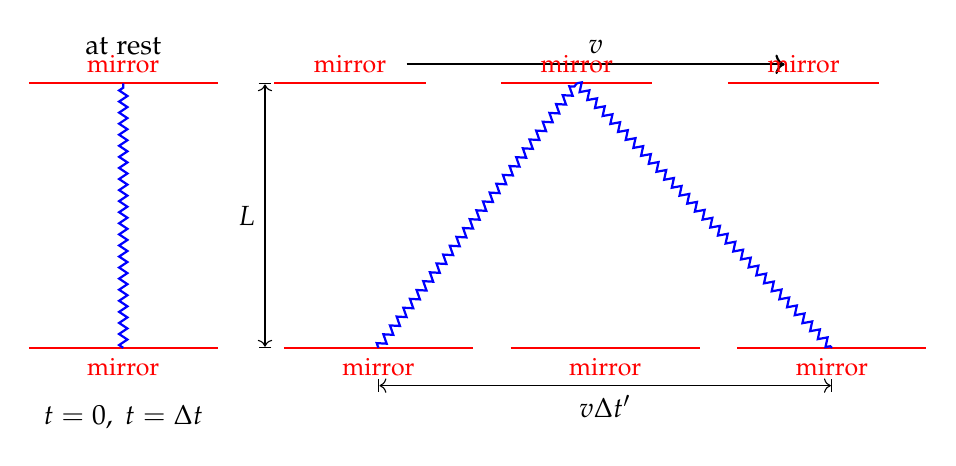
\begin{tikzpicture}[scale=1.2]
    % Stationary Clock
    \node[above] at (0, 3) {at rest};
    \draw[red, thick] (-1, 2.8) -- (1, 2.8) node[midway, above] {\small mirror};
    \draw[red, thick] (-1, 0) -- (1, 0) node[midway, below] {\small mirror};
    \draw[blue, thick, decorate, decoration={zigzag, segment length=4, amplitude=1.5}] (0,0) -- (0,2.8);
    \node[below] at (0, -0.5) {$t=0, \; t=\Delta t$};
    
    % Moving Clock
    \draw[->, thick] (3, 3) -- (7, 3) node[midway, above] {$v$};
    
    \draw[red, thick] (1.6, 2.8) -- (3.2, 2.8) node[midway, above] {\small mirror};
    \draw[red, thick] (4.0, 2.8) -- (5.6, 2.8) node[midway, above] {\small mirror};
    \draw[red, thick] (6.4, 2.8) -- (8.0, 2.8) node[midway, above] {\small mirror};
    
    \draw[red, thick] (1.7, 0) -- (3.7, 0) node[midway, below] {\small mirror};
    \draw[red, thick] (4.1, 0) -- (6.1, 0) node[midway, below] {\small mirror};
    \draw[red, thick] (6.5, 0) -- (8.5, 0) node[midway, below] {\small mirror};
    
    \draw[blue, thick, decorate, decoration={zigzag, segment length=4, amplitude=1.5}] (2.7,0) -- (4.8,2.8);
    \draw[blue, thick, decorate, decoration={zigzag, segment length=4, amplitude=1.5}] (4.8,2.8) -- (7.5,0);
    
    % Distance labels
    \draw[|<->|] (1.5, 0) -- (1.5, 2.8) node[midway, left] {$L$};
    \draw[|<->|] (2.7, -0.4) -- (7.5, -0.4) node[midway, below] {$v\Delta t'$};
\end{tikzpicture}
\end{center}

When we did the light clock calculation of $\Delta t'$ in Lecture 1, we \textit{assumed} that the distance between the mirrors of the light clock remain unchanged when we observe the moving clock. We will now validate the assumption using a \textbf{``proof by contradiction''}.

\textbf{Thought experiment:} Imagine a window in a wall, where the vertical size of the window is \textit{exactly} the same as the height of the light clock -- i.e., the light clock just \textit{barely} fits in the window in an inertial frame in which they are both at rest.

\begin{law}[Exercise 1: Proof by Contradiction]
Now \textit{assume} that the vertical size of an object moving in the horizontal direction is observed to be \textit{smaller} than its size at rest.

With this assumption, make a sketch on your whiteboard of what we would observe for each of the following two scenarios. Do you find a contradiction? Precisely what is being contradicted? How can we resolve the contradiction?

\begin{enumerate}[label=(\alph*)]
    \item The \textit{wall with the window is stationary} and the \textit{light clock is moving} towards the window in the horizontal direction.
    \item The \textit{light clock is stationary} and the \textit{wall with the window is moving} towards the light clock in the horizontal direction.
\end{enumerate}
\end{law}

\section{Transverse and Longitudinal Light Clocks}

Now consider two light clocks, T and L, shown in the figure below.
\begin{itemize}
    \item For Clock T (T for transverse) on the left in the figure, the light propagates perpendicular (transversely) to the horizontal $x$ axis as we initially considered in Lecture 1.
    \item For Clock L (L for longitudinal) on the right in the figure is a light clock of the same construction rotated by $90^\circ$ so that light propagates parallel (longitudinally) to the $x$-axis.
\end{itemize}

\begin{center}
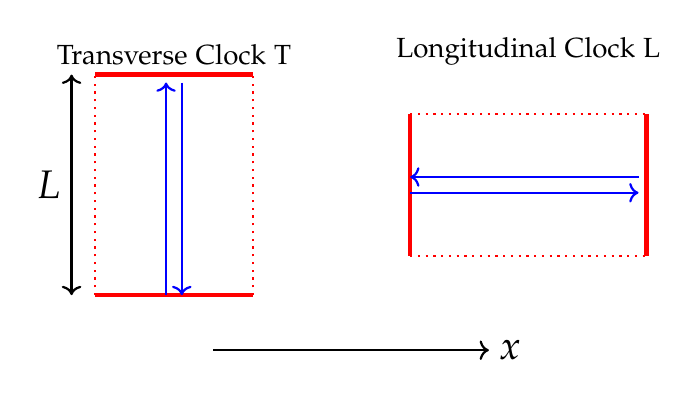
\begin{tikzpicture}[scale=1]
    % Transverse Clock
    \node[above] at (1, 2.8) {Transverse Clock T};
    \draw[red, ultra thick] (0, 2.8) -- (2, 2.8);
    \draw[red, ultra thick] (0, 0) -- (2, 0);
    \draw[red, dotted, thick] (0, 0) -- (0, 2.8);
    \draw[red, dotted, thick] (2, 0) -- (2, 2.8);
    \draw[blue, thick, ->] (0.9, 0) -- (0.9, 2.7);
    \draw[blue, thick, ->] (1.1, 2.7) -- (1.1, 0);
    
    \draw[<->, thick] (-0.3, 0) -- (-0.3, 2.8) node[midway, left] {\Large $L$};

    % Longitudinal Clock
    \node[above] at (5.5, 2.8) {Longitudinal Clock L};
    \draw[red, ultra thick] (4, 0.5) -- (4, 2.3);
    \draw[red, ultra thick] (7, 0.5) -- (7, 2.3);
    \draw[red, dotted, thick] (4, 0.5) -- (7, 0.5);
    \draw[red, dotted, thick] (4, 2.3) -- (7, 2.3);
    \draw[blue, thick, ->] (4, 1.3) -- (6.9, 1.3);
    \draw[blue, thick, ->] (6.9, 1.5) -- (4, 1.5);
    
    % Arrow
    \draw[->, thick] (1.5, -0.7) -- (5, -0.7) node[right] {\Large $x$};
\end{tikzpicture}
\end{center}

Both clocks are at rest in inertial frame $S$, and are calibrated to tick \textit{at the same rate} (while at rest) -- i.e., $\Delta t_{\text{T}} = \Delta t_{\text{L}} \equiv \Delta t$. We say that they are synchronized. As in Lecture 1, we are denoting as $\Delta t$ the time between ticks as measured in frame $S$, the frame in which the clocks are at rest.

\begin{exercise}[Exercise 2]
We are given that Clock T's mirrors are separated by a distance $L$ and that the two Clocks tick at the same rate. Which of the postulates (if any) leads us to conclude that Clock L's mirrors are also separated by a distance $L$?
\end{exercise}

\begin{exercise}[Exercise 3]
Which of the postulates (if any) leads us to conclude that Clock L and Clock T \textit{must} tick at the same rate as each other in another inertial frame $S'$ that is moving with respect to $S$ with constant velocity along the $x$-axis?
\end{exercise}

\begin{exercise}[Exercise 4]
Write down the expression we derived in Lecture 1 for the time between ticks for the transverse Clock T ($\Delta t_{\text{T}}'$) in frame $S'$ in which the clock is moving at constant velocity. First write it in terms of $\gamma$ and $\Delta t$ and then in terms of $\gamma$, $L$, and $c$.
\end{exercise}
\[ \Delta t_{\text{T}}' = \gamma \Delta t = \gamma \frac{2L}{c} \]

\section{Deriving Length Contraction}

Define $\Delta t_{\text{L}}'$ to be the time between ticks for \textit{longitudinal} Clock L in frame $S'$ in which the clock is moving (longitudinally) at constant velocity.

\begin{itemize}
    \item In Exercise 3 above, you concluded that $\Delta t_{\text{L}}' = \Delta t_{\text{T}}'$ by the first postulate.
    \item Therefore, we expect that $\Delta t_{\text{L}}' = \gamma \frac{2L}{c}$, by Exercise 4.
\end{itemize}

In analogy with the light clock calculation from Lecture 1, you will now compute the time between ticks for \textit{longitudinal} Clock L ($\Delta t_{\text{L}}'$) in frame $S'$ in which the clock is moving at constant velocity, \textit{under the assumption that the observed longitudinal distance between the mirrors stays fixed.}

Let's all assume that the inertial observer in frame $S'$ is moving to the left with respect to the clock at speed $v$ so that the light clock is moving to the right at speed $v$ in the $S'$ frame.

\begin{exercise}[Exercise 5]
On your white board, draw a \textit{very} careful diagram of Clock L as seen at three different times in Frame $S'$ (similar to what we did for the transverse light clock); then draw the light paths as the light pulse travels to the right and then (after reflection) to the left.

Use the diagram to find an expression for $\Delta t_{\text{L}}'$, first in terms of $\Delta t$ and then in terms of $\Delta t_{\text{T}}'$. Work this out with your group.

\textit{Hints:}
\begin{itemize}
    \item Try writing expressions for the time the light pulse takes for its rightward journey ($t_+$) and then for its leftward journey ($t_-$). Then $\Delta t_{\text{L}}' = t_+ + t_-$.
    \item Also, remember that the \textbf{distance light travels} in time $t$ ($ct$) equals the \textbf{distance traveled} by the light -- i.e., the distance between where the light started and ended during that part of its journey.
\end{itemize}
\end{exercise}

\[ \Delta t_{\text{L}}' = \text{(Result derived from above exercise)} \]

\begin{exercise}[Exercise 6]
Is your result consistent with Exercises 3 and 4 above? In other words, did you find that $\Delta t_{\text{L}}' = \Delta t_{\text{T}}'$? If not, which \textbf{assumption} (that is valid in Newtonian physics) did you make that may \textbf{not} be valid in relativistic physics?
\end{exercise}

So, we conclude that the observed distance between mirrors for Clock L is \textbf{different} for inertial observers in frame $S$ (in which the clock is stationary) and frame $S'$ (in which the clock is moving).

\begin{exercise}[Exercise 7]
Now use the fact that Clock T and Clock L \textit{must} agree in frame $S'$ (i.e., they must remain synchronized) to identify the observed distance $L'$ between Clock L's mirrors in frame $S'$.
\end{exercise}

\begin{center}
Summary: $L' = \frac{L}{\gamma}$
\end{center}

\begin{exercise}[Exercise 8]
Suppose that a solid ruler of length $L$ is attached between the mirrors of each clock. What would the observed length of each ruler be according to an observer in frame $S'$ (i.e., a frame in which the ruler is moving with respect to the observer)? Why?
\end{exercise}

\section{Conclusion on Length Contraction}
So what have we concluded?
\begin{itemize}
    \item Lengths of moving objects are observed to be shortened (i.e., contracted) along the direction of motion, but not perpendicular to the direction of motion.
\end{itemize}

This is called ``length contraction'' and is our second big result of ``thinking like Einstein''!

But is it true that lengths of moving objects are observed to be contracted in the direction of the motion? Does this really happen?? Yes! Read Example 2 (Muon Decay, again) on p. 26 in the textbook by Morin for an example of experimental evidence for length contraction.

Compare and contrast this example to Example 2 (Muon Decay) on p. 23 where the same situation was interpreted as time dilation!

We will now use time dilation again to derive ``length contraction'' -- but in a different way.

% --- Continuation of Lecture 2 ---

\section{Length Contraction Again}

Let's use a clock to measure distance in another way---by measuring the amount of time it takes for a moving object to pass by an inertial observer with known speed $v$.

\begin{itemize}
    \item Consider a long ruler of length $L_0$, as measured in an inertial frame in which the \textit{ruler is at rest}.
    \item Suppose the ruler is now moving past us at constant velocity $\vec{v}$ (speed $v$).
    \item With a clock at rest in our frame, we measure the time $\Delta t$ that it takes the ruler to pass.
\end{itemize}

See figure below.
\begin{itemize}
    \item We are the inertial observer holding the stopwatch (our ``clock'') that reads $\Delta t$. We do not know the length of the ruler but we know it is moving past us at speed $v$.
    \item Another inertial observer is moving \textit{with} the ruler (imagine the observer is standing on the ruler) and measures its length to be $L_0$.
    \item The position of the ruler is shown at time $t_1$ and again at time $t_2 = t_1 + \Delta t$.
\end{itemize}

\begin{center}
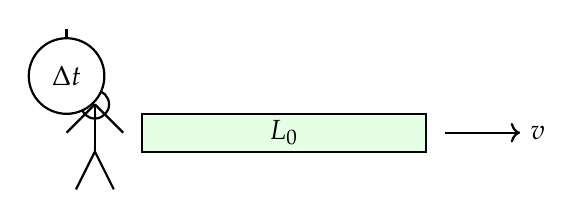
\begin{tikzpicture}[scale=1.2]
    % Ruler passing by the observer
    \draw[thick, fill=green!10] (0, 0) rectangle (3, 0.4);
    \node at (1.5, 0.2) {$L_0$};
    \draw[->, thick] (3.2, 0.2) -- (4, 0.2) node[right] {$v$};
    
    % Stick figure observer
    \draw[thick] (-0.5, 0) -- (-0.5, 0.5);
    \draw[thick] (-0.5, 0.5) circle (0.15);
    \draw[thick] (-0.5, 0.5) -- (-0.8, 0.2);
    \draw[thick] (-0.5, 0.5) -- (-0.2, 0.2);
    \draw[thick] (-0.5, 0) -- (-0.7, -0.4);
    \draw[thick] (-0.5, 0) -- (-0.3, -0.4);
    
    % Stopwatch
    \draw[thick, fill=white] (-0.8, 0.8) circle (0.4) node {$\Delta t$};
    \draw[thick] (-0.8, 1.2) -- (-0.8, 1.3);
\end{tikzpicture}
\end{center}

\begin{exercise}[Exercise 9]
What is the length $L_{\text{m}}$ of the \textit{moving} ruler that we \textit{calculate}?
\end{exercise}
\[ L_{\text{m}} = \]

Now take the perspective of the observer moving \textit{with} the ruler. That observer measures the time $\Delta t'$ that it takes our clock (which is \textit{moving} at speed $v$ in the observer's rest frame) to pass by the ruler (which is \textit{stationary} in the observer's frame).

\begin{exercise}[Exercise 10]
Make a sketch to the right of the above sketch showing the situation from the perspective of the observer moving with the ruler, at times $t_1$ and $t_2$. What is the length $L_0$ of the ruler that this observer calculates?\\
(Assume that this observer has attended Lecture 1 of PHYSICS 61 and understands how to apply the concept of time dilation!)
\end{exercise}
\[ L_0 = \]

\begin{exercise}[Exercise 11]
Now use these results to (re)derive the length contraction formula ($L_{\text{m}}$ in terms of $L_0$):
\end{exercise}
\[ \frac{L_{\text{m}}}{L_0} = \]
\[ \implies L_{\text{m}} = \]

Since $\gamma \ge 1, L_{\text{m}} \le L_0 \implies$ length contraction (again)!

\section{Events in Spacetime}

An \textbf{event} is a point in ``spacetime'' -- i.e., it is the position \textit{and} time at which something happens. For example, in the situation described above,
\begin{itemize}
    \item Event 1 corresponds to the time and position at which the \textbf{right} end of the ruler is exactly lined up with the observer with the stationary clock.
    \item Event 2 corresponds to the time and position at which the \textbf{left} end of the ruler is exactly lined up with the observer with the stationary clock.
\end{itemize}

In Newtonian physics, observers in different frames may not agree on the position and time coordinates at which an event happens, but (as you argued in Lecture 1) they \textbf{will agree} on the difference in time between when two events occur \textit{and} on the length of objects -- i.e., the distance between the location of the ends of the object, measured at the same time.

In special relativity, due in part to time dilation and length contraction, different observers will \textbf{not} generally agree on either the time between two events, or the distance between two events that happen at the same time (e.g., the difference between the position of the two ends of an object measured simultaneously).

We will generalize these results to arbitrary events in ``spacetime'' over the course of the next few lessons.

% ==================== LECTURE 3 ====================
\chapter{Seeing vs.\ Observing; Relativity of Simultaneity}

\section{Seeing is Not Observing!}

It's important to distinguish between \textit{seeing} and \textit{observing} in special relativity. Although there is no standard terminology in textbooks, etc., we'll try to consistently use the following definitions.

\begin{itemize}
    \item \textbf{Seeing} means `light emitted from an event is focused and perceived by my eye' (or by a camera or other detection device). This always happens \textit{after} the event, due to the finite speed of light. We will also describe measurements based on \textit{seeing} as how the situation \textit{appears} -- for example, we might refer to ``apparent size.''
    \item \textbf{Observing} means `light emitted from an event is detected by my eye, and I \textit{correct} for the time delay due to the finite speed of light to calculate the \textit{actual} time and position at which the event happened.'
\end{itemize}

We will almost always mean `observing' even when we don't say it. (Indeed, we've meant `observing' for everything so far.) But to illustrate the difference, we will now calculate the \textit{apparent} length of a ruler when it is moving lengthwise toward us.

\section{Apparent Length of a Moving Ruler}

Assume that a ruler (rest length $L$) is moving end-on towards an observer at speed $v$.

\begin{exercise}[Exercise 1]
What is the observed length of the moving ruler?
\end{exercise}
\begin{solution}
$L' = \frac{L}{\gamma}$
\end{solution}

Assume that the front end of the ruler reaches the observer at time $t=0$. At the same time ($t=0$), light from the back end of the ruler is also reaching the observer. But the ruler was further away when the light from the back end was actually emitted at some time interval $\Delta t$ earlier.

Make a sketch showing the position of the ruler at $t=0$ and at $t=-\Delta t$.

\begin{center}
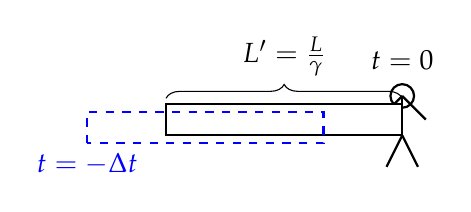
\begin{tikzpicture}[scale=1]
    % Observer
    \draw[thick] (0,0) -- (0,0.5);
    \draw[thick] (0,0.5) circle (0.15);
    \draw[thick] (0,0.5) -- (-0.3,0.2);
    \draw[thick] (0,0.5) -- (0.3,0.2);
    \draw[thick] (0,0) -- (-0.2,-0.4);
    \draw[thick] (0,0) -- (0.2,-0.4);
    \node[above] at (0, 0.7) {$t=0$};

    % Ruler at t=0
    \draw[thick, fill=white] (-3, 0) rectangle (0, 0.4);
    \draw [decorate,decoration={brace,amplitude=5pt},xshift=0pt,yshift=2pt]
      (-3,0.4) -- (0,0.4) node [black,midway,yshift=15pt] {$L' = \frac{L}{\gamma}$};

    % Ruler at t=-Delta t (dashed)
    \draw[dashed, blue, thick] (-4, -0.1) rectangle (-1, 0.3);
    \node[blue, below] at (-4, -0.1) {$t = -\Delta t$};
\end{tikzpicture}
\end{center}

\begin{exercise}[Exercise 2]
Find an expression for $\Delta t$ -- i.e., the time interval between when the light left the back of the ruler and when it reaches our eye.\\
(Set the distance light travels in time $\Delta t$ equal to the distance traveled.)
\end{exercise}
\begin{solution}
$c\Delta t = \text{distance traveled} = v\Delta t + L'$
\end{solution}

Solving for $\Delta t$:
\[ c\Delta t = L' + v\Delta t \]
\[ \Delta t = \frac{L'}{c-v} = \frac{L/\gamma}{c-v} = \frac{L \sqrt{1-v^2/c^2}}{c-v} = \frac{L}{c \gamma (1-v/c)} \]

\begin{exercise}[Exercise 3]
So how long does the ruler \textit{appear} to be? Let's call this the \textit{apparent} length $L_{\text{app}}$. Use $\gamma = \frac{1}{\sqrt{1-v^2/c^2}}$ to express $L_{\text{app}}$ in terms of $L$ and $v/c$.
\end{exercise}
\begin{solution}
\[ L_{\text{app}} = c\Delta t = \frac{L}{\gamma (1-v/c)} = L \frac{\sqrt{1-v^2/c^2}}{1-v/c} = L \frac{\sqrt{1+v/c}}{\sqrt{1-v/c}} > L \]
\end{solution}

This artifact, due to the finite speed of light, is sometimes called \textit{aberration}.

\begin{exercise}[Exercise 4]
Now rank the `proper length' $L$, the observed length $L'$, and the apparent length $L_{\text{app}}$ from shortest to longest, for $v > 0$.
\end{exercise}
\begin{solution}
Ranked order for ruler moving toward observer: \quad $L' < L < L_{\text{app}}$
\end{solution}

\begin{exercise}[Quick Exercise 5]
What if the ruler is instead moving away from us? Will it \textit{appear} to be longer or shorter than $L$? How about compared to $L'$?
\end{exercise}
\begin{solution}
Ranked order for ruler moving away from observer: \quad $L_{\text{app}} < L' < L$
\end{solution}

\section{Relativity of Simultaneity}

In Newtonian mechanics, events that are observed to be simultaneous in one reference frame (i.e., they are observed to occur at the same time) are also simultaneous in all other frames. You will now show that this is no longer true in special relativity.

Consider the following scenario involving two inertial observers: Ada on Earth and Bob in a spacecraft. We will use ``unprimed'' symbols ($x$ and $t$) for Ada's frame, and primed symbols ($x'$ and $t'$) for Bob's frame.
\begin{itemize}
    \item Two flash bulbs (labeled \#1 and \#2) are stationary at $x = \pm L$ and fire simultaneously in Ada's inertial frame.
    \item Ada, standing at $x = 0$, \textit{sees} the flashes (simultaneously) at time $t=0$.
    \item At that instant, Bob flies by (to the right) at speed $v$, and also \textit{sees} the flashes simultaneously, at $t'=0$.
\end{itemize}

So, Ada, Bob, and both flashes of light must -- for just an instant -- be at the same place at the same time: $x'=x=0$ at $t'=t=0$. (This must be true in all frames since otherwise the 1st postulate would be violated -- think about it.)

\begin{exercise}[Exercise 6]
Make sketches of the situation \textbf{in Ada's inertial frame} at two different times:
\begin{enumerate}[label=\alph*.]
    \item when the bulbs flash (i.e., the flashes are about to leave each bulb);
    \item when Ada and Bob see the flashes (i.e., the flashes are detected by Ada and Bob).
\end{enumerate}
\end{exercise}
\begin{solution}
\textit{(Sketches included in original notes showing bulbs firing at $x=\pm L$ at $t < 0$, and reaching $x=0$ at $t=t'=0$.)}
\end{solution}

In the following, assume that Ada and Bob have understood the first two lectures of PHYSICS 61 and are capable of making \textit{observations} based on what they \textit{see}.

\begin{exercise}[Exercise 7]
We are given that Ada sees the flashes at $t=0$. At what times $t_1$ and $t_2$ does Ada observe bulbs 1 and 2 to flash? (Think about whether $t_1$ and $t_2$ are positive or negative...)
\end{exercise}
\begin{solution}
\[ t_1 = t_2 = -\frac{L}{c} \]
Since $t_1 = t_2$, the events are simultaneous in Ada's frame.
\end{solution}

Bob \textit{observes} a more complicated situation. He \textit{sees} both flashes at $t'=0$, but in his reference frame the flash bulbs are moving, \textit{and} he observes the distance between them to be length-contracted.

You will now determine the travel times of the light from bulb \#1 and \#2 in Bob's inertial frame: $\Delta t_1'$ and $\Delta t_2'$. Then $-\Delta t_1'$ and $-\Delta t_2'$ are the times at which Bob \textit{observes} the flashes to occur. Our goal is to answer these two questions:
\begin{enumerate}[label=\roman*.]
    \item Does Bob observe the bulbs to flash at the same time as Ada observes them to flash?
    \item If not, does Bob at least observe the bulbs to flash \textit{simultaneously} -- as Ada does??
\end{enumerate}

\begin{exercise}[Exercise 8]
Begin by carefully sketching the situation in Bob's frame (what Bob observes) at the instant when Ada and Bob simultaneously \textit{see} the flashes of light. Label any distances with appropriate symbols and/or expressions.
\end{exercise}

\begin{solution}
\textit{(Sketch showing Bob moving to the right, identifying distance $L'$ for the contracted length of each side to the flashes, and arrows showing the light coming toward Bob at $x'=0$.)}
\end{solution}

\begin{exercise}[Exercise 9]
In which direction are Ada and the bulbs moving with velocity $v$ in Bob's frame?
\end{exercise}
\begin{solution}
To the left.
\end{solution}

\begin{exercise}[Exercise 10]
Now make a sketch illustrating the location at which each bulb flashed in Bob's frame, labeling any distances with appropriate symbols.
\end{exercise}
\begin{solution}
\textit{(Sketch showing Left bulb flashing at $x' = -L'$, Right bulb flashing at $x' = L'$.)}
\end{solution}

\begin{exercise}[Exercise 11]
Now equate ``\textit{the distance light travels in time $\Delta t$''} to ``\textit{the distance traveled in that time}'' to find expressions for $\Delta t_1'$ and $\Delta t_2'$ in terms of $L$ and $v/c$. You should see parallels with earlier calculations!
\end{exercise}
\begin{solution}
For bulb 1 (left bulb, moving left):
\[ c\Delta t_1' = L' - v\Delta t_1' \implies \Delta t_1' = \frac{L'}{c+v} = \frac{L\sqrt{1-v^2/c^2}}{c(1+v/c)} = \frac{L}{c}\frac{\sqrt{1-v/c}}{\sqrt{1+v/c}} \]

For bulb 2 (right bulb, moving left):
\[ c\Delta t_2' = L' + v\Delta t_2' \implies \Delta t_2' = \frac{L'}{c-v} = \dots = \frac{L}{c}\frac{\sqrt{1+v/c}}{\sqrt{1-v/c}} \]
\end{solution}

\begin{exercise}[Exercise 12]
So, does Bob \textit{observe} the bulbs to flash at the same time? If not, which bulb does Bob observe to flash first (i.e., earlier than the other)?
\end{exercise}
\begin{solution}
No. The right one flashes first since it's further away.
\end{solution}

\begin{exercise}[Exercise 13]
What does this say about simultaneity? (Make a precise statement.)
\end{exercise}
\begin{solution}
It doesn't exist (in an absolute sense across reference frames).
\end{solution}

This important result is called ``\textbf{Relativity of Simultaneity}''.

\section{Optional: Comparing to the Textbook}

\begin{exercise}[Exercise 14]
Calculate the difference between the times at which the two bulbs flash as observed by Bob.
\end{exercise}
\[ \Delta t_2' - \Delta t_1' = \]
\[ = \]
\[ = \frac{2L\gamma v}{c^2} \qquad \text{Used } \gamma^2 = 1/(1-v^2/c^2). \]

\begin{exercise}[Exercise 15]
The figure below shows a snippet from Sec. 1.3.1 in the textbook by Morin. The clocks at the front and back of the moving train are synchronized in the frame of the train. Read this result from the textbook:

\begin{center}
\fbox{
\begin{minipage}{0.8\textwidth}
\textbf{REAR-CLOCK-AHEAD:} If a train with length $L$ moves with speed $v$ relative to you, then you observe the rear clock reading $Lv/c^2$ more than the front clock, at any given instant.
\end{minipage}
}
\end{center}

The synchronized clocks in Morin's example are analogous to the synchronized flash bulbs in Ada's frame, and the observer on the ground in Morin's example is analogous to Bob.

Explain how to reconcile differences between the result you just derived and the ``rear clock ahead'' result derived in the textbook. Are the results completely consistent?

Hint: The results are indeed consistent... The factor of 2 is straightforward. How about the factor of $\gamma$?
\end{exercise}

% ==================== LECTURE 4 ====================
\chapter{Spacetime Diagrams}

\section{An Aside on some Terminology}

\begin{itemize}
    \item An \textbf{event} is a point in spacetime -- in other words, the position \textit{and} time of something that happens. (Observers in different inertial frames may disagree about the position and time of the same event.)
    \item The \textbf{coordinate time} is the time measured by an inertial observer -- i.e., an observer at rest in a particular inertial reference frame. Given this definition, observers in different inertial frames can disagree about the \textit{coordinate time interval} between two events. Examples:
    \begin{itemize}
        \item Time dilation!
        \item The different interval of time between when bulbs 1 and 2 flash as observed by Ada and Bob in their different inertial frames, in Lecture 3 (Relativity of Simultaneity).
    \end{itemize}
    \item The \textbf{proper time} between events is the \textit{time interval} measured by an inertial clock that is actually present at both events. More generally, the proper time is the time between two events, as measured in the inertial frame in which the events happen at the same place.
    \begin{itemize}
        \item All observers will \textbf{calculate} the same \textit{proper} time between events -- by correcting for known time dilation, for example.
        \item Proper time intervals are often denoted $\Delta \tau$ ($\tau$ = Greek letter \textit{tau}) to distinguish them from coordinate time intervals $\Delta t$.
    \end{itemize}
\end{itemize}

\begin{exercise}[Quick Questions]
In the first light-clock thought experiment you derived the time dilation result, $\Delta t' = \gamma \Delta t$. Circle the correct response (True or False) and then check your responses and justifications with your neighbor.

\begin{itemize}
    \item $\Delta t$ is a coordinate time interval. \qquad \textbf{True} / False
    \item $\Delta t$ is a proper time interval. \qquad \textbf{True} / False
    \item $\Delta t'$ is a coordinate time interval. \qquad \textbf{True} / False
    \item $\Delta t'$ is a proper time interval. \qquad True / \textbf{False}
\end{itemize}
\end{exercise}

We will now discuss how to draw diagrams of spacetime from the point of view of multiple inertial observers. Far from being simple pictures, spacetime diagrams are powerful tools for visualizing relativity problems, and will help us transition to more complicated situations.

\section{Quick Review: `Space--Space Diagrams'}

Before we dive into creating diagrams of spacetime (two-dimensional graphs of position and time), we will first review some of the key facts about another sort of two-dimensional graph: the Cartesian $x$--$y$ plane. (Pay close attention to details so that you will be able to identify how spacetime diagrams are the \textbf{same} or \textbf{different}!)

\begin{exercise}[Exercise 1]
Draw a simple $x$-$y$ graph. As we go through each of the features described in points (a) - (f) below, fill in any blanks and/or sketch on the graph an example that illustrates the feature.
\end{exercise}

\begin{center}
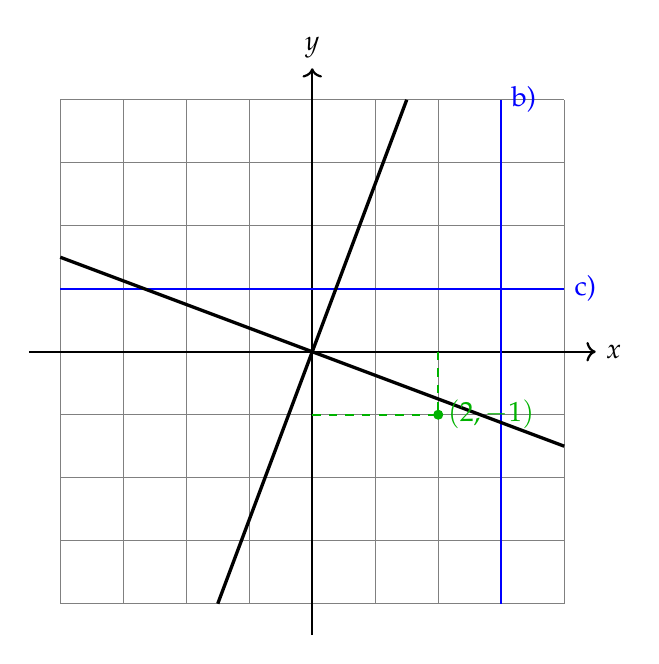
\begin{tikzpicture}[scale=0.8]
    % Grid
    \draw[step=1cm,gray,very thin] (-4,-4) grid (4,4);
    % Axes
    \draw[thick,->] (-4.5,0) -- (4.5,0) node[right] {$x$};
    \draw[thick,->] (0,-4.5) -- (0,4.5) node[above] {$y$};
    
    % Feature sketches based on student notes
    \draw[blue, thick] (3, -4) -- (3, 4) node[right] {b)};
    \draw[blue, thick] (-4, 1) -- (4, 1) node[right] {c)};
    
    \draw[very thick] (-4, 1.5) -- (4, -1.5);
    \draw[very thick] (-1.5, -4) -- (1.5, 4);
    
    % Point coordinate trace
    \draw[green!70!black, dashed, thick] (2,0) -- (2,-1);
    \draw[green!70!black, dashed, thick] (0,-1) -- (2,-1);
    \filldraw[green!70!black] (2,-1) circle (2pt) node[right] {$(2, -1)$};
\end{tikzpicture}
\end{center}

\begin{enumerate}[label=(\alph*)]
    \item $x$ and $y$ axes are perpendicular and cross at $x=y=0$.
    \item ``Lines of constant $x$'' are parallel to the \textbf{[$y$]} axis.
    \item ``Lines of constant $y$'' are parallel to the \textbf{[$x$]} axis.
    \item The axes themselves are such lines: the $y$-axis is the line along which \textbf{[$x$]} = 0, and the $x$-axis is the line along which \textbf{[$y$]} = 0.
    \item The coordinates of a point can be read off the axes by drawing a pair of lines from the point to the coordinate axes, where the lines are each perpendicular to one axis and parallel to the other axis (these are equivalent since the axes cross at a right angle).
    \item We can construct a second coordinate system with the same origin but \textit{rotated} with respect to the first (the `primed' coordinates), and read off new coordinates for the same points.
    
    Although the \textit{coordinates} of points in the plane are different in the rotated system, \textit{geometry} (including distances between pairs of points and angles between pairs of lines) is the same.
\end{enumerate}

\section{Spacetime Diagrams}

Spacetime diagrams are graphs in the $x$--$t$ plane instead of the $x$--$y$ plane.
\begin{itemize}
    \item For now, we will limit ourselves to one spatial dimension, $x$; i.e., we are considering objects for which the only spatial coordinate of interest is $x$.
    \item Traditionally, the $x$ axis points to the right in a spacetime diagram, and the $t$ axis points \textit{up} (rather than to the right as you are probably used to from classical mechanics).
\end{itemize}

\begin{center}
\begin{tikzpicture}[scale=1]
    \draw[thick] (-2,0) -- (2,0) node[right] {$x$};
    \draw[thick] (0,-2) -- (0,2) node[above] {$ct$};
\end{tikzpicture}
\end{center}

There are a few key differences between spacetime diagrams and space--space diagrams:

\begin{itemize}
    \item \textbf{\textcolor{blue}{Question:}} \textcolor{blue}{`Points' on a spacetime diagram do \textit{not} represent geometric points (in space). Instead they represent... what?} \textit{(Answer: Events)}
    \item The dimensions (and therefore the SI units) of space and time are different.
    \begin{itemize}
        \item To make the dimensions the same, we typically multiply time $t$ by the speed of light $c$ (think of $c$ here as a constant of nature that conveniently has dimensions of length over time) and then plot $x$ on the horizontal axis and $ct$ on the vertical axis so both have dimensions of length.
        \item We can then use the same units for both the $x$ and $ct$ axes -- say, meters.
        \item However, in special relativity, there are more \textit{relevant and useful units} -- for example:
        \begin{itemize}
            \item the light-second (the distance light travels in one second: 1 $\ell\text{s} = c \times 1\text{ s}$),
            \item the light-year (the distance light travels in one year: 1 $\ell\text{year} = c \times 1\text{ year}$).
        \end{itemize}
        \item And we can choose to use the same scale on each axis (e.g., 1 light-second between equally spaced tick marks on each axis).
    \end{itemize}
\end{itemize}

[\textbf{Optional} aside: It is possible to choose so-called `natural' units in which $c$ has a numerical value of 1. For example, if we use light-seconds ($\ell$s) for distance and seconds (s) for time, then $c = 1 \, \ell\text{s/s}$. You will learn about this and other fundamental ``natural units'' later in the quarter. Sometimes physicists (and textbooks) drop any factor of $c$ when using natural units (more precisely, they are setting the value equal to 1), but we will always explicitly write the factors of $c$ in this class to make dimensional consistency apparent.]

\section{Worldlines}

Draw a set of spacetime axes and use them for the following exercises.

\begin{exercise}[Exercise 2]
If points on a spacetime diagram represent events, what does an object at rest look like in a spacetime diagram? Draw a couple of examples of objects at rest at different positions on your spacetime diagram.
\end{exercise}

\begin{center}
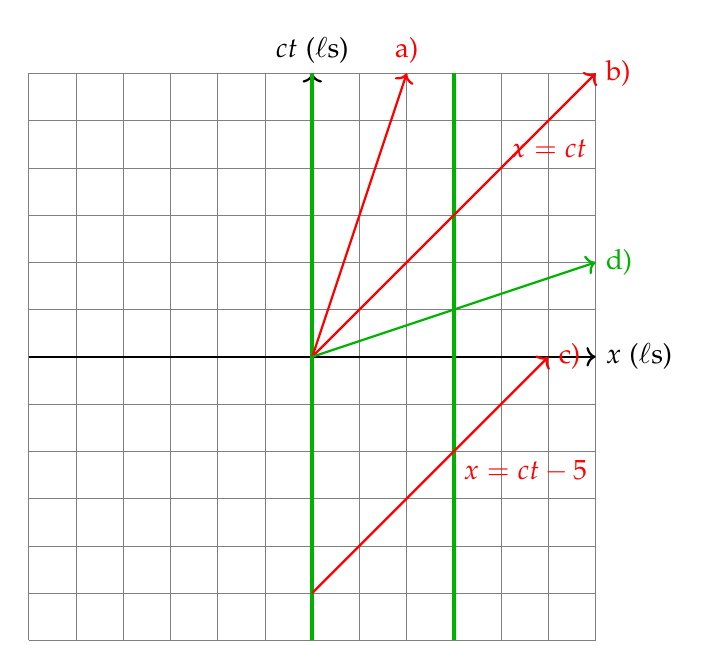
\begin{tikzpicture}[scale=0.6]
    % Grid
    \draw[step=1cm,gray,very thin] (-6,-6) grid (6,6);
    % Axes
    \draw[thick,->] (-6,0) -- (6,0) node[right] {$x$ ($\ell$s)};
    \draw[thick,->] (0,-6) -- (0,6) node[above] {$ct$ ($\ell$s)};
    
    % Object at rest (green line on ct axis and another)
    \draw[green!70!black, ultra thick] (0,-6) -- (0,6);
    \draw[green!70!black, ultra thick] (3,-6) -- (3,6);
    
    % Exercise 3 lines (recreated from student annotations)
    \draw[red, thick, ->] (0,0) -- (2,6) node[above] {a)};
    \draw[red, thick, ->] (0,0) -- (6,6) node[right] {b)};
    \node[red, above right] at (4,4) {$x=ct$};
    \draw[red, thick, ->] (0,-5) -- (5,0) node[right] {c)};
    \node[red, below right] at (3,-2) {$x=ct-5$};
    \draw[green!70!black, thick, ->] (0,0) -- (6,2) node[right] {d)};
\end{tikzpicture}
\end{center}

\textbf{Definition of a ``worldline''}: In general, an object undergoing arbitrary motion will make a line (or a curve) on the spacetime diagram, called the \textit{worldline} of the object. Mathematically, the worldline of object $\mathcal{O}$ is the following collection of events:
\[ \{ (x, ct) | \text{object } \mathcal{O} \text{ is at point } x \text{ at time } t \}. \]

\begin{exercise}[Exercise 3]
What do the worldlines look like for the following examples? Sketch them on your whiteboard and label them (a) through (d). For (b) and (c), try writing an equation that describes the worldline.
\begin{enumerate}[label=(\alph*)]
    \item An object moving to the right with a small constant velocity. (``Small'' compared to what?) \textcolor{red}{Light.}
    \item A flash of light moving to the right, emitted from the origin ($x=0$) at $t=0$.
    \item A flash of light moving to the right, emitted from the origin ($x=0$) at $ct = -5$ light seconds. \textit{(Note: the original text says "to the left", but the drawn line goes to the right!)}
    \item Object moving faster than the speed of light -- assuming that were possible!
\end{enumerate}
\end{exercise}

A very important fact about worldlines is that the worldline of \textit{light} always has a slope of $\pm 1$ in the spacetime diagram (Einstein's 2nd postulate!) and the angle between the worldline and either the $x$ or $ct$ axis will be 45-degrees (if the axes have the same scale).

\begin{exercise}[Quick Question]
How would we represent an \textit{extended} object (e.g., a ruler lying at rest along the $x$ axis or moving along the $x$ axis with constant velocity) on a spacetime diagram?
\end{exercise}

\begin{exercise}[Exercise 4]
\begin{enumerate}[label=(\alph*)]
    \item Carefully sketch the worldline of a clock moving to the right at constant speed $3c/5$. (Assume it passes $x=0$ at $t=0$.) What is the slope of the line?
    \item The clock ticks every second \textit{in its rest frame} -- i.e., $\Delta \tau = 1$ s. Mark several ``clock tick'' events on your diagram \textit{at the correct locations}. (Yes, you will need to do a calculation to correctly locate the tick marks!)
\end{enumerate}
\end{exercise}

\begin{solution}
For (a): The velocity is $v = \frac{3c}{5}$, which means $x = \frac{3c}{5}t \implies \frac{ct}{x} = \frac{5}{3}$. The slope on the $x$--$ct$ diagram is $\frac{5}{3}$.\\
For (b): Time dilation says $\Delta t = \gamma \Delta \tau$.
\[ \gamma = \frac{1}{\sqrt{1-(3/5)^2}} = \frac{1}{\sqrt{16/25}} = \frac{5}{4} = 1.25 \]
So $\Delta t = 1.25$ s. The coordinates for the ticks are $(x, ct) = (v\Delta t, c\Delta t) = (3/4, 5/4), (6/4, 10/4), (9/4, 15/4), (3, 5)$, etc.
Notice that for the first tick, $\sqrt{(ct)^2 - x^2} = \sqrt{(5/4)^2 - (3/4)^2} = \sqrt{16/16} = 1 = c\Delta \tau$.
\end{solution}

\begin{center}
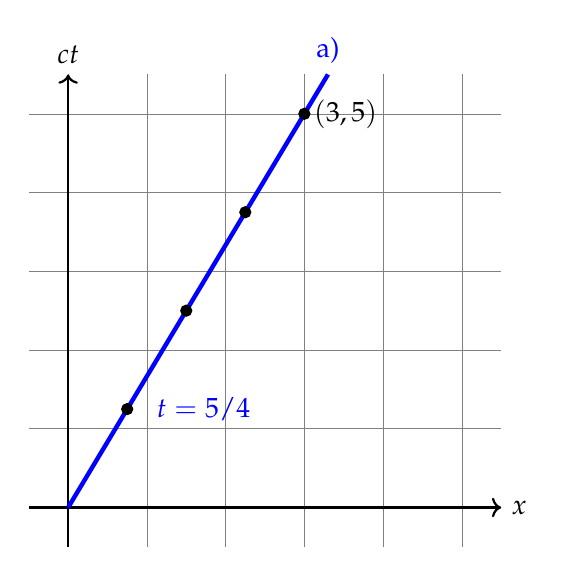
\begin{tikzpicture}[scale=1]
    % Grid
    \draw[step=1cm,gray,very thin] (-0.5,-0.5) grid (5.5,5.5);
    % Axes
    \draw[thick,->] (-0.5,0) -- (5.5,0) node[right] {$x$};
    \draw[thick,->] (0,-0.5) -- (0,5.5) node[above] {$ct$};
    
    % Worldline
    \draw[ultra thick, blue] (0,0) -- (3.3, 5.5) node[above] {a)};
    
    % Ticks
    \filldraw[black] (0.75, 1.25) circle (2pt);
    \filldraw[black] (1.5, 2.5) circle (2pt);
    \filldraw[black] (2.25, 3.75) circle (2pt);
    \filldraw[black] (3, 5) circle (2pt) node[right] {$(3, 5)$};
    
    \node[right, blue] at (1, 1.25) {$t=5/4$};
\end{tikzpicture}
\end{center}

\textbf{Summary} -- In analogy with the points we made about the $x$--$y$ coordinate axes (above), we can make the following general statements:
\begin{itemize}
    \item \textbf{Vertical lines} in the $(x, ct)$ spacetime diagram connect all events that happen at the same \textbf{[place]}.
    
    In particular, the \textbf{[$ct$]} axis is the line on the diagram that connects all events that happen at $x=0$.
    
    It is also the worldline of an object at rest according to an inertial observer in the $(x, ct)$ frame.
    \item \textbf{Horizontal lines} in the $(x, ct)$ spacetime diagram connect all events that happen at the same \textbf{[time]}.
    
    In particular, the \textbf{[$x$]} axis itself connects the set of all events that happen at $t=0$.
    
    In other words, the $x$ axis connects all events that are \textit{simultaneous} with an event at the origin of spacetime ($x=t=0$), according to an inertial observer in the $(x, ct)$ frame.
\end{itemize}

\section{A Second Frame of Reference: The ``Primed'' Axes}

Now it's time to see what a second coordinate system (or inertial frame of reference) looks like superimposed on the first. (This is \textit{somewhat} analogous to drawing a rotated $x'$--$y'$ coordinate system on an $x$--$y$ plane, except that importantly we are dealing with space and time -- in special relativity!)

First, we need to carefully define what the new $t'$ and $x'$ coordinate axes \textit{represent} in order to draw them.

In analogy with the points we just made about the unprimed $(x, ct)$ coordinate axes, we can write the following:
\begin{itemize}
    \item The $t'$ axis is the line on the diagram that connects all events that happen at $x'=0$.
    
    It is also the worldline of an object at rest according to an inertial observer in the $(x', ct')$ frame.
    \item The $x'$ axis is the set of all events that happen at $t'=0$.
    
    In other words, it is all events that are \textit{simultaneous} with an event at the origin of spacetime ($x'=t'=0$), according to an observer in the $(x', ct')$ frame.
\end{itemize}

\begin{exercise}[Quick Question]
From above, we have already drawn one of the axes for a viable primed frame (including the tick marks!), in the form of the worldline for the inertial clock. Which axis did we draw ($x'$ or $ct'$)? How would you describe the corresponding inertial frame?
\end{exercise}

\begin{itemize}
    \item Now we need to draw the other axis, the \textbf{[$x'$]} axis -- i.e., the line that connects events that are \textit{simultaneous} in the primed frame.
    \item As you'll now see, we can use our existing \textbf{[$ct'$]} axis, and the fact that light travels on 45-degree worldlines in spacetime, to help us.
\end{itemize}

And as we've done in the past, we'll use a thought experiment involving flashes of light!

\begin{exercise}[Exercise 5]
On your whiteboard, make a sketch of the following sequence of three events in real space (i.e., one-dimensional physical space, along the $x'$ axis). Label each event with its time $t'$ and position $x'$.
\begin{enumerate}[label=(\alph*)]
    \item Event A: At time $t' = -T$, a light flash is sent in the positive $x$ direction from the location of a clock that is \textit{at the spatial origin} of the primed frame.
    \item Event B: At time $t' = 0$, the light flash is reflected back in the negative $x$ direction.
    \item Event C: At time $t' = +T$, the light flash is detected at the location of the original clock.
\end{enumerate}
\end{exercise}

\begin{solution}
\textit{(Sketch showing Event A at $-T$ on a vertical $ct'$ axis, sending light rightward. At $t'=0$, it reflects at Event B, and travels leftward back to Event C at $+T$ on the $ct'$ axis.)}
\end{solution}

\begin{exercise}[Exercise 6]
On your whiteboard, carefully draw the set of events (A, B, C) on a spacetime diagram like the one below, for some arbitrary value of $T$. (We have already included the $ct'$ axis you sketched above.) \textbf{Hints:}
\begin{enumerate}[label=(\alph*)]
    \item First try locating events A and C on the spacetime diagram.
    \item Then draw the worldline for a flash of light traveling to the right \textit{from} A.
    \item Now draw the worldline for a flash of light traveling to the left \textit{toward} C. (It may be helpful to remember that light travels at speed $c$ in all inertial frames, and to recall the worldlines you drew earlier for rightward and leftward traveling light flashes!)
\end{enumerate}
What does the point of intersection of these two worldlines represent??
\end{exercise}

\begin{center}
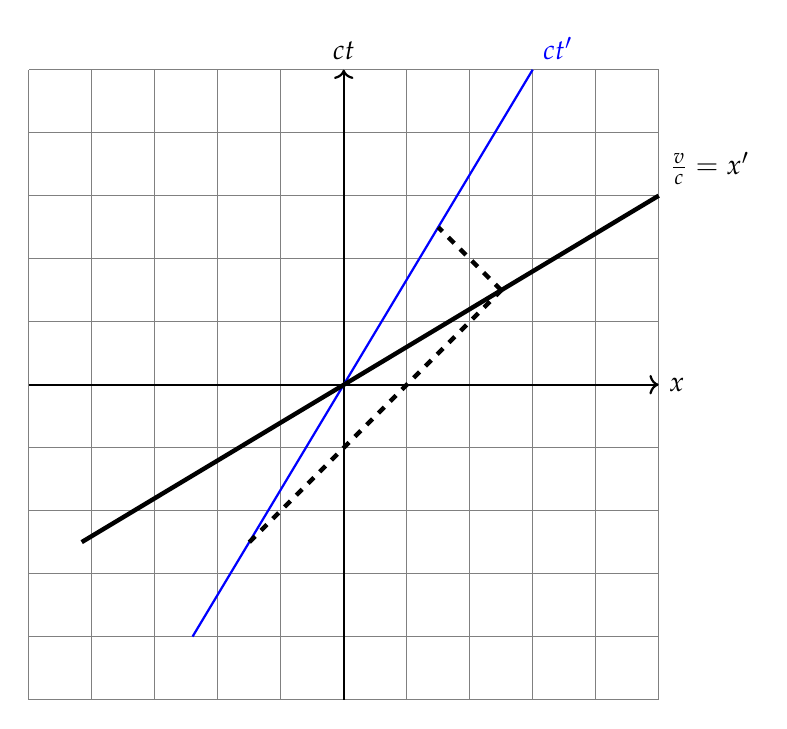
\begin{tikzpicture}[scale=0.8]
    % Grid
    \draw[step=1cm,gray,very thin] (-5,-5) grid (5,5);
    % Axes
    \draw[thick,->] (-5,0) -- (5,0) node[right] {$x$};
    \draw[thick,->] (0,-5) -- (0,5) node[above] {$ct$};
    
    % ct' axis (slope 5/3)
    \draw[blue, thick] (-2.4, -4) -- (3, 5) node[above right] {$ct'$};
    
    % Events A, B, C
    % Let T = 2.5 on the ct' axis.
    % ct' axis unit vector is (3/5, 1) rescaled so ct^2 - x^2 = 1.
    % Actually just use points on the line. Let's pick A=(-1.5, -2.5) and C=(1.5, 2.5).
    % Event A:
    \coordinate (A) at (-1.5, -2.5);
    % Event C:
    \coordinate (C) at (1.5, 2.5);
    
    % Light from A (slope 1)
    % Light to C (slope -1)
    % Intersection B: 
    % L1: ct - (-2.5) = x - (-1.5) => ct = x - 1
    % L2: ct - 2.5 = -(x - 1.5) => ct = -x + 4
    % Intersection: x - 1 = -x + 4 => 2x = 5 => x = 2.5. ct = 1.5.
    \coordinate (B) at (2.5, 1.5);
    
    \draw[dashed, ultra thick] (A) -- (B);
    \draw[dashed, ultra thick] (B) -- (C);
    
    % The x' axis
    \draw[ultra thick] (-4.16, -2.5) -- (5, 3) node[above right] {$\frac{v}{c} = x'$};
\end{tikzpicture}
\end{center}

\begin{exercise}[Questions]
\begin{enumerate}[label=(\alph*)]
    \item What can you say about the time of event B relative to the time of an event at the spacetime origin O?
    \item Therefore, what is true about the line joining O and B?
\end{enumerate}
\end{exercise}
\begin{solution}
(a) Event B and origin O are simultaneous in the primed frame ($t'=0$).\\
(b) The line joining O and B is the $x'$ axis!
\end{solution}

\begin{exercise}[Exercise 7]
Now draw the $x'$ axis. Then use geometry to find the slope of the $x'$ axis in the $(x, ct)$ plane.
\end{exercise}

In words, as the times $-T$ and $+T$ of the sent (A) and received (C) light signals vary, the point of intersection (point B) of the worldlines for the light signal lies along a line through the spacetime origin. This is the $x'$ axis.

$\implies$ The $x'$ and $ct'$ axes are reflections of each other across the diagonal line of slope $+1$.
\begin{itemize}
    \item The slope of the $ct'$ axis is $c/v$, which is greater than 1.
    \item The slope of the $x'$ axis is $v/c$, which is less than 1.
\end{itemize}

\begin{exercise}[Exercise 8]
What is the length of line OC? From geometry, how is the length of line OC related to the length of line OB? So, have you now determined the scale of the $x'$ axis?
\end{exercise}

\section{Reading off coordinates}

The last skill we need in order to use spacetime diagrams is the ability to measure coordinates of points in different frames. This is easy for the frame that is drawn with perpendicular axes (unprimed in our case): we just draw lines through the point, perpendicular or parallel to the axes; both perpendicular and parallel work because the axes are themselves perpendicular.

But what do we do in the primed frame, where the axes are \textit{not} perpendicular to each other?

\begin{exercise}[Exercise 9]
Fill in the blanks in the following statements with ``parallel'' or ``perpendicular'' and with $x'$ or $t'$:
\begin{enumerate}[label=(\alph*)]
    \item The $t'$ axis is the line on the spacetime diagram connecting all events that occur at position $x'=0$. Therefore, the line connecting all events that occur at another position coordinate $x' = x'_1$ will be \textbf{[parallel]} to the \textbf{[$t'$]} axis.
    \item The $x'$ axis is the line on the spacetime diagram connecting all events that occur at time $t'=0$. Therefore, the line connecting all events that occur at another coordinate time $t' = t'_1$ will be \textbf{[parallel]} to the \textbf{[$x'$]} axis.
\end{enumerate}
\end{exercise}

\begin{exercise}[Exercise 10]
Indicate the coordinates for event A in both the primed and unprimed frames by drawing the relevant straight lines from point A to the coordinate axes.
\end{exercise}

\begin{center}
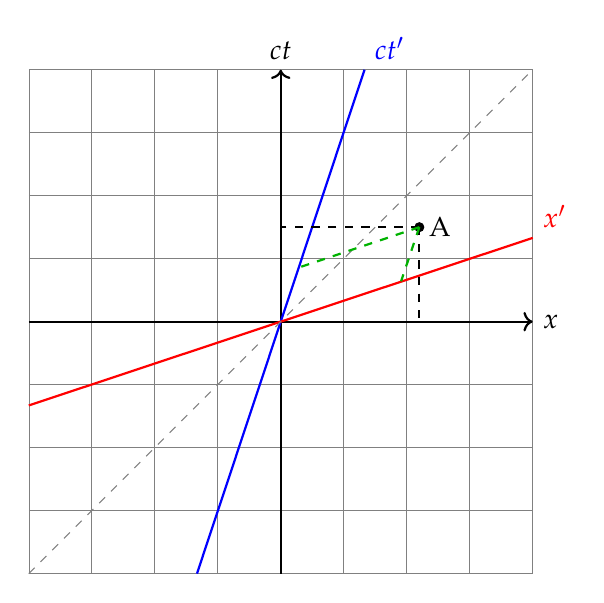
\begin{tikzpicture}[scale=0.8]
    % Grid
    \draw[step=1cm,gray,very thin] (-4,-4) grid (4,4);
    % Axes
    \draw[thick,->] (-4,0) -- (4,0) node[right] {$x$};
    \draw[thick,->] (0,-4) -- (0,4) node[above] {$ct$};
    
    % ct' and x' axes
    % Let v/c = 1/3 for ease.
    \draw[blue, thick] (-1.33, -4) -- (1.33, 4) node[above right] {$ct'$};
    \draw[red, thick] (-4, -1.33) -- (4, 1.33) node[above right] {$x'$};
    
    % Light lines
    \draw[dashed, gray] (-4,-4) -- (4,4);
    
    % Event A
    \filldraw[black] (2.2, 1.5) circle (2pt) node[right] {A};
    
    % Unprimed coordinates
    \draw[dashed, thick, black] (2.2, 1.5) -- (2.2, 0);
    \draw[dashed, thick, black] (2.2, 1.5) -- (0, 1.5);
    
    % Primed coordinates
    % Line parallel to ct' passing through A (slope 3)
    % ct - 1.5 = 3(x - 2.2) => ct = 3x - 6.6 + 1.5 = 3x - 5.1
    % Intersects x' axis (ct = 1/3 x):
    % 1/3 x = 3x - 5.1 => 8/3 x = 5.1 => x = 1.9125, ct = 0.6375
    \draw[dashed, thick, green!70!black] (2.2, 1.5) -- (1.91, 0.64);
    
    % Line parallel to x' passing through A (slope 1/3)
    % ct - 1.5 = 1/3(x - 2.2) => ct = 1/3 x - 0.733 + 1.5 = 1/3 x + 0.767
    % Intersects ct' axis (ct = 3x):
    % 3x = 1/3 x + 0.767 => 8/3 x = 0.767 => x = 0.287, ct = 0.863
    \draw[dashed, thick, green!70!black] (2.2, 1.5) -- (0.29, 0.86);
\end{tikzpicture}
\end{center}

\begin{exercise}[Exercise 11]
We have repeated below the figure you generated above. You concluded that the line joining the origin and event B corresponds to the $x'$ axis. We also indicated with the $x'$ label that the \textit{positive} $x'$ axis points up and to the right in the diagram. State precisely why we can conclude that this is the \textit{positive} $x'$ direction.
\end{exercise}
\begin{solution}
Light travels from the origin to Event B in the positive $x'$ direction before reflecting back. (The reflection at B reverses the direction of light to the negative $x'$ direction to return to the origin).
\end{solution}

\begin{exercise}[Exercise 12]
What do you think the primed axes will look like for an inertial frame moving in the \textit{negative} $x$ direction with speed $v$? Sketch them on the same spacetime diagram above and place the axis labels ($ct'$ and $x'$) at the \textit{positive} end of each coordinate axis.
\end{exercise}

\begin{exercise}[Exercise 13]
Now, to convince yourself that you did this correctly, go through the same sort of steps you used in the previous lecture:
\begin{enumerate}[label=(\alph*)]
    \item Draw the worldline of a clock that passes through the origin and moves to the left with speed $v$ to generate the $ct'$ axis. What is its slope?
    \item For the $x'$ axis, again draw the events A, B, C described above, in this new primed frame -- i.e., a light flash leaves A at position $x'=0$ and time $t'=-T$, travels to the right and arrives at B at $t'=0$, and then travels to the left and arrives back at $x'=0$ at time $t'=+T$.
\end{enumerate}
Did you put the label on the $x'$ axis at the correct end in the previous exercise?
\end{exercise}

% ==================== LECTURE 5 ====================
\chapter{Lorentz Transformations, Adding Velocities}

In the previous lecture, you developed a technique for finding the coordinates of \textit{arbitrary} events in \textit{arbitrary} inertial frames using spacetime diagrams. These are great for visualizing, but if you want the value of a quantity or a formula at the end of the calculation, then you probably want to use algebraic techniques instead. We are now going to deduce the formulae that transform $(ct, x)$ coordinates in one inertial frame into $(ct', x')$ coordinates in another inertial frame -- called the Lorentz transformations.

First, recall from problem 1 on Problem Set 0 that a transformation $T$ that maps a vector $\vec{r}$, say, to a vector $\vec{r}'$ ($T(\vec{r}) = \vec{r}'$) is a \textit{linear} transformation if it satisfies these two conditions:
\begin{enumerate}
    \item $T(\vec{r}_1 + \vec{r}_2) = T(\vec{r}_1) + T(\vec{r}_2)$ (additivity). In words, the transformation of the sum of two vectors is equal to the sum of their individual transformations.
    \item $T(a\vec{r}) = aT(\vec{r})$ (homogeneity). In words, multiplying a vector by a scalar $a$ before applying the transformation is equivalent to applying the transformation and then multiplying the result by the same scalar $a$.
\end{enumerate}

Note that this property follows from the above: $T(a\vec{r}_1 + b\vec{r}_2) = aT(\vec{r}_1) + bT(\vec{r}_2)$.

\begin{exercise}[Exercise 1]
Consider the tranformation describing a counterclockwise rotation of the $x$ and $y$ coordinate axes through an angle $\theta$ in two-dimensional $(x, y)$ space. A point with coordinates $(x, y)$ in the original system will be mapped onto the point with coordinates $(x', y')$ given by
\begin{align*}
    x' &= +\cos\theta \, x + \sin\theta \, y \\
    y' &= -\sin\theta \, x + \cos\theta \, y 
\end{align*}
Is this a linear transformation?
\end{exercise}
\begin{solution}
Yes. As a matrix: $\begin{bmatrix} x' \\ y' \end{bmatrix} = \begin{bmatrix} \cos\theta & \sin\theta \\ -\sin\theta & \cos\theta \end{bmatrix} \begin{bmatrix} x \\ y \end{bmatrix}$
\end{solution}

Note that we can also write this transformation as
\begin{align*}
    x' &= +a \, x + b \, y \\
    y' &= -b \, x + a \, y
\end{align*}
where $a = \cos\theta$ and $b = \sin\theta$, and that for this rotation transformation, $a^2 + b^2 = 1$.

A property of linear transformations in two dimensions that you may have encountered when working on Problem Set 0 is that \textbf{``grid lines'' that are parallel and evenly spaced remain parallel and evenly spaced, and the origin stays fixed, under a linear transformation.}\footnote{A grid line is a line along which a coordinate is constant. If you are already comfortable with matrices, or are learning about them in MATH 61, then you might enjoy this 3Blue1Brown video about linear transformations and grid lines: \url{https://www.youtube.com/watch?v=kYB8IZa5AuE}}

With spacetime diagrams, we showed geometrically that the transformation from the $(ct, x)$ coordinate system for one inertial frame to the $(ct', x')$ coordinate system for another inertial frame (traveling with respect to the first at velocity $v$) corresponds to one axis being rotated by angle $\theta$ and the other by angle $-\theta$, where $\theta$ depends on the velocity $v$.

\begin{exercise}[Quick Question]
For the spacetime transformation that we found geometrically, are ``grid lines'' in the $(ct', x')$ coordinate system parallel? So is the transformation from $(ct, x)$ to $(ct', x')$ linear?
\end{exercise}
\begin{solution}
Yes.
\end{solution}

You will now find the algebraic form of that transformation!

We can write the general transformation like this:
\begin{align}
    ct' &= A \, ct + B \, x \\
    x'  &= C \, ct + D \, x 
\end{align}
Our goal is to determine $A, B, C$, and $D$.

\begin{exercise}[Quick Exercise 2]
Why aren't there constant terms (e.g., $E$ in $ct' = Act + Bx + E$) in the linear system of equations?
\end{exercise}
\begin{solution}
Then it's not a linear transformation, and also it violates that $T(\vec{0}) = \vec{0}$.
\end{solution}

\begin{exercise}[Quick Exercise 3]
Are the origins of the coordinate systems the same under the above transformation?
\end{exercise}
\begin{solution}
Yes.
\end{solution}

\begin{exercise}[Quick Exercise 4]
Which of the quantities $A, B, C$, and $D$ is dimensionless (if any)?
\end{exercise}
\begin{solution}
All are.
\end{solution}

\begin{exercise}[Quick Exercise 5]
What quantities can $A, B, C$, and $D$ depend on?
\end{exercise}
\begin{solution}
$v/c$
\end{solution}

\begin{exercise}[Exercise 6]
Assume the $(ct', x')$ frames is moving with constant velocity $v$ with respect to the $(ct, x)$ frame. You will now use the following facts to reduce the number of unknowns:
\begin{enumerate}[label=(\alph*)]
    \item An object moving at velocity $v$ in the unprimed frame will be at rest in the primed frame. (This is the \textit{definition} of the primed frame!)
    \item Light travels at speed $c$ in both frames, whether traveling to the left or to the right. (Second postulate.)
\end{enumerate}
\end{exercise}

We'll guide you through this...

First, translate each statement into equations describing the relevant worldline, in each coordinate system.

For example, for statement (a), if we assume that the object is at position $x=x'=0$ at time $t=t'=0$, then the worldline of the object is described by the following equations in each of the coordinate systems:
\begin{align*}
    (ct, x) &\qquad (ct', x') \\
    x = vt &\iff x' = 0
\end{align*}

Next, plug appropriate values into the general linear transformation equations (repeated below for your convenience) to eliminate the variables $(x, ct, x', ct')$ and find relationships between the unknown coefficients. Finally, solve for $B, C$ and $D$ in terms of $A$. Let's get started!

\begin{tcolorbox}[colback=white, boxrule=1pt, arc=3pt, width=0.4\textwidth, center]
\begin{align*}
    ct' &= A \, ct + B \, x \tag{1} \\
    x'  &= C \, ct + D \, x \tag{2}
\end{align*}
\end{tcolorbox}

\textbf{(a) An object moving at velocity $v$ in the unprimed frame will be at rest in the primed frame.}
\begin{align*}
    x &= vt \iff x' = 0 \tag*{1st statement} \\
    \implies 0 &= C \, ct + D \, vt \tag*{plug expressions for $x$ and $x'$ into (2)} \\
    \implies -C \, ct &= D \, vt \implies D = -C \left(\frac{c}{v}\right) \tag*{solve for $D$}
\end{align*}

\textbf{(b) Light travels \textit{to the right} at speed $c$ in both frames.}
\begin{align*}
    x &= ct \iff x' = ct' \tag*{2nd statement for rightgoing light} \\
    (A+B)ct &= (C+D)ct \tag*{plug expression for $x$ into (1) and (2)} \\
    A+B &= C+D \implies A = -B + C + D \tag*{solve for $A$, for example}
\end{align*}

\textbf{(b) Light travels \textit{to the left} at speed $c$ in both frames.}
\begin{align*}
    x &= -ct \iff x' = -ct' \tag*{2nd statement for leftgoing light} \\
    (A-B)ct &= -(C-D)ct \tag*{plug expression for $x$ into (1) and (2)} \\
    A-B &= -C+D \implies A = B - C + D \tag*{solve for $A$, for example}
\end{align*}

We now have three equations in four unknowns; let's solve for $D, C$, and $B$ in terms of $A$:
\begin{align*}
    \begin{cases}
    D &= - \frac{c}{v} C \\
    A &= -B + C + D \\
    A &= +B - C + D 
    \end{cases}
    \implies
    \begin{cases}
    D &= A \\
    C &= -\frac{v}{c} A \\
    B &= -\frac{v}{c} A
    \end{cases}
\end{align*}

After applying these three independent constraints, the number of unknowns is reduced to just one. In terms of $A$ (fill in the missing coefficients),
\begin{align}
    ct' &= A \left( ct - \frac{v}{c} \, x \right) \tag{3} \\
    x'  &= A \left( x - \frac{v}{c} \, ct \right) \tag{4}
\end{align}

Lastly, we need to determine $A$. There are a few ways to do this; the simplest is to invoke time dilation, which, as we recall, we derived using the postulates.

\begin{exercise}[Exercise 7]
If a clock is at rest at the origin in the unprimed frame (i.e., at $x=0$) and ticks at time $t$, then it ticks at time $t' = \gamma t$ in the primed frame. Plugging these into equation (3), we get $A = \gamma$.
\end{exercise}

Finally, we arrive at the \textbf{Lorentz transformation equations}:
\begin{align*}
    ct' &= \gamma \left( ct - \frac{v}{c} \, x \right) \\
    x'  &= \gamma \left( x - \frac{v}{c} \, ct \right)
\end{align*}

where as usual $\gamma = \frac{1}{\sqrt{1-v^2/c^2}}$.

\begin{exercise}[Quick Check]
Are the coefficients dimensionless, as expected?
\end{exercise}

The change of coordinates implemented by the Lorentz transformation is called a \textbf{boost}.\footnote{Boosting is different from \textit{accelerating}!} It is common to designate the velocity of the boost by the dimensionless ratio
\[ \beta = \frac{\text{velocity of frame}}{c}. \tag*{(\text{Greek letter \textit{beta}})} \]

\begin{exercise}[Quick Question]
What are the bounds on $\beta$?
\end{exercise}
\begin{solution}
$|\beta| \le 1$.
\end{solution}

Using $\beta$ for the boost will free us up to use $v$ for other velocities, which will be important soon. Note that we can also write $\gamma$ in terms of $\beta$:
\[ \gamma = \frac{1}{\sqrt{1-v^2/c^2}} = \frac{1}{\sqrt{1-\beta^2}} \]

In terms of the boost $\beta$, the Lorentz transformations are written as
\begin{align*}
    ct' &= \gamma (ct - \beta x), \\
    x'  &= \gamma (x - \beta ct).
\end{align*}

It is also useful to invert these equations -- i.e., solve for $(ct, x)$ in terms of $(ct', x')$.

\begin{exercise}[Exercise 8]
Write down the equations for the inverse Lorentz transformations. Do it ``the easy way'' (using physical reasoning).
\end{exercise}
\begin{solution}
\begin{align*}
    ct &= \gamma (ct' + \beta x') \\
    x  &= \gamma (x' + \beta ct')
\end{align*}
\end{solution}

(We recommend that you try it the ``hard way'', by algebraically inverting the equations, on your own. It takes a bit of work to get it into the final form!)

\begin{exercise}[Exercise 9]
Consider events 1 and 2 with coordinates $(ct_1, x_1)$ and $(ct_2, x_2)$ in one inertial frame, and coordinates $(ct_1', x_1')$ and $(ct_2', x_2')$ in another inertial frame. Define the time and space intervals between events 1 and 2 in each frame:
\begin{align*}
    \Delta t &= t_1 - t_2, \quad \Delta x = x_1 - x_2, \\
    \Delta t' &= t_1' - t_2', \quad \Delta x' = x_1' - x_2'.
\end{align*}
Do the Lorentz transformations apply to these coordinate \textit{differences} (i.e., intervals of space and time) as well as to the coordinates themselves? That is, do $c\Delta t$ and $\Delta x$ transform in the same way as $ct$ and $x$, as in the following equations?
\begin{align*}
    c\Delta t' &= \gamma (c\Delta t - \beta\Delta x) \\
    \Delta x' &= \gamma (\Delta x - \beta c\Delta t)
\end{align*}
Justify your response with a precise statement.
\end{exercise}
\begin{solution}
Yeah. The transformations are linear.
\end{solution}

We will frequently use this ``interval'' form of the Lorentz transformation equations, including in the next section.

\section{Velocity Addition Rule}

\begin{itemize}
    \item Suppose an object is moving with velocity $v$ (in the $x$ direction) in an inertial frame described with unprimed coordinates.
    \item Another inertial frame, described with primed coordinates, is related to the unprimed frame by a boost $\beta$ in the $x$ direction -- i.e., the primed frame is moving with velocity $\beta c$ according to an inertial observer in the unprimed frame.
\end{itemize}

\begin{exercise}[Quick Exercise 10]
Draw a sketch of the situation described above. Then write down an expression for the \textit{Newtonian expectation} for $v'$, the velocity of the object as observed in the primed frame, in terms of $v$ and $\beta c$. Check that your signs are correct by considering two special cases: (i) $\beta c = 0$ and (ii) $v = 0$. Do you get the expected result for each case?
\end{exercise}
\begin{solution}
\textit{(Sketch showing an unprimed observer seeing an object moving at $v$, while a primed observer moves right at $\beta c$.)} \\
Newtonian expectation: $v' = v - \beta c$
\end{solution}

\begin{exercise}[Exercise 11]
Now find the \textit{relativistic} transformation rule for velocity under a boost by $\beta$. In other words, suppose that an object moves at velocity $v = \frac{\Delta x}{\Delta t}$ in the unprimed frame. Find $v' = \frac{\Delta x'}{\Delta t'}$. (Remember that $\beta$ is associated with the boost of the primed frame, while $v$ is the velocity of the object as observed in the unprimed frame. $\beta \neq v/c$ here!)
\end{exercise}
\begin{solution}
\begin{align*}
    v' &= \frac{\Delta x'}{\Delta t'} = \frac{\gamma(\Delta x - \beta c \Delta t)}{\gamma(\Delta t - \beta \Delta x / c)} \qquad \text{use } \Delta x = v\Delta t \\
       &= \frac{v\Delta t - \beta c \Delta t}{\Delta t - \beta v \Delta t / c} \\
       &= \frac{v - \beta c}{1 - \frac{\beta v}{c}} = \frac{v_1 - v_2}{1 - \frac{v_1 v_2}{c^2}}
\end{align*}
\end{solution}

In physics situations, we often talk about \textit{adding} velocities; for example, an object is thrown at velocity $u$ relative to a train that is moving at velocity $v$ with respect to the observer. ``Adding'' velocity $u$ to velocity $v$ is equivalent to boosting the (primed) observer's frame by $\beta = -v/c$. In other words, set $\beta c = -v$ in the equation you derived above to find that the resultant velocity is
\[ u \oplus v = \frac{u + v}{1 + \frac{uv}{c^2}} \]
where the symbol $\oplus$ is defined to mean `add the velocities relativistically' according to this rule.

\begin{exercise}[Exercise 12]
Determine the approximate or exact result of relativistic velocity addition for the following two cases, and explain the physical interpretation of each result.
\begin{itemize}
    \item $u \oplus v$ when $u, v \ll c$.
    \item $u \oplus v$ when $v = c$.
\end{itemize}
\end{exercise}
\begin{solution}
\begin{itemize}
    \item $u \oplus v \approx u + v$ (reduces to Galilean/Newtonian velocity addition)
    \item $u \oplus c = c$ (the speed of light is $c$ in all frames!)
\end{itemize}
\end{solution}

% ==================== LECTURE 6 ====================
\chapter{Spacetime Interval \& Causality}

\section{Causality}

Two events are described as ``causally connected'' if they must occur in a certain order in time because one causes the other. For example, if someone sitting on a chair presses a button on a remote control (RC) unit to change a channel on a television, the two events (press the button $\Rightarrow$ channel changes) must happen in that order; the channel cannot change before the button is pressed!

\begin{exercise}[Quick question 1]
What is the ``causal influence'' between these events? How fast does it travel?
\end{exercise}
\begin{solution}
The causal influence is the signal from the remote. It travels at the speed of light. The remote click causes the TV to flash.
\end{solution}

Now, suppose someone \textit{claims} to have invented the FTc RC (``Faster Than $c$'' RC) -- an RC unit that sends a new type of signal that travels \textit{faster than light} to your TV -- say, at speed $5c$. Is an FTc RC consistent with Einstein's postulates? Let's find out!

Assume that the RC unit is at $x=0$ and the TV is at $x = +5$ nano-light-seconds ($+5\, c\,\text{ns}$).

\begin{exercise}[Quick question 2]
Is 5 nano-light-seconds a physically reasonable distance?
\end{exercise}
\begin{solution}
Yes, it's about 5 feet.
\end{solution}

You will now work on your whiteboard with your group to discover the fundamental flaw in the ``faster than light'' claim...

\begin{exercise}[Exercise 1]
Draw a spacetime diagram with the unprimed coordinates ($ct$ and $x$) corresponding to the TV viewer's reference frame.
\begin{enumerate}[label=(\alph*)]
    \item Draw the worldlines for the FTc RC unit and for the receiver located in the TV. Include a scale on the axes.
    \item Now draw the worldline for the faster-than-light ($v=5c$) signal, assuming that the signal leaves the RC unit at $t=0$. (What is its slope?) Use the labels \textbf{P} and \textbf{Q} to indicate the locations of these two events:
    
    P = the faster-than-light signal leaves the transmitter;
    
    Q = the faster-than-light signal arrives at the receiver.
    \item Now just \textit{suppose} an inertial observer in a ``primed'' inertial frame is moving in the $+x$ direction with velocity $\beta c = +\frac{2}{5} c$ with respect to the unprimed frame -- i.e., the inertial observer in the primed frame is traveling at speed \textit{less} than $c$ in the unprimed frame.
    
    Draw the $ct'$ and $x'$ coordinate axes for this observer's inertial frame, assuming a common origin for the primed and unprimed frames.
    \item Indicate the $ct'$ coordinates of events \textbf{P} and \textbf{Q} on your diagram -- i.e., the times at which the `primed' observer observes the events.
    
    Which event happens first in the primed reference frame -- event \textbf{P} or event \textbf{Q}?
    
    Is your result consistent with Einstein's postulates? Explain.
\end{enumerate}
\end{exercise}

\begin{center}
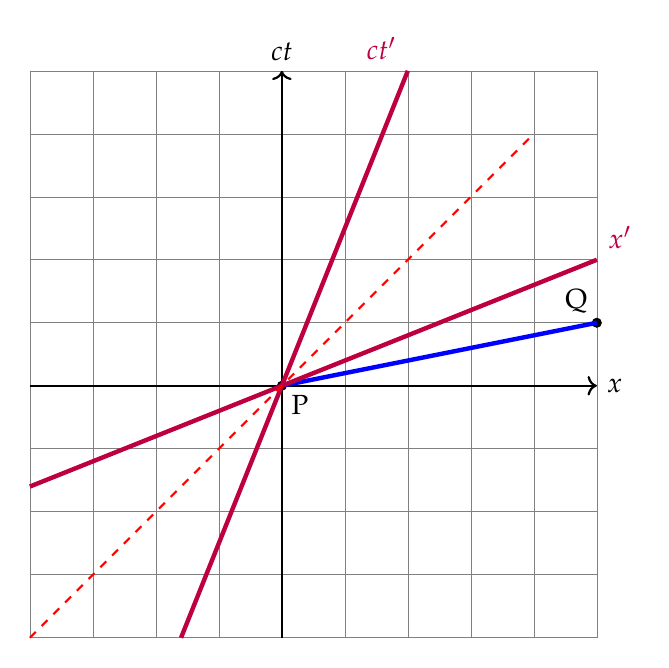
\begin{tikzpicture}[scale=0.8]
    % Grid
    \draw[step=1cm,gray,very thin] (-4,-4) grid (5,5);
    % Axes
    \draw[thick,->] (-4,0) -- (5,0) node[right] {$x$};
    \draw[thick,->] (0,-4) -- (0,5) node[above] {$ct$};
    
    % Event P at origin
    \filldraw[black] (0,0) circle (2pt) node[below right] {P};
    
    % Event Q at x=5, t=1 (since v=5c => x=5c*t => ct = x/5 = 1)
    \filldraw[black] (5,1) circle (2pt) node[above left] {Q};
    
    % Worldline of signal P->Q
    \draw[ultra thick, blue] (0,0) -- (5,1);
    
    % Primed axes for beta = 2/5.
    % x' axis has slope beta = 2/5
    \draw[ultra thick, purple] (-4, -1.6) -- (5, 2) node[above right] {$x'$};
    
    % ct' axis has slope 1/beta = 5/2 = 2.5
    \draw[ultra thick, purple] (-1.6, -4) -- (2, 5) node[above left] {$ct'$};
    
    % Light line for reference
    \draw[dashed, red, thick] (-4,-4) -- (4,4);
\end{tikzpicture}
\end{center}

\begin{solution}
For (d): Event P is at the origin, so its $ct'$ coordinate is $0$.
Event Q has a positive $x$ coordinate but is \textit{below} the $x'$ axis in the spacetime diagram. Therefore, its $ct'$ coordinate is \textit{negative}! 

In the primed frame, Q happens \textit{before} P. The effect precedes the cause! This violates causality.
\end{solution}

\textbf{Conclusion:} No signal (or information) can travel faster than the speed of light in vacuum!

\section{Spacetime Interval}

In 2D or 3D space (\textit{not} spacetime!), rotations \textit{preserve the distance between two points}. In fact, this is one of the defining properties of rotations -- they preserve distances.
\begin{itemize}
    \item If you would like to see precisely why this is mathematically true, see the Appendix at the end of this lecture \textit{after} today's lesson. Reviewing this proof that \textit{rotations} preserve the distance between two points in \textit{space} can be useful to compare and contrast with `boosts' between inertial frames in \textit{spacetime}, which we will tackle now.
\end{itemize}

Here is the question we will now address:
\begin{itemize}
    \item Is there any interval in spacetime (i.e., any ``distance between \textbf{events}'') that is preserved under boosts (Lorentz transformations)?
\end{itemize}

In other words, is there any interval between a pair of events for which all inertial observers would agree upon the value? First, recall the Lorentz transformation equations expressed in terms of coordinate differences between events 1 and 2:
\begin{align*}
    c\Delta t' &= \gamma(c\Delta t - \beta \Delta x), \\
    \Delta x'  &= \gamma(\Delta x - \beta c\Delta t),
\end{align*}
where $\Delta t = t_2 - t_1, \; \Delta x = x_2 - x_1$, $\Delta t' = t_2' - t_1', \; \Delta x' = x_2' - x_1'$, $\beta \equiv \frac{v_{\text{frame}}}{c}, \; \gamma = (1 - \beta^2)^{-1/2}$.

\begin{exercise}[Exercise 2]
Let's \textit{define} a \textbf{spacetime interval} between two events as
\[ (\Delta s)^2 \equiv (c\Delta t)^2 - (\Delta x)^2. \]
Is this a \textit{useful} quantity? Let's see.
\begin{enumerate}[label=(\alph*)]
    \item Does $(\Delta s')^2 = (\Delta s)^2$? That is, use the Lorentz transformation equations to check whether $(c\Delta t')^2 - (\Delta x')^2 = (c\Delta t)^2 - (\Delta x)^2$.
    \item Is the spacetime interval always positive? If not, describe two events for which the spacetime interval is negative.
    \item Under what condition is the spacetime interval equal to 0? Interpret this condition.
\end{enumerate}
\end{exercise}

\begin{solution}
(a)
\begin{align*}
    (c\Delta t')^2 - (\Delta x')^2 &= \gamma^2(c\Delta t - \beta \Delta x)^2 - \gamma^2(\Delta x - \beta c\Delta t)^2 \\
    &= \gamma^2 \left( c^2\Delta t^2 - 2\beta c\Delta x\Delta t + \beta^2\Delta x^2 - \Delta x^2 + 2\beta c\Delta x\Delta t - \beta^2 c^2\Delta t^2 \right) \\
    &= \gamma^2 \left( c^2\Delta t^2 - \Delta x^2 \right) (1-\beta^2) \\
    &= (c\Delta t)^2 - (\Delta x)^2 \qquad \text{since } \gamma^2(1-\beta^2) = 1
\end{align*}
(b) No; if $(\Delta x)^2 > (c\Delta t)^2$, the interval is negative. \\
(c) When $\Delta x = c\Delta t$, i.e., along a light ray.
\end{solution}

\textbf{Summary:}
\begin{enumerate}
    \item Based on the above exercise, we conclude that the spacetime interval is \textbf{invariant} -- it doesn't change when we change inertial reference frames.
    
    In other words, \textit{all inertial observers agree on the spacetime interval between two events!}
    \item The difference between 2D space $(x, y)$ and spacetime $(x, ct)$, then, is `just' the minus sign in how we calculate the interval between points and events, respectively.
    \item Note that the interval is $(\Delta s)^2$ (also written $\Delta s^2$), not $\sqrt{\Delta s^2}$ (or ``$\Delta s$''), which may not even be a real number...
\end{enumerate}

We'll now define three categories of pairs of events:

\begin{itemize}
    \item Two events are \textbf{lightlike separated} if $(\Delta x)^2 = (c\Delta t)^2 \implies \Delta s^2 = 0$
    -- i.e., the two terms are \textbf{equal}.
    
    \item Two events are \textbf{timelike separated} if $(c\Delta t)^2 > (\Delta x)^2 \implies \Delta s^2 > 0$
    -- i.e., the square of the \textbf{time} interval is larger than the square of the space interval.
    
    \item Two events are \textbf{spacelike separated} if $(\Delta x)^2 > (c\Delta t)^2 \implies \Delta s^2 < 0$
    -- i.e., the square of the \textbf{space} interval is larger than the square of the time interval.
\end{itemize}

\begin{exercise}[Exercise 3]
Consider two events that lie along the worldline of an object moving with constant velocity $v < c$. Are the two events lightlike, timelike, or spacelike separated?
\end{exercise}
\begin{solution}
Timelike.
\end{solution}

\begin{exercise}[Exercise 4]
Draw a spacetime diagram on your whiteboard; as usual, include worldlines for light through the origin. Draw an event \textbf{P} at the origin ($x=ct=0$). Now, consider the following descriptions of two different categories of pairs of events, \textbf{P} and $\mathbf{Q_{\text{I}}}$, and \textbf{P} and $\mathbf{Q_{\text{II}}}$.
\begin{itemize}
    \item For each category, circle whether the events are timelike or spacelike separated.
    \item Then draw on your spacetime diagram several examples of an event \textbf{Q}, such that \textbf{P} and \textbf{Q} satisfy the description (with \textbf{P} at the origin). Label them $\mathbf{Q_{\text{I}}}$ or $\mathbf{Q_{\text{II}}}$.
\end{itemize}

\textbf{I.} We can find a frame in which \textbf{P} and $\mathbf{Q_{\text{I}}}$ occur at the \textit{same time}. In this frame, the magnitude of the spacetime interval is the \textit{distance}-squared between the events. 
(Timelike separated? \textbf{Spacelike separated?})

\textbf{II.} We can find a frame in which \textbf{P} and $\mathbf{Q_{\text{II}}}$ occur at the \textit{same place}. In this frame, the magnitude of the spacetime interval is the \textit{time}-squared between the events. 
(\textbf{Timelike separated?} Spacelike separated?)
\end{exercise}

\begin{center}
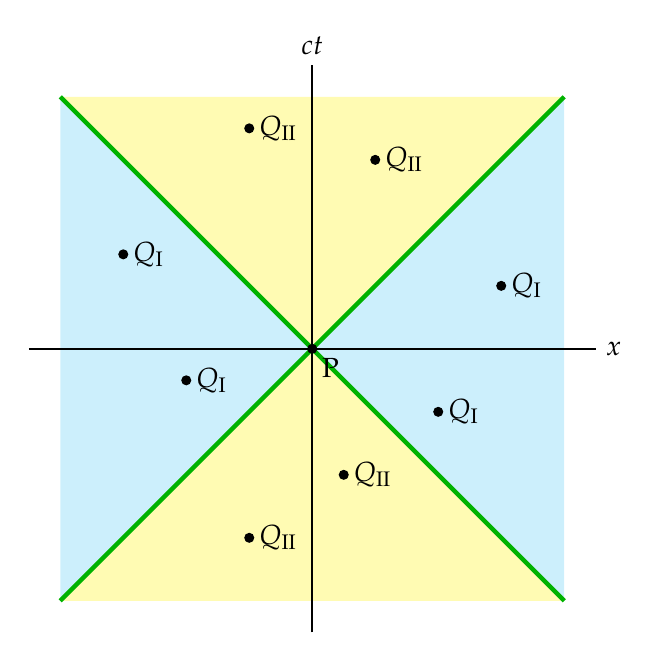
\begin{tikzpicture}[scale=0.8]
    % Light cones (regions)
    \fill[yellow!30] (-4,4) -- (0,0) -- (4,4) -- cycle;
    \fill[yellow!30] (-4,-4) -- (0,0) -- (4,-4) -- cycle;
    \fill[cyan!20] (-4,4) -- (0,0) -- (-4,-4) -- cycle;
    \fill[cyan!20] (4,4) -- (0,0) -- (4,-4) -- cycle;

    % Axes
    \draw[thick] (-4.5,0) -- (4.5,0) node[right] {$x$};
    \draw[thick] (0,-4.5) -- (0,4.5) node[above] {$ct$};
    
    % Light lines
    \draw[ultra thick, green!70!black] (-4,-4) -- (4,4);
    \draw[ultra thick, green!70!black] (-4,4) -- (4,-4);
    
    % Event P at origin
    \filldraw[black] (0,0) circle (2pt) node[below right] {P};
    
    % Q_II points (Timelike)
    \filldraw[black] (1,3) circle (2pt) node[right] {$Q_{\text{II}}$};
    \filldraw[black] (-1,3.5) circle (2pt) node[right] {$Q_{\text{II}}$};
    \filldraw[black] (0.5,-2) circle (2pt) node[right] {$Q_{\text{II}}$};
    \filldraw[black] (-1,-3) circle (2pt) node[right] {$Q_{\text{II}}$};
    
    % Q_I points (Spacelike)
    \filldraw[black] (3,1) circle (2pt) node[right] {$Q_{\text{I}}$};
    \filldraw[black] (2,-1) circle (2pt) node[right] {$Q_{\text{I}}$};
    \filldraw[black] (-3,1.5) circle (2pt) node[right] {$Q_{\text{I}}$};
    \filldraw[black] (-2,-0.5) circle (2pt) node[right] {$Q_{\text{I}}$};
\end{tikzpicture}
\end{center}

Now indicate on your spacetime diagram the \textit{regions} of spacetime in which \textbf{Q} can lie (relative to \textbf{P} at the origin) for the three categories we defined:
\begin{itemize}
    \item \colorbox{yellow!30}{Timelike separated from \textbf{P} (i.e., $(\Delta s)^2 > 0$).}
    \item \colorbox{cyan!20}{Spacelike separation from \textbf{P} (i.e., $(\Delta s)^2 < 0$).}
    \item \colorbox{green!30}{Lightlike separation from \textbf{P} (i.e., $(\Delta s)^2 = 0$).}
\end{itemize}

\textbf{Things to note:}
\begin{itemize}
    \item Because the value of the spacetime interval $\Delta s^2$ is \textit{inertial-frame-independent} no matter what its sign, all inertial observers will agree as to whether the interval between a given pair of events is timelike, lightlike, or spacelike.
    \item The three regions distinguish those events that can be \textit{causally} connected to \textbf{P} from those that cannot.
\end{itemize}

\begin{exercise}[Quick Question]
Which events \textbf{Q} \textit{could} be causally connected to \textbf{P} -- those that lie in the timelike region? the lightlike line? the spacelike region?
\end{exercise}
\begin{solution}
The timelike region and the lightlike line.
\end{solution}

\textbf{More things to note for timelike-separated events:}
\begin{itemize}
    \item The temporal order of events is preserved in all inertial frames for \textit{timelike}-separated pairs of events. (Try showing this with a timelike-separated pair of events on a spacetime diagram.)
    \item Therefore, all events in the upper timelike region will occur \textit{after} \textbf{P} in \textit{every} frame (and thus could be caused by P), and all events in the lower timelike region will occur \textit{before} \textbf{P} in every frame (and thus could \textit{cause} P).
\end{itemize}

\begin{exercise}[Exercise 5]
The \textit{boundaries} between the regions described above are worldlines of light. Describe the boundaries between these regions if we consider \textit{two} spatial dimensions ($x$ and $y$) instead of one.
\end{exercise}
\begin{solution}
$t^2 = x^2 + y^2$ (a cone). This is the spatial distance from the origin squared.
\end{solution}

\section{Optional material ... for now: Comparison of invariant quantities for rotations in 2D space \& Lorentz transformations in spacetime.}

First let's look at precisely why rotations preserve the distance between two points so that we can compare and contrast with spacetime.

Let $(x, y)$ and $(x', y')$ be the spatial coordinates of a point in the original and rotated frames. Since rotation is a linear transformation, the transformation we wrote down in the previous lecture applies to coordinate \textit{intervals} as well as the coordinates themselves:
\begin{align*}
    \Delta x' &= +\cos\theta \, \Delta x + \sin\theta \, \Delta y \\
    \Delta y' &= -\sin\theta \, \Delta x + \cos\theta \, \Delta y 
\end{align*}

If we define $\Delta d^2 = \Delta x^2 + \Delta y^2$ and $\Delta d'^2 = \Delta x'^2 + \Delta y'^2$ to be the squared distance between two points in the plane as measured in the original and rotated frames, respectively, then, in Euclidean geometry,
\begin{align*}
    (\Delta d')^2 &= (\Delta x')^2 + (\Delta y')^2 \\
    &= (\cos\theta \, \Delta x + \sin\theta \, \Delta y)^2 + (-\sin\theta \, \Delta x + \cos\theta \, \Delta y)^2 \tag*{cross terms cancel} \\
    &= (\cos^2\theta + \sin^2\theta)\Delta x^2 + (\sin^2\theta + \cos^2\theta)\Delta y^2 \tag*{use trig identity} \\
    &= (\Delta d)^2
\end{align*}
$\implies \Delta d^2 = \Delta x^2 + \Delta y^2$ is invariant under rotations in 2D space.

\begin{itemize}
    \item In the above derivation, we used the trig identity $\cos^2\theta + \sin^2\theta = 1$ to show that the space-space quantity $\Delta x^2 + \Delta y^2$ is invariant under rotation.
    \item In the optional (for now) material at the end of Lecture 5, we wrote the Lorentz transformation equations in terms of the \textit{hyperbolic} trig functions:
\begin{align*}
    ct' &= +\cosh w \, ct - \sinh w \, x \\
    x'  &= -\sinh w \, ct + \cosh w \, x 
\end{align*}
You might recognize that we could use a similar derivation for spacetime intervals to show that $(\Delta s)^2 \equiv (c\Delta t)^2 - (\Delta x)^2$ is invariant under Lorentz transformations. However, in this case we would use the corresponding identity for hyperbolic trig functions:
\[ \cosh^2 w - \sinh^2 w = 1. \]
\end{itemize}

\section{Boosts vs. Rotations}

We saw from constructing axes on spacetime diagrams (as compared with space-space diagrams) that boosts have similarities, but also marked differences, from rotations. Compare the transformation equations written in a slightly different form:

\begin{minipage}[t]{0.45\textwidth}
\begin{center}
    Boost by $\beta$
    \begin{align*}
        ct' &= +\gamma \, ct - \beta\gamma \, x \\
        x'  &= -\beta\gamma \, ct + \gamma \, x
    \end{align*}
\end{center}
\end{minipage}
\begin{minipage}[t]{0.45\textwidth}
\begin{center}
    Rotation by $\theta$
    \begin{align*}
        x' &= +\cos\theta \, x + \sin\theta \, y \\
        y' &= -\sin\theta \, x + \cos\theta \, y
    \end{align*}
\end{center}
\end{minipage}

\begin{exercise}[Discuss]
What are some similarities and differences between the two transformations?
\end{exercise}

\subsection{Optional material ... for now.}

One difference is that the rotations involve trig functions, and the boosts don't. Or do they? How can we check?

Well, for all values of $\theta$, $\sin^2\theta + \cos^2\theta = 1$, and conversely if $a^2 + b^2 = 1$ then $a = \cos\theta$ and $b = \sin\theta$ for some $\theta$. So if $\gamma^2 + (\beta\gamma)^2 = 1$ then we can write the boosts in terms of trig functions as well.

\begin{exercise}[Exercise 13]
Show that $\gamma^2 + (\beta\gamma)^2 \neq 1$.
\end{exercise}

Hopefully you noticed that a slight modification \textit{would} work:

\begin{exercise}[Exercise 14]
Now show that $\gamma^2 - (\beta\gamma)^2 = 1$.
\end{exercise}

There are ``trig-like'' functions that satisfy this relation; they are called the \textit{hyperbolic trig functions}. Here's the identity: $\cosh^2 w - \sinh^2 w = 1$. In other words, there exists a `hyperbolic angle' $w$ (this notation is not very standard) such that $\gamma = \cosh w$, $\beta\gamma = \sinh w$, and the Lorentz transformations are
\begin{align*}
    ct' &= \cosh w \, ct - \sinh w \, x \\
    x'  &= -\sinh w \, ct + \cosh w \, x 
\end{align*}
a.k.a. a \textit{hyperbolic rotation}.

If you are unfamiliar with hyperbolic trig functions, don't worry -- we won't be using them directly very much at all. The intent of this section was to show you that boosts and rotations are mathematically quite similar, but with two important differences: a minus sign, and hyperbolic instead of circular trig functions. We'll return to the significance of the hyperbolic feature later...

% ==================== LECTURE 7 ====================
\chapter{Four-Vectors, Dynamics}

\begin{exercise}[Exercise 1]
Precisely and concisely define these two words (as typically used in physics). Give a couple of examples of each.
\begin{itemize}
    \item Conserved:
    \item Invariant:
\end{itemize}
\end{exercise}
\begin{solution}
\begin{itemize}
    \item \textbf{Conserved:} Constant in time. Energy is conserved in a certain frame, but not preserved across frames.
    \item \textbf{Invariant:} Constant in spacetime. Invariant in every frame. The same in every Lorentz transformation.
\end{itemize}
\end{solution}

\section{From Kinematics to Dynamics}

So far, everything we've learned about special relativity has been \textit{kinematics} -- describing the motion of objects through space and time, without saying anything about how or why the motion changes.

Newton handled \textit{dynamics} through his three laws. Indeed, in Newtonian mechanics, conservation of total momentum ($\vec{p}$) and total energy in an isolated system follows from Newton's Laws. We will see that the definitions of (conserved) momentum and energy must be modified in relativity, due to the specific way in which velocity transforms between inertial frames.

Consider an object of mass $2m$, at rest in the ``unprimed'' inertial frame. It explodes into two halves, labeled 1 and 2 (each with mass $m$), moving in opposite directions at velocities $v_0$ and $-v_0$ (in one dimension), with momenta $mv_0$ and $-mv_0$. The total momentum is conserved in this frame -- i.e., it is 0 before and after the explosion.

\begin{center}
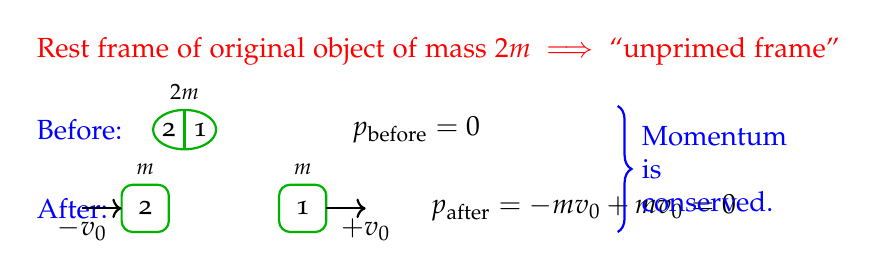
\begin{tikzpicture}[scale=1]
    \node[anchor=west, text=red] at (-1, 1.5) {Rest frame of original object of mass $2m \implies$ ``unprimed frame''};
    
    % Before
    \node[anchor=west, text=blue] at (-1, 0.5) {Before:};
    \draw[green!70!black, thick] (1, 0.5) ellipse (0.4 and 0.25);
    \node at (0.8, 0.5) {2}; \node at (1.2, 0.5) {1};
    \draw[green!70!black, thick] (1, 0.75) -- (1, 0.25);
    \node[above] at (1, 0.75) {\footnotesize $2m$};
    
    \node[anchor=west] at (3, 0.5) {$p_{\text{before}} = 0$};
    
    % After
    \node[anchor=west, text=blue] at (-1, -0.5) {After:};
    \draw[green!70!black, thick, rounded corners] (0.2,-0.2) rectangle (0.8, -0.8);
    \node at (0.5, -0.5) {2};
    \node[above] at (0.5, -0.2) {\footnotesize $m$};
    \draw[thick, <-] (0.2, -0.5) -- (-0.3, -0.5) node[below] {$-v_0$};
    
    \draw[green!70!black, thick, rounded corners] (2.2,-0.2) rectangle (2.8, -0.8);
    \node at (2.5, -0.5) {1};
    \node[above] at (2.5, -0.2) {\footnotesize $m$};
    \draw[thick, ->] (2.8, -0.5) -- (3.3, -0.5) node[below] {$+v_0$};
    
    \node[anchor=west] at (4, -0.5) {$p_{\text{after}} = -mv_0 + mv_0 = 0$};
    
    % Bracket
    \draw[thick, blue, decorate, decoration={brace, amplitude=5pt}] (6.5, 0.8) -- (6.5, -0.8) node[midway, right, align=left, xshift=5pt] {Momentum \\ is \\ conserved.};
\end{tikzpicture}
\end{center}

In Newtonian mechanics, the total momentum of this system is conserved in a ``boosted'' inertial frame as well -- e.g., a frame in which the object is moving with velocity $u$.

\begin{center}
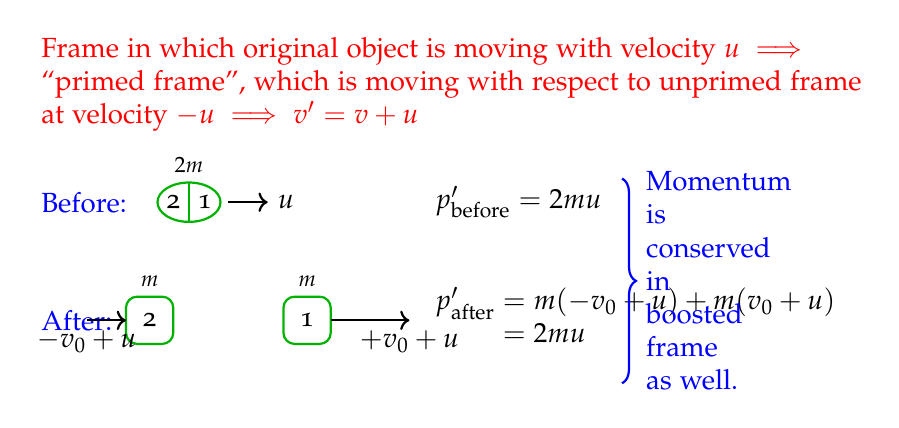
\begin{tikzpicture}[scale=1]
    \node[anchor=west, text=red, align=left] at (-1, 2) {Frame in which original object is moving with velocity $u \implies$ \\ ``primed frame'', which is moving with respect to unprimed frame \\ at velocity $-u \implies v' = v + u$};
    
    % Before
    \node[anchor=west, text=blue] at (-1, 0.5) {Before:};
    \draw[green!70!black, thick] (1, 0.5) ellipse (0.4 and 0.25);
    \node at (0.8, 0.5) {2}; \node at (1.2, 0.5) {1};
    \draw[green!70!black, thick] (1, 0.75) -- (1, 0.25);
    \node[above] at (1, 0.75) {\footnotesize $2m$};
    \draw[thick, ->] (1.5, 0.5) -- (2.0, 0.5) node[right] {$u$};
    
    \node[anchor=west] at (4, 0.5) {$p'_{\text{before}} = 2mu$};
    
    % After
    \node[anchor=west, text=blue] at (-1, -1) {After:};
    \draw[green!70!black, thick, rounded corners] (0.2,-0.7) rectangle (0.8, -1.3);
    \node at (0.5, -1) {2};
    \node[above] at (0.5, -0.7) {\footnotesize $m$};
    \draw[thick, <-] (0.2, -1) -- (-0.3, -1) node[below] {$-v_0+u$};
    
    \draw[green!70!black, thick, rounded corners] (2.2,-0.7) rectangle (2.8, -1.3);
    \node at (2.5, -1) {1};
    \node[above] at (2.5, -0.7) {\footnotesize $m$};
    \draw[thick, ->] (2.8, -1) -- (3.8, -1) node[below] {$+v_0+u$};
    
    \node[anchor=west, align=left] at (4, -1) {$p'_{\text{after}} = m(-v_0+u) + m(v_0+u)$ \\ $\phantom{p'_{\text{after}}} = 2mu$};
    
    % Bracket
    \draw[thick, blue, decorate, decoration={brace, amplitude=5pt}] (6.5, 0.8) -- (6.5, -1.8) node[midway, right, align=left, xshift=5pt] {Momentum \\ is \\ conserved \\ in \\ boosted \\ frame \\ as well.};
\end{tikzpicture}
\end{center}

Why is total momentum conserved in the boosted frame? Because when we move to a new inertial frame, \textbf{the transformation of the sum of momenta} is the same as \textbf{the sum of the transformed momenta} when momentum is defined as $p = mv$ and velocity transforms as $v' = v + u$:
\[ \text{If } p = mv, \text{ then } p' = mv' = m(v + u) = mv + mu. \]
In other words, it's because momentum depends linearly on velocity and the velocities just ``add'' under the transformation to a new frame.

Now let's consider the usual definition of momentum in Newtonian mechanics, $p_N \equiv mv$, but combine it with the \textbf{relativistic} velocity transformation equation that we derived near the end of Lecture 5:
\begin{equation}
v' = \frac{v - \beta c}{1 - \beta v/c}, \quad \text{where } \beta = v_{\text{frame}}/c.
\end{equation}
(In the above example, $u = -\beta c$.)

\begin{exercise}[Exercise 2]
Do you expect that total Newtonian momentum, defined as $p_N \equiv mv$, will be a conserved quantity during the process illustrated on the previous page, if the velocity $v$ transforms as in equation (1)?
\end{exercise}
\begin{solution}
Nah.
\end{solution}

\textbf{Summary}
\begin{itemize}
    \item The basic failure of \textit{Newtonian} momentum conservation under a Lorentz transformation of space and time arises because \textbf{the transformation of the sum of momenta} is different from \textbf{the sum of the transformed momenta} when momentum is defined as $p = mv$ with $v$ transformed as in equation (1).
    \item We can express this as the following equation, where $\Lambda$ represents the non-linear relativistic transformation for \textit{velocities}:
    \[ \Lambda(mv_1 + mv_2) \neq \Lambda(mv_1) + \Lambda(mv_2). \tag{\textcolor{blue}{bad}} \]
    \item The transformation equation for velocity $v$ is the culprit because $v$ and $\beta c$ appears (linearly) in both the numerator \textit{and} the denominator: $v' = \frac{v - \beta c}{1 - \beta v/c}$.
\end{itemize}

If the total momentum $p_1 + p_2$ is to be conserved, then it must transform linearly so that
\[ \Lambda(p_1 + p_2) = \Lambda(p_1) + \Lambda(p_2). \tag{\textcolor{blue}{good}} \]

\textbf{Do we know of any linear transformations?} Yes! The Lorentz transformation equations acting on spacetime coordinates $(ct, x, y, z)$ or on spacetime intervals $(c\Delta t, \Delta x, \Delta y, \Delta z)$ are indeed linear, as we have emphasized many times. If we can find new formulae for momentum, energy, and so on, that transform in the same way that $(ct, x, y, z)$ do, then we can hope to find relativistically valid conservation laws.

We'll first take a bit of a detour to define the concept (and notation) of ``four-vectors''.

\section{Four-vectors}

\textbf{Definition:} A \textbf{four-vector} $V^\mu$ is a four-component object that transforms in the same way as $x^\mu \equiv (ct, x, y, z)$ under boosts.

\begin{exercise}[Quick question]
How do you expect $y$ and $z$ coordinates to transform for a boost along the $x$ direction? Why?
\end{exercise}
\begin{solution}
They don't transform.
\end{solution}

So let's remind ourselves of the exact form of the Lorentz transformation equations for spacetime intervals $c\Delta t$, $\Delta x$, $\Delta y$, and $\Delta z$:
\begin{align*}
    c\Delta t' &= \gamma(c\Delta t - \beta \Delta x) \\
    \Delta x'  &= \gamma(\Delta x - \beta c\Delta t) \\
    \Delta y'  &= \Delta y \\
    \Delta z'  &= \Delta z
\end{align*}

\textbf{Conventions:}
\begin{itemize}
    \item The components of a four-vector are indexed by a \textit{superscript} represented by a Greek letter, like ``mu'', with $\mu = 0, 1, 2, 3$. Any other Greek letter will do as well, like $\nu$ (nu), $\rho$ (rho), $\sigma$ (sigma), \ldots
    \item For example, the spacetime four-vector is represented by $x^\mu$ with $x^0 = ct$, $x^1 = x$, $x^2 = y$, $x^3 = z$.
    \item A Latin letter ($i, j, k, \ldots$) or a vector arrow $\vec{}$ indicates that we are considering only the space components (e.g., the components $x^i$ of $\vec{x}$ are $x, y, z$, for $i = 1, 2, 3$).
\end{itemize}

\begin{exercise}[Exercise 3]
In the space to the right of the Lorentz transformation equations above, rewrite the equations using $\Delta x^\mu$ notation, with $\mu = 0, 1, 2, 3$.
\end{exercise}
\begin{solution}
\begin{align*}
    X^0 &= \gamma(c\Delta t - \beta \Delta x) \\
    X^1 &= \gamma(\Delta x - \beta c\Delta t) \\
    X^2 &= \Delta y \\
    X^3 &= \Delta z
\end{align*}
\end{solution}

\textbf{Summary:} By definition, the Lorentz transformation of a general four-vector $V^\mu$ for a boost $\beta$ in the $x$-direction is the same as that for time and space:\footnote{Note that we are using the same notation $V^\mu$ to denote either the four-vector $V^\mu$ or a component $V^\mu$. The meaning is typically clear from the context in which the notation is used.}
\begin{align*}
    V^{0'} &= \gamma(V^0 - \beta V^1) \quad\implies\quad X^{0'} = \gamma(X^0 - \beta X^1) \\
    V^{1'} &= \gamma(V^1 - \beta V^0) \quad\implies\quad X^{1'} = \gamma(X^1 - \beta X^0) \\
    V^{2'} &= V^2 \qquad\qquad\quad\implies\quad X^{2'} = X^2 \\
    V^{3'} &= V^3 \qquad\qquad\quad\implies\quad X^{3'} = X^3
\end{align*}

\section{Four-velocity}

\begin{itemize}
    \item We found that conservation of total momentum is not an invariant conservation law when momentum has its Newtonian definition: $p_N = mv$.
    
    This is because the relativistic transformation equation for velocity $v$ is not linear in $v$ when $v$ is defined as $\Delta x / \Delta t$.
    
    And \textit{this} is because \textit{both} the numerator ($\Delta x$) and denominator ($\Delta t$) transformed under a boost (albeit linearly).
    \item Since momentum and energy are built out of velocity in Newtonian mechanics, and velocity is the thing that transforms badly in special relativity, we will start by finding a \textit{four-vector version of velocity}.
\end{itemize}

The general pattern is to take something whose numerator and denominator both transform under boosts -- e.g.,
\[ \vec{v} = \frac{\Delta \vec{x}}{\Delta t}, \]
and \textbf{replace the denominator by a quantity that is invariant under boosts.}

\begin{exercise}[Quick Exercise 4]
Do we know of a time interval that is calculated to be the same by all inertial observers?
\end{exercise}
\begin{solution}
The proper time $\tau$: $t^2 - x^2 = \tau^2$ (or more accurately, $(c\Delta \tau)^2 = (c\Delta t)^2 - (\Delta x)^2$).
\end{solution}

As well as replacing $\Delta t$ with an invariant time interval, we will upgrade the velocity three-vector to a four-vector by adding a 0th component, to define a four-vector that we will call the \textit{four-velocity}:\footnote{We denote the four-velocity with the symbol $u$ to distinguish it from the velocity $v$ used in Newtonian mechanics.}
\[ u^\mu \equiv \frac{\Delta x^\mu}{\Delta \tau} = \left(\frac{\Delta x^0}{\Delta \tau}, \frac{\Delta \vec{x}}{\Delta \tau}\right), \qquad\qquad \text{\textcolor{gray}{A four-vector!}} \]
where $\Delta x^0 = c\Delta t$.

\begin{itemize}
    \item In Exercise 3, we extended the spatial displacement vector $\Delta \vec{x}$ to $\Delta x^\mu$ to include the time component as well.
    \item Here $\Delta x^\mu$ is a small displacement along a particle's worldline, and $\Delta \tau$ is the proper time experienced by that particle along that displacement.
    \item Note that at non-relativistic speeds, this reduces to ordinary velocity $\vec{v} = \frac{\Delta \vec{x}}{\Delta t}$ for the three space components of $\vec{v}$ because $\Delta t = \gamma \Delta \tau \simeq \Delta \tau$ when $\gamma \to 1$.
\end{itemize}

\begin{exercise}[Quick Exercise 5]
What is the four-velocity $u^\mu_{\text{rest}}$ of an object at rest in the ``unprimed'' ($x^\mu$) inertial frame? (First use the definition of the vector $\vec{u}$ and then the definition of $u^0$.)
\end{exercise}
\begin{solution}
For an object at rest, $dt = d\tau$ and $x = x'$.
\[ u^\mu_{\text{rest}} = (c, 0, 0, 0) \]
\end{solution}

\begin{exercise}[Exercise 6]
What is the four-velocity $u^\mu_{\text{mov}}$ of an object moving with velocity $v$ in the $x$-direction in an inertial frame?
\textit{(Hint: Write down the relationship between $\Delta t$ and $\Delta \tau$ for this object and then use the definition of four-velocity.)}
\end{exercise}
\begin{solution}
\begin{align*}
    \Delta t &= \gamma \Delta \tau \implies \Delta \tau = \frac{\Delta t}{\gamma} \\
    \frac{\Delta x}{\Delta \tau} &= \frac{\Delta x}{\Delta t} \cdot \gamma = \gamma v \\
    u^\mu_{\text{mov}} &= \frac{\Delta x^\mu}{\Delta \tau} \\
    &= (\gamma c, \gamma v, 0, 0) \tag*{Use $\Delta x^0 = c\Delta t$.}
\end{align*}
\end{solution}

So we have that
\[ u^\mu_{\text{mov}} = (\gamma c, \gamma v, 0, 0). \]

\begin{exercise}[Quick Question I]
What is the formula for $\gamma$ here? Does it depend on the velocity of ... what?
\end{exercise}
\begin{solution}
$\gamma = \left(1 - \frac{v^2}{c^2}\right)^{-1/2}$. It depends on the velocity $v$ of the object in this frame.
\end{solution}

\begin{exercise}[Quick Question II]
Is the magnitude of $\vec{u}$ necessarily less than $c$?
\end{exercise}
\begin{solution}
No. Since $\vec{u} = \gamma \vec{v}$, and $\gamma \to \infty$ as $v \to c$, the spatial components of the four-velocity can be arbitrarily large.
\end{solution}

The time component $u^0_{\text{mov}}$ is telling us that the object moves through $\gamma$ units (ticks) in coordinate time during one unit (tick) of proper time. This is consistent with what we concluded for spacetime diagrams.

\begin{exercise}[Exercise 7]
As a ``consistency check'', show that boosting the four-velocity of an object at rest ($u^\mu_{\text{rest}}$) gives the correct result for the four-velocity of a moving object ($u^\mu_{\text{mov}}$). Boost using the ordinary Lorentz transformations (with boost $\beta = -v/c$ to describe an object moving at velocity $+v$ in the primed frame).
\end{exercise}
\begin{solution}
\begin{align*}
    u^\mu &= u^\mu_{\text{rest}} = (c, 0, 0, 0) \\
    u^{0'} &= \gamma(u^0 - \beta u^1) = \gamma c \tag*{set $u^0 = c$ and $u^1 = 0$} \\
    u^{1'} &= \gamma(u^1 - \beta u^0) = -\gamma \beta c = \gamma v \\
    \implies u^{\mu'} &= (\gamma c, \gamma v, 0, 0) = u^\mu_{\text{mov}} \tag*{Verified!}
\end{align*}
\end{solution}

\section{Four-momentum}

Just as Newtonian momentum is mass times velocity, four-momentum is mass times four-velocity:
\[ p^\mu = m u^\mu = (\gamma mc, \gamma m \vec{v}) \]
Why? Well, we want it to reduce to Newtonian momentum at low speeds, and we know the (spatial part of) four-velocity reduces to ordinary velocity when $|v| \ll c$ (or $\gamma \to 1$), so what's left to turn this into momentum is just the factor of mass.

Importantly, if we want four-momentum to be a properly transforming four-vector, $m$ has to be \textit{Lorentz invariant} -- i.e., the same in any frame -- because $u^\mu$ by itself already transforms correctly. So the mass $m$ of an object has exactly the same value as its mass in Newtonian mechanics, no matter how fast the object is moving in a particular inertial frame.

\begin{exercise}[Quick Exercise 8]
We now have a four-vector $p^\mu$ whose ``three-vector'' components $\vec{p} = \gamma m \vec{v}$ approach the Newtonian definition of momentum for small velocities ($|v| \ll c \implies \gamma \to 1$). It is therefore a good candidate to be conserved relativistically. However, $\vec{p}$ will be consistently conserved in all inertial frames of reference \textit{only if} $p^0$ is conserved as well. Why?
\end{exercise}
\begin{solution}
Because Lorentz transformations mix the time and space components! If the space components $\vec{p}$ are conserved in one frame but $p^0$ is not, then when we boost to another frame, the new space components (which depend on the old $p^0$) would not be conserved. Therefore, all components of the four-vector must be conserved together.
\end{solution}

\subsection{0th component (or ``time'' component) of four-momentum}

Let's look at the \textit{non-relativistic limit} of $p^0 = \gamma mc$ to see how we might interpret it.

\begin{exercise}[Exercise 9]
Express $p^0$ in terms of $v/c$ and expand it (using the binomial expansion) for $|v|/c \ll 1$.
\end{exercise}
\begin{solution}
\begin{align*}
    p^0 &= \gamma mc = mc \left(1 - \frac{v^2}{c^2}\right)^{-1/2} \\
    &= mc \left(1 + \frac{1}{2}\frac{v^2}{c^2} + \dots \right) = mc + \frac{1}{2}m\frac{v^2}{c} + \dots \tag*{use $(1+x)^n = 1+nx+\dots$}
\end{align*}
\end{solution}

Multiply your result by $c$ and interpret your result for $cp^0$.
\[ cp^0 = mc^2 + \frac{1}{2}mv^2 + \dots \]
Therefore, up to a factor of $c$ and addition of a constant value [$mc^2$], the ``time-component'' of four-momentum looks (at low velocities) like $mc^2 + \frac{1}{2}mv^2$.

We therefore identify $cp^0 = \gamma mc^2$ as the relativistic version of total energy $E = \gamma mc^2$.

This implies that \textbf{objects at rest ($v=0, \gamma=1$) have energy}:
\[ E_{\text{rest}} = E - K = mc^2 \]
And this \textit{rest energy} is \textit{required} by the postulates of special relativity. If we left it out, counting only the kinetic energy $K = E - E_{\text{rest}}$, the four-momentum would not be a four-vector, and conservation of (four-) momentum would not be an invariant law of physics!

\textbf{Summary:}
\begin{itemize}
    \item We now have a definition of four-momentum
    \[ p^\mu = mu^\mu = (\gamma mc, \gamma m\vec{v}) \]
    that transforms from one inertial frame to another according to the Lorentz transformations.
    \item Due to the \textit{linearity} of the Lorentz transformation equations, if four-momentum is conserved in one inertial frame, it is conserved in all inertial frames -- i.e., conservation of four-momentum is \textit{invariant}!
\end{itemize}

Here is a more formal version of the above statement that you can \textbf{ponder later}:

Let $\Lambda$ denote the (linear) Lorentz transformation: $\Lambda p^\mu = p^{\mu'}$. If four-momentum is conserved in the unprimed frame, $p^\mu_{\text{tot}} = \sum_i p^\mu_i$ is constant in time. In the primed frame,
\[ p^{\mu'}_{\text{tot}} = \sum p^{\mu'} = \sum \Lambda p^\mu = \Lambda \sum p^\mu = \Lambda p^\mu_{\text{tot}}, \]
where we used the linearity of $\Lambda$ in the second to last step. But $p^\mu_{\text{tot}}$ is constant in time. Therefore, since $\Lambda$ does not depend on time, $p^{\mu'}_{\text{tot}} = \Lambda p^\mu_{\text{tot}}$ is also constant in time -- i.e., conserved in the `primed' frame!

% ==================== LECTURE 8 ====================
\chapter{Energy, Momentum, and Mass}

\section{Recap of four-velocity and four-momentum}

In the previous lecture, we defined the four-velocity
\[ u^\mu \equiv \frac{\Delta x^\mu}{\Delta \tau}, \quad \mu = 0, 1, 2, 3, \qquad (\text{c.f., } \vec{v} = \frac{\Delta \vec{x}}{\Delta t}) \]
where
\begin{itemize}
    \item $\Delta x^\mu$ is the four-vector of \textit{coordinate} spacetime displacements $(c\Delta t, \Delta x, \Delta y, \Delta z)$ and
    \item $\Delta \tau$ is the difference in \textit{proper time} -- i.e., the change in time on a clock carried by the object whose displacement we are considering.
\end{itemize}

You then used $\Delta t = \gamma \Delta \tau$ to show that
\[ u^\mu = (\gamma c, \gamma \vec{v}). \]

We then argued that we should define four-momentum to be mass times four-velocity, since the three-vector $\vec{p} = \gamma m\vec{v}$ reduces to Newtonian momentum when $v \ll c$:
\[ p^\mu \equiv m u^\mu = (\gamma mc, \gamma m\vec{v}). \]

Importantly, by construction, both four-velocity and four-momentum transform as four-vectors; i.e., their components in a primed frame of reference, boosted with respect to the unprimed frame, are related to the components in the unprimed frame by the (linear) Lorentz transformation equations.

\begin{exercise}[Exercise 1]
Fill in the gamma and beta coefficients in the Lorentz transformation equations for four-momentum, for a boost $\beta = v_f/c$ ($f \implies$ frame) in the $x$ direction from the ``unprimed'' inertial frame to the ``primed'' inertial frame:
\end{exercise}
\begin{solution}
\begin{align*}
    p^{0'} &= \gamma_f(p^0 - \beta p^1) \\
    p^{1'} &= \gamma_f(p^1 - \beta p^0) \\
    p^{2'} &= p^2 \\
    p^{3'} &= p^3
\end{align*}
where $\gamma_f = (1 - v_f^2/c^2)^{-1/2}$. (Note that this is the $\gamma$ factor for the \textit{frame's} velocity, while the four-momentum components contain the $\gamma$ factor for the \textit{object's} velocity, $\gamma = (1 - v_{\text{obj}}^2/c^2)^{-1/2}$).
\end{solution}

We argued in the previous lecture that, due to the \textit{linearity} of the Lorentz transformation equations, if four-momentum is conserved in one inertial frame, it is conserved in all inertial frames -- i.e., conservation of four-momentum is \textit{invariant}.

In the previous lecture, we used the binomial expansion to also show that, for a particle with $v \ll c$,
\[ cp^0 = \gamma mc^2 = mc^2 + \frac{1}{2}mv^2 + ... \]
\begin{itemize}
    \item We call $cp^0$ the total energy $E = \gamma mc^2$.
    \item The first term on the righthand side is there even when the particle is at rest ($v \to 0, \gamma \to 1$). Therefore, we call this quantity the \textit{rest energy} of the particle: $E_{\text{rest}} = mc^2$.
\end{itemize}

The sum of the rest energy and the kinetic energy is the \textit{total energy}:
\[ E = E_{\text{rest}} + K, \quad \text{where} \quad K = \frac{1}{2}mv^2 + \dots \]

We can now associate relativistic kinetic energy with the difference between $E$ and $E_{\text{rest}}$:
\[ K = E - E_{\text{rest}} = \gamma mc^2 - mc^2 = (\gamma - 1)mc^2. \]

However, as we will see through activities and problem set questions, \textit{in special relativity, it is almost always more useful to deal with total energy, momentum, and mass (or rest energy) -- and \textbf{not} kinetic energy.}

\textbf{Summary of four-momentum:}
\[ p^\mu = \left(\frac{E}{c}, \vec{p}\right), \quad \text{where} \quad E = \gamma mc^2 \quad \text{and} \quad \vec{p} = \gamma m\vec{v}. \]

In the above form, each element of the four-vector has dimensions of momentum. We sometimes write this four-vector multiplied by $c$ so that each element has the dimensions of energy:
\[ p^\mu c = (E, \vec{p}c) = (\gamma mc^2, \gamma m\vec{v}c). \]
We still call it four-momentum!

\section{Energy, momentum, and mass}

With the above definitions of energy $E$ and momentum $\vec{p}$ for individual particles, the total energy and total momentum of an isolated \textit{system} of particles (i.e., the components of its total four-momentum) are conserved -- i.e., constant in time -- in \textit{all} inertial frames.

However, we will see two cases where the \textit{total mass} (meaning the sum of the masses of the objects in the isolated system) is \textbf{not} necessarily conserved:
\begin{enumerate}
    \item If the system consists of \textit{interacting} particles, particles can be created or destroyed.
    \item When energy is stored in, or released from, a composite object, its mass will increase or decrease!
\end{enumerate}

We will explore both these cases in the next lecture, but first we will derive some very useful mathematical relationships between energy, momentum, and mass for an individual particle or object, to help understand the meaning of mass -- and its special role -- in special relativity.

Recall that you proved in an earlier lecture that the \textit{spacetime interval} $\Delta s^2$ between events is invariant -- i.e., the same in all inertial frames --
\[ \Delta s^2 \equiv (c\Delta t)^2 - (\Delta x)^2. \]
You did this using the Lorentz transformation equations for the spacetime four-vector.

\begin{exercise}[Quick question]
Since the energy-momentum four-vector transforms under the same set of Lorentz transformation equations as the space and time four-vector, which quantity with dimensions of energy do we expect to be invariant?
\end{exercise}
\begin{solution}
By analogy with $t^2 - x^2 \implies \tau^2$, we expect $E^2 - (pc)^2$ to be invariant.
\end{solution}

\begin{exercise}[Exercise 2 (A very important result!!)]
Show that $E^2 - (pc)^2 = (mc^2)^2$. (Remember that when $p$ has no superscript $\mu$, then $p \equiv |\vec{p}|$.)
\end{exercise}
\begin{solution}
\begin{align*}
    E^2 - (pc)^2 &= \gamma^2(mc^2)^2 - \gamma^2(mvc)^2 \\
    &= \gamma^2(mc^2)^2 \left(1 - \frac{v^2}{c^2}\right) \\
    &= (mc^2)^2 \tag*{since $\gamma^2(1-v^2/c^2) = 1$}
\end{align*}
\end{solution}

Therefore, $mc^2$ is the invariant quantity associated with the energy-momentum four-vector (or four-momentum). We will sometimes refer to $m$ as ``invariant mass''. Note that while the spacetime interval $(\Delta s)^2$ can be positive or negative, $(mc^2)^2$ is always positive.

\begin{exercise}[Exercise 3]
What are the following dimensionless ratios equal to?
\textit{Hint: Remember that $p^\mu c = (E, \vec{p}c) = (\gamma mc^2, \gamma m\vec{v}c)$.}
What are the limits on the possible values of each ratio?
\begin{align*}
    \frac{E}{mc^2} &= \quad ? \tag{1} \\
    \frac{pc}{E}   &= \quad ? \tag{2}
\end{align*}
\end{exercise}
\begin{solution}
\begin{align*}
    \frac{E}{mc^2} &= \gamma \tag{1} \\
    \frac{pc}{E}   &= \frac{\gamma m v c}{\gamma mc^2} = \frac{v}{c} \tag{2}
\end{align*}
\end{solution}

\begin{exercise}[IMPORTANT Quick Exercise 4]
Based on expression (2) above, what can we conclude about an object that travels at speed $v=c$?
\end{exercise}
\begin{solution}
$pc = E$.
\end{solution}

\begin{exercise}[Another IMPORTANT Quick Exercise 5]
So what must be true about the (invariant) mass of an object moving with speed $v=c$?
\end{exercise}
\begin{solution}
It is 0. (Since $E^2 - (pc)^2 = (mc^2)^2$, and $E = pc$, we get $0 = (mc^2)^2 \implies m = 0$).
\end{solution}

\begin{exercise}[Exercise 6]
Consider an object of mass $m$ that moves along the $x$ axis with momentum $\vec{p} = (p_x, 0, 0)$, where $\vec{p}$ is the relativistic momentum three-vector.
\begin{enumerate}[label=(\alph*)]
    \item On your whiteboard, draw a set of coordinate axes with $p_x c$ on the horizontal axis and the total energy $E$ of the object on the vertical axis. In drawing the axes, consider the allowed range of each quantity -- i.e., can it be negative as well as positive? Use the same scale (i.e., equally spaced tick marks) on the two axes.
    
    Quick Question: What property of the quantities $p_x c$ and $E$ allow you to use the ``same scale'' on both axes?
    \item Now graph the total energy $E$ as a function of $p_x c$ for an object with mass $m$, and then for at least one other mass (say, $3m$).
    
    In sketching your graph, carefully consider \textit{intercepts} and any expected \textit{symmetries, special or limiting cases, and asymptotic behaviors}.
    \item Indicate on your figure the role that the mass plays in the graph by including suitable labeling of the scales on the axes.
    \item What name do we give to the mathematical curve you just plotted?
\end{enumerate}
\end{exercise}

\begin{center}
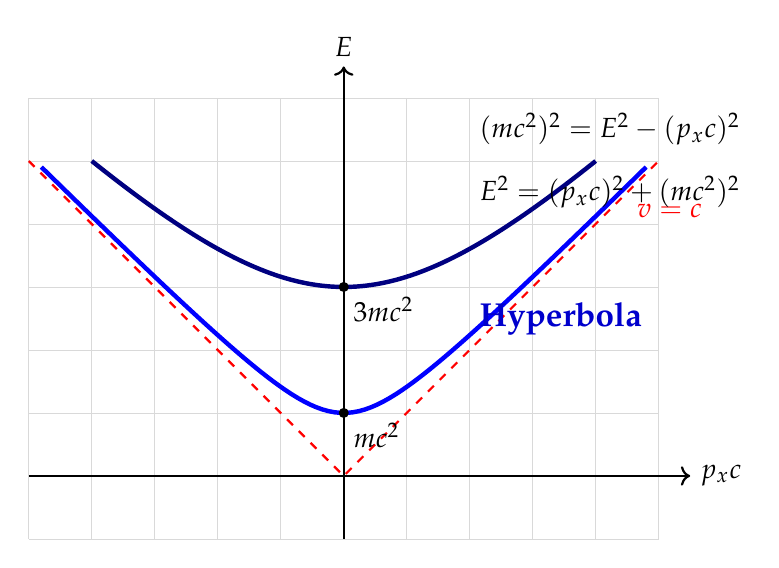
\begin{tikzpicture}[scale=0.8]
    % Grid
    \draw[step=1cm,gray!30,very thin] (-5,-1) grid (5,6);
    
    % Axes
    \draw[thick,->] (-5,0) -- (5.5,0) node[right] {$p_xc$};
    \draw[thick,->] (0,-1) -- (0,6.5) node[above] {$E$};
    
    % Asymptotes E = +/- p_xc
    \draw[dashed, red, thick] (-5,5) -- (0,0) -- (5,5);
    \node[red, right] at (4.5, 4.2) {$v=c$};
    
    % Hyperbola for mass m (intercept mc^2 = 1)
    \draw[ultra thick, blue, domain=-4.8:4.8, samples=100] plot (\x, {sqrt(\x*\x + 1)});
    \node[below right] at (0,1) {$mc^2$};
    \filldraw[black] (0,1) circle (2pt);
    
    % Hyperbola for mass 3m (intercept 3mc^2 = 3)
    \draw[ultra thick, blue!50!black, domain=-4:4, samples=100] plot (\x, {sqrt(\x*\x + 9)});
    \node[below right] at (0,3) {$3mc^2$};
    \filldraw[black] (0,3) circle (2pt);
    
    % Labels
    \node[anchor=west] at (2, 5.5) {$(mc^2)^2 = E^2 - (p_xc)^2$};
    \node[anchor=west] at (2, 4.5) {$E^2 = (p_xc)^2 + (mc^2)^2$};
    \node[anchor=west, text=blue!80!black, font=\large] at (2, 2.5) {\textbf{Hyperbola}};
\end{tikzpicture}
\end{center}
\begin{solution}
(a) Both $p_x c$ and $E$ have units of energy, allowing us to plot them on the same scale. Energy $E = \gamma mc^2$ is strictly positive for a massive particle, but $p_x c$ can be positive or negative.

(d) A hyperbola. The asymptotes are the lines $E = \pm p_x c$, representing the light-like limit where $v \to c$.
\end{solution}

% ==================== LECTURE 9 ====================
\chapter{Composite Systems}

\section{Composite system of particles}

In Newtonian mechanics, the mass of a composite system is simply the sum of the masses of the constituents. This is not accurate in relativity -- as we will now see.

\begin{exercise}[Exercise 1]
Consider a composite system of $N$ particles, each with four-momentum $p^\mu_i = (\frac{E_i}{c}, \vec{p}_i)$, $i = 1, 2, ... N$. Now consider the four-component vector whose components are equal to the \textit{sum} of the individual energies or momentum components -- i.e., the total energy and the total three-momentum:
\[ p^\mu_{\text{tot}} = \sum_i p^\mu_i = \left(\sum_i \frac{E_i}{c}, \sum_i \vec{p}_i\right) = \left(\frac{E_{\text{tot}}}{c}, \vec{p}_{\text{tot}}\right). \]
\begin{enumerate}[label=(\alph*)]
    \item How do these elements ($E_{\text{tot}}/c$ and $\vec{p}_{\text{tot}}$) transform between inertial frames? Briefly justify your response.
    \item What does this allow you to say about the quantity $E_{\text{tot}}^2 - (p_{\text{tot}}c)^2$?
\end{enumerate}
\end{exercise}
\begin{solution}
(a) Since the Lorentz transformations are linear, the sums of the components transform the same way as the individual components. Therefore, $p^\mu_{\text{tot}}$ transforms as a valid four-vector!

(b) Since $p^\mu_{\text{tot}}$ is a four-vector, its invariant square $E_{\text{tot}}^2 - (P_{\text{tot}}c)^2$ must be an invariant quantity in all reference frames. We can set it equal to $(Mc^2)^2$, where $M$ is the invariant mass of the system.
\end{solution}

$\implies$ The \textit{four-momentum} of the system is the sum of the constituent four-momenta. Since $p^\mu_{\text{tot}}$ is a four-vector, $E_{\text{tot}}^2 - (p_{\text{tot}}c)^2$ must be an invariant quantity -- i.e., the same in all inertial frames. We call this invariant quantity the ``invariant mass of the system'' and denoted it with the symbol $m$ (for invariant mass):
\begin{equation}
    (mc^2)^2 \equiv E_{\text{tot}}^2 - (p_{\text{tot}}c)^2
\end{equation}

\begin{exercise}[Question]
$E_{\text{tot}} = \sum E_i$ and $\vec{p}_{\text{tot}} = \sum \vec{p}_i$. Is $m = \sum m_i$? (Or, in words, is the invariant mass of the system necessarily equal to the sum of the masses of the constituents?) Why or why not?
\end{exercise}
\begin{solution}
No. $m = \frac{1}{c^2}\sqrt{(\sum E_i)^2 - (\sum \vec{p}_i c)^2} \neq \sum m_i$. Energy and momentum add linearly, but mass does not!
\end{solution}

\begin{exercise}[Exercise 2]
An example -- Two massless photons each with energy $E$ are about to collide head-on. What is the ``invariant mass of the system of two photons''? (Assume the two photons are traveling toward each other along the $x$ axis.)
\end{exercise}
\begin{solution}
\begin{align*}
    p_{x,1}c &= +E \quad \text{and} \quad p_{x,2}c = -E \\
    p^\mu_{\text{tot}}c &= (E, E, 0, 0) + (E, -E, 0, 0) \tag*{\textcolor{gray}{write down elements for each photon}} \\
    &= (2E, 0, 0, 0) \tag*{\textcolor{gray}{add the 4-momenta component by component}} \\
    (mc^2)^2 &= (2E)^2 - 0 = 4E^2 \tag*{\textcolor{gray}{use equation (1)}} \\
    \implies mc^2 &= 2E
\end{align*}
\end{solution}

$\implies$ A system of massless particles can have non-zero invariant mass!

\begin{exercise}[Question]
Is the invariant mass of an isolated system of particles a \textit{conserved} quantity? Why or why not?
\end{exercise}
\begin{solution}
Yes. If total energy and total momentum are conserved, then $E_{\text{tot}}^2 - (p_{\text{tot}}c)^2$ must also be conserved.
\end{solution}

\begin{exercise}[Exercise 3]
Another example -- Consider a single spring-loaded object that flies apart into two pieces, each of mass $m$ with speed $v > 0$ (like the classical example you considered in Lecture 7). Which of the following expressions is true for the mass $M$ of the object \textit{before} it flies apart?
\begin{enumerate}[label=\roman*.]
    \item $M < 2m$
    \item $M = 2m$ (of course!?)
    \item $M > 2m$
\end{enumerate}
Now check your answer by finding an expression for $M$ by considering the \textit{conserved} and \textit{invariant} mass of the system \textbf{after} the object flies apart.
\textit{Hint: Use the definition of invariant mass in equation (1) and recall that $E_i = \gamma m_i c^2$ for an individual object.}
\end{exercise}
\begin{solution}
iii. $M > 2m$.
To see why, let's look at the system after it flies apart:
\begin{align*}
    (Mc^2)^2 &= (E_{\text{tot}})^2 - (P_{\text{tot}}c)^2 \\
    P_{\text{tot}} &= 0 \quad \text{(since the pieces fly in opposite directions)} \\
    E_1 &= E_2 = \gamma mc^2 \\
    E_{\text{tot}} &= 2\gamma mc^2 \\
    \text{So, } (Mc^2)^2 &= (2\gamma mc^2)^2 \implies M = 2\gamma m.
\end{align*}
Since $\gamma > 1$ for $v > 0$, $M > 2m$.
\end{solution}

\begin{exercise}[Exercise 4]
How large is the effect? For example, what is the fractional increase in mass of the compressed object compared to the sum of the masses of its parts ($2m$), if the parts fly apart at 3 m/s?
Use $c = 3 \times 10^8$ m/s. \textit{(No calculators needed or allowed!)} \\
\textit{Hint: Try a binomial expansion\dots}
\end{exercise}
\begin{solution}
The fractional increase in mass is given by
\begin{align*}
    \frac{M - 2m}{2m} &= \frac{2\gamma m - 2m}{2m} = \gamma - 1 = \left(1 - \frac{v^2}{c^2}\right)^{-1/2} - 1 \\
    &\approx 1 + \frac{1}{2}\frac{v^2}{c^2} - 1 = \frac{1}{2}\frac{v^2}{c^2} \\
    &= \frac{1}{2} \left(\frac{3}{3 \times 10^8}\right)^2 = \frac{1}{2} (10^{-8})^2 = \frac{1}{2} \times 10^{-16}
\end{align*}
\end{solution}

\begin{exercise}[Exercise 5]
Is invariant mass a \textit{relevant} physical quantity? For example, is it the same as the inertial mass that appears in Newton's 2nd Law $\vec{F} = m\vec{a}$, or the gravitational mass that appears in $F_g = mg$?
\end{exercise}
\begin{solution}
Yes.
\end{solution}

\begin{exercise}[Exercise 6]
Consider the following three masses:
\begin{enumerate}[label=(\roman*)]
    \item the mass of a Hydrogen atom in the ground state: $m(\text{H})$;
    \item the mass of a Hydrogen atom in an excited state: $m(\text{H}^*)$;
    \item the mass of an unbound proton + the mass of an unbound electron: $m(p) + m(e)$.
\end{enumerate}
Are the masses all the same? If not, which is lowest? Which is highest? Explain your answer in the context of what you have learned this week.
\end{exercise}
\begin{solution}
No.
\[ m(\text{H}) < m(\text{H}^*) < m(p) + m(e) \]
The ground state Hydrogen atom has the lowest energy (it is tightly bound), so its invariant mass is the lowest. The excited state has more energy, so it is slightly more massive. The fully unbound proton and electron have the highest total energy, hence the highest mass.
\end{solution}

\section{The electron-Volt -- a unit of energy.}

When dealing with mass, energy, and momentum of atoms, nuclei and elementary particles, mks units like Joules are very impractical -- they are just too large. A more convenient unit is the `electron-Volt' (abbreviated as eV), which is defined as the amount of (kinetic) energy that an electron aquires when it is accelerated from rest through an electric potential difference of one Volt. It is a very small unit of energy compared to the Joule: 1 electron-Volt $= 1.6 \times 10^{-19}$ Joules.

\begin{exercise}[Quick Exercise]
Show that the above conversion factor from electron-Volts (eV) to Joules (J) is correct by using the fact that the charge of an electron is $1.6 \times 10^{-19}$ C and anything you can remember about the relationship between a Coulomb, a Volt, and a Joule in the mks system.
\end{exercise}
\begin{solution}
\begin{align*}
    q_e &= 1.6 \times 10^{-19} \text{ C} \\
    V &= \frac{\text{J}}{\text{C}} \\
    W &= q \Delta V \\
    1 \text{ eV} &= (1.6 \times 10^{-19} \text{ C})(1 \text{ V}) = 1.6 \times 10^{-19} \text{ J}
\end{align*}
\end{solution}

Atomic binding energies are typically in the range of a few eV to keV (\textbf{thousands} of electron-Volts).

Binding energies in nuclear physics are on the order of MeV (\textbf{millions} of electron-Volts).

And particle accelerators can create particles with rest energies ($mc^2$) on the order of GeV (\textbf{billions} of electron volts) to hundreds of GeV.

\begin{exercise}[Exercise 7]
Quantifying the difference\dots What is the approximate fractional difference between the sum of the masses of a proton and an electron, and the mass of a Hydrogen atom in the ground state?
(It will be helpful to know that the rest mass energy of a Hydrogen atom is very close to 1 GeV. Do you know the binding energy of Hydrogen, in eV?)
\end{exercise}
\begin{solution}
The binding energy of Hydrogen is 13.6 eV. Therefore the difference in mass energy is 13.6 eV.
The fractional difference is $\frac{13.6 \text{ eV}}{1 \text{ GeV}} = \frac{13.6}{10^9} \approx 1.36 \times 10^{-8}$.
\end{solution}

% ==================== LECTURE 10 ====================
\chapter{Recap and an Example: Two-body Decay}

\textbf{Conserved and invariant quantities.} Consider each quantity given below for an \textit{isolated system} of possibly \textit{interacting} particles with masses $m_i > 0$ and velocities $\vec{v}_i \equiv \Delta \vec{x}_i / \Delta t = (v_{x,i}, 0, 0)$ as measured in an inertial frame. The factor $\gamma_i$ is defined by
\[ \gamma_i \equiv \left(1 - \frac{v_i^2}{c^2}\right)^{-\frac{1}{2}}. \]

Work with your group on the following exercises:
\begin{enumerate}[label=(\alph*)]
    \item Identify the precise and accurate \textit{name} or \textit{description} for each of the five quantities.
    \item Then indicate with a \textbf{Y} for ``yes'' or an \textbf{N} for ``no'' whether the quantity is conserved in time, and whether it is invariant (the same in all inertial frames), \textit{in special relativity}.
    \textit{Tip:} If applicable, write the quantity in each summation in a different form.
\end{enumerate}

\begin{exercise}[Quantity 1]
$\sum_i m_i c^2$
\end{exercise}
\begin{solution}
Conserved? \textbf{N} \quad Invariant? \textbf{Y} \\
Name or brief description: Sum of rest energies.
\end{solution}

\begin{exercise}[Quantity 2]
$\sum_i \gamma_i m_i c^2$
\end{exercise}
\begin{solution}
Conserved? \textbf{Y} \quad Invariant? \textbf{N} \\
Name or brief description: Total energy of the system ($E_{\text{tot}}$).
\end{solution}

\begin{exercise}[Quantity 3]
$\sum_i m_i v_{x,i}$
\end{exercise}
\begin{solution}
Conserved? \textbf{N} \quad Invariant? \textbf{N} \\
Name or brief description: Sum of Newtonian momenta.
\end{solution}

\begin{exercise}[Quantity 4]
$\sum_i \gamma_i m_i v_{x,i}$
\end{exercise}
\begin{solution}
Conserved? \textbf{Y} \quad Invariant? \textbf{N} \\
Name or brief description: Total relativistic momentum ($p_{x, \text{tot}}$).
\end{solution}

\begin{exercise}[Quantity 5]
$\left(\sum_i \gamma_i m_i c^2\right)^2 - \left(\sum_i \gamma_i m_i v_{x,i} c\right)^2$
\end{exercise}
\begin{solution}
Conserved? \textbf{Y} \quad Invariant? \textbf{Y} \\
Name or brief description: Invariant mass of the system $(Mc^2)^2$.
\end{solution}

\section{An example -- ``Two-body Decay'' (\textit{thinking} through a problem)}

Consider particle A, \textit{at rest}, decaying into particles B and C: A $\to$ B + C. Denote their masses by $m_A$, $m_B$, and $m_C$.

In this problem, you will learn how to find expressions for the energy and momentum of the outgoing particles: $E_B, E_C, p_B,$ and $p_C$. (Remember that $p_i \equiv |\vec{p}_i|$.) But first, we will use physical reasoning to make a few predictions.

\begin{enumerate}[label=(\alph*)]
    \item Draw a picture of the situation before and after particle A decays. Add labels corresponding to any information you are given in the problem.
    \item Write the four-momentum $p^\mu_i$ for each particle. (Write the components only in terms of what you are given or what you are trying to find. If you \textit{know} any components are 0, go ahead and use that information.)
    \item On which quantities could the energy and momentum of the outgoing particles possibly depend?
    \item Write expressions for conservation of total energy and conservation of total momentum for this decay process, in terms of only quantities you are given ($m_A, m_B, m_C$) or quantities you want to find ($E_B, E_C, p_B, p_C$).
    
    Conservation of total energy: $m_A c^2 = E_B + E_C$
    
    Conservation of total momentum: $0 = \vec{p}_B + \vec{p}_C$ (or $p_B = p_C$)
    \item Identify two specific special cases of $m_B$ and $m_C$ for which you can predict $E_B, E_C, p_Bc$ and $p_Cc$ in terms of \textbf{only} $m_Ac^2$.
    
    Case I:
    
    Case II:
    \item Now identify two conditions on $m_B$ and $m_C$ that are more general than those we found in (e), for which you can predict $E_B, E_C, p_Bc$ and $p_Cc$ in terms of only the \textbf{given quantities} $m_A, m_B$ and $m_C$ -- but \textit{not} in terms of \textbf{only} $m_A$?
    
    Case A:
    
    Case B:
\end{enumerate}

\begin{enumerate}[label=(\alph*)]
\setcounter{enumi}{6}
    \item Now follow the hints below to find the energy of particle B (in terms of only quantities you are given) for the general case. If you get bogged down in algebra, go directly to the result, check that the dimensions make sense, and then move on to the next part. (You will complete the details of this part on Problem Set 4.)
    
    First note that conservation of total energy and total momentum provides two constraints. However, we have (for general masses $m_A, m_B$, and $m_C$) four unknowns: $E_B, E_C, p_B,$ and $p_C$. Therefore, we need to bring in more constraints. How? Through expressions for the single-particle invariant masses!
    
    First copy the expressions for conservation of total energy and total momentum from part (d) above:
    \vspace{2cm}
    
    Next write an expression for the invariant mass of C in terms of its energy and momentum:
    \[ (m_Cc^2)^2 = E_C^2 - (p_Cc)^2 \]
    
    Now start with this expression for $(m_Cc^2)^2$ and use the expressions for conservation of total energy and total momentum to eventually find $E_B$. (Follow the guidance in the annotations on the right below.)
    \begin{align*}
        (m_Cc^2)^2 &= \qquad\qquad\qquad\qquad\qquad \text{\small Use cons'n of energy: } E_C = m_Ac^2 - E_B. \\
                   &= \qquad\qquad\qquad\qquad\qquad \text{\small Use } E_B^2 = (m_Bc^2)^2 + (p_Bc)^2. \\
                   &= \\
                   &=
    \end{align*}
    
    Now solve for $E_B$ to get the final result in terms of only $m_A, m_B$, and $m_C$:
    \begin{equation}
        E_B = \frac{m_A^2 + m_B^2 - m_C^2}{2m_A} c^2.
    \end{equation}
    
    Check that this result is dimensionally consistent with energy.
    
    Without doing any further calculation, write down an expression for $E_C$:
    \begin{equation}
        E_C = \frac{m_A^2 + m_C^2 - m_B^2}{2m_A} c^2.
    \end{equation}
    
    \item Check that your solutions for $E_B$ and $E_C$ give the expected results for the four cases you identified in parts (e) and (f) above.
    
    Case I: \vspace{1cm}
    
    Case II: \vspace{1cm}
    
    Case A: \vspace{1cm}
    
    Case B: \vspace{1cm}
\end{enumerate}

\begin{enumerate}[label=(\alph*)]
\setcounter{enumi}{8}
    \item Which equation (or equations) would we now use to find the magnitude of the momentum of each of the outgoing particles ($p_B$ and $p_C$) in terms of quantities that we are given?
    \vspace{2cm}
    \item We will not ask you to do the algebra, but here is what you would find for the momenta (times $c$) of particles B and C:
    \[ p_Bc = p_Cc = \frac{c^2}{2m_A} \left[ m_A^4 + m_B^4 + m_C^4 - 2m_A^2m_B^2 - 2m_A^2m_C^2 - 2m_B^2m_C^2 \right]^{1/2}. \]
    It turns out that the quantity under the radical can be factored:
    \begin{align*}
        p_Bc &= p_Cc \\
             &= \frac{c^2}{2m_A} \Big[ (m_A + m_B + m_C)(m_A + m_B - m_C)(m_A - m_B + m_C)(m_A - m_B - m_C) \Big]^{1/2}.
    \end{align*}
    Check that the above expressions for $p_Bc = p_Cc$ are dimensionally consistent with your expectations for momentum (times $c$).
    \vspace{2cm}
    
    Check that the above expressions for $p_Bc = p_Cc$ give the expected results for the four cases you identified in parts (e) and (f) above.
    
    Case I: \vspace{1cm}
    
    Case II: \vspace{1cm}
    
    Case A: \vspace{1cm}
    
    Case B: \vspace{1cm}
\end{enumerate}

% ==================== LECTURE 11 ====================
\chapter{Dimensional Analysis}

In today's lesson, we will see how it is possible to deduce a great deal about the equations that describe the behavior of a complex physical system through an analysis of \textbf{dimensions} -- with some physical reasoning thrown in.

\textbf{First, a note about units\footnote{We will not discuss different systems of units and significant figures in class, but please do read Sec. 6.6.2 in Morin's text on Special Relativity and Note 1.5 (p. 40) Sections 2.7 and 2.8 (pp. 59-64) in Kleppner \& Kolenkow, which include an interesting history of how the commonly used units are defined.}:} As of 2019, all units relevant in mechanics are defined in terms of quantum mechanical phenomena or in terms of fundamental constants of nature.
\begin{itemize}
    \item The standard of \textbf{time} is defined in terms of the frequency of light emitted by a specific atom when it changes from one state to another.
    \begin{itemize}
        \item As of 1967, 1 second is defined as the duration of exactly 9,192,631,770 vibrations of an electromagnetic wave emitted by a specific isotope of the cesium atom when it undergoes a particular atomic transition.
    \end{itemize}
    \item The standard of \textbf{length} is defined in terms of the speed of light in vacuum, combined with the time standard.
    \begin{itemize}
        \item As of 1983 (reworded in 2019), 1 meter is defined as the length of the path traveled by light in vacuum during a time interval of 1/299,792,458 of a second.
    \end{itemize}
\end{itemize}

\begin{exercise}[Quick Exercise 1]
What is the exact value of $c$ when expressed in SI units? \\
What is the exact value of a light-second in SI units?
\end{exercise}
\begin{solution}
The exact value of $c$ is $299,792,458$ m/s. \\
The exact value of a light-second is $299,792,458$ m $\simeq 3.0 \times 10^8$ m.
\end{solution}

The important point is not the specific values given here, but that these ``everyday'' units (meters and seconds) are defined in terms of fundamental physics!

What about units of mass? How is the kilogram defined?
\begin{itemize}
    \item Until 2019, the kilogram was defined by a 143-year-old platinum alloy cylinder housed in the International Bureau of Weights and Measures in Paris.
    \item The kilogram is \textit{now} defined in terms of Planck's constant ($h$), which has been measured with extraordinary (reproducible) precision in recent years in quantum systems.\footnote{See, for example, this National Institute for Standards and Technology (NIST) website: \url{https://www.nist.gov/si-redefinition/kilogram-mass-and-plancks-constant}}\textsuperscript{,}\footnote{To learn how this definition of the kilogram can be used in practice, see this wonderful lecture by Professor Wolfgang Ketterle from MIT, which was delivered as part of a Stanford Physics Department public lecture series in 2020: \url{https://www.youtube.com/watch?v=lSN7gslzjgY} (If you want to skip the introduction, start at 8:50 minutes.)}
    \item The value of Planck's constant has now been set as exactly $6.626\,070\,15 \times 10^{-34} \text{ kg\,m}^2\text{s}^{-1}$.
    \item When combined with the definition of the meter and the second, the value of Planck's constant now defines the kilogram.
\end{itemize}

We will consistently use SI units in this class with one exception. As described earlier, when dealing with relativistic energy or momentum (times $c$) or rest mass (times $c^2$), it is often more convenient to deal with a unit of energy called the electron-volt, defined as the amount of kinetic energy gained by an electron when it is accelerated through a potential difference of 1 Volt (in vacuum). As you showed in Lecture 9, an electron-volt (eV) is a very small unit of energy compared to the Joule: 1 electron-Volt $= 1.6 \times 10^{-19}$ Joules.

\section{Dimensions and Units -- They are not the same!}

First, let's start with dimensions. Most quantities that we deal with in physics (such as period of oscillation, $T$, or length of a string, $\ell$) have ``dimensions'' associated with them.
\begin{itemize}
    \item In mechanics we can almost always get away with just three fundamental dimensions: \textbf{mass, length and time}.
    \item We will use bold-face, upper-case letters to denote these dimensions: \textbf{M}, \textbf{L} and \textbf{T}.
    \item Non-boldface, lower-case letters will denote the names of variables that have these dimensions; for example, mass $m$, distance $d$, or time $t$.
\end{itemize}

In the table below, we summarize the basic dimensions used in mechanics, the variables that have these dimensions, and sample units.

\begin{center}
\begin{tabular}{ccc}
Dimension & Variable & Sample Units \\
\hline
\textbf{M} & mass $m$ & kg, g, pound-mass \\
\textbf{L} & distance $d$ & m, cm, feet \\
\textbf{T} & time $t$ & s, weeks, years \\
\hline
\end{tabular}
\end{center}

The notion of a variable's dimensions should be distinguished from the variable itself. For example, consider the variable mass and the dimensions of mass.
\begin{itemize}
    \item The variable $m$, representing the mass of an object, can eventually be replaced by a number, the value of which will depend on the chosen units, such as kg or grams.
    \item The dimension \textbf{M} identifies the physical character of the variable $m$, but has nothing to do with its magnitude.
\end{itemize}

We will use square brackets [ ] around a variable to denote the dimensions of that variable:
\[ [m] = \textbf{M}, \quad [d] = \textbf{L}, \quad [t] = \textbf{T}. \]

\begin{itemize}
    \item Units are also distinct from dimensions -- we only need to choose units for a variable in an equation \textit{if or when we assign a numerical value to the variable.}
    \item The numerical value of each variable depends on the size of the chosen unit.
\end{itemize}

\begin{tcolorbox}[colback=white, colframe=black, boxrule=0.5pt, arc=0pt]
Summary:
\begin{enumerate}
    \item Variables have \textit{dimensions} (not units).
    \item Only numerical values have associated \textit{units}.
\end{enumerate}
\end{tcolorbox}

Example -- Acceleration has dimensions that include both length and time: $a = \frac{d^2x}{dt^2}$.

\begin{exercise}[Quick Exercise 2]
Write the dimensions of acceleration:
\end{exercise}
\begin{solution}
\[ [a] = \textbf{L}^1\textbf{T}^{-2} \]
\end{solution}

Let's now consider the relation corresponding to Newton's Second Law, $F_x = ma_x$.
\begin{itemize}
    \item This equation expresses the fact that a force $F$ applied to an object will result in an acceleration $a$, and the amount of force needed to produce a particular acceleration is proportional to the inertial mass $m$ of the object.
    \item $F, m$ and $a$ are physical variables.
    \item Each variable has well-defined dimensions.
\end{itemize}

An equation must always be dimensionally correct -- i.e., the dimensions of the quantities on the left and the right of the equal sign must be the same.

\begin{exercise}[Quick Exercise 3]
Write the dimensions of force using $F = ma$:
\end{exercise}
\begin{solution}
\[ [F] = \textbf{M}[a] = \textbf{M}\textbf{L}\textbf{T}^{-2} \]
\end{solution}

Only if the dimensions of $F$ match those of $ma$ will the relation $F = ma$ remain true, independent of the size of the units used to measure each quantity.
\begin{itemize}
    \item For example, the numerical value of the variable $m$ will be larger if the units used for $m$ are grams rather than kilograms.
    \item $\implies$ Dimensions of mass \textit{must} appear to the same power (i.e., with the \textit{same exponent}) on both sides of the equation -- else the validity of the equation will depend on the units one chooses!
\end{itemize}

\section{Dimensional Analysis}

In the next exercise, you'll work with a simple example (period of a pendulum) that illustrates the basic methods of dimensional analysis before moving on to a more complex example (radius of a black hole). Here are the steps:
\begin{enumerate}[label=(\alph*)]
    \item Identify the physical variables and any dimensionful\footnote{By ``dimensionful'', we mean a constant that has dimensions. This is in contrast to dimensionless constants such as $\pi$, 1/2, etc.} fundamental constants on which the answer \textit{could} depend.
    \item Write down the dimensions of these quantities.
    \item Demand that these quantities be combined in a functional relation such that the equation is dimensionally consistent.
\end{enumerate}

\section{An application of dimensional analysis: Period of a Pendulum}

We will use dimensional analysis (and one simple experiment) to determine the equation for the period of oscillation for a pendulum near the surface of the earth. That is, how much time does it take a bob of mass $m$, at the end of a string (of negligible mass) of length $\ell$, to swing back and forth through one complete oscillation? (See the figure below.)

Assume for a few minutes that you have \textit{never} seen or derived the equation for the period of oscillation for a simple pendulum--or, if you have, that you have forgotten it!

\begin{center}
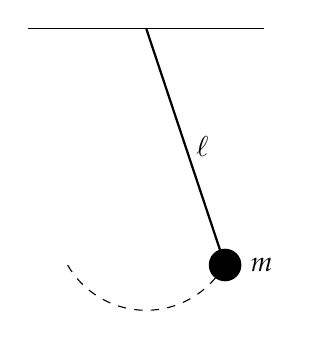
\begin{tikzpicture}
    % Ceiling
    \draw (-1.5,0) -- (1.5,0);
    
    % Pendulum
    \draw[thick] (0,0) -- (1,-3) node[midway, right] {$\ell$};
    \filldraw[black] (1,-3) circle (0.2) node[right=2mm] {$m$};
    
    % Swing path
    \draw[dashed, ->] (-1,-3) arc (210:330:1.15);
\end{tikzpicture}
\end{center}

\begin{exercise}[Exercise 4]
\begin{enumerate}[label=(\alph*)]
    \item For the first step, we must always use physical reasoning. On which physical variables \textit{might} the period\footnote{Note that we use a boldface \textbf{T} to denote dimensions of time, and a non-boldface, slanted $T$ to denote the period of the pendulum.} $T$ of oscillation of the pendulum depend? Identify all variables describing the bob, the string, and the relevant force.
    \item Now assume that the period $T$ can be expressed as a product of these variables each raised to an unknown power. To more easily distinguish variables and exponents, use the Greek letters $\alpha, \beta, \gamma, \dots$ for the exponents.\footnote{$\alpha$ is the Greek letter \textit{alpha}, $\beta$ is the Greek letter \textit{beta}, and $\gamma$ is the Greek letter \textit{gamma}.} Include in your product a dimensionless constant $k$ to allow for numbers like $2, 4, \pi, \dots$
    \item Now find the values of $\alpha, \beta, \gamma, \dots$ that make the dimensions of the right-hand side the same as the dimensions of the left-hand side.
    \item Given your result, estimate the factor by which the period changes if the length of the string is shortened by a factor of 4. How about if the mass is doubled? By how much would the period change if the pendulum were taken to the moon? ($g_{\text{moon}} \approx g_{\text{earth}}/6$)?
    \item In class, we have a pendulum with length $\ell = 1$ m and many of you have a timer -- e.g., on your phone. How can we determine the dimensionless constant $k$? (You can assume we know that the value of $g$ is $9.8\text{ m/s}^2$, which is ample precision for our current purpose.)
\end{enumerate}
\end{exercise}
\begin{solution}
(a) Period could depend on mass $m$, length $\ell$, and the acceleration due to gravity $g$.

(b) $T = k \ell^\alpha m^\beta g^\gamma$

(c) Dimensions: $[T] = \textbf{T}$, $[\ell] = \textbf{L}$, $[m] = \textbf{M}$, $[g] = \textbf{L}\textbf{T}^{-2}$.
\[ \textbf{T}^1 = \textbf{L}^\alpha \textbf{M}^\beta (\textbf{L}\textbf{T}^{-2})^\gamma = \textbf{L}^{\alpha+\gamma} \textbf{M}^\beta \textbf{T}^{-2\gamma} \]
Equating exponents:
\begin{align*}
    \text{\textbf{M}: } \beta &= 0 \implies \text{No mass dependence!} \\
    \text{\textbf{T}: } 1 &= -2\gamma \implies \gamma = -1/2 \\
    \text{\textbf{L}: } 0 &= \alpha + \gamma \implies \alpha = 1/2
\end{align*}
So $T = k \ell^{1/2} g^{-1/2} = k\sqrt{\frac{\ell}{g}}$.

(d) If length is shortened by a factor of 4, the period decreases by a factor of 2. If mass is doubled, the period is unchanged! If taken to the moon, the period increases by a factor of $\sqrt{6}$.

(e) We can just measure the period! For $\ell = 1$ m, we get $t \approx 2$ sec.
\[ t = k\sqrt{\frac{1 \text{ m}}{9.8 \text{ m/s}^2}} \implies k = \frac{t}{\sqrt{\frac{1}{9.8}}} \approx \frac{2}{1/\pi} = 2\pi. \]
\end{solution}

\section{Black holes in the news!}

\begin{itemize}
    \item The 2017 Nobel Prize in Physics was awarded to the leadership of the Laser Interferometer Gravitational-Wave Observatory (LIGO) collaboration of over one thousand researchers from more than twenty countries for the detection of gravitational waves from the mergers of ``stellar mass'' pairs of black holes.
    \begin{itemize}
        \item LIGO uses the detected gravitational waves to measure the masses of the initial black holes and the final black hole in a merger.
    \end{itemize}
    \item The 2020 Nobel Prize in Physics was awarded to Roger Penrose ``for the discovery that black hole formation is a robust prediction of the general theory of relativity'', and Reinhard Genzel and Andrea Ghez ``for the discovery of a super-massive compact object at the centre of our galaxy'' -- called Sagittarius A*.
    \begin{itemize}
        \item Genzel and Ghez use the orbits of stars circulating Sagittarius A* to measure its mass.
    \end{itemize}
    \item In May 2022, the Event Horizon Telescope (EHT) Collaboration provided the first ``images'' of Sagittarius A*, based on observations from a worldwide network of radio telescopes. This breakthrough followed the EHT collaboration's 2019 release of the first image of a much larger black hole, called M87*, at the centre of the more distant Messier 87 galaxy.
    \begin{itemize}
        \item EHT measures the size of a black hole by imaging gas moving at near relativistic speeds in the vicinity of the black hole.
    \end{itemize}
\end{itemize}

Black hole masses range from ``stellar-mass'' black holes for LIGO ($m_{\text{stellar}} \approx 10M_{\text{sun}}$, where $M_{\text{sun}}$ is called a ``solar mass'') to super-massive black holes ($m_{\text{super}} \approx 10^7M_{\text{sun}}$ for the black hole near the center of our galaxy).
\begin{itemize}
    \item What is the corresponding range of \textbf{radii} of black holes? How about \textbf{density}?
\end{itemize}

You will now answer these questions using \textit{only} dimensional analysis!

\begin{exercise}[Exercise 5]
In this exercise, you will derive the relationship between the two parameters that essentially define a black hole: its mass $m$ and its radius $R$.
\begin{enumerate}[label=(\alph*)]
    \item On which physical variables or fundamental constants might the radius $R$ depend? Write down the dimensions of each.
    \item Find the expression for $R$, up to a dimensionless constant $k$. Use the ``formal'' method of dimensional analysis described earlier in this lecture.
    \item In responding to the following questions, \textbf{do not} plug in the values of any fundamental constants of nature! Instead, work only with dimensionless ratios.
    \begin{enumerate}[label=(\roman*)]
        \item What is the ratio of the radius of the super-massive black hole at the center of our galaxy ($m_{\text{super}} \approx 10^7 M_{\text{sun}}$) to the radius of a 10 solar-mass black hole? Which has the larger radius?
        \item What is the ratio of the average mass density of matter in the super-massive black hole at the center of our galaxy to the average mass density in the 10 solar-mass black hole? Which has the higher density?
    \end{enumerate}
\end{enumerate}
\end{exercise}
\begin{solution}
(a) The radius of a black hole depends on its mass $m$, the gravitational constant $G$, and the speed of light $c$.
Dimensions: $[m] = \textbf{M}$, $[G] = \textbf{L}^3\textbf{M}^{-1}\textbf{T}^{-2}$, $[c] = \textbf{L}\textbf{T}^{-1}$.

(b) We want to form a length $R$ from $m, G, c$: $R = k m^\alpha G^\beta c^\gamma$.
\[ \textbf{L} = \textbf{M}^\alpha (\textbf{L}^3\textbf{M}^{-1}\textbf{T}^{-2})^\beta (\textbf{L}\textbf{T}^{-1})^\gamma = \textbf{L}^{3\beta+\gamma} \textbf{M}^{\alpha-\beta} \textbf{T}^{-2\beta-\gamma} \]
Equating exponents:
\begin{align*}
    \text{\textbf{M}: } 0 &= \alpha - \beta \implies \alpha = \beta \\
    \text{\textbf{T}: } 0 &= -2\beta - \gamma \implies \gamma = -2\beta \\
    \text{\textbf{L}: } 1 &= 3\beta + \gamma = 3\beta - 2\beta = \beta \implies \beta = 1
\end{align*}
So $\alpha = 1, \beta = 1, \gamma = -2$. The expression is $R = k\frac{Gm}{c^2}$.

(c) (i) Since $R \propto m$, the ratio of the radii is simply the ratio of the masses:
\[ \frac{R_{\text{super}}}{R_{\text{stellar}}} = \frac{10^7 M_{\text{sun}}}{10 M_{\text{sun}}} = 10^6. \]

(c) (ii) Density $\rho = \frac{m}{\frac{4}{3}\pi R^3} \propto \frac{m}{R^3}$. Since $R \propto m$, we have $\rho \propto \frac{m}{m^3} = \frac{1}{m^2}$.
\[ \frac{\rho_{\text{super}}}{\rho_{\text{stellar}}} = \left(\frac{m_{\text{stellar}}}{m_{\text{super}}}\right)^2 = (10^{-6})^2 = 10^{-12}. \]
The stellar mass black hole is vastly more dense!
\end{solution}

\textcolor{blue}{\textit{Note: A black hole does not actually have uniform density, but the average density is roughly how dense a given amount of mass $m$ must be before it forms a black hole.}}

\section{Dimensions and Mathematical Formulae}

\begin{itemize}
    \item The fact that each term in a physical equation must have the same dimensions can sometimes be used to determine fundamental equations up to a dimensionless constant and can always be used to check whether an equation is blatantly incorrect.
    \item Note that in mathematics classes, dimensions are rarely, if ever, mentioned because the variables are usually not defined as physical quantities.
    \item In particular, in mathematics, you will see mathematical terms like $\sin x$, $\cos y$, and $\exp t$.
\end{itemize}

\begin{exercise}[Exercise 6]
In physics, the quantities $x, y$, and $t$ typically denote quantities that have dimensions (e.g., length \textbf{L} for $x$ and $y$; time \textbf{T} for $t$). In that case, expressions like $\sin x$, $\cos y$, and $\exp t$ are \textit{not} valid because the arguments of the sine, cosine, and exponential functions must be dimensionless. Why must the arguments be dimensionless? (Hint: Consider a Taylor series expansion\dots)
\end{exercise}
\begin{solution}
The Maclaurin/Taylor series expansion involves summing different powers of the argument (e.g., $\sin x = x - \frac{x^3}{3!} + \frac{x^5}{5!} - \dots$). If $x$ had dimensions (e.g., length), we would be adding length to volume to hyper-volume, which is physically meaningless! The dimensions would be infinite/undefined.
\end{solution}

\begin{exercise}[Quick Exercise 7]
Identify physical quantities that could be included in the arguments of the following functions so that the arguments are dimensionless, assuming $t$ is time and $x$ is position.
\[ \cos( \qquad t), \quad \sin( \qquad x ), \quad \exp(-t / \qquad ). \]
\end{exercise}
\begin{solution}
\begin{align*}
    &\cos(2\pi f t) \quad \text{or} \quad \cos(\omega t) \\
    &\sin\left(\frac{2\pi x}{\lambda}\right) \quad \text{or} \quad \sin(kx) \\
    &\exp\left(-\frac{t}{\tau}\right)
\end{align*}
\end{solution}

Also note that the series expansions for the trigonometric functions will only be valid if the argument $\alpha$ is expressed in radians (which is dimensionless), not degrees.

% ==================== LECTURE 12 ====================
\chapter{Special Relativity $\to$ Newtonian Mechanics}

\textbf{Readings:} Newton's Laws -- Secs. 2.1-2.6 in textbook by Kleppner \& Kolenkow; first part of Sec. 6.5 (overview of ``Nonrelativistic dynamics'') in Morin's textbook on Special Relativity.

We're now moving on to a ``limiting case'' of special relativity:
\[ v \ll c \implies \text{classical (Newtonian) mechanics.} \]
This \textit{might} seem like a step backwards from special relativity, so it's important to discuss \textit{why} we're about to spend the rest of the quarter on classical mechanics.

\section{Motivation}

Why go `back' to classical (non-relativistic) mechanics?
\begin{itemize}
    \item \textbf{Practicality:} Other than light, everything we experience on a day-to-day basis is moving non-relativistically, so classical mechanics works really well for many situations!
    \item \textbf{Simplicity:} Everyday interactions (gravity, friction, contact forces) are MUCH easier to model and compute with classical mechanics---we didn't even TRY in special relativity!
    \item \textbf{Wider applicability:} With the simplification of $v \ll c$, we can study objects that do not exist relativistically, without the complication of handling them `realistically'---e.g., taking into account causality, etc. (See, for example, the brief discussion of the non-existence of rigid bodies in special relativity, in qualitative Question 7 on p.\,226 in Morin.)
    \item \textbf{Analogy:} Modern physics is often built up by comparing and contrasting with classical mechanics, so it's an important foundation to build on as you continue studying physics.
    
    \textbf{Example 1} -- Quantum systems, while exhibiting behavior that is bizarre and impossible in classical mechanics, still satisfy equations that are very much analogous to their classical equations of motion -- e.g., those related to angular momentum or potential energy functions. Therefore, a \textit{deep} understanding of classical mechanics is an important tool in interpreting the quantum behavior of a system. In fact, we'll spend time developing a full vector description of rotational motion and a deep understanding of potentials and ``effective potentials'', so that you can fully appreciate the analagous concepts if you go on to study quantum mechanics.
    
    \textbf{Example 2} -- Mathematical analogies can bring physical insight and physical analogies can bring mathematical insights. Sometimes an equation derived in a totally abstract context `looks like' an equation from classical mechanics---and that allows you to use physical reasoning to help guide your problem solving.\footnote{See p. 4 in the essay by Ed Witten uploaded to the module for Lesson 12 in Canvas. Witten is the first (and only, to date) physicist to win the Fields medal, which is the ``Nobel Prize'' of mathematics.}
    
    \textbf{Example 3} -- Euler's disk\footnote{Euler's disk: \url{https://www.youtube.com/watch?v=ug2bKCG4gZY}} and merging black holes as observed by LIGO\footnote{LIGO ``chirp'': \url{https://www.youtube.com/watch?v=AG19o2PmnNo}}.
\end{itemize}

\section{Special Relativity $\to$ Newtonian Mechanics}

Beginning with Einstein's two postulates of Special Relativity, we derived the Lorentz transformations for space and time, for two observers in inertial frames moving relative to each other.
\begin{align*}
    \Delta t' &= \gamma \left( \Delta t - \beta \frac{\Delta x}{c} \right) \\
    \Delta x' &= \gamma ( \Delta x - \beta c \Delta t )
\end{align*}

Recall Einstein's postulates:
\begin{enumerate}
    \item The laws of physics are the same in any inertial frame of reference.
    \item All inertial observers measure the same speed of light in empty space (vaccum).
\end{enumerate}

Einstein's first postulate still holds and is relevant in Newtonian mechanics.

\begin{exercise}[Quick Exercise 1]
Which quantity do we implicitly assume is the same in all inertial frames (i.e., invariant) when transforming between inertial frames in \textit{non-relativistic} physics?
\end{exercise}
\begin{solution}
$t$
\end{solution}

\begin{exercise}[Exercise 2]
Write down the \textit{non-relativistic} transformation equations that relate $\Delta x$ and $\Delta t$ in one inertial frame to $\Delta x'$ and $\Delta t'$ in an inertial frame moving at velocity $u_x$ with respect to the unprimed frame. (Make a sketch!)
\end{exercise}
\begin{solution}
We've already discussed the time interval:
\[ \Delta t' = \Delta t \]
To find $\Delta x'$ in terms of $\Delta x$, you could make a sketch at two different times. Or you could write an expression for $v'_x$ in terms of $v_x$ and $u_x$, and then take it from there\dots
\[ \Delta x' = \Delta x - u_x \Delta t \]
\end{solution}

This non-relativistic transformation is called a ``Galilean'' transformation.

\begin{exercise}[Exercise 3]
Now expand the relativistic Lorentz transformation for a boost $\beta_x = u_x/c$, to \textit{leading order} in $\beta_x$, to find expressions that are valid if $\beta \ll 1$.
\end{exercise}
\begin{solution}
\begin{align*}
    \Delta t' &= \gamma(\Delta t - \beta_x \Delta x/c) \approx \Delta t (1 - \beta^2)^{-1/2} - \beta_x \Delta x / c \\
    \Delta x' &= \gamma(\Delta x - \beta_x c \Delta t) \approx \Delta x - u_x \Delta t
\end{align*}
\end{solution}

Are there any terms with $c$ left in either expression? \\
What \textit{additional} assumptions must one make to eliminate all instances of $c$ -- i.e., to arrive at the Galilean transformation equations? Describe the assumptions as equations or in words.

\begin{exercise}[Exercise 4]
Given the above Galilean transformation, how do velocity and acceleration transform?
\end{exercise}
\begin{solution}
\begin{align*}
    v'_x &\equiv \frac{\Delta x'}{\Delta t'} = \frac{\Delta x}{\Delta t} - u_x = v_x - u_x \\
    a'_x &\equiv a_x
\end{align*}
\end{solution}

This invariance of acceleration but not velocity is what we concluded for Newtonian mechanics in an exercise back in Lesson 1!

\section{Newton's Laws}

Newton's Laws are the postulates of classical mechanics!

You've probably encountered Newton's Laws before in many different `translations.' Here our goal will be to translate them into a form that is both precise and applicable to solving problems---just as we had in the postulates of relativity!

\begin{exercise}[Exercise 5]
Work with your group to write (on your white board) Newton's Laws in any form that you remember them. Be \textit{precise} and try to avoid redundancy between laws.
\end{exercise}
\begin{solution}
\begin{itemize}
    \item $m\vec{a} = \sum_i \vec{F}_i^{\text{ext}}$
    \item Equal and opposite reaction: $\vec{F}_{12} = -\vec{F}_{21}$
    \item Object at rest stays at rest in a given inertial frame.
\end{itemize}
\end{solution}

\begin{exercise}[Exercise 6]
Argue for or against the following statement: ``Newton's 1st Law is redundant because it's implied by Newton's 2nd Law when $\vec{F} = 0$.''
\end{exercise}

\subsection{Untangling Newton's 3rd Law Pairs}

\begin{exercise}[Exercise 7]
On your white board, make a sketch of a block of mass $M$, sitting at rest on a table. Identify all the forces involved in this scenario and identify which forces form ``Newton's 3rd Law pairs''.

When you \textit{think} you are finished, convince yourself that you are correct by checking that each 3rd-Law pair involves the \textit{same type} of force acting on \textit{different} bodies.
\end{exercise}

\begin{exercise}[Exercise 8]
\begin{center}
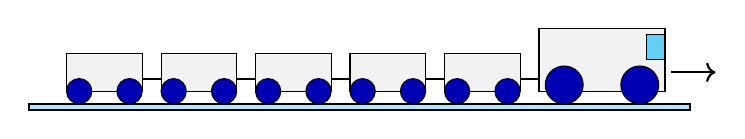
\begin{tikzpicture}[scale=0.8]
    % Ground
    \draw[thick, fill=cyan!30] (-6,0) rectangle (4.5,0.1);
    
    % Wagons
    \foreach \x in {-5.4, -3.9, -2.4, -0.9, 0.6} {
        \draw[fill=gray!10] (\x, 0.3) rectangle (\x+1.2, 0.9);
        \filldraw[fill=blue!70!black] (\x+0.2, 0.3) circle (0.2);
        \filldraw[fill=blue!70!black] (\x+1.0, 0.3) circle (0.2);
        \draw[thick] (\x+1.2, 0.5) -- (\x+1.5, 0.5); % connector
    }
    
    % Locomotive
    \draw[fill=gray!10] (2.1, 0.3) rectangle (4.1, 1.3);
    \draw[fill=cyan!60!white] (3.8, 0.8) rectangle (4.1, 1.2); % window
    \filldraw[fill=blue!70!black] (2.5, 0.4) circle (0.3);
    \filldraw[fill=blue!70!black] (3.7, 0.4) circle (0.3);
    
    % Arrow
    \draw[thick, ->] (4.2, 0.6) -- (4.9, 0.6);
\end{tikzpicture}
\end{center}

A locomotive pulls a series of wagons. Which is the correct analysis of the situation? For each \textit{incorrect} option, explain \textit{why} it is wrong: which of Newton's Laws is violated or misinterpreted?

\begin{enumerate}[label=\Alph*.]
    \item The train moves forward because the locomotive pulls forward slightly harder on the wagons than the wagons pull backward on the locomotive.
    \item Because action always equals reaction, the locomotive cannot pull the wagons---the wagons pull backward just as hard as the locomotive pulls forward, so there is no motion.
    \item The locomotive gets the wagons to move by giving them a tug during which the force on the wagons is momentarily greater than the force exerted by the wagons on the locomotive.
    \item The locomotive's force on the wagons is as strong as the force of the wagons on the locomotive, but frictional force on the locomotive is forward and large while backward frictional force on the wagons is small.
    \item The locomotive can pull the wagons forward only if it weighs more than the wagons.
\end{enumerate}
\end{exercise}

\begin{exercise}[Exercise 9]
On a sketch of the locomotive, identify all the forces acting only on the locomotive (not on the rest of the train) while it is accelerating, and identify the Newton's 3rd Law partner for each force.
\end{exercise}

% ==================== LECTURE 13 ====================
\chapter{Friction is Everywhere! Kinematics in 3D}

\textbf{Textbook reading:} Sec. 1.8 \& 1.9 in Kleppner and Kolenkow.

In ``everyday life'' friction often plays a \textit{key} role. Walking, riding a bicycle, sitting on a chair -- all rely on friction! So let's make sure we understand how to incorporate different kinds of friction when applying Newton's 2nd or 3rd Laws.

\begin{exercise}[Exercise 1]
For each of the following scenarios, draw a force diagram and describe how friction plays a role -- if at all.
\begin{enumerate}[label=(\alph*)]
    \item A book is stationary on an \textit{inclined} surface.
    \item A book sliding across a horizontal surface slows down and stops.
    \item A tennis ball rolling across a horizontal table top slows down and stops.
\end{enumerate}
\end{exercise}
\begin{solution}
(a) The forces are gravity ($F_g$) pointing straight down, normal force ($N$) pointing perpendicular to the incline, and static friction ($f_s$) pointing up the incline to balance the component of gravity parallel to the incline.

(b) The forces are gravity pointing down, normal force pointing up, and kinetic friction ($f_k$) pointing opposite to the direction of motion.

(c) The forces are gravity down, normal force up, and rolling friction (which is a form of kinetic friction acting against the rolling motion).
\end{solution}

\begin{exercise}[Exercise 2]
Imagine a block of mass $M$ sitting on the table with a rope attached to the side. Suppose the tension on the rope is gradually increased (beginning with \textbf{zero} tension) until, and after, the block begins to slide.
\begin{enumerate}[label=(\alph*)]
    \item Make a plot of the frictional force $f$ acting on the block as a function of the tension $T$ in the rope.
    \item Indicate the types of horizontal forces acting on the block for different points or regions in your plot.
    \item Label ``features'' in the plot -- e.g., slopes, any important transition(s), values of $f$ and $T$ at any transition(s), \dots Label at least one point on each axis.
\end{enumerate}
\end{exercise}

\begin{exercise}[Exercise 3]
On your whiteboard, make a basic sketch of a bicycle that shows at least the point of contact of each wheel with the road. Then indicate the external forces acting on the bicycle for \textbf{only scenarios (a) and (e)} below. After discussing these, we'll move on to scenario (f).

(You should do the remaining scenarios on your own before reviewing the solutions.)
\begin{enumerate}[label=(\alph*)]
    \item The bike is accelerating in the forward direction and the tires are not slipping.
    \item The bike is maintaining constant velocity.
    \item The bike is coasting (no pedaling, no braking).
    \item The bike is braking and the tires are not slipping.
    \item The bike is braking and the tires are slipping.
    \item The bike is turning. (Draw a front view of the bike for this case.)
\end{enumerate}
\end{exercise}

\section{Kinematics in 3D}

In our study of special relativity, we have mostly dealt with kinematic variables (i.e., variables that describe motion, like $x$ and $v$) in only one dimension. Therefore, we were often quite sloppy about including subscripts on $v$ to indicate signed components -- and this sometimes led to confusion!

In Newtonian mechanics, we will often be working in more than one dimension. In fact, one of our goals is to describe and understand complex rotational motion, which can't even be described in a single dimension. So, from here on out, we will be practicing strict vector hygiene!
\begin{itemize}
    \item For motion in only the $x$ direction, we define position $x$, velocity $v_x = \frac{dx}{dt}$, and acceleration $a_x = \frac{dv_x}{dt}$.
    \item The symbols $v$ and $a$ are reserved for the \textit{magnitudes} of velocity (i.e., speed) and acceleration.\footnote{Unfortunately, the authors of many undergraduate mechanics texts (including Kleppner and Kolenkow) do \textit{not} always practice good vector hygiene, leading to ambiguous equations because $v$ and $a$, for example, are often used to represent either or both the (positive) magnitude and the (positive or negative) $x$ component, without explicitly defining which is intended! In addition, the coordinate system is often not even defined. Feel free to liberally annotate your textbook by adding coordinate systems to figures, subscripts to ``signed'' variables (like $v_x$, $a_x$, $F_x$), etc., for practice -- and for the benefit of the next user of the textbook, if you pass it along.}
\end{itemize}

\subsection{From $\vec{r}$ to $\vec{v}$ to $\vec{a}$:}

For motion in three dimensions, we begin with the position vector\footnote{From now on, we will be writing vectors in terms of unit vectors -- \textit{not} as $(x,y,z)$, for example. The reason for abandoning the $(\cdot, \cdot, \cdot)$ notation will become clear when we begin using other coordinate systems, such as polar coordinates, so get used to using unit vectors now, when we are still dealing with familiar Cartesian coordinates.}:
\[ \vec{r} = x\hat{i} + y\hat{j} + z\hat{k}, \]
where $\hat{i}$, $\hat{j}$, and $\hat{k}$ are dimensionless unit vectors and the components $x$, $y$, and $z$ carry the dimensions of length.

\begin{exercise}[Exercise 4]
\begin{enumerate}[label=(\alph*)]
    \item What is the definition of a true vector quantity? In other words, what information is needed to define a vector?
    \item Does a vector exist independent of specifying a particular coordinate system to describe the vector?
    \item Is the position vector $\vec{r}$ a \textit{true} vector?
\end{enumerate}
\end{exercise}
\begin{solution}
(a) A true vector has a magnitude and a direction.
(b) Yes, vectors exist independently of the chosen coordinate system! The coordinate system merely provides a way to express its components.
(c) No, the position vector $\vec{r}$ is not a true vector because its magnitude and direction change depending on where we place the origin of our coordinate system. A \textit{displacement} vector $\Delta\vec{r}$ is a true vector.
\end{solution}

\begin{exercise}[Exercise 5]
Define velocity $\vec{v}$ in terms of the derivative of the position vector $\vec{r}$ with respect to time. Write out the vector components in cartesian coordinates:
\[ \vec{v} = \lim_{\Delta t \to 0} \frac{\Delta \vec{r}}{\Delta t} = \frac{d\vec{r}}{dt} = \qquad \qquad \]
Now define acceleration $\vec{a}$ in terms of a derivative of $\vec{v}$ and then $\vec{r}$. Write out the vector components in cartesian coordinates:
\[ \vec{a} = \lim_{\Delta t \to 0} \frac{\Delta \vec{v}}{\Delta t} = \frac{d\vec{v}}{dt} = \qquad \qquad \]
\end{exercise}
\begin{solution}
\[ \vec{v} = \frac{dx}{dt}\hat{i} + \frac{dy}{dt}\hat{j} + \frac{dz}{dt}\hat{k} = v_x\hat{i} + v_y\hat{j} + v_z\hat{k} \]
\[ \vec{a} = \frac{dv_x}{dt}\hat{i} + \frac{dv_y}{dt}\hat{j} + \frac{dv_z}{dt}\hat{k} = \frac{d^2x}{dt^2}\hat{i} + \frac{d^2y}{dt^2}\hat{j} + \frac{d^2z}{dt^2}\hat{k} = a_x\hat{i} + a_y\hat{j} + a_z\hat{k} \]
\end{solution}

\begin{exercise}[Exercise 6]
Are $\vec{v}$ and $\vec{a}$ \textit{true} vectors? Articulate your reasoning.
\end{exercise}

\begin{exercise}[Exercise 7]
Suppose a particle undergoes a displacement $\Delta\vec{r}$ in time $\Delta t$.
\begin{enumerate}[label=(\alph*)]
    \item As $\Delta t$ approaches 0, what can you say about the relative directions of vectors $\Delta\vec{r}$ and $\vec{v}$?
    \item What does this tell us about the instantaneous velocity vector $\vec{v}$ and the trajectory of the particle in space?
    \item Illustrate your conclusion with a sketch of a particle's trajectory in a graph of $y(t)$ versus $x(t)$. Draw $\vec{v}(t)$ at some point on the trajectory.
    \item Is $v(t)$ the slope of the graph of $y(t)$ versus $x(t)$?
\end{enumerate}
\end{exercise}
\begin{solution}
(a) Since $\Delta t$ is a positive scalar, $\vec{v} = \lim_{\Delta t \to 0} \frac{\Delta \vec{r}}{\Delta t}$ implies $\vec{v}$ and $\Delta \vec{r}$ point in the exact same direction.

(b) This means the instantaneous velocity vector $\vec{v}$ is always \textit{tangent} to the trajectory of the particle!

(c) The velocity vector is drawn tangent to the curve $(x(t), y(t))$.

(d) The slope of the $y$ vs $x$ graph is $dy/dx$, which gives the \textit{direction} of the velocity vector at that point, but the magnitude $v(t)$ (speed) is not simply the slope. Speed is $v = \sqrt{v_x^2 + v_y^2}$.
\end{solution}

\subsection{From $\vec{a}$ to $\vec{v}$ to $\vec{r}$:}

We'll now work ``backwards'' -- Rather than beginning with $\vec{r}$ and differentiating, we'll begin with $\vec{a}$ and integrate to find $\vec{v}$ and then again to find $\vec{x}$.
Begin with $\vec{a} = d\vec{v}/dt$ and consider only the $x$ component for now:
\[ \frac{dv_x}{dt} = a_x(t). \]
Integrate over time:
\begin{align}
    \int \frac{dv_x}{dt} dt &= \int a_x(t) dt \qquad (1) \\
    \int dv_x &= \int a_x(t) dt \qquad (2)
\end{align}

\begin{exercise}[Exercise 8]
How exactly did we get from the left-hand side of eq. (1) to the left-hand side of eq. (2)? Did we simply ``cancel $dt$'' in $\frac{dv_x}{dt} dt$ to end up with $dv_x$?
\end{exercise}
\begin{solution}
We are evaluating an integral of a derivative! By the Fundamental Theorem of Calculus:
\[ \int v'_x dt = v_x + C = \int dv_x \]
\end{solution}

\begin{exercise}[Exercise 9]
The above integrals are written \textit{without} any limits of integration. Suppose we are given an initial velocity $v_x(t_0)$ at time $t_0$ and our goal is to find the final velocity at time $t_f$. Insert the appropriate limits of integration to make each integral a \textit{definite integral} in eqns. (1) and (2) above.
\end{exercise}
\begin{solution}
\[ \int_{t_0}^{t_f} \frac{dv_x}{dt} dt = \int_{v_x(t_0)}^{v_x(t_f)} dv_x \]
\end{solution}

\begin{exercise}[Exercise 10]
Now write an equation for $v_x(t_f)$ by ``solving'' the integral on the lefthand side of eqn. (2).
\end{exercise}
\begin{solution}
\[ \int_{v_x(t_0)}^{v_x(t_f)} dv_x = v_x(t_f) - v_x(t_0) = \int_{t_0}^{t_f} a_x(t) dt \implies v_x(t_f) = v_x(t_0) + \int_{t_0}^{t_f} a_x(t) dt \]
\end{solution}

\begin{itemize}
    \item Notice how the initial velocity $v_x(t_0)$ stems directly from the limits of integration.
    \item As long as you always set up definite integrals so that the lower and upper limits of integration are \textit{consistent} across all integrals in the equation, then the initial conditions will emerge naturally.
    \item Never insert an additional ``integration constant'' when doing a definite integral!
\end{itemize}

\begin{exercise}[Exercise 11]
Now write the \textit{vector} integral equation for $\vec{v}(t_f)$ given $\vec{a}(t)$.
\end{exercise}
\begin{solution}
\[ \frac{d\vec{v}}{dt} = \vec{a} \implies \vec{v}(t_f) = \vec{v}(t_0) + \int_{t_0}^{t_f} \vec{a}(t) dt \]
\end{solution}

\begin{exercise}[Exercise 12]
Suppose you have found an expression for $\vec{v}(t)$, where we have dropped the subscript on time $t$. What is the analogous vector integral equation for $\vec{r}(t_f)$, given $\vec{v}(t)$?
\end{exercise}
\begin{solution}
\[ \frac{d\vec{r}}{dt} = \vec{v} \implies \vec{r}(t_f) = \vec{r}(t_0) + \int_{t_0}^{t_f} \vec{v}(t) dt \]
\end{solution}

In the above exercises, the limits of integration corresponded to times $t_0$ and $t_f$, and we used the symbol $t$ as our ``dummy'' integration variable -- i.e., a variable that appears in a calculation only as a placeholder and disappears completely in the final result. Since $t$ is an integration variable, it \textit{does not appear in the final result}!

Now, we often choose to express the ``final'' time $t_f$ as just $t$. It is then good form to use a \textit{different} symbol for the dummy variable of integration (e.g., $t'$ rather than $t$) to keep the distinction between the integration variable (which disappears once the definite integral is evaluated) and the upper limit of integration. Rewriting our results with initial time $t_0$ (as above) and final time $t$, and integration variable $t'$, we have the expressions we will frequently use:
\begin{align*}
    \vec{v}(t) &= \vec{v}(t_0) + \int_{t_0}^t \vec{a}(t') dt' \\
    \vec{r}(t) &= \vec{r}(t_0) + \int_{t_0}^t \vec{v}(t') dt'
\end{align*}

We often encounter problems in which the initial time is chosen to be $t_0 = 0$. If we make this choice, it remains important to keep the lower limit of integration ($t=0$); there is no reason to assume the corresponding ``integration constant'' is 0!

% ==================== LECTURE 14 ====================
\chapter{From Acceleration to Position: Two Cases}

We often begin problems in mechanics by applying Newton's 2nd Law: $\vec{F}_{\text{net}}^{\text{ext}} = m\vec{a}$. This gives us an expression for the acceleration $\vec{a}$, from which we can find the velocity $\vec{v}(t)$ and position $\vec{r}(t)$.

In Lecture 13 (Kinematics in 3D), you showed that
\begin{align*}
    \vec{v}(t) &= \vec{v}(t_0) + \int_{t_0}^t \vec{a}(t')dt', \\
    \vec{r}(t) &= \vec{r}(t_0) + \int_{t_0}^t \vec{v}(t')dt'.
\end{align*}

Now you will find velocity $\vec{v}(t)$ and position $\vec{r}(t)$, for two specific cases for acceleration $\vec{a}(t)$, initial position $\vec{r}(t_0)$, and initial velocity $\vec{v}(t_0)$.

The first case will likely be familiar; use it to practice good form -- \textit{consistent} and \textit{precise} use of integration constants, vector notation, unit vectors, etc.

For each case, work through the following steps:
\begin{enumerate}
    \item Find $\vec{v}(t)$.
    \item Find $\vec{r}(t)$.
    \item Describe an actual physical situation that would be described by the kinematic equations you find in parts (1) and (2).
    \item Write an equation for the force $\vec{F}(t)$ corresponding to the given acceleration $\vec{a}(t)$. Interpret any constants in the context of the physical situation you described in part (3).
    \item Make a sketch that illustrates the physical situation you described -- for example, a graph of the trajectory, or a plot of components of the position, velocity, and acceleration vectors versus time -- whatever is most appropriate for the case at hand.
    \begin{itemize}
        \item Label the coordinate axes and any initial conditions.
        \item Write an expression for the slope of the curve at relevant points and interpret.
    \end{itemize}
\end{enumerate}

Use components and unit vectors, \textit{not} $(\cdot, \cdot, \cdot)$ notation.

\textcolor{blue}{Work in pairs on your white board with a different person using the marker for each case.}

\begin{exercise}[Case A:]
$\vec{a}(t) = a_0\hat{j}$, $a_0 = \text{constant}$. \\
Initial conditions: $\vec{v}(0) = v_{0x}\hat{i} + v_{0y}\hat{j}$ and $\vec{r}(0) = y_0\hat{j}$. \\
Think about whether it is sufficient to work with only the $x$ and $y$ components of position, velocity, and acceleration, for this case.
\end{exercise}

\begin{exercise}[Case B:]
$\vec{a}(t) = a_m \sin\omega t\,\hat{i}$, $a_m = \text{constant}$. \\
Initial conditions: $\vec{v}(0) = v_{0x}\hat{i}$ and $\vec{r}(0) = 0$. \\
Think about whether it is sufficient to work with only one of the $x$, $y$, or $z$ components of position, velocity, and acceleration, for this case.
\end{exercise}

% ==================== LECTURE 15 ====================
\chapter{Force Diagrams -- Pulleys \& Ropes}

We assume that you have already solved problems that involve drawing force diagrams (sometimes called ``free body diagrams'') corresponding to a physical situation involving a constrained system of interacting objects (sometimes called ``masses''), and then applying Newton's 2nd and 3rd Laws.

To help you develop techniques for \textit{robustly} tackling complex problems, we outline here a complete ``foolproof'' method that you will apply in an exercise and on Problem Set 5.

We will first apply the method to a relatively simple example:
\begin{itemize}
    \item Two blocks, with masses $m_1$ and $m_2$, are attached to the two ends of a rope hanging over a pulley that is rigidly connected to the ceiling.
    \item Assume the masses of the rope and the pulley are negligible compared to $m_1$ and $m_2$.
    \item The masses are at rest and then released.
\end{itemize}

\section{The Method}

\begin{enumerate}
    \item Study the problem to understand the physical situation. If a diagram is not provided, sketch a simple (but accurate) diagram that depicts the interacting masses. Identify quantities we are given and quantities we may be aiming to calculate.
    
    \textbf{IMPORTANT: Before you start to solve the problem, identify special or limiting cases for which you can predict the result.}
    
    Example: ``\textit{If $\frac{m_1}{m_2} = \dots$, then I expect \dots}'' ``\textit{If $m_1 \gg \dots$, then I expect \dots}'' Be sure your descriptions are dimensionally consistent.
    
    \item Identify the relevant objects -- sometimes called ``bodies'' or ``masses''. (The object could have negligible mass -- like a pulley -- but we might still call it a ``mass''.)
    \begin{enumerate}[label=\alph*.]
        \item Represent each rigid object by a simple symbol or shape (for example, a point or a circle) and label it. If there is a mass involved, label it with a unique symbol.
        \item To facilitate identifying ``Newton's 3rd-Law pairs'', draw the symbols or shapes at locations that roughly match the relative positions of the objects.
    \end{enumerate}
    
    \item Draw a force diagram for each mass.
    \begin{enumerate}[label=\alph*.]
        \item For each rigid body, draw a force vector to represent each force that acts \textit{on} the body.
        \begin{itemize}
            \item The direction of some force vectors will be obvious -- e.g., gravity always points down; you can't \textit{push} on an object with a rope.
            \item If you don't know which way the force will point (e.g., will a rigid structure be under compression or under tension?), don't worry. Draw a force vector, label it, and then work with \textit{components} of force (e.g., in step 5 below); the physics and math will tell you the sign of each component in the end!
        \end{itemize}
        \item Label each force vector with the magnitude of the force -- use symbols, not numbers! For example, use $F_g$ or $mg$; never use $m \times 9.8\text{ m/s}^2$!
        \item Use the force vectors and labels to designate the relative directions and magnitudes of all ``Third-Law'' pairs -- i.e., same \textit{type} of force acting on \textit{different} masses; same magnitudes, opposite directions.
    \end{enumerate}
    
    \item Define a coordinate system. Fix it to an inertial frame -- not an accelerating object!
    \begin{enumerate}[label=\alph*.]
        \item It's best to choose a coordinate system that maximizes the number of force components that are precisely 0.
        \item It's often best to use the same coordinate system for all objects. If you choose a different coordinate system for different objects in a situation that merits it, then distinguish each coordinate system with a subscript or superscript on the coordinate labels to prevent rampant confusion\dots
    \end{enumerate}
    
    \item Write the explicit form of Newton's Second Law for each mass and for each coordinate direction in which forces act or motion is allowed. For example,
    \begin{align*}
        F_{1A,x} + F_{2A,x} + \dots &= m_A a_{A,x} && \text{\small Forces 1, 2, \dots acting on mass A in $x$ direction.} \\
        F_{1A,y} + F_{2A,y} + \dots &= m_A a_{A,y} && \text{\small Forces 1, 2, \dots acting on mass A in $y$ direction.} \\
        F_{1B,x} + F_{2B,x} + \dots &= m_B a_{B,x} && \text{\small Forces 1, 2, \dots acting on mass B in $x$ direction.}
    \end{align*}
    \begin{enumerate}[label=\alph*.]
        \item There should be one equation for each body, in each relevant direction.
        \item When writing forces and acceleration in component form, \textit{every} component should be \textit{added} on the left-hand side -- never subtracted -- since the component itself carries the sign of the force (positive or negative).
        \item If you \textit{know} the direction of the force, then you can substitute a symbol representing the magnitude, along with a sign that is consistent with the defined coordinate system. Examples:
        \begin{itemize}
            \item If $g$ is defined to be positive (as usual) and if $\hat{j}$ is defined to point up, \textit{then} you can write $F_{g,y} = -mg$.
            \item If a tension force is being applied in the negative $\hat{i}$ direction and $T$ is the \textit{magnitude} of the tension, then $T_x = -T$.
        \end{itemize}
        \item If you do \textit{not} know the direction in which the force will point, leave it in component form (e.g., $F_{\text{rod},x}$ for the force of compresion or tension at the end of a rigid rod) and let the physics and math determine the sign!
    \end{enumerate}
    
    \item Write down any kinematic constraints as constraints on the accelerations (or relative accelerations) of the objects.
    
    Some constraints are simple. Examples:
    \begin{itemize}
        \item Block will not hop off or sink into the table $\implies a_y = 0$, if the $y$ axis is defined to be vertical.
        \item Block will not hop off the ramp $\implies$ acceleration is zero perpendicular to ramp.
    \end{itemize}
    Others are more complex and benefit from a clear well-labeled diagram. Example:
    \begin{itemize}
        \item Blocks are connected by a rope under tension $\implies$ changes in their \textit{positions} are related $\implies$ changes in their \textit{velocities} are related $\implies$ their \textit{accelerations} are related!
    \end{itemize}
    
    \item Solve for relevant or interesting unknowns; express them in terms of quantities you are given, or known constants, such as $g$.
    
    \item \textbf{IMPORTANT: Check that your results are consistent with each special or limiting case you identified in (1).}
\end{enumerate}

\begin{exercise}[Exercise 1: Two Masses \& Two Pulleys]
We will now apply the eight-step ``Foolproof Method'' for solving force-diagram problems to the system illustrated below.

Masses $m_1$ and $m_2$ are connected to a system of two strings and two pulleys. The top pulley is rigidly connected to the ceiling. The bottom string is fixed to the floor. Assume that the masses of the strings and pulleys are negligible compared to $m_1$ and $m_2$ and that the strings are ``inextensible'' (i.e., they do not stretch). You can also assume that friction in the pulleys is negligible. The system is set up as shown (with the masses at rest) and then released.

\begin{center}
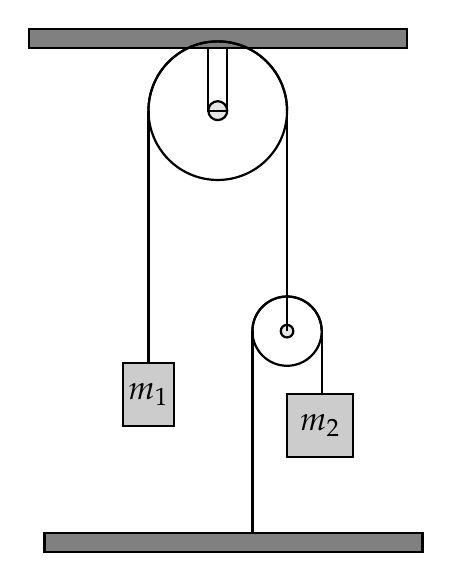
\begin{tikzpicture}[scale=0.8, thick]
    % Ceiling
    \draw[fill=gray] (-3, 6) rectangle (3, 6.3);
    
    % Floor
    \draw[fill=gray] (-2.75, -2) rectangle (3.25, -1.7);
    
    % Top Pulley
    \draw (0, 5) circle (1.1);
    \draw[fill=gray!20] (0, 5) circle (0.15);
    \draw (-0.15, 5) rectangle (0.15, 6); % Mount
    
    % Bottom Pulley
    \draw (1.1, 1.5) circle (0.55);
    \draw[fill=gray!20] (1.1, 1.5) circle (0.1);
    
    % Rope 1 (m1 to bottom pulley axle)
    \draw (-1.1, 5) -- (-1.1, 1);
    \draw (1.1, 5) -- (1.1, 1.5); % Goes to axle of bottom pulley
    \draw (-1.1, 5) arc (180:0:1.1);
    
    % Rope 2 (floor to m2)
    \draw (0.55, -1.7) -- (0.55, 1.5);
    \draw (1.65, 1.5) -- (1.65, 0.5);
    \draw (0.55, 1.5) arc (180:0:0.55);
    
    % Masses
    \draw[fill=gray!40] (-1.5, 0) rectangle (-0.7, 1) node[midway, font=\large] {$m_1$};
    \draw[fill=gray!40] (1.1, -0.5) rectangle (2.15, 0.5) node[midway, font=\large] {$m_2$};

\end{tikzpicture}
\end{center}

Your ultimate task is to answer the following two questions using the 8-step method.
\begin{enumerate}[label=(\alph*)]
    \item What are the accelerations of mass $m_1$ and mass $m_2$?
    \item What is the force on the ceiling?
\end{enumerate}

Begin with step 1: \textbf{Identify special cases for which you can predict the results -- or for which you are uncertain about the results!}

Then do steps 2 through 7. Finally, in step 8, check your predictions from step 1.
\end{exercise}

Then do steps 2 through 7. Finally, in step 8, check your predictions from step 1.
\end{exercise}
\begin{solution}
(a) For mass 1:
\[ T_A - m_1 g = m_1 a_{1y} \]
For mass 2:
\[ T_B - m_2 g = m_2 a_{2y} \]
For the bottom pulley (massless):
\[ T_A - 2T_B = 0 \implies T_A = 2T_B \]
For the top pulley (massless, attached to ceiling):
\[ F_c - 2T_A = 0 \implies F_c = 2T_A \]

Constraint equation: if mass 1 moves down by $y$, rope A pulls the bottom pulley up by $y$. The two vertical segments of rope B each give up $y$ length, meaning mass 2 moves down by $2y$. Taking downward as positive for both masses:
\[ a_{2y} = -2a_{1y} \]

Substituting $T_B = \frac{1}{2}T_A$ and $a_{2y} = -2a_{1y}$ into the mass 2 equation:
\[ \frac{1}{2}T_A - m_2 g = m_2 (-2a_{1y}) \]
Multiply by 2:
\[ T_A - 2m_2 g = -4m_2 a_{1y} \]
Subtract this from the mass 1 equation to eliminate $T_A$:
\[ (T_A - m_1 g) - (T_A - 2m_2 g) = m_1 a_{1y} - (-4m_2 a_{1y}) \]
\[ g(2m_2 - m_1) = a_{1y}(m_1 + 4m_2) \implies a_{1y} = \frac{2m_2 - m_1}{m_1 + 4m_2} g \]
And for mass 2:
\[ a_{2y} = -2a_{1y} = \frac{2m_1 - 4m_2}{m_1 + 4m_2} g \]

(b) To find the force on the ceiling, we first find $T_A$:
\[ T_A = m_1(g + a_{1y}) = m_1 \left( g + \frac{2m_2 - m_1}{m_1 + 4m_2} g \right) = m_1 g \left( \frac{m_1 + 4m_2 + 2m_2 - m_1}{m_1 + 4m_2} \right) = \frac{6m_1 m_2}{m_1 + 4m_2} g \]
The force on the ceiling is:
\[ F_c = 2T_A = \frac{12m_1 m_2}{m_1 + 4m_2} g \]
\end{solution}

% ==================== LECTURE 16 ====================
\chapter{Tension in a Rope; Polar Coordinates}

\section{Tension in a Rope}

A rope with uniform mass density, total mass $m$, and length $\ell$ is attached to a block of mass $M$, which slides on a frictionless surface. The rope is pulled in the $+x$ direction (rightward) with force $F$. Neglect any sagging of the rope due to gravity.

\begin{center}
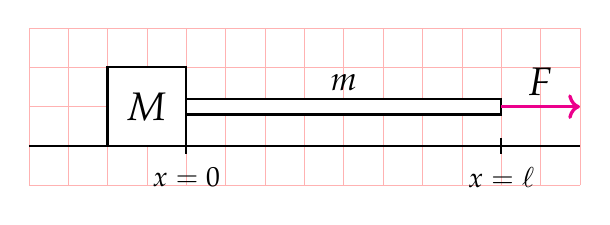
\begin{tikzpicture}[scale=1]
    % Grid
    \draw[step=0.5cm, red!30, very thin] (-0.5, -0.5) grid (6.5, 1.5);
    
    % Surface
    \draw[thick] (-0.5, 0) -- (6.5, 0);
    
    % Block M
    \draw[thick, fill=white] (0.5, 0) rectangle (1.5, 1);
    \node at (1, 0.5) {\Large $M$};
    
    % Rope m
    \draw[thick, fill=white] (1.5, 0.4) rectangle (5.5, 0.6);
    \node at (3.5, 0.8) {\large $m$};
    
    % Force F
    \draw[->, very thick, magenta] (5.5, 0.5) -- (6.5, 0.5) node[midway, above, black] {\Large $F$};
    
    % Labels
    \draw[thick] (1.5, -0.1) -- (1.5, 0.1);
    \node at (1.5, -0.4) {$x=0$};
    
    \draw[thick] (5.5, -0.1) -- (5.5, 0.1);
    \node at (5.5, -0.4) {$x=\ell$};
\end{tikzpicture}
\end{center}

In the exercise below, you will find the tension at various points along the rope for different scenarios. Things to keep in mind for each part:
\begin{itemize}
    \item Clearly indicate the ``system'' you are considering -- e.g., ``block + rope'', or ``only block'', or ``block + part of the rope''.
    \item Label the system with the relevant (total) mass.
    \item Draw a force diagram with only the force vectors acting on the defined system; use precise notation to label each force.
\end{itemize}

\textbf{Question:} What is the ``constraint'' on the accelerations of the block and different parts of the rope? \\
\textcolor{blue}{Acceleration is the same!}

\begin{exercise}[Exercise 1]
Work on your whiteboards for this Exercise.
\begin{enumerate}[label=(\alph*)]
    \item What is the tension $T_R$ at the right end of the rope (the end that is being pulled)? \textit{Hint:} Draw the force diagram for a bit of rope of mass $dm$ at the very end of the rope, write Newton's 2nd Law, and then let $dm \to 0$.
    \item Find an expression for the acceleration of the block plus the rope.
    \item Find an expression for the tension $T_L$ at the left end of the rope (the end attached to the block). When you find the result, check that you get the expected result for an ``ideal rope'' -- i.e., when $m = 0$.
    \item Find an expression for the tension $T(x)$ in the rope at an arbitrary distance $x$ from the block.
    \textit{Hint:} Draw a force diagram for the block plus a piece of the rope of length $x$.
    Check that you get the expected result when $x = 0$ and when $x = \ell$.
    \item What conclusion can you draw about the tension $T(x)$ along the rope when $m = 0$?
    \item Now assume there is \textbf{non-zero friction} $f$ between the block and the surface. On Problem Set 6, you will show that in this case, the tension at the left end of the rope is
    \[ T_L = \frac{M}{M+m} F + \left(1 - \frac{M}{m+M}\right) f. \]
    Check that this result reduces to the expected results for $T_L$ (derived above) when $f = 0$ and when $m = 0$.
    \item Now consider the extreme case of static friction -- i.e., the block does not slip when the force $F$ is applied. What can you conclude about the tensions at the two ends of the rope for this case?
    \item So have we found another condition under which the tension in the rope is the same everywhere along the rope?
\end{enumerate}
\end{exercise}

\begin{solution}
(a) For a small mass chunk $dm$ at the right end, Newton's second law is $F - T_R = dm\, a_x$. As $dm \to 0$, $F - T_R \to 0$, so $T_R = F$.

(b) Treating the block and rope as a single system of mass $(M+m)$:
\[ F = (M+m)a_x \implies a_x = \frac{F}{M+m} \]

(c) Treating just the block as the system, the only horizontal force is $T_L$:
\[ T_L = M a_x = \frac{M}{M+m}F \]
If $m=0$, $T_L = \frac{M}{M}F = F$, which is expected for an ideal massless rope.

(d) Treat the block plus a portion of the rope of length $x$ as the system. The mass is $M + m \frac{x}{\ell}$. The forward force on this system is $T(x)$:
\[ T(x) = \left(M + m\frac{x}{\ell}\right) a_x = \frac{M + m \frac{x}{\ell}}{M+m} F \]
Checks: when $x=0$, $T(0) = \frac{M}{M+m}F = T_L$. When $x=\ell$, $T(\ell) = \frac{M+m}{M+m}F = F = T_R$. Both check out!

(e) When $m=0$, the expression simplifies to $T(x) = \frac{M}{M}F = F$. The tension is the same everywhere.

(f) If $f=0$, it reduces to $T_L = \frac{M}{M+m}F$. If $m=0$, $T_L = F + (1 - 1)f = F$. This checks out!

(g) If the block does not slip, $a_x = 0$. So $T_R = F$. For the whole system, $F - f = 0 \implies f = F$. For the block, $T_L - f = 0 \implies T_L = f = F$. Therefore, $T_R = T_L = F$.

(h) Yes! A rope that is not accelerating ($a_x = 0$) will have uniform tension regardless of its mass.
\end{solution}

\textbf{Final conclusion:} For a horizontal rope (neglecting sag due to gravity), there are two ways to meet the conditions for an `ideal' rope (i.e., the assumption that tension is the same everywhere in the rope): either $m=0$ \textbf{or} $a=0$ (or both).

You will consider the case when gravity plays a role in future activities and problems.

\section{Polar Coordinates}

We will now extend our description of the motion (kinematics) of a point particle in \textbf{two} dimensions from \textbf{Cartesian} coordinates to \textbf{polar} coordinates. Our goal in this lesson is to write $\vec{r}(t)$, $\vec{v}(t) = \frac{d\vec{r}}{dt}$, and $\vec{a}(t) = \frac{d^2\vec{r}}{dt^2}$ in polar coordinates. This will give us the tools to more elegantly describe (and interpret) some very interesting classes of motion!

\begin{exercise}[Exercise 2]
In this first set of questions, you will identify some important similarities and \textit{differences} between basis vectors and components in polar and Cartesian coordinates.

Consider the position vector $\vec{r}(t)$, shown in the figure below, for a point along the particle's trajectory, for a particular time $t$.

\begin{center}
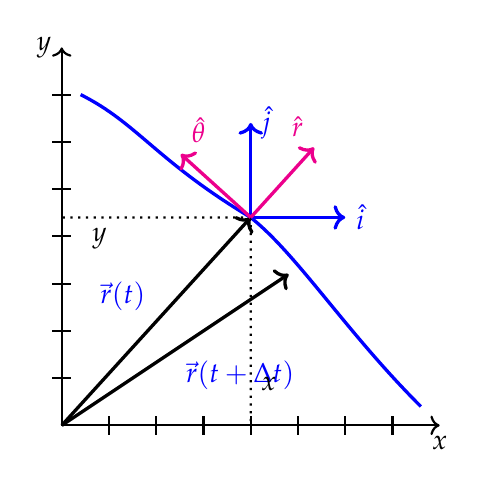
\begin{tikzpicture}[scale=1.2, thick]
    % Axes
    \draw[<->] (0, 4) node[left] {$y$} -- (0, 0) -- (4, 0) node[below] {$x$};
    \foreach \x in {0.5, 1, 1.5, 2, 2.5, 3, 3.5}
        \draw (\x, -0.1) -- (\x, 0.1);
    \foreach \y in {0.5, 1, 1.5, 2, 2.5, 3, 3.5}
        \draw (-0.1, \y) -- (0.1, \y);
    
    % Trajectory
    \draw[blue, very thick] (0.2, 3.5) .. controls (0.8, 3.2) and (1, 2.8) .. (2, 2.2) .. controls (2.5, 1.8) and (3, 1) .. (3.8, 0.2);
    
    % Vectors
    \coordinate (P1) at (2, 2.2);
    \coordinate (P2) at (2.4, 1.6);
    \draw[->, very thick] (0,0) -- (P1) node[midway, above left, blue] {$\vec{r}(t)$};
    \draw[->, very thick] (0,0) -- (P2) node[midway, below right, blue] {$\vec{r}(t+\Delta t)$};
    
    % Projections
    \draw[dotted] (P1) -- (2, 0) node[pos=0.8, right] {$x$};
    \draw[dotted] (P1) -- (0, 2.2) node[pos=0.8, below] {$y$};
    
    % Basis Vectors
    \draw[->, very thick, blue] (P1) -- ++(1, 0) node[right] {$\hat{i}$};
    \draw[->, very thick, blue] (P1) -- ++(0, 1) node[right] {$\hat{j}$};
    \draw[->, very thick, magenta] (P1) -- ++(0.67, 0.74) node[above left] {$\hat{r}$};
    \draw[->, very thick, magenta] (P1) -- ++(-0.74, 0.67) node[above right] {$\hat{\theta}$};
\end{tikzpicture}
\end{center}

\begin{enumerate}[label=(\alph*)]
    \item In a Cartesian coordinate system, the coordinates are $x$ and $y$, and the corresponding orthonormal ``basis vectors'' are $\hat{i}$ and $\hat{j}$. \\
    Because we wish to eventually describe \textit{displacements} $\Delta\vec{r}$ of the particle as it moves along its trajectory, we place the basis vectors at the tip of the position vector -- i.e., at a point along the particle's trajectory. \\
    Label the basis vectors $\hat{i}$ and $\hat{j}$ in the above diagram.
    \item In a polar coordinate system, the polar coordinates are $r$ and $\theta$, and the orthogonal basis vectors are $\hat{r}$ and $\hat{\theta}$.
\end{enumerate}
\end{exercise}

\begin{enumerate}[resume, label=(\alph*)]
    \item In Cartesian coordinates, the position vector is $\vec{r} = x\hat{i} + y\hat{j}$. \\
    In polar coordinates, the position vector is $\vec{r} = $\underline{\textcolor{blue}{\quad $r\hat{r}$ \quad}}.
    \item As a point moves around in the plane with time, do the Cartesian basis vectors describing $\vec{r}(t)$ ever change with time? \\
    \textcolor{blue}{No.}
    \item Can either or both of the polar basis vectors change with position along the trajectory, and therefore change with time? \\
    \textcolor{blue}{Yes.}
    \item For what type of motion will each of the polar \textbf{coordinates} \textit{not} change with time?
    \begin{itemize}
        \item \textcolor{blue}{$\theta = \text{constant}$ $\implies$ motion along a straight line passing through the origin.}
        \item \textcolor{blue}{$r = \text{constant}$ $\implies$ motion in a circle centered on the origin.}
    \end{itemize}
    \item For what type(s) of motion will one or both of the polar \textbf{basis vectors} \textit{not} change with time? \\
    \textcolor{blue}{Motion along a straight line passing through the origin.}
    \[ \implies \hat{r} = \hat{r}(\theta), \quad \hat{\theta} = \hat{\theta}(\theta). \]
\end{enumerate}

We can now write $\vec{r} = r\hat{r}$ in polar coordinates making dependencies of each factor explicit:
\[ \vec{r} = r\hat{r}(\theta) \quad \text{or, making the time dependence explicit,} \quad \vec{r}(t) = r(t)\hat{r}(\theta(t)) \]

In polar coordinates, the position vector $\vec{r}$ looks very simple! However, taking the derivative with respect to time gets more complicated since $\hat{r}$ depends on the coordinate $\theta$, and all of the quantities $\{r, \theta, \hat{r}(\theta), \hat{\theta}(\theta)\}$ can depend on the position along the trajectory, and therefore on time! Nevertheless, we'll plunge on and derive $\vec{v}(t) = d\vec{r}/dt$.

\begin{exercise}[Exercise 3]
Follow these steps to find the velocity vector in polar coordinates.
\begin{enumerate}[label=(\alph*)]
    \item Apply the product rule and then move on to the next step:
    \[ \vec{v} = \frac{d\vec{r}}{dt} = \frac{d}{dt}(r\hat{r}(\theta)) = \textcolor{blue}{\frac{dr}{dt}\hat{r}(\theta) + r\frac{d\hat{r}(\theta)}{dt}} \]
    \item Draw a pair of Cartesian basis vectors $\hat{i}$ and $\hat{j}$, and a pair of polar basis vectors $\hat{r}$ and $\hat{\theta}$ (centered on the same point), with the angle $\theta$ carefully indicated. Write expressions for $\hat{r}(\theta)$ and $\hat{\theta}(\theta)$ in terms of $\hat{i}$, $\hat{j}$, and $\theta$.
    
    \textcolor{blue}{
    \begin{align*}
        \hat{r} &= \cos\theta\,\hat{i} + \sin\theta\,\hat{j} \\
        \hat{\theta} &= -\sin\theta\,\hat{i} + \cos\theta\,\hat{j}
    \end{align*}
    }
    \textit{Check that your polar basis vectors are orthogonal! How?} \\
    \textcolor{blue}{Take the dot product: $\hat{r} \cdot \hat{\theta} = -\sin\theta\cos\theta + \sin\theta\cos\theta = 0$.}
    
    \item Differentiate (with respect to time) the expression you just found for $\hat{r}$ to show that
    \[ \frac{d\hat{r}}{dt} = \frac{d\theta}{dt}\hat{\theta}. \]
    \textit{Hint:} You may need to use the chain rule.
    \item Interpret your result geometrically -- i.e., draw a picture. For example, draw the basis vector $\hat{r}$ for position vector $\vec{r}(t)$ and then for $\vec{r}(t+\Delta t) = \vec{r} + \Delta\vec{r}$. What is the change in $\hat{r}$?
    \item Use the result for $d\hat{r}/dt$ from (c) to write the velocity (from (a)) in polar coordinates:
    \[ \vec{v} = \frac{d\vec{r}}{dt} = \textcolor{blue}{\frac{dr}{dt}\hat{r} + r\frac{d\theta}{dt}\hat{\theta}} \label{eq:v_polar} \tag{2} \]
    \item Write a simple equation expressing each of the following conditions, and then use eq. \ref{eq:v_polar} to write the corresponding form of $\vec{v} = d\vec{r}/dt$. Check that your result is consistent with the fact that $\vec{v}$ must be tangent to the particle's trajectory.
    \begin{enumerate}[label=(\roman*)]
        \item Motion in a circle centered on the origin. \\
        Condition: \textcolor{blue}{$r = \text{constant} \implies dr/dt = 0$} \\
        $\implies \vec{v} =$ \textcolor{blue}{$r\frac{d\theta}{dt}\hat{\theta}$} \\
        Tangent? \textcolor{blue}{Yes.}
        \item Motion along a straight line, passing through the origin. \\
        Condition: \textcolor{blue}{$\theta = \text{constant} \implies d\theta/dt = 0$} \\
        $\implies \vec{v} =$ \textcolor{blue}{$\frac{dr}{dt}\hat{r}$} \\
        Tangent? \textcolor{blue}{Yes.}
    \end{enumerate}
    \item Make a sketch of a particle's trajectory on a graph of $y$ vs. $x$. At a point on the trajectory where $\vec{v}$ has non-zero $\hat{r}$ and $\hat{\theta}$ components, illustrate the interpretation of each term in $\vec{v}$ by considering the polar components of a displacement $\Delta\vec{r}$ along the trajectory.
\end{enumerate}

\textbf{Summary:} In polar coordinates, the velocity vector has two terms, which describe the velocity in the $\hat{r}$ and $\hat{\theta}$ directions:
\[ \vec{v} = \frac{d\vec{r}}{dt} = \frac{dr}{dt}\hat{r} + r\frac{d\theta}{dt}\hat{\theta}. \]
\end{exercise}

\begin{solution}
(c) Using the chain rule:
\[ \frac{d\hat{r}}{dt} = \frac{d}{dt}(\cos\theta\,\hat{i} + \sin\theta\,\hat{j}) = \frac{d\theta}{dt}(-\sin\theta\,\hat{i} + \cos\theta\,\hat{j}) = \frac{d\theta}{dt}\hat{\theta} \]

(d) The difference $\Delta\hat{r}$ between $\hat{r}(t+\Delta t)$ and $\hat{r}(t)$ points perpendicular to $\hat{r}$, which is precisely the $\hat{\theta}$ direction!

(g) Diagram for displacement $\Delta\vec{r}$:
\begin{center}
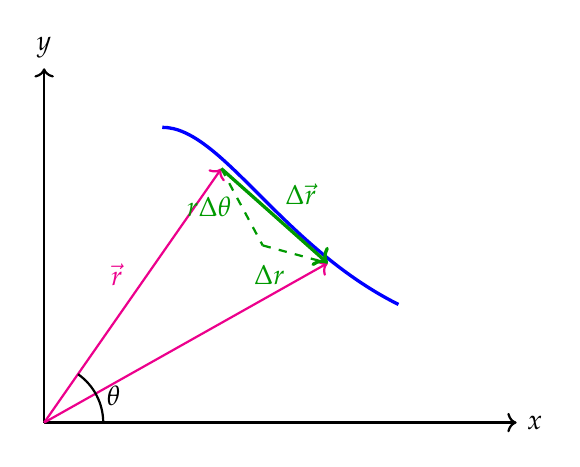
\begin{tikzpicture}[scale=1.5, thick]
    \draw[->] (0, 0) -- (4, 0) node[right] {$x$};
    \draw[->] (0, 0) -- (0, 3) node[above] {$y$};
    
    \draw[blue, very thick] (1, 2.5) .. controls (1.5, 2.5) and (2, 1.5) .. (3, 1);
    
    \coordinate (P1) at (1.5, 2.15);
    \coordinate (P2) at (2.4, 1.35);
    
    \draw[->, magenta] (0,0) -- (P1) node[midway, above left] {$\vec{r}$};
    \draw[->, magenta] (0,0) -- (P2);
    
    \draw[->, green!60!black, very thick] (P1) -- (P2) node[midway, above right] {$\Delta\vec{r}$};
    
    \coordinate (P_proj) at (1.85, 1.5);
    \draw[dashed, green!60!black] (P1) -- (P_proj) node[midway, left] {$r\Delta\theta$};
    \draw[dashed, green!60!black] (P_proj) -- (P2) node[midway, below left] {$\Delta r$};
    
    \draw (0.5, 0) arc (0:55:0.5) node[midway, right] {$\theta$};
\end{tikzpicture}
\end{center}
\[ \frac{\Delta\vec{r}}{\Delta t} \approx \frac{\Delta r}{\Delta t}\hat{r} + r\frac{\Delta\theta}{\Delta t}\hat{\theta} \]
\end{solution}

\begin{exercise}[Exercise 4]
We'll now explore the acceleration vector in polar coordinates. We'll outline the process here; you will do the detailed derivation on Problem Set 6.
\begin{enumerate}[label=(\alph*)]
    \item Given that $\vec{a} = \frac{d\vec{v}}{dt}$ and $\vec{v} = \frac{dr}{dt}\hat{r} + r\frac{d\theta}{dt}\hat{\theta}$, how many terms do you expect to get when you differentiate $\vec{v}$? \\
    \textcolor{blue}{5 terms.}
    \item On your problem set, after you use the result you found earlier for $d\hat{r}/dt$, and a similar result for $d\hat{\theta}/dt$, you will find that two of the \textit{five} terms can be combined to give a result that is \textit{almost} identical to the expression in eq. \ref{eq:a_polar} below, in which we have \textit{deliberately left out exactly two symbols or numbers!} \\
    What are the two missing symbols or numbers in this equation?
    \[ \vec{a} = \frac{d\vec{v}}{dt} = \left(\frac{d^2 r}{dt^2} - r\left(\frac{d\theta}{dt}\right)^{\textcolor{red}{\mathbf{2}}}\right)\hat{r} + \left(r\frac{d^2\theta}{dt^2} + \textcolor{red}{\mathbf{2}}\frac{dr}{dt}\frac{d\theta}{dt}\right)\hat{\theta}. \label{eq:a_polar} \tag{3} \]
    \item Write the equations expressing each of the following conditions, and then write the corresponding form of $\vec{a}$ in polar coordinates -- i.e., a simpler form of eq. \ref{eq:a_polar} for each case. Try to interpret each term in your expression for $\vec{a}$.
    \begin{enumerate}[label=(\roman*)]
        \item Motion in a circle centered on the origin. \\
        \textcolor{blue}{
        \[ \vec{a} = -r\left(\frac{d\theta}{dt}\right)^2\hat{r} + r\frac{d^2\theta}{dt^2}\hat{\theta} \]
        }
        \item Motion along a straight line, passing through the origin. \\
        \textcolor{blue}{
        \[ \vec{a} = \frac{d^2r}{dt^2}\hat{r} \]
        }
    \end{enumerate}
    \item Now try to interpret all four terms in the expression for $\vec{a}$ -- i.e., how would you describe each type of acceleration?
    \[ \vec{a} = \left( \underbrace{\frac{d^2 r}{dt^2}}_{\textcolor{blue}{\text{radial}}} - \underbrace{r\left(\frac{d\theta}{dt}\right)^2}_{\textcolor{blue}{\text{centripetal}}} \right)\hat{r} + \left( \underbrace{r\frac{d^2\theta}{dt^2}}_{\textcolor{blue}{\text{tangential}}} + \underbrace{2\frac{dr}{dt}\frac{d\theta}{dt}}_{\textcolor{blue}{\text{Coriolis}}} \right)\hat{\theta} \]
    Question: Which term (if any) in each component must \textit{always} have the same sign -- i.e., which are always positive or always negative? Interpret the sign. \\
    \textcolor{blue}{The centripetal term $-r(d\theta/dt)^2$ is always negative, meaning it always points radially inward (towards the origin).}
\end{enumerate}
\end{exercise}

% ==================== LECTURE 17 ====================
\chapter{Angular Kinematics; Conical Pendulum}

\begin{exercise}[Exercise 1]
In the two left columns of the table below, you are given the name, symbol, and defining equation for kinematic quantities in 1D, where the 1D coordinate is \textbf{position} $x$. For descriptions of translational motion, we use roman symbols, like $x, v_x, a_x$.

In the rightmost column, write the analogous equations for the case when the 1D coordinate is the \textbf{polar angle} $\theta$. For descriptions of angular motion, we often use Greek letters. Can you recall what the standard symbols are for these angular kinematic variables (for example, if you have encountered them in high school or other courses)?

\begin{table}[h!]
\centering
\caption{Kinematic variables in 1D. Angular kinematic variables and dimensions.}
\renewcommand{\arraystretch}{1.5}
\begin{tabular}{|c|c||c|c|c|}
\hline
Name & Symbol/Definition & Name & Symbol/Definition & Dimensions \\ \hline
1D position & $x$ & angular position & \textcolor{blue}{$\theta$} & \textcolor{blue}{$1$} \\ \hline
displacement & $\Delta x \equiv x_2 - x_1$ & angular displacement & \textcolor{blue}{$\Delta\theta$} & \textcolor{blue}{$1$} \\ \hline
velocity & $v_x \equiv \frac{dx}{dt}$ & angular velocity & \textcolor{blue}{$\omega \equiv \frac{d\theta}{dt}$} & \textcolor{blue}{$T^{-1}$} \\ \hline
acceleration & $a_x \equiv \frac{dv_x}{dt} = \frac{d^2x}{dt^2}$ & angular acceleration & \textcolor{blue}{$\alpha \equiv \frac{d\omega}{dt} = \frac{d^2\theta}{dt^2}$} & \textcolor{blue}{$T^{-2}$} \\ \hline
\end{tabular}
\end{table}
\end{exercise}

\begin{exercise}[Exercise 2]
Now rewrite the equations you derived in Lecture 16 for $\vec{v}$ and $\vec{a}$ for the special case of \textit{motion in a circle centered on the origin} (already entered on the left side of Table 2 below) using the angular variables you defined in Table 1. Check that the dimensions of each term are consistent with expectations.

\begin{table}[h!]
\centering
\caption{Velocity and acceleration in polar coordinates for \textit{motion in a circle centered on the origin}.}
\renewcommand{\arraystretch}{2}
\begin{tabular}{|c|c||c|}
\hline
Name & From Lecture 16 & In terms of Greek symbols \\ \hline
velocity & $\vec{v} = r\frac{d\theta}{dt}\hat{\theta}$ & \textcolor{blue}{$\vec{v} = r\omega\hat{\theta}$} \\ \hline
acceleration & $\vec{a} = -r\left(\frac{d\theta}{dt}\right)^2\hat{r} + r\frac{d^2\theta}{dt^2}\hat{\theta}$ & \textcolor{blue}{$\vec{a} = -r\omega^2\hat{r} + r\alpha\hat{\theta}$} \\ \hline
\end{tabular}
\end{table}
\end{exercise}

\textbf{From polar to cylindrical coordinates:}

We can extend polar coordinates to three dimensions by adding one more coordinate axis: e.g., the $z$ axis. Our coordinates are then $r$, $\theta$, and $z$, and the corresponding basis vectors are $\hat{r}$, $\hat{\theta}$, and $\hat{k}$ (or $\hat{z}$). We'll use this coordinate system in the next exercise.

\begin{exercise}[Exercise 3: The Conical Pendulum]
Consider a mass $M$ fixed to the bottom end of a rod of length $\ell$ and negligible mass, as shown in the drawing below. The top end of the rod can pivot about a pin in a hub. The hub rotates at constant angular speed $\omega$. The mass moves with steady speed in a circular path of constant radius $r$. In this Exercise, you will find the angle $\alpha$ that the rod makes with the vertical, and carefully interpret your results to discover an interesting physical phenomenon, which forms the basis of operation of the ``centrifugal governor''.

\begin{center}
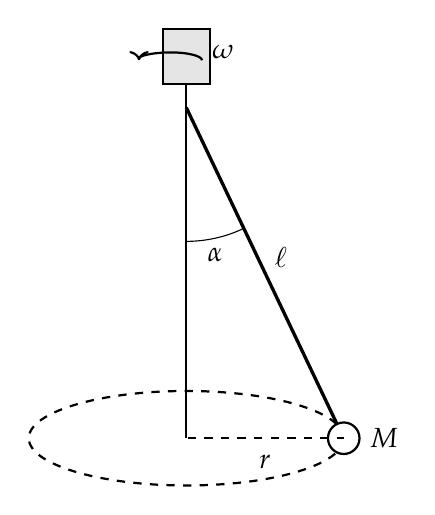
\begin{tikzpicture}[scale=1]
    % Axes
    \draw[->, thick] (0, 0) -- (0, 5) node[right] {$z$};
    
    % Circle
    \draw[dashed, thick] (0, 0) ellipse (2cm and 0.6cm);
    
    % Hub
    \draw[thick, fill=gray!20] (-0.3, 4.5) rectangle (0.3, 5.2);
    \draw[thick] (0, 4.5) -- (0, 4.2);
    \draw[->, thick] (0.2, 4.8) arc (0:180:0.4 and 0.1) node[midway, right=4mm] {$\omega$};
    
    % Pendulum
    \draw[very thick] (0, 4.2) -- (2, 0);
    \draw[fill=white, thick] (2, 0) circle (0.2) node[right=2mm] {$M$};
    
    % Dashed line to center
    \draw[dashed, thick] (0, 4.2) -- (0, 0) -- (2, 0);
    
    % Labels
    \node at (1, -0.3) {$r$};
    \node at (1.2, 2.3) {$\ell$};
    \draw (0, 2.5) arc (-90:-65:1.7) node[midway, below] {$\alpha$};
\end{tikzpicture}
\end{center}

\begin{enumerate}[label=(\alph*)]
    \item What would you expect the behaviour of this pendulum to be for increasing values of the angular speed $\omega$, starting from $\omega = 0$? \\
    \textcolor{blue}{It goes up (angle $\alpha$ increases).}
    
    \item On your whiteboard, sketch two graphs that illustrate your expectation.
    \begin{itemize}
        \item In the first graph, plot your expectation for $\alpha$ versus $\omega$.
        \item In the second graph, plot $\cos\alpha$ versus $\omega$.
    \end{itemize}
    \textcolor{blue}{We expect $\alpha$ to start at 0 and approach $\pi/2$ as $\omega \to \infty$. We expect $\cos\alpha$ to start at 1 and approach 0 as $\omega \to \infty$.}
    
    \item On your whiteboard, draw the force diagram for the mass. \\
    \textcolor{blue}{The forces on $M$ are tension $T$ directed up along the rod, and gravity $Mg$ directed downwards.}
    
    \item Define an appropriate coordinate system. Then write Newton's 2nd Law for each of the relevant coordinates. \\
    \textcolor{blue}{Using polar/cylindrical coordinates ($r, z$). Note that $r = \ell\sin\alpha$.
    \begin{align*}
        z&: \quad T\cos\alpha - Mg = 0 \quad \text{(since $a_z = 0$)} \\
        r&: \quad -T\sin\alpha = M a_r = M(-r\omega^2) = -M\omega^2(\ell\sin\alpha)
    \end{align*}
    }
    
    \item Find an expression for tension $T$ in terms of quantities you are given ($M$ and $\ell$), and the angular speed $\omega$.
    \textit{Hint:} If there are too many ``unknowns'', consider whether $r, \ell$, and $\sin\alpha$ are all independent. If they are not, how are they related? \\
    \textcolor{blue}{From the radial equation, assuming $\sin\alpha \neq 0$:
    \[ T\sin\alpha = M\ell\omega^2\sin\alpha \implies T = M\ell\omega^2 \]
    }
    
    \item Find an expression for $\cos\alpha$. \\
    \textcolor{blue}{Substituting $T$ into the $z$-equation:
    \[ (M\ell\omega^2)\cos\alpha = Mg \implies \cos\alpha = \frac{g}{\ell\omega^2} \]
    }
    
    \item Consider the special or limiting cases for $\omega$ in the order described below. Discuss whether your prediction for $\alpha$ makes physical sense for each limiting case.
    \begin{enumerate}[label=(\roman*)]
        \item Start with the case when $\omega^2 \gg \frac{g}{\ell}$ or $\omega \gg \sqrt{\frac{g}{\ell}}$. \\
        \textcolor{blue}{Then $\cos\alpha \to 0 \implies \alpha \to \frac{\pi}{2}$. This makes sense; at very high speeds, the pendulum flies out horizontally.}
        \item Then consider the limiting case $\omega \to 0$. Do we have an issue? What might be the culprit? (Spend a minute thinking about this and then move on to get some hints.) \\
        \textcolor{blue}{As $\omega \to 0$, $\cos\alpha \to \infty$, which is impossible! $\cos\alpha$ must be $\le 1$.}
    \end{enumerate}
    
    \item On your whiteboard, make a sketch of the expression you found for $\cos\alpha$ [in part (f)] as a function of $\omega$ -- i.e., plot $g/(\ell\omega^2)$ versus $\omega$.
    Is there \textit{another} special case for $\omega$ that we should consider? Discuss what could happen at angular frequencies above or below this value.
    \textit{Hint:} It may be helpful to consider carefully the case when $\cos\alpha = 1$. For what value of $\alpha$ is $\cos\alpha = 1$? \\
    \textcolor{blue}{$\cos\alpha = 1$ when $\alpha = 0$. This occurs at a critical angular frequency $\omega_c = \sqrt{g/\ell}$. Below this frequency, the equation yields non-physical results.}
    
    \item Go back to the expressions you wrote in part (d) for Newton's 2nd Law. Is there another possible solution to the equations, that is true for \textit{all} values of $\omega$? How does this help resolve the issue in the previous subpart?
    \textit{Hint:} Consider the case when the pendulum hangs straight down\dots What is the value of $\sin\alpha$? \\
    \textcolor{blue}{If the pendulum hangs straight down, $\alpha = 0$ and $\sin\alpha = 0$.
    The $r$-equation $T\sin\alpha = M\ell\omega^2\sin\alpha$ becomes $0 = 0$, which is true for \textit{any} $\omega$.
    The $z$-equation gives $T\cos(0) = Mg \implies T = Mg$.
    So $\alpha = 0$ is a valid solution!}
    
    \item Now go back and remake your plot of $\cos\alpha$ versus $\omega$ in part (b). \\
    \textcolor{blue}{For $\omega \le \sqrt{g/\ell}$, the pendulum hangs straight down ($\alpha = 0 \implies \cos\alpha = 1$). For $\omega > \sqrt{g/\ell}$, it swings out and $\cos\alpha = \frac{g}{\ell\omega^2}$. The graph of $\cos\alpha$ is a flat horizontal line at 1 until $\omega = \sqrt{g/\ell}$, at which point it decays as $1/\omega^2$.}
\end{enumerate}
\end{exercise}

Historical note: The ``conical pendulum'' is the physics that controls an important mechanical device called the centrifugal governor.
\begin{itemize}
    \item Centrifugal governors were invented by Christiaan Huygens and used to regulate the distance and pressure between millstones in windmills in the 17th century.
    \item In 1788, James Watt adapted one to control his steam engine: the centrifugal governor regulated the admission of steam into the cylinder(s), a development that proved so important that Watt is sometimes called the inventor of the centrifugal governor.
\end{itemize}

See, for example, this Youtube video for a governor in action as a feedback and control system: \url{https://www.youtube.com/watch?v=ASIl3HWTT4U}. However, be wary of the narrator's reference to ``centrifugal force''. There is no such thing as a centrifugal force -- it is ``ficticious''! There are only \textit{real} forces -- in this case, tension and gravity; the net real force inwards is related to the centripetal acceleration, as you wrote in part (d) above.

% ==================== LECTURE 18 ====================
\chapter{Differential Equations in Mechanics - I}

Reading: Sections 3.5 \& 3.6 in Kleppner \& Kolenkow.

Up to this point we have considered only forces that are \textit{constant} or depend (only) on \textit{time}, so that application of Newton's 2nd Law leads to an \textit{algebraic} equation for the acceleration of each mass:
\[ m\vec{a}(t) = \sum_i \vec{F}_i^{\text{ext}}(t). \tag{1} \]
We could then use the general kinematic equations to find velocities and positions:
\begin{align*}
    &\vec{a}(t) \text{ is given or is a solution to an algebraic equation.} \\
    &\vec{v}(t) = \vec{v}(t_0) + \int_{t_0}^t \vec{a}(t')dt' \tag{2} \\
    &\vec{r}(t) = \vec{r}(t_0) + \int_{t_0}^t \vec{v}(t')dt'
\end{align*}

However, these equations are insufficient when the forces (and therefore accelerations) are directly dependent on position and/or velocity: $\vec{F}\left(\vec{r}, \frac{d\vec{r}}{dt}, t\right) = m\,\vec{a}\left(\vec{r}, \frac{d\vec{r}}{dt}, t\right)$.

\textcolor{blue}{\textbf{Quick Question 1:} Why are the above equations insufficient in these cases?} \\
\textcolor{blue}{Because forces depend on position and/or velocity, you can't simply integrate acceleration with respect to time without already knowing the position or velocity over time.}

Since almost all forces \textbf{do} depend on position and/or velocity, this is an important issue!

\textcolor{blue}{\textbf{Quick Question 2:} Can you identify some examples where $\vec{F}$ depends on position or on velocity?} \\
\textcolor{blue}{Position-dependent: gravitational, electrostatic, spring forces. Velocity-dependent: drag forces.}

In this more general scenario, Newton's 2nd Law becomes a \textit{differential equation} for $\vec{r}(t)$,
\[ m\frac{d^2\vec{r}}{dt^2} = \vec{F}\left(\vec{r}, \frac{d\vec{r}}{dt}, t\right), \tag{3} \]
which we must solve in order to find the behavior of our system\footnote{The set of equations arising from Newton's 2nd Law together with any constraints are commonly referred to as the ``equations of motion,'' especially in the situation where they are differential equations.}.

\begin{itemize}
    \item PHYSICS 61 is \textit{not} a course on differential equations, which would take an entire quarter or more (see MATH 53 or MATH 63CM; PHYSICS 111, MATH 131P or MATH 173).
    \item Our goal today will be to identify several common differential equations that arise in mechanics, and various techniques for solving those and similar equations that you will likely encounter many times in physics and/or engineering.
\end{itemize}

In the next two lectures, we will consider a few examples that illustrate three different techniques for solving ordinary differential equations (ODEs).

\section*{Example \& Technique \#1: Drag force --- Separate \& Integrate}

In general, drag forces are quite complicated, and result from complex interactions between the surface of an object and a surrounding fluid (liquid or gas). However, in certain cases drag forces are well-described by simple equations. Here we will consider \textbf{viscous drag,} which applies when turbulence can be neglected; the viscous drag force $\vec{F}_v$ is directly proportional to the velocity of an object through the surrounding fluid:
\[ \vec{F}_v = -C\vec{v}, \tag{4} \]
where $C$ is a \textit{dimensionful} constant of proportionality.
\begin{itemize}
    \item $C$ is defined to be \textit{positive} so that the above vector equation defines a force that always opposes motion, as expected for drag.
    \item In principle $C$ can be computed from the properties of the fluid (density, viscosity) and the geometry of the object (surface area, shape), but we will just assume that $C$ is given (e.g., as the result of an experimental measurement).
\end{itemize}

\begin{exercise}[Exercise 1]
Suppose a particle starts at $x = 0$ with some initial velocity $v_x(t = 0) = v_{x0}$ and is subject to only one force: viscous drag.
\begin{enumerate}[label=(\alph*)]
    \item Write Newton's 2nd Law for the system in terms of only $x(t)$ and/or its derivatives (as in Eq. 3 above). \\
    \textcolor{blue}{
    Given $x(0) = 0$ and $v_x(0) = v_{x0}$,
    \[ F_v = -C\frac{dx}{dt} = m\frac{d^2x}{dt^2} \implies -Cv_x = m\frac{dv_x}{dt} \]
    }
    \item The `order' of a differential equation is the largest number of derivatives in any term. What is the order of the differential equation you wrote in (a)? \\
    \textcolor{blue}{2nd order (since it involves $d^2x/dt^2$).}
    \item The equation you wrote in (a) can be rewritten as a \textit{first-order} differential equation in a different dependent variable -- i.e., rather than the dependent variable $x(t)$, use \dots which variable? \\
    \textcolor{blue}{Velocity $v_x(t)$.} \\
    Write a first-order differential equation for this new dependent variable. \\
    \textcolor{blue}{
    \[ -C v_x = m\frac{dv_x}{dt} \]
    }
    \item Now that we have a first-order differential equation, one technique we can try is \textit{separate and integrate}:
    \begin{itemize}
        \item separate the dependent (\textcolor{blue}{$v_x$}) and independent (\textcolor{blue}{$t$}) variables so that the dependent variable is on only one side of the equation;
        \item then integrate over the independent variable to eliminate the derivative.
    \end{itemize}
\end{enumerate}

Start by moving any factors involving the dependent variable to the lefthand side and everything else to the righthand side:
\[ \underbrace{\frac{1}{v_x}\frac{dv_x}{dt}}_{v_x-\text{dependent}} = \underbrace{-\frac{C}{m}}_{t-\text{dependent (or constant)}} \]
\textcolor{blue}{Now multiply each side by $dt'$ \& integrate -- include limits of integration!}
\textcolor{blue}{
\begin{align*}
    \int_{0}^{t} \frac{1}{v_x(t')} \frac{dv_x}{dt'} dt' &= \int_{0}^{t} -\frac{C}{m} dt' \\
    \int_{v_{x0}}^{v_x(t)} \frac{1}{v_x'} dv_x' &= -\frac{C}{m} t \\
    \ln\left(\frac{v_x(t)}{v_{x0}}\right) &= -\frac{C}{m} t \\
    \implies v_x(t) &= v_{x0}e^{-\frac{C}{m}t}
\end{align*}
}

Check two relevant limiting cases. (Express them as dimensionally consistent limiting cases.) \\
\textcolor{blue}{As $t \to 0$, $v_x(t) \to v_{x0}$. As $t \to \infty$, $v_x(t) \to 0$. Both make physical sense.}

\begin{enumerate}[label=(\alph*), resume]
    \item Sketch $v_x(t)$ as a function of $t$, for $v_{x0} > 0$ and for $v_{x0} < 0$. Label intercepts. Interpret each case. \\
    Add a dimensionally consistent time scale on the $t$ axis, expressed in terms of appropriate dimensionful quantities. Interpret this time and the value of $v_x$ at this time.
    
    \begin{center}
    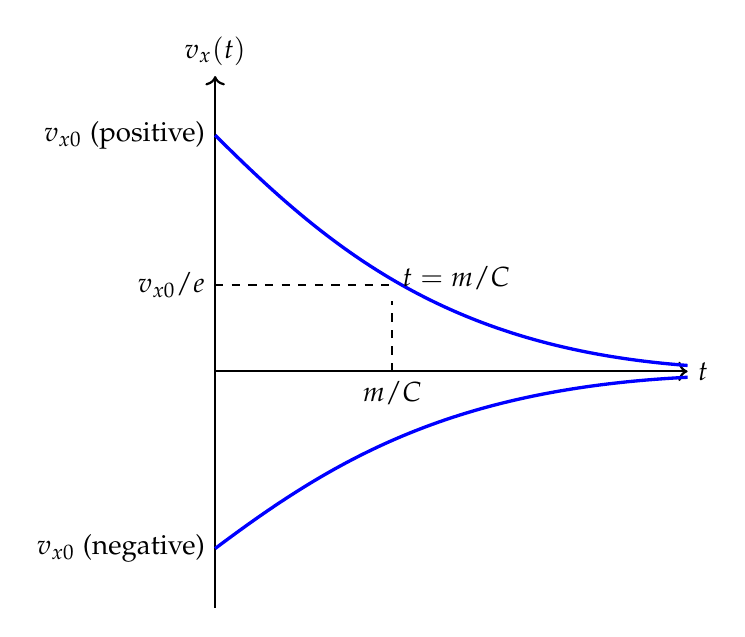
\begin{tikzpicture}[scale=1.5, thick]
        % Axes
        \draw[->] (0, -2) -- (0, 2.5) node[above] {$v_x(t)$};
        \draw[->] (0, 0) -- (4, 0) node[right] {$t$};
        
        % Curves
        \draw[blue, very thick] (0, 2) .. controls (1, 1) and (2, 0.2) .. (4, 0.05);
        \draw[blue, very thick] (0, -1.5) .. controls (1, -0.75) and (2, -0.15) .. (4, -0.05);
        
        % Labels
        \node[left] at (0, 2) {$v_{x0}$ (positive)};
        \node[left] at (0, -1.5) {$v_{x0}$ (negative)};
        
        % Time constant
        \draw[dashed] (1.5, 0) -- (1.5, 0.6) node[above right] {$t = m/C$};
        \node[below] at (1.5, 0) {$m/C$};
        \draw[dashed] (0, 0.73) node[left] {$v_{x0}/e$} -- (1.5, 0.73);
    \end{tikzpicture}
    \end{center}
    \textcolor{blue}{The velocity decays exponentially towards zero. The characteristic time scale is $\tau = m/C$, which is the time it takes for the velocity to decrease by a factor of $1/e$.}
\end{enumerate}

Once we have an equation for velocity in terms of (only) time, we can directly integrate to find the position using equation 2. We won't do the math here.
\end{exercise}

\begin{exercise}[Exercise 2]
Now repeat this derivation for a particle \textit{falling} through a viscous fluid -- i.e., subject to \textit{both} viscous drag and gravity. Start by defining a coordinate system with the positive $y$ direction pointing up.
\begin{enumerate}[label=(\alph*)]
    \item Draw a picture of the situation. Then use Newton's 2nd Law to write the differential equation for $v_y(t)$. \\
    \textcolor{blue}{
    Let $+y$ point upwards. Gravity acts downwards ($-mg$). Drag opposes velocity ($-C v_y$).
    \[ m\frac{dv_y}{dt} = -Cv_y - mg \label{eq:drag_grav} \tag{5} \]
    }
    Is your equation valid for both positive and negative values of $v_y(t)$? \\
    \textcolor{blue}{Yes. If $v_y > 0$ (moving up), drag is $-Cv_y < 0$ (down). If $v_y < 0$ (moving down), drag is $-Cv_y > 0$ (up).}
    
    \item Now separate and integrate. But think carefully about how to do this -- recall that we needed the entire $v$-dependent side to include an overall factor of $\frac{dv}{dt}$ for the separation of variables to work. \\
    \textit{Hint:} Try defining $u_y(t) \equiv v_y(t) + k$, where $k$ is a constant. What should $k$ be? What is $\frac{du_y}{dt}$? \\
    \textcolor{blue}{
    Rewrite the differential equation:
    \[ m\frac{dv_y}{dt} = -C\left(v_y + \frac{mg}{C}\right) \]
    Define $u_y(t) = v_y(t) + \frac{mg}{C}$. Then $k = \frac{mg}{C}$ and $\frac{du_y}{dt} = \frac{dv_y}{dt}$.
    The equation becomes:
    \[ m\frac{du_y}{dt} = -Cu_y \implies \frac{1}{u_y}\frac{du_y}{dt} = -\frac{C}{m} \]
    Separating and integrating yields $u_y(t) = u_{y0} e^{-\frac{C}{m}t}$.
    Substituting back $v_y$:
    \[ v_y(t) + \frac{mg}{C} = \left(v_{y0} + \frac{mg}{C}\right)e^{-\frac{C}{m}t} \implies v_y(t) = \left(v_{y0} + \frac{mg}{C}\right)e^{-\frac{C}{m}t} - \frac{mg}{C} \]
    }
    Check the relevant limiting cases. \\
    \textcolor{blue}{As $t \to \infty$, $v_y(t) \to -mg/C$. This is the terminal velocity.}
    
    \item Sketch $v_y(t)$ as a function of $t$ for initial velocity $v_{y0}$ in certain ranges -- which ranges? \\
    Identify and provide a physical interpretation for \textit{three} different ranges of $v_{y0}$. \\
    Also interpret the physical significance of $v_y(t) = 0$ -- if it occurs.
    
    \begin{center}
    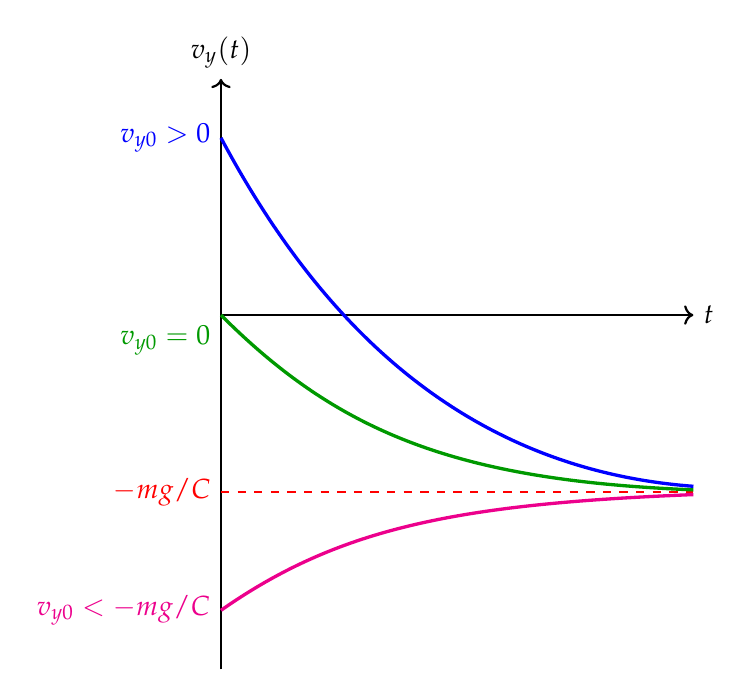
\begin{tikzpicture}[scale=1.5, thick]
        % Axes
        \draw[->] (0, -3) -- (0, 2) node[above] {$v_y(t)$};
        \draw[->] (0, 0) -- (4, 0) node[right] {$t$};
        
        % Terminal velocity asymptote
        \draw[dashed, red] (0, -1.5) node[left] {$-mg/C$} -- (4, -1.5);
        
        % Curve 1: v_y0 > 0
        \draw[blue, very thick] (0, 1.5) node[left] {$v_{y0} > 0$} .. controls (0.8, 0) and (2, -1.3) .. (4, -1.45);
        
        % Curve 2: v_y0 = 0
        \draw[green!60!black, very thick] (0, 0) node[below left] {$v_{y0} = 0$} .. controls (1, -1) and (2, -1.4) .. (4, -1.48);
        
        % Curve 3: v_y0 < -mg/C
        \draw[magenta, very thick] (0, -2.5) node[left] {$v_{y0} < -mg/C$} .. controls (1, -1.8) and (2, -1.6) .. (4, -1.52);
    \end{tikzpicture}
    \end{center}
    \textcolor{blue}{
    1. $v_{y0} > 0$: Thrown upwards. Reaches $v_y = 0$ (highest point), then falls and approaches terminal velocity. \\
    2. $v_{y0} = 0$: Dropped from rest. Accelerates downwards, asymptotically approaching terminal velocity. \\
    3. $v_{y0} < -mg/C$: Thrown downwards faster than terminal velocity. Slows down (decelerates) upwards until it reaches terminal velocity.
    }
\end{enumerate}
\end{exercise}

% ==================== LECTURE 19 ====================
\chapter{Differential Equations in Mechanics - II}
\textbf{Extended objects --- Setting up a differential equation}

There are cases in mechanics where differential equations show up -- but \textit{not} as equations of motion. In these cases we generally have to carefully analyze a situation in order to determine which equation to even solve\dots The equation can often be determined by considering a tiny (`infinitesimal' or `differential') piece of the system. As an example, we'll calculate the tension in a whirling rope with a mass at the end of the rope:
\begin{itemize}
    \item Consider an object of mass $M$ attached to a rope of length $\ell$ and mass $m$, with uniform mass density.
    \item The mass at the end of the rope is whirled in a circle at constant angular velocity $\omega$.
    \item Assume that we can neglect the effects of gravity on the rope and the mass; for example, imagine we are whirling the mass at the end of the rope in outer space\dots
\end{itemize}

Make a sketch of the situation here:
\begin{center}
\begin{tikzpicture}[scale=1.5, thick]
    % Center
    \draw[fill=black] (0, 0) circle (0.05) node[left] {$C$};
    
    % Rope
    \draw[very thick] (0, 0) -- (3, 0);
    \node[above] at (1.5, 0) {mass $m$, length $\ell$};
    
    % Mass
    \draw[fill=white, thick] (3, -0.15) rectangle (3.3, 0.15);
    \node[right] at (3.3, 0) {$M$};
    
    % Path
    \draw[dashed] (3, 0) arc (0:60:3);
    \draw[dashed] (3, 0) arc (0:-60:3);
    \draw[->] (0.5, 0) arc (0:45:0.5) node[midway, right] {$\omega$};
    
    % Basis vectors
    \draw[->, magenta] (3.15, 0.3) -- (3.15, 0.8) node[above] {$\hat{\theta}$};
    \draw[->, magenta] (3.4, 0) -- (3.9, 0) node[right] {$\hat{r}$};
\end{tikzpicture}
\end{center}

\begin{exercise}[Exercise 1]
In this exercise you will answer this question -- What is the tension $T(r)$ in a whirling rope as a function of distance $r$ from the center?
\begin{enumerate}[label=(\alph*)]
    \item In an earlier exercise, we considered a massive rope pulling a block and used that to calculate the tension at any point along the rope by dividing the system at an arbitrary point along the rope and treating each part of the system as a point particle. What was the constraint equation on acceleration that allowed us to do that? Does the same constraint apply in the case of the whirling rope? \\
    \textcolor{blue}{No. In the previous problem, the entire rope had the same linear acceleration $a_x$. Here, the centripetal acceleration depends on the radius: $\vec{a}_{\text{cent}} = -r\omega^2\hat{r}$, so different parts of the rope have different accelerations.}
    
    \item First identify the part of the rope for which you can directly find the tension, draw a force diagram, and then find the tension. \\
    \textcolor{blue}{We can find the tension at the very end of the rope ($r = \ell$), where it attaches to mass $M$.
    The only force on $M$ is the tension $T_{r=\ell}$ pulling inward.
    \[ F_{\text{net}} = -T(\ell) = M(-\omega^2\ell) \implies T(\ell) = M\omega^2\ell \]
    }
    
    \item Now consider a small piece of the rope, between radii $r$ and $r+dr$ from the center. Treat this differential element of rope as a point particle, and draw its force diagram. \\
    \textcolor{blue}{A small element of rope feels tension $T(r+dr)$ pulling outward, and tension $T(r)$ pulling inward.}
    \begin{center}
    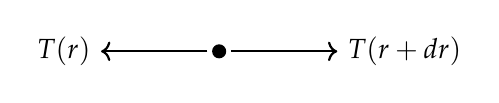
\begin{tikzpicture}[scale=1.5, thick]
        \draw[fill=black] (0,0) circle (0.05);
        \draw[->] (0.1, 0) -- (1, 0) node[right] {$T(r+dr)$};
        \draw[->] (-0.1, 0) -- (-1, 0) node[left] {$T(r)$};
    \end{tikzpicture}
    \end{center}
    
    \item What is the acceleration of this differential element of rope? (Write it as a vector.) \\
    \textcolor{blue}{\[ \vec{a} = -r\omega^2\hat{r} \]}
    What is its mass? (\textit{Hint:} Express the differential mass $dm$ in terms of $dr$ and quantities that are given in the statement of the problem.) \\
    \textcolor{blue}{For a uniform rope, $\frac{dm}{m} = \frac{dr}{\ell} \implies dm = \frac{m}{\ell}dr$.}
    
    \item Write Newton's 2nd Law for the differential element of rope, and convert it into a \textit{differential equation} for the tension. \\
    \textcolor{blue}{
    The net force is outward: $F_{\text{net, } r} = T(r+dr) - T(r) = dT$.
    Using $F = ma$:
    \[ dT = (dm)(-r\omega^2) = -\left(\frac{m}{\ell}dr\right)r\omega^2 \implies \frac{dT}{dr} = -\frac{m\omega^2}{\ell}r \]
    }
    
    \item Solve the differential equation by integrating over $r$. Think carefully about limits of integration. (For which value of $r$ do we already know $T$?) \\
    \textcolor{blue}{
    We know $T(\ell) = M\ell\omega^2$. We integrate from an arbitrary radius $r$ to $\ell$:
    \begin{align*}
        \int_{T(r)}^{T(\ell)} dT' &= \int_{r}^{\ell} -\frac{m\omega^2}{\ell} r' dr' \\
        T(\ell) - T(r) &= -\frac{m\omega^2}{\ell} \left[ \frac{1}{2}r'^2 \right]_{r}^{\ell} = -\frac{m\omega^2}{2\ell}(\ell^2 - r^2) \\
        T(r) &= T(\ell) + \frac{m\omega^2}{2\ell}(\ell^2 - r^2) = M\ell\omega^2 + \frac{1}{2}m\ell\omega^2\left(1 - \left(\frac{r}{\ell}\right)^2\right)
    \end{align*}
    }
    
    \item Now check limiting or special cases to compare your result with your physical reasoning, or to further \textit{develop} your physical reasoning. Can you think of \textit{four} cases to consider? \\
    \textcolor{blue}{
    1. $r = \ell \implies T(\ell) = M\ell\omega^2$ (matches our boundary condition). \\
    2. $m \to 0 \implies T(r) = M\ell\omega^2$ (massless rope has constant tension). \\
    3. $M \to 0 \implies T(r) = \frac{1}{2}m\ell\omega^2(1 - (r/\ell)^2)$ (tension due only to the rope's own mass). \\
    4. $\omega \to 0 \implies T(r) = 0$ (no rotation, no tension in outer space).
    }
    
    \item On your whiteboard, make a graph of $T(r)$ as a function of $r$ that illustrates some cases you may have considered in the previous subpart. Include a scale on each coordinate axis by indicating values that depend only on quantities given in the problem. \\
    \begin{center}
    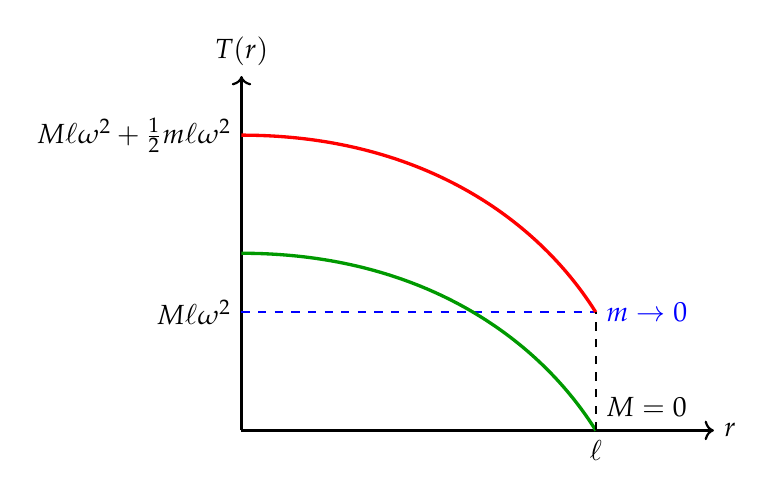
\begin{tikzpicture}[scale=1.5, thick]
        % Axes
        \draw[->] (0, 0) -- (0, 3) node[above] {$T(r)$};
        \draw[->] (0, 0) -- (4, 0) node[right] {$r$};
        
        % Constant tension
        \draw[dashed, blue] (0, 1) -- (3, 1) node[right] {$m \to 0$};
        \node[left] at (0, 1) {$M\ell\omega^2$};
        
        % Parabola
        \draw[red, very thick] (0, 2.5) .. controls (1.5, 2.5) and (2.5, 1.8) .. (3, 1);
        
        % M=0 parabola
        \draw[green!60!black, very thick] (0, 1.5) .. controls (1.5, 1.5) and (2.5, 0.8) .. (3, 0);
        \node[right] at (3, 0.2) {$M = 0$};
        
        % Labels
        \node[below] at (3, 0) {$\ell$};
        \draw[dashed] (3, 0) -- (3, 1);
        \node[left] at (0, 2.5) {$M\ell\omega^2 + \frac{1}{2}m\ell\omega^2$};
    \end{tikzpicture}
    \end{center}
    \textcolor{blue}{The tension is maximum at the center ($r=0$) and decreases quadratically to $M\ell\omega^2$ at the end ($r=\ell$).}
\end{enumerate}
\end{exercise}

\section*{Example \& Technique \#2: Viscous drag again --- Finding a particular solution}

In the previous example of viscous drag, adding gravity to the mix still resulted in a separable equation, but that isn't always the case. Here we will practice another technique: finding a \textit{particular} solution.

\begin{exercise}[Exercise 2]
Consider again the differential equation describing an object moving in only the vertical direction and experiencing viscous drag as well as gravity:
\[ m\frac{dv_y}{dt} = -Cv_y - mg \tag{1} \]

\begin{enumerate}[label=(\alph*)]
    \item Using physical reasoning about drag and falling objects, identify one very \textit{particular} solution to the equation of motion. (It doesn't have to be \textit{general} -- it could have very special initial conditions, for example.) Think about the behavior of the object after a long time. \\
    \textcolor{blue}{After a long time, the object reaches terminal velocity, where the acceleration is zero. Setting $dv_y/dt = 0$, we get $-Cv_y - mg = 0 \implies v_y = -mg/C$. So a particular solution is the constant function $v_y(t) = -mg/C$.}
    
    \item Now, \textbf{assume} that the true solution $v_y(t)$ is the `particular' solution you just found \textit{plus some other function} $u(t)$ that we need to find. Substitute this assumed form for $v_y(t)$ into the equation of motion for $v_y(t)$ to find the equation for $u(t)$, and then identify the solution.
    
    Assume $v_y(t) = u(t) + \left( \textcolor{blue}{-mg/C} \right)$; \quad then $\quad \frac{dv_y}{dt} = \textcolor{blue}{\frac{du}{dt}} \quad$ and 
    \[ v_y(0) = \textcolor{blue}{u(0) - \frac{mg}{C} = v_{y0} \implies u(0) = v_{y0} + \frac{mg}{C}} \]
    
    Substitute these expressions for $v_y(t)$ and $\frac{dv_y}{dt}$ into both sides of eq. 1 and solve for $u(t)$: \\
    \textcolor{blue}{
    \[ m\frac{du}{dt} = -C\left(u - \frac{mg}{C}\right) - mg = -Cu + mg - mg = -Cu \]
    This is the same differential equation we solved in Exercise 1! The solution is:
    \[ u(t) = u(0)e^{-\frac{C}{m}t} = \left(v_{y0} + \frac{mg}{C}\right)e^{-\frac{C}{m}t} \]
    }
    
    Finally, write an expression for $v_y(t)$: \\
    \textcolor{blue}{
    \[ v_y(t) = \left(v_{y0} + \frac{mg}{C}\right)e^{-\frac{C}{m}t} - \frac{mg}{C} \]
    }
\end{enumerate}
Check that your result for $v_y(t)$ is consistent with the expression we derived using Technique \#1 (separate and integrate).
\end{exercise}

\section*{Example \& Technique \#3: Linear restoring (`spring') force --- Guessing the form of a solution}

Consider an object at rest in a position of \textit{stable equilibrium}; for convenience, call that position $\vec{r} = 0$.

\textcolor{blue}{\textbf{Quick Exercise 3:}}
\begin{enumerate}[label=(\alph*)]
    \item How is a position of equilibrium defined? \\
    \textcolor{blue}{$\vec{F}_{\text{net}} = 0$, $\vec{v} = 0$.}
    \item How is a position of \textit{stable} equilibrium defined? \\
    \textcolor{blue}{A point where small displacements result in a restoring force pointing back towards the equilibrium point.}
    \item What other kinds of equilibrium points are there? \\
    \textcolor{blue}{Unstable equilibrium (forces push away from the point) and saddle points (stable in one direction, unstable in another).}
\end{enumerate}

For now, let's consider motion in only one dimension, $x$. (The higher dimensional cases have more possibilities.) For $x = 0$ to be a point of stable equilibrium, $F_x$ must be negative for small positive values of $x$ and positive for small negative values of $x$. In fact, for small enough $x$ we can just write the leading term in the Taylor series expansion:
\[ F_x = -kx. \]

\textcolor{blue}{\textbf{Make a sketch of $F_x$ versus $x$.}}
\begin{center}
\begin{tikzpicture}[scale=1.5, thick]
    \draw[->] (-2, 0) -- (2, 0) node[right] {$x$};
    \draw[->] (0, -2) -- (0, 2) node[above] {$F_x$};
    \draw[blue, very thick] (-1.5, 1.5) -- (1.5, -1.5) node[right] {$F_x = -kx$};
\end{tikzpicture}
\end{center}

The equation $F_x = -kx$ is known as Hooke's Law when describing the restoring force due to a spring -- but it's not a fundamental ``law''; it's just a good approximation for springs, for small enough displacements. However, it is very useful when describing small displacements from any stable equilibrium (along one direction).

\begin{exercise}[Exercise 4]
Consider a mass acted on by a linear restoring force (a.k.a. attached to a spring) in the $x$ direction: $F_x = -kx$.
\begin{enumerate}[label=(\alph*)]
    \item Describe the motion of the mass. What \textit{simple} function(s) might you expect to describe the motion of the mass? Write a \textit{dimensionally consistent} \textbf{guess} for $x(t)$. It's OK to introduce unknown dimensionful constants\dots \\
    \textcolor{blue}{We expect oscillatory motion. A good guess is a sine or cosine function:
    \[ x(t) = A\sin(\omega t) \]
    where $A$ is the amplitude and $\omega$ is the angular frequency.}
    
    \item Write the equation of motion for this system, and plug in your guess, determining any unknown constants that you can.
    \[ m\frac{d^2x}{dt^2} = F_x \implies \textcolor{blue}{m\frac{d^2}{dt^2}\left[ A\sin(\omega t) \right] = -k\left[ A\sin(\omega t) \right]} \]
    \textcolor{blue}{
    \begin{align*}
        m\frac{d}{dt}\left[ A\omega\cos(\omega t) \right] &= -kA\sin(\omega t) \\
        -mA\omega^2\sin(\omega t) &= -kA\sin(\omega t) \\
        m\omega^2 &= k \implies \omega = \sqrt{\frac{k}{m}}
    \end{align*}
    }
    
    \item Since we didn't \textit{integrate} the 2nd-order differential equation (and in general we can't, unless we can write it as a first-order differential equation), we can't account for our initial conditions by using definite integrals. Instead we must incorporate the initial conditions by using them to solve for unknown coefficients in our solutions. Since we can always specify two initial conditions (position and velocity), we need \textit{two} arbitrary coefficients for a general solution. If your initial guess wasn't general enough, try making a more general guess. Then eliminate the arbitrary coefficients in favor of $x_0 \equiv x(0)$ and $v_0 \equiv v_x(0)$. \\
    \textcolor{blue}{
    General guess: $x(t) = A\sin(\omega t) + B\cos(\omega t)$, with $\omega = \sqrt{k/m}$.
    \begin{align*}
        x(0) &= B \implies B = x_0 \\
        v_x(t) &= A\omega\cos(\omega t) - B\omega\sin(\omega t) \\
        v_x(0) &= A\omega \implies A = \frac{v_0}{\omega}
    \end{align*}
    So the solution in terms of initial conditions is:
    \begin{align*}
        x(t) &= \frac{v_0}{\omega}\sin(\omega t) + x_0\cos(\omega t) \\
        v_x(t) &= v_0\cos(\omega t) - x_0\omega\sin(\omega t)
    \end{align*}
    }
    
    \item Finally, suppose we had \textit{no idea} what functions to guess. Let's solve this equation somewhat differently. One of the most common functions to appear in the solutions of differential equations is the \textit{exponential}. Even though it may seem totally unphysical to this situation, try solving the differential equation (and applying the initial conditions) by assuming a function of the form $x(t) = Ce^{\alpha t}$. \\
    $[$Introduce $\omega \equiv \sqrt{k/m}$ at an appropriate point.$]$ \\
    Here is a reminder of the differential equation to solve: $m\frac{d^2x}{dt^2} = -kx$. \\
    \textcolor{blue}{
    Substitute $x(t) = Ce^{\alpha t}$:
    \begin{align*}
        m\frac{d^2}{dt^2}\left( Ce^{\alpha t} \right) &= -k\left( Ce^{\alpha t} \right) \\
        mC\alpha^2 e^{\alpha t} &= -kCe^{\alpha t} \\
        m\alpha^2 &= -k \\
        \alpha^2 &= -\frac{k}{m} \implies \alpha = \pm i\sqrt{\frac{k}{m}} = \pm i\omega
    \end{align*}
    Since there are two possible values for $\alpha$, the general solution is a linear combination of both:
    \[ x(t) = C_1 e^{i\omega t} + C_2 e^{-i\omega t} \]
    }
    And plugging in initial conditions\dots \\
    \textcolor{blue}{
    \begin{align*}
        x(0) &= C_1 + C_2 = x_0 \\
        v_x(t) &= i\omega C_1 e^{i\omega t} - i\omega C_2 e^{-i\omega t} \\
        v_x(0) &= i\omega(C_1 - C_2) = v_0 \implies C_1 - C_2 = \frac{v_0}{i\omega} = -i\frac{v_0}{\omega}
    \end{align*}
    Solving for $C_1$ and $C_2$:
    \[ C_1 = \frac{1}{2}\left( x_0 - i\frac{v_0}{\omega} \right), \quad C_2 = \frac{1}{2}\left( x_0 + i\frac{v_0}{\omega} \right) \]
    }
    
    \item Discuss: How are these two different approaches equivalent? \\
    \textit{Hint:} You may want to recall ``Euler's formula'' (if you have encountered it in the past\footnote{See one of the problems of Problem Set 7 for a demonstration of Euler's formula using Taylor's series for the exponential and trig functions.}):
    \[ e^{i\omega t} = \cos\omega t + i\sin\omega t. \]
    \textcolor{blue}{
    Substitute Euler's formula into the complex exponential solution:
    \begin{align*}
        x(t) &= C_1(\cos\omega t + i\sin\omega t) + C_2(\cos\omega t - i\sin\omega t) \\
             &= (C_1 + C_2)\cos\omega t + i(C_1 - C_2)\sin\omega t
    \end{align*}
    Using the relations for $C_1$ and $C_2$ found above:
    \begin{align*}
        C_1 + C_2 &= x_0 \\
        i(C_1 - C_2) &= i\left( -i\frac{v_0}{\omega} \right) = \frac{v_0}{\omega}
    \end{align*}
    This perfectly reproduces our previous result:
    \[ x(t) = x_0\cos\omega t + \frac{v_0}{\omega}\sin\omega t \]
    }
\end{enumerate}
\end{exercise}

% ==================== LECTURE 20 ====================
\chapter{Newton's Laws \& Momentum of a System}

Read Chapter 4 in Kleppner \& Kolenkow: Momentum.

For an object that can be treated as a single point-like ``particle'' of mass $m$ with position vector $\vec{r}(t)$ in an inertial frame, we can write Newton's 2nd Law as $\vec{F} = m\vec{a} \equiv m\frac{d\vec{v}}{dt} \equiv m\frac{d^2\vec{r}}{dt^2}$, where $\vec{F}$ is the net force acting on the particle.

We can also write the 2nd Law in the form that Newton wrote it,
\[ \vec{F} = \frac{d\vec{p}}{dt}, \tag{1} \]
where $\vec{p} = m\vec{v}$ is called the \textit{momentum} of the particle.

\textcolor{blue}{\textbf{Quick Question:} Under what condition(s) is Newton's form of the 2nd Law the same as $\vec{F} = m\vec{a}$?} \\
\textcolor{blue}{
\[ \vec{F} = \frac{d\vec{p}}{dt} = \frac{d}{dt}(m\vec{v}) = m\frac{d\vec{v}}{dt} + \frac{dm}{dt}\vec{v} \]
They are the same only if the mass is constant ($\frac{dm}{dt} = 0$).
}

\begin{center}
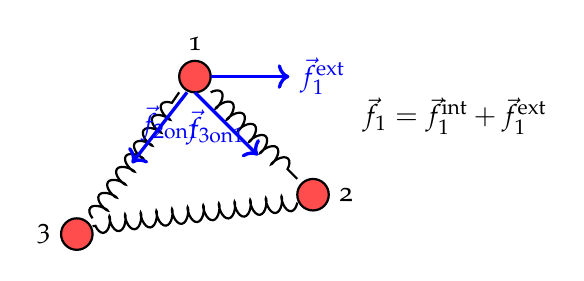
\begin{tikzpicture}[scale=1, thick]
    % Particles
    \draw[fill=red!70] (0, 1.5) circle (0.2) node[above=2mm] {1};
    \draw[fill=red!70] (1.5, 0) circle (0.2) node[right=2mm] {2};
    \draw[fill=red!70] (-1.5, -0.5) circle (0.2) node[left=2mm] {3};
    
    % Springs
    \draw[decorate, decoration={coil, aspect=0.4, segment length=2mm, amplitude=1mm}] (0.2, 1.3) -- (1.3, 0.2);
    \draw[decorate, decoration={coil, aspect=0.4, segment length=2mm, amplitude=1mm}] (1.3, -0.1) -- (-1.3, -0.4);
    \draw[decorate, decoration={coil, aspect=0.4, segment length=2mm, amplitude=1mm}] (-1.3, -0.3) -- (-0.2, 1.3);
    
    % Forces
    \draw[->, blue, very thick] (0.2, 1.5) -- (1.2, 1.5) node[right] {$\vec{f}_{1}^{\text{ext}}$};
    \draw[->, blue, very thick] (0, 1.3) -- (0.8, 0.5) node[midway, left=2mm] {$\vec{f}_{2\text{on}1}$};
    \draw[->, blue, very thick] (-0.1, 1.3) -- (-0.8, 0.4) node[midway, right=2mm] {$\vec{f}_{3\text{on}1}$};
    
    % Equation node
    \node[right] at (2, 1) {$\vec{f}_1 = \vec{f}_1^{\text{int}} + \vec{f}_1^{\text{ext}}$};
\end{tikzpicture}
\end{center}

Consider a \textit{system} of $N$ (\textbf{possibly interacting}) particles; the $i$th particle has mass $m_i$, velocity $\vec{v}_i$, and momentum $\vec{p}_i = m_i\vec{v}_i$. Define $\vec{P}$ to be the \textit{total} momentum of the system:
\[ \vec{P} = \sum_i^N \vec{p}_i. \]

\begin{exercise}[Exercise 1]
In this exercise, you will show that Newton's Laws lead to this result for the system:
\[ \vec{F}_{\text{ext}} = \frac{d\vec{P}}{dt}, \tag{2} \]
where $\vec{F}_{\text{ext}}$ is the net \textit{external} force acting on the system of particles. Follow the steps outlined below and identify where any of Newton's Laws are being invoked along the way.

First break the forces acting on particle $i$ into two parts:
\[ \vec{f}_i = \vec{f}_i^{\text{int}} + \vec{f}_i^{\text{ext}}, \]
where $\vec{f}_i^{\text{int}}$ is the total \textit{internal} force acting on $i$, due to all other particles in the system, and $\vec{f}_i^{\text{ext}}$ is the total \textit{external} force acting on $i$, due to sources outside the system.
\begin{enumerate}[label=(\alph*)]
    \item Write $\vec{f}_i^{\text{int}} = \sum_j (\text{what?})$? \\
    \textcolor{blue}{\[ \vec{f}_i^{\text{int}} = \sum_{j \neq i}^N \vec{f}_{j\text{ on }i} \]}
    \item Write Newton's 2nd Law in the form of equation 1 applied to only particle $i$, with $\vec{f}_i = \vec{f}_i^{\text{int}} + \vec{f}_i^{\text{ext}}$. \\
    \textcolor{blue}{\[ \vec{f}_i^{\text{int}} + \vec{f}_i^{\text{ext}} = \frac{d\vec{p}_i}{dt} \]}
\end{enumerate}
\end{exercise}

\begin{enumerate}[label=(\alph*), resume]
    \item Now sum the two sides of the equation $\vec{f}_i^{\text{int}} + \vec{f}_i^{\text{ext}} = \frac{d\vec{p}_i}{dt}$ over \textit{all} particles in the system and then consider each of the three sums carefully to arrive at the result in equation 2. (Use the result from (a) above.) \\
    \textcolor{blue}{
    \begin{align*}
        \sum_{i=1}^N \left( \vec{f}_i^{\text{int}} + \vec{f}_i^{\text{ext}} \right) &= \sum_{i=1}^N \frac{d\vec{p}_i}{dt} \\
        \underbrace{\sum_{i=1}^N \sum_{j \neq i} \vec{f}_{j\text{ on }i}}_{\text{Newton's 3rd Law pairs cancel}} + \sum_{i=1}^N \vec{f}_i^{\text{ext}} &= \frac{d}{dt} \sum_{i=1}^N \vec{p}_i \\
        0 + \vec{F}_{\text{ext}} &= \frac{d\vec{P}}{dt}
    \end{align*}
    }
    
    \item On which of Newton's Laws does the result (eq. 2) depend? \\
    \textcolor{blue}{Newton's Third Law (to cancel the internal forces) and Newton's Second Law.}
\end{enumerate}

\begin{exercise}[Exercise 2]
Which of the following statements about the result $\vec{F}_{\text{ext}} = \frac{d\vec{P}}{dt}$ are true?
\begin{enumerate}
    \item $\vec{F}_{\text{ext}}$ could be a \textit{single} type of external force acting on a \textit{single} particle in the system. \textbf{\textcolor{blue}{True}} or False?
    \item $\vec{F}_{\text{ext}}$ could be due to \textit{many} types of external forces acting on a \textit{single} particle in the system. \textbf{\textcolor{blue}{True}} or False?
    \item $\vec{F}_{\text{ext}}$ could be a \textit{single} type of external force acting on \textit{many} particles in the system. \textbf{\textcolor{blue}{True}} or False?
    \item $\vec{F}_{\text{ext}}$ could be due to \textit{many} types of external forces acting on \textit{many} particles in the system. \textbf{\textcolor{blue}{True}} or False?
    \item The result can be applied to a `system' composed of a nonrigid extended object, such as two masses stuck to opposite ends of an elastic cord. \textbf{\textcolor{blue}{True}} or False?
    \item The result can be applied to a system composed of two objects that collide and stick together. \textbf{\textcolor{blue}{True}} or False? \textcolor{blue}{(Heat is generated, but momentum is still governed by external forces.)}
    \item The result can be applied to a system composed of a single object that explodes into many objects. \textbf{\textcolor{blue}{True}} or False?
    \item The result can be applied to a system of many particles with \textit{no} internal interactions. \textbf{\textcolor{blue}{True}} or False?
    \item The result can be applied to a system with internal dissipative forces, like friction. \textbf{\textcolor{blue}{True}} or False? \textcolor{blue}{(Depends -- if heat is transferred to air outside the system, we must account for it. If the whole system is isolated, it's still true.)}
\end{enumerate}
\end{exercise}

\section*{Mass-weighted position (a.k.a. center-of-mass position)}

Consider a system of $N$ point particles at time $t$. Particle $i$ has mass $m_i$ and is located at position $\vec{r}_i(t)$.

\begin{center}
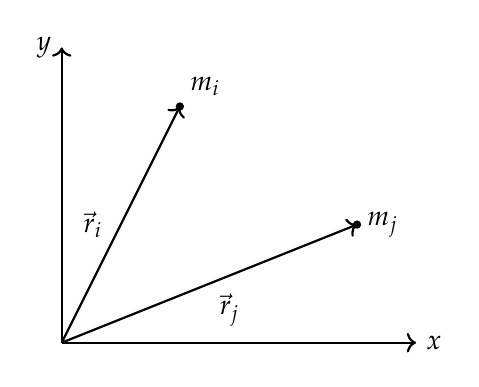
\begin{tikzpicture}[scale=1.5, thick]
    \draw[->] (0,0) -- (3,0) node[right] {$x$};
    \draw[->] (0,0) -- (0,2.5) node[left] {$y$};
    
    \draw[->] (0,0) -- (1, 2) node[above right] {$m_i$} node[midway, left=1mm] {$\vec{r}_i$};
    \draw[->] (0,0) -- (2.5, 1) node[right] {$m_j$} node[midway, below right] {$\vec{r}_j$};
    
    \fill (1,2) circle (1pt);
    \fill (2.5,1) circle (1pt);
\end{tikzpicture}
\end{center}

Define the vector $\vec{R}(t)$ to be the ``mass-weighted position'' of the system of particles:
\[ \vec{R}(t) \equiv \frac{1}{M}\sum_{i=1}^N m_i\vec{r}_i(t), \tag{3} \]
where $M$ is defined to be the total mass of the system:
\[ M \equiv \sum_i m_i. \]

\begin{exercise}[Exercise 3]
Differentiate the above expression for $\vec{R}$ twice with respect to time to show that $M\frac{d^2\vec{R}}{dt^2} = \frac{d\vec{P}}{dt}$. \\
\textcolor{blue}{
\begin{align*}
    M\vec{R} &= \sum_{i=1}^N m_i\vec{r}_i(t) \\
    M\frac{d\vec{R}}{dt} &= \frac{d}{dt}\sum_{i=1}^N m_i\vec{r}_i(t) = \sum_{i=1}^N m_i\vec{v}_i(t) \quad \text{\footnotesize{(Take one derivative inside summation.)}} \\
    M\frac{d^2\vec{R}}{dt^2} &= \frac{d}{dt}\sum_{i=1}^N m_i\vec{v}_i(t) = \sum_{i=1}^N m_i\vec{a}_i(t) \\
    &= \sum_{i=1}^N \vec{F}_i^{\text{net}} = \sum_{i=1}^N \vec{F}_i^{\text{ext}} \quad \text{\footnotesize{(Internal forces cancel)}} \\
    &= \vec{F}_{\text{ext}} = \frac{d\vec{P}}{dt} \quad \ddot{\smile}
\end{align*}
}
\end{exercise}

Therefore, we now have two equivalent statements of Newton's Laws applied to a system of particles:
\[ \vec{F}_{\text{ext}} = \frac{d\vec{P}}{dt} \iff \vec{F}_{\text{ext}} = M\frac{d^2\vec{R}}{dt^2} \]

The vector $\vec{R}$ is the position vector for a special point called the \textit{center of mass} of the system of particles.

\begin{exercise}[Exercise 4]
Describe the equation $\vec{F}_{\text{ext}} = M\frac{d^2\vec{R}}{dt^2}$ in words -- including why it is so powerful. \\
\textcolor{blue}{The center of mass of a system of particles moves exactly as if it were a single particle of mass $M$ acted upon by the net external force $\vec{F}_{\text{ext}}$. It is powerful because it allows us to treat complex, extended, or multi-particle systems as simple point masses when calculating their overall translational motion, completely ignoring internal forces!}
\end{exercise}

\textbf{Summary:}

For a point-like particle, Newton's 2nd Law $\implies$
\[ \vec{F} = m\frac{d^2\vec{r}}{dt^2} \iff \vec{F} = \frac{d\vec{p}}{dt} \tag{4} \]

For a \textit{system} of particles, Newton's 2nd \textit{and 3rd} Laws $\implies$
\[ \vec{F}_{\text{ext}} = M\frac{d^2\vec{R}}{dt^2} \iff \vec{F}_{\text{ext}} = \frac{d\vec{P}}{dt} \tag{5} \]

Similar to Exercise 3, we can differentiate $\vec{R}$ once and use the definitions of $\vec{P}$ and $M$ to also show that
\[ \vec{P} = M\vec{V}, \text{ where } \vec{V} \equiv \frac{d\vec{R}}{dt}. \quad \text{\footnotesize{\textcolor{blue}{Show this on your own, for practice.}}} \]

\textcolor{blue}{\textbf{Question:} Is $\vec{V} = \sum_i \vec{v}_i$, where $\vec{v}_i = d\vec{r}_i/dt$?} \\
\textcolor{blue}{No, $\vec{V} = \frac{1}{M}\sum_i m_i\vec{v}_i$. It is the mass-weighted average of the velocities, not the simple sum.}

\textbf{Useful Note:} To find the center of mass of a system of multiple subsystems, we just find the mass $M_j$ and center of mass location $\vec{R}_j$ of each subsystem, and then combine them like point particles with mass $M_j$ located at position $\vec{R}_j$.

\begin{center}
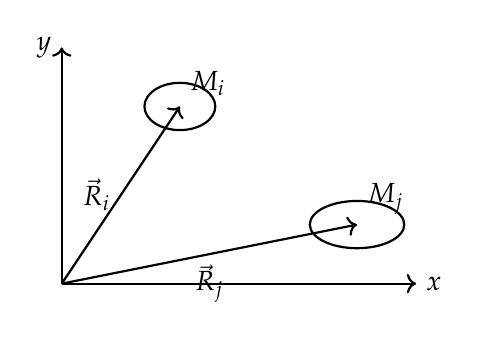
\begin{tikzpicture}[scale=1.5, thick]
    \draw[->] (0,0) -- (3,0) node[right] {$x$};
    \draw[->] (0,0) -- (0,2) node[left] {$y$};
    
    \draw[->] (0,0) -- (1, 1.5) node[midway, left] {$\vec{R}_i$};
    \draw[->] (0,0) -- (2.5, 0.5) node[midway, below] {$\vec{R}_j$};
    
    \draw (1,1.5) ellipse (0.3 and 0.2) node[above right] {$M_i$};
    \draw (2.5,0.5) ellipse (0.4 and 0.2) node[above right] {$M_j$};
\end{tikzpicture}
\end{center}

\subsection*{Conservation of Momentum}

An important consequence of the above formulation of Newton's Laws is that \textbf{if} $\vec{F}_{\text{ext}} = 0$ -- i.e., there is no \textit{net} external force acting on the system or, in other words, the system is \textit{isolated} -- then the total momentum of the system is a conserved quantity:
\[ \frac{d\vec{P}}{dt} = 0, \text{ or equivalently } \frac{d^2\vec{R}}{dt^2} = \frac{d\vec{V}}{dt} = 0. \]
$\implies$ Independent of how many \textit{internal} forces may be at play,
\begin{itemize}
    \item the total momentum of an isolated system is conserved, and
    \item the location of the center of mass moves with constant velocity $\vec{V} = d\vec{R}/dt$.
\end{itemize}
These results are general and apply equally to an ``isolated'' ($\vec{F}_{\text{ext}} = 0$) collection of individual objects (balls colliding on a frictionless billiard table), to an isolated extended object, and even to an isolated exploding object -- because in each case all the forces are \textit{internal}!

\section*{Center of Mass Coordinates}

The ``center-of-mass coordinate system'' is defined as a (possibly moving) set of coordinate axes for which \textbf{the origin is located at the position of the center of mass} (CM). Let's use primed coordinates ($x'$ and $y'$) to designate the CM coordinate system.

\begin{center}
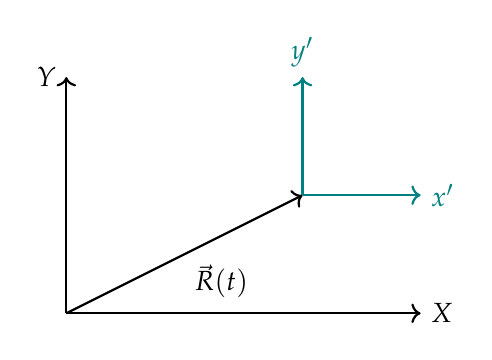
\begin{tikzpicture}[scale=1.5, thick]
    \draw[->] (0,0) -- (3,0) node[right] {$X$};
    \draw[->] (0,0) -- (0,2) node[left] {$Y$};
    
    \draw[->] (0,0) -- (2, 1) node[midway, below right] {$\vec{R}(t)$};
    
    \draw[->, color=teal] (2,1) -- (3, 1) node[right] {$x'$};
    \draw[->, color=teal] (2,1) -- (2, 2) node[above] {$y'$};
\end{tikzpicture}
\end{center}

\begin{exercise}[Exercise 5]
Does the CM coordinate system necessarily define an inertial frame of reference? \\
\textcolor{blue}{Yes, \textbf{if} there is no net external force ($\vec{F}_{\text{ext}} = 0$). \\
No, \textbf{if} there is a net external force, the CM accelerates, making the frame non-inertial.}
\end{exercise}

\begin{exercise}[Exercise 6]
Show that in the CM system the total momentum $\vec{P}'$ is 0. \\
\textit{Hint:} In the CM coordinate system, what is the position $\vec{R}'$ of the CM? Use this information along with the \textit{definition} of the CM position (eq. 3) and differentiate. \\
\textcolor{blue}{
By definition, the origin of the CM coordinate system is the CM itself. Therefore, the position of the CM in the primed coordinates is always zero: $\vec{R}' = \vec{0}$.
\[ \vec{V}' = \frac{d\vec{R}'}{dt} = \vec{0} \implies \vec{P}' = M\vec{V}' = \vec{0} \text{ (since } M \neq 0). \]
Alternatively, using the sum definition:
\[ \vec{R}' = \frac{1}{M}\sum_{i=1}^N m_i\vec{r}_i' = \vec{0} \implies \sum_{i=1}^N m_i\vec{v}_i' = \vec{0} \implies \vec{P}' = \vec{0}. \]
}
\end{exercise}

\textbf{Summary:} In the CM coordinate system, the total momentum $\vec{P}'$ is 0 -- as well as being conserved since it is \textit{always} 0 in the CM coordinate system!

Therefore, for a system of two masses, for example, $m_1\vec{r}_1' + m_2\vec{r}_2' = 0$ and $\vec{p}_1' + \vec{p}_2' = 0$. \\
$\implies$ The mass-weighted position vectors of the two particles in the CM coordinate system are related by the simple expression $m_1\vec{r}_1' = -m_2\vec{r}_2'$ and their momentum vectors are related by $\vec{p}_1' = -\vec{p}_2'$.

For an \textit{isolated} system (no net external force acting on the system), the CM location will move with constant velocity in an inertial reference frame; in that case, the CM coordinate system itself defines an inertial reference frame.

If the system is not isolated, then the position of the origin of the CM coordinate system will satisfy equation 5 above, repeated here:
\[ \vec{F}_{\text{ext}} = M\frac{d^2\vec{R}}{dt^2} \iff \vec{F}_{\text{ext}} = \frac{d\vec{P}}{dt} \tag{6} \]
In that case, the CM coordinate system does not define an inertial reference frame.

\textcolor{blue}{\textbf{Video Demonstration:} Watch this MIT video demonstration of the motion of the CM of two interacting objects: \url{https://www.youtube.com/watch?v=amfw2nABke4} \\
Which location corresponds to $\vec{R}$? Is $\vec{P}$ constant? In which reference frame is $\vec{P}' = 0$ and $\vec{p}_1' = -\vec{p}_2'$?}

% ==================== LECTURE 21 ====================
\chapter{CM Location; Rocket Science!}

\section*{Finding the Center-of-Mass Location for an Extended Object}

\begin{exercise}[Exercise 1]
To calculate the CM location for an extended object, imagine dividing the object into $N$ mass elements $m_i$ and letting $N$ approach infinity so that the mass of each infinitesimal element approaches zero.
\begin{enumerate}[label=(\alph*)]
    \item Write the location of the CM as an integral: \\
    \textcolor{blue}{\[ \vec{R} = \lim_{N\to\infty} \frac{1}{M}\sum_{i=1}^N m_i\vec{r}_i = \frac{1}{M}\int_{\text{vol}} \vec{r} \, dm \]}
    \item Write the expression for just the $X$ coordinate of the CM location: \\
    \textcolor{blue}{\[ X = \frac{1}{M}\int_{\text{vol}} x \, dm \]}
    \item Suppose you are given the density $\rho(\vec{r})$ at each point $\vec{r}$ in the extended object. Write an expression for the CM location as an integral involving $\rho(\vec{r})$. (Think about how to express $dm$ in terms of $\rho(\vec{r})$ and a differential element -- which one?) \\
    \textcolor{blue}{
    \[ \rho(\vec{r}) = \frac{dm}{dV} \implies dm = \rho(\vec{r})\,dV \]
    \[ \vec{R} = \frac{1}{M}\int_{\text{vol}} \vec{r}\rho(\vec{r})\,dV \]
    }
\end{enumerate}
\end{exercise}

In problems, you may encounter mass density described as volume density, surface density, or linear density. Here are the Greek letters typically used for each quantity, along with the dimensions of each.
\begin{itemize}
    \item $\rho$ (rho), volume density (mass per unit volume): $[\rho] = \mathbf{M}/\mathbf{L}^3$.
    \item $\sigma$ (sigma), surface density (mass per unit area): $[\sigma] = \mathbf{M}/\mathbf{L}^2$.
    \item $\lambda$ (lambda), linear density (mass per unit length): $[\lambda] = \mathbf{M}/\mathbf{L}$.
\end{itemize}

\vspace{0.5em}\hrule\vspace{0.5em}

We are now ready to apply these new formulations of Newton's Laws, and the useful definition and properties of the CM location, in a couple of activities.

We will use the equation developed above to find the position of the center of mass of an extended object:
\[ \vec{R} = \frac{1}{M}\int_{\text{Vol}} \vec{r}\,dm. \quad \text{\footnotesize{The integral is over the entire volume.}} \]

\textcolor{blue}{\textbf{Quick Exercise 2:} Does the position of the center of mass of an extended object depend on the \textit{total} mass of the object?} \\
Answer: Yes or \textbf{\textcolor{blue}{No}}?

Although the CM location does not depend on the total mass $M$, it can be useful to introduce $M$ when finding the position of the center of mass.

\begin{exercise}[Exercise 3]
In this exercise, we will find the center-of-mass (CM) location of a semi-circular strip of radius $R$, illustrated below. Assume the density and thickness are uniform, and that the radial extent of the strip is much less than the radius.
\begin{enumerate}[label=(\alph*)]
    \item What is the $X$ coordinate of the CM location? Why? \\
    \textcolor{blue}{$X=0$, due to symmetry across the $Y$-axis.}
    
    \item Find the $Y$ coordinate of the CM location. \\
    \textit{Hint:} Once you write the expression for $Y$ in cartesian coordinates, try expressing each part of the integral in more suitable coordinates. What would those coordinates be? \\
    \begin{center}
    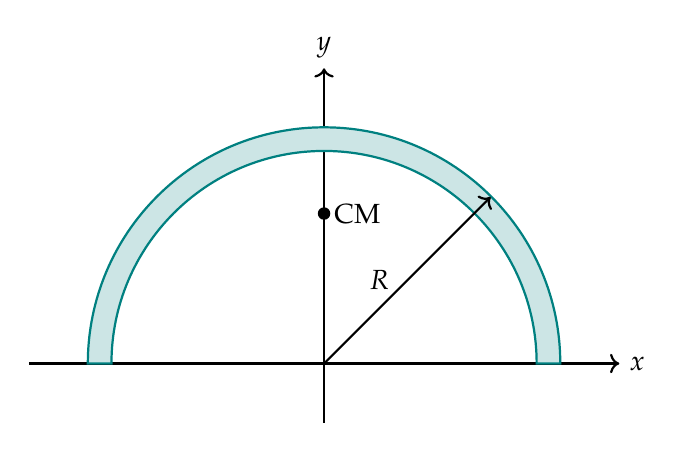
\begin{tikzpicture}[scale=1.5, thick]
        \draw[->] (-2.5,0) -- (2.5,0) node[right] {$x$};
        \draw[->] (0,-0.5) -- (0,2.5) node[above] {$y$};
        
        \draw[color=teal, fill=teal!20] (2,0) arc (0:180:2) -- (-1.8,0) arc (180:0:1.8) -- cycle;
        
        \fill (0,1.27) circle (1.5pt) node[right] {CM};
        \draw[->] (0,0) -- (1.41, 1.41) node[midway, left=1mm] {$R$};
    \end{tikzpicture}
    \end{center}
    \textcolor{blue}{
    The arc length element is $R\,d\theta$. The total length is $\pi R$, so $dm = \frac{M}{\pi R}(R\,d\theta) = \frac{M}{\pi}d\theta$.
    \begin{align*}
        Y &= \frac{1}{M}\int y\,dm \\
        Y_{CM} &= \frac{1}{M}\int_0^\pi (R\sin\theta)\left(\frac{M}{\pi}d\theta\right) \\
        &= \frac{R}{\pi}\int_0^\pi \sin\theta\,d\theta \\
        &= \frac{-R\cos\theta}{\pi} \Big|_0^\pi = \frac{-R(-1) - (-R(1))}{\pi} = \frac{2R}{\pi}
    \end{align*}
    }
    
    \item Indicate the location of the CM on the diagram. \textcolor{blue}{(Done above, plotted at $y = 2R/\pi \approx 0.64R$).}
\end{enumerate}
\end{exercise}

\section*{Rocket Science!}

Consider an isolated rocket system, illustrated in the figure below.
\begin{itemize}
    \item During a time $\Delta t$, the rocket engine exerts an \textit{internal} force that accelerates some of the fuel, of mass $\Delta m$, expelling it from the rocket with exhaust velocity $\vec{u}$ -- \textit{relative to the rocket}.
    \item By Newton's 3rd Law, there is an equal and opposite (internal) force on the rocket, that propels the rocket in the direction opposite to the fuel.
    \item The mass of the rocket\footnote{Note that when we refer to the ``mass of the rocket'', $M(t)$, we mean the mass of the rocket assembly plus the fuel remaining in the rocket.}, $M(t)$, is changing with time.
\end{itemize}

\begin{center}
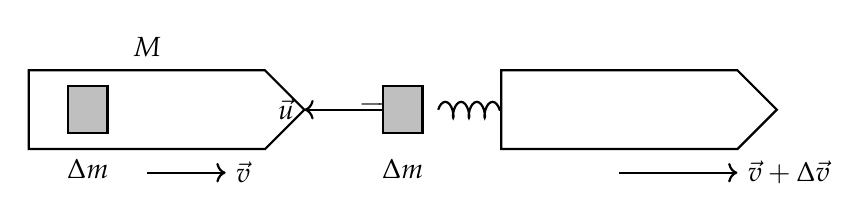
\begin{tikzpicture}[scale=1, thick]
    % Time t
    \draw (0,0) -- (3,0) -- (3.5, 0.5) -- (3,1) -- (0,1) -- cycle;
    \node at (1.5, 1.3) {$M$};
    \draw[->] (1.5, -0.3) -- (2.5, -0.3) node[right] {$\vec{v}$};
    
    % Fuel inside
    \draw[fill=gray!50] (0.5, 0.2) rectangle (1, 0.8);
    \node[below] at (0.75, 0) {$\Delta m$};
    
    \node at (4.5, 0.5) {$\implies$};
    
    % Time t + dt
    \begin{scope}[shift={(6,0)}]
        \draw (0,0) -- (3,0) -- (3.5, 0.5) -- (3,1) -- (0,1) -- cycle;
        \draw[->] (1.5, -0.3) -- (3, -0.3) node[right] {$\vec{v} + \Delta\vec{v}$};
        
        % Fuel expelled
        \draw[fill=gray!50] (-1.5, 0.2) rectangle (-1, 0.8);
        \draw[->] (-1.5, 0.5) -- (-2.5, 0.5) node[left] {$\vec{u}$};
        \node[below] at (-1.25, 0) {$\Delta m$};
        
        % Exhaust plume
        \draw[decorate, decoration={coil, aspect=0.4, segment length=2mm, amplitude=1mm}] (-0.8, 0.5) -- (0, 0.5);
    \end{scope}
\end{tikzpicture}
\end{center}

In the exercise below, you will determine the ``rocket equation'' -- a differential equation that relates the rate of change of the velocity of the rocket ($d\vec{v}/dt$) to the rate of change of the mass of the rocket ($dM/dt$) and the (relative) exhaust velocity $\vec{u}$.

For the initial part of the analysis, assume the rocket is coasting in free space with velocity $\vec{v}$ at time $t$, before expelling the bit of fuel.
\begin{itemize}
    \item Let the initial mass of the rocket at time $t$ be $M + \Delta m$.
    \item At time $t$, a thruster engine fires and expels mass $\Delta m$ with relative velocity $\vec{u}$ in the time interval $\Delta t$.
    \item Assume the velocity of the rocket at time $t + \Delta t$ is $\vec{v} + \Delta\vec{v}$.
\end{itemize}

Do not make any assumptions about the relative directions of $\vec{v}$, $\vec{u}$, or $\Delta\vec{v}$. By using vector notation throughout, you can solve the problem for the most general case of any relative directions!

\begin{exercise}[Exercise 4]
Work through the following steps on your whiteboard to find the rocket equation.
\begin{enumerate}[label=(\alph*)]
    \item Make sketches of the system at time $t$ and at time $t + \Delta t$. Carefully label all masses and all velocities. Be sure that all velocities are measured in the \textit{same} inertial frame. \\
    \textcolor{blue}{In the fixed inertial frame, the fuel is expelled with velocity $\vec{u} + \vec{v}$.}
    
    \item Write expressions for the total momentum $\vec{P}$ of the system at time $t$ and at time $t + \Delta t$. Then write an expression for the \textit{change} in total momentum, $\Delta\vec{P}$, in time $\Delta t$. \\
    \textcolor{blue}{
    \begin{align*}
        \vec{P}(t) &= (M + \Delta m)\vec{v} \\
        \vec{P}(t+\Delta t) &= \Delta m(\vec{u} + \vec{v}) + M(\vec{v} + \Delta\vec{v}) \\
        \Delta\vec{P} &= \vec{P}(t+\Delta t) - \vec{P}(t) \\
        &= \Delta m\vec{u} + \Delta m\vec{v} + M\vec{v} + M\Delta\vec{v} - M\vec{v} - \Delta m\vec{v} \\
        &= \Delta m\vec{u} + M\Delta\vec{v}
    \end{align*}
    }
    
    \item Find an expression for $d\vec{P}/dt$ by dividing $\Delta\vec{P}$ by $\Delta t$ and taking the limit as $\Delta t \to 0$ so that we are now considering the \textit{instantaneous} rate of change in various quantities at time $t$: \\
    \textcolor{blue}{
    \[ \frac{d\vec{P}(t)}{dt} = \lim_{\Delta t\to 0}\left( \frac{\Delta m\,\vec{u} + M\Delta\vec{v}}{\Delta t} \right) = \frac{dm}{dt}\vec{u} + M\frac{d\vec{v}}{dt} \]
    Use the relationship between $\frac{dm}{dt}$ (rate of fuel expelled) and $\frac{dM}{dt}$ (rate of change of rocket's mass) to eliminate $m$:
    Since the fuel expelled is the mass lost by the rocket, $\frac{dm}{dt} = -\frac{dM}{dt}$.
    \[ \frac{d\vec{P}(t)}{dt} = - \frac{dM}{dt}\vec{u} + M\frac{d\vec{v}}{dt} = M\frac{d\vec{v}}{dt} - \vec{u}\frac{dM}{dt} \]
    }
\end{enumerate}
\end{exercise}

Now that we have found an expression for the instantaneous rate of change of the momentum of the system, we can drop the assumption that the rocket is coasting in free space (i.e., no external force) and instead treat $\vec{v}$ as the \textit{instantaneous} velocity of the rocket, and $M$ as the instantaneous mass, at time $t$. Then, since $\vec{P}$ is the total momentum of the system, Newton's 2nd and 3rd Laws give us that
\[ \frac{d\vec{P}(t)}{dt} = \vec{F}_{\text{ext}}. \]

Combining this with the above result for $d\vec{P}(t)/dt$, we get the ``rocket equation'':
\[ \vec{F}_{\text{ext}} = M\frac{d\vec{v}}{dt} - \vec{u}\frac{dM}{dt} \tag{1} \]

We'll now apply this to two different cases.

\begin{exercise}[Exercise 5]
\textbf{Rocket in Free Space} \\
If the rocket is in \textit{free space}, there is no external force acting on the rocket system:
\[ \vec{F}_{\text{ext}} = \frac{d\vec{P}(t)}{dt} = 0. \]
\begin{enumerate}[label=(\alph*)]
    \item Use the rocket equation (eq. 1) to find an expression for $d\vec{v}/dt$ for this case of a rocket in free space. Check that the relative signs of terms make sense. \\
    \textcolor{blue}{
    \[ 0 = M\frac{d\vec{v}}{dt} - \vec{u}\frac{dM}{dt} \implies M\frac{d\vec{v}}{dt} = \vec{u}\frac{dM}{dt} \implies \frac{d\vec{v}}{dt} = \frac{\vec{u}}{M}\frac{dM}{dt} \]
    This makes sense: $dM/dt$ is negative (mass is decreasing), and the exhaust velocity $\vec{u}$ points backwards relative to the rocket. The product of a negative scalar and a backward vector gives a forward acceleration $d\vec{v}/dt$.
    }
    
    \item Assume the exhaust velocity $\vec{u}$ is constant. Solve the differential (vector) equation for the final velocity of the rocket body, $\vec{v}_f$, in terms of the rocket's initial velocity $\vec{v}_0$ and the initial and final masses of the rocket, $M_0$ and $M_f$. \\
    \textbf{Do this one together on your whiteboards and then copy the result here.} \\
    Start by integrating both sides of the differential equation over time. (Set up a \textit{definite} integral.) \\
    \textcolor{blue}{
    \begin{align*}
        d\vec{v} &= \vec{u} \frac{1}{M} dM \\
        \int_{\vec{v}_0}^{\vec{v}_f} d\vec{v} &= \vec{u} \int_{M_0}^{M_f} \frac{1}{M} dM \\
        \vec{v}_f - \vec{v}_0 &= \vec{u} \ln\left| \frac{M_f}{M_0} \right| = -\vec{u}\ln\left| \frac{M_0}{M_f} \right|
    \end{align*}
    }
    Check at least one special or limiting case for which you can predict the answer. \\
    \textcolor{blue}{If $M_f = M_0$ (no fuel expelled), then $\ln(1) = 0$, so $\vec{v}_f = \vec{v}_0$. This perfectly matches our expectations.}
    
    \item Make a plot of $\ln\frac{M_0}{M_f}$ (on the vertical axis) versus $\frac{M_0}{M_f}$ (on the horizontal axis). Interpret in terms of the expression for $\vec{v}_f - \vec{v}_0$ that you just calculated.
    \begin{center}
    \begin{tikzpicture}[scale=1.5, thick]
        \draw[->] (0,0) -- (4,0) node[right] {$\frac{M_0}{M_f}$};
        \draw[->] (0,-0.5) -- (0,2) node[above] {$\ln\left(\frac{M_0}{M_f}\right)$};
        
        \draw[blue, very thick, domain=1:3.5, samples=100] plot (\x, {ln(\x)});
        
        \draw[dashed] (2.718, 0) node[below] {$e$} -- (2.718, 1) -- (0, 1) node[left] {$1$};
        \node[below] at (1,0) {$1$};
    \end{tikzpicture}
    \end{center}
    
    \item Does the change in the velocity of the rocket body depend on how quickly the mass is released? \\
    \textcolor{blue}{\textbf{No.} The final velocity depends only on the exhaust velocity $\vec{u}$ and the mass ratio $M_0/M_f$, regardless of the time it took to burn the fuel.}
    
    \item For which value of $M_0/M_f$ will the change in velocity of the rocket body be equal to $-\vec{u}$? \\
    \textcolor{blue}{$\frac{M_0}{M_f} = e$. This is the `mass ratio' required to achieve a $\Delta v$ equal to the exhaust velocity.}
\end{enumerate}
\end{exercise}

\begin{exercise}[Exercise 6]
\textbf{Rocket in a Constant Gravitational Field} \\
Now go back to the rocket equation with an external force: $\vec{F}_{\text{ext}} = M\frac{d\vec{v}}{dt} - \vec{u}\frac{dM}{dt}$.
\begin{enumerate}[label=(\alph*)]
    \item Solve the rocket equation to find the final velocity for a rocket with initial mass $M_0$ and final mass $M_f$, taking off from rest at $t=0$ in a constant gravitational field -- i.e., feeling a constant force $\vec{F}_g$. (In other words, we are assuming that the first stage of burn is short enough that the acceleration due to gravity does not change appreciably.) Assume the relative velocity vector $\vec{u}$ is aligned with gravity. Use a coordinate system with the positive $y$ axis pointing vertically upwards. \\
    \textbf{Do this one together on your whiteboards and then copy your result here.} \\
    Start by carefully writing the $y$ component of the rocket equation in component form. Once you find the relevant differential equation, integrate both sides over time. (Set up a \textit{definite} integral.) \\
    \textcolor{blue}{
    Let $u$ be the magnitude of the exhaust velocity. Since it is directed downwards, $u_y = -u$. Gravity is also downwards, so $F_{\text{ext}, y} = -Mg$.
    \begin{align*}
        F_{\text{ext}, y} &= M\frac{dv_y}{dt} - u_y\frac{dM}{dt} \\
        -Mg &= M\frac{dv_y}{dt} - (-u)\frac{dM}{dt} \\
        -Mg &= M\frac{dv_y}{dt} + u\frac{dM}{dt} \\
        \frac{dv_y}{dt} &= -g - \frac{u}{M}\frac{dM}{dt}
    \end{align*}
    Now, integrate from $t=0$ to $t=t_f$ (where $v_y$ goes from $0$ to $v_f$, and mass goes from $M_0$ to $M_f$):
    \begin{align*}
        \int_0^{v_f} dv_y &= \int_0^{t_f} -g \, dt - u \int_{M_0}^{M_f} \frac{1}{M} dM \\
        v_f &= -gt_f - u \ln\left| \frac{M_f}{M_0} \right| \\
        v_f &= u \ln\left| \frac{M_0}{M_f} \right| - gt_f
    \end{align*}
    }
    \item Does the change in the velocity of the rocket body depend on how quickly the mass is released? \\
    \textcolor{blue}{\textbf{Yes.} Unlike the free space case, the final velocity here has a $-gt_f$ term. The longer the burn time $t_f$, the more velocity is lost to gravity.}
\end{enumerate}
\end{exercise}

There are many riveting videos of SpaceX launches -- for example, this early launch of a Falcon 9 rocket from Southern California: \\
\url{https://www.youtube.com/watch?v=zw4X8p5zVZE} \\
These include views from the rocket itself. The first and second stages of the launch were visible in the evening over Northern California (October 8, 2018) and observed by some PHYSICS 61 students who were having a BBQ by Lake Lagunita!

Also see this longer video of the more recent launch of the EUCLID space telescope: \\
\url{https://www.youtube.com/watch?v=L62bZHVrfy4}

% ==================== LECTURE 22 ====================
\chapter{Another Formulation of Newton's 2nd Law}

Reading: Chapter 5 in Kleppner \& Kolenkow (Energy)

We can write Newton's 2nd Law in many (equivalent) ways for a possibly extended object that can be treated as a single point particle:
\[ \vec{F} = m\vec{a} = m\frac{d\vec{v}}{dt} = m\frac{d^2\vec{r}}{dt^2} = \frac{d\vec{p}}{dt}, \text{ where } \vec{p} = m\vec{v}, \]
and $\vec{F}$ might depend on $t$, $\vec{r}$, or $\vec{v}$. This led to algebraic equations, which we could solve for $\vec{r}(t)$, or differential equations, which we typically solved by integrating over time -- or guessing the solution.

We then showed that for a \textit{system} of particles, we can define the total mass $M \equiv \sum_i m_i$, the center-of-mass location $\vec{R} \equiv \frac{1}{M}\sum_i m_i\vec{r}_i$, and center-of-mass velocity $\vec{V} \equiv \frac{d\vec{R}}{dt}$, and then use Newton's 2nd \textit{and} 3rd Laws to write equations describing the motion of the center of mass of the system -- equations that are all analogous to the point-particle equations:
\[ \vec{F}_{\text{ext}} = M\frac{d\vec{V}}{dt} = M\frac{d^2\vec{R}}{dt^2} = \frac{d\vec{P}}{dt}, \text{ where } \vec{P} = \Sigma_i\vec{p}_i = M\vec{V}. \]

With this formulation, a ``conservation law'' became evident: If no net external force acts on a system ($\vec{F}_{\text{ext}} = 0$), then $\frac{d\vec{P}}{dt} = 0$. In words, \textit{total momentum is conserved} for an \textit{isolated} system of particles.

We'll now return to treating a possibly extended object that can be treated as a point particle.
\begin{itemize}
    \item We'll develop yet another formulation of Newton's 2nd Law that leads to another conservation law. Again, we'll do everything in vector form.
    \item This time we will begin with this form of Newton's 2nd Law: $\vec{F}(\vec{r}) = m\frac{d\vec{v}}{dt}$, where we have expressed $\vec{F}(\vec{r})$ as a function of \textit{position}, rather than time.
    \item We will start by considering a particle of mass $m$ moving along some trajectory in (3D) space from position $\vec{r}_a$ to position $\vec{r}_b$. Our goal will be to evaluate this integral along the trajectory $\vec{r}(t)$:
    \[ \int_{\vec{r}_a}^{\vec{r}_b} \vec{F}(\vec{r}) \cdot d\vec{r}. \quad \text{\footnotesize{Note the dot product $\vec{F}(\vec{r}) \cdot d\vec{r}$.}} \]
    The motivation will become clear later! (\textcolor{blue}{Note: We previously took the time integral $\vec{P} = \int \vec{F}\,dt$. Now we are taking the spatial integral.})
\end{itemize}

\begin{exercise}[Exercise 1]
We'll find a general expression for the integral $\int_{\vec{r}_a}^{\vec{r}_b} \vec{F} \cdot d\vec{r}$ by first considering small displacements $\Delta\vec{r}$ along the trajectory in time $\Delta t$.
\begin{enumerate}[label=(\alph*)]
    \item First show that $\frac{d}{dt}(v^2) = 2\vec{v}\cdot\frac{d\vec{v}}{dt}$. \textit{Hint:} Write an expression for $v^2$ in terms of $\vec{v}$ and then apply the product rule... \\
    \textcolor{blue}{
    \begin{align*}
        v^2 &= \vec{v} \cdot \vec{v} \\
        \frac{d}{dt}(v^2) &= \frac{d}{dt}(\vec{v} \cdot \vec{v}) \\
        &= \frac{d\vec{v}}{dt} \cdot \vec{v} + \vec{v} \cdot \frac{d\vec{v}}{dt} \\
        &= 2\vec{v} \cdot \frac{d\vec{v}}{dt}
    \end{align*}
    }
    You will use this result in the next step...
    
    \item Take the dot product of each side of Newton's 2nd Law with a small displacement $\Delta\vec{r}$ along the particle's trajectory:
    \[ \vec{F}(\vec{r}) = m\frac{d\vec{v}}{dt} \implies \vec{F}(\vec{r}) \cdot \Delta\vec{r} = m\frac{d\vec{v}}{dt} \cdot \Delta\vec{r} \]
    \textcolor{blue}{
    \begin{align*}
        \text{Use } \Delta\vec{r} = \vec{v}\Delta t: \quad &= m\frac{d\vec{v}}{dt} \cdot (\vec{v}\Delta t) \\
        \text{Use the result from (a):} \quad &= \frac{m}{2} \left( \frac{d}{dt}v^2 \right) \Delta t
    \end{align*}
    }
\end{enumerate}
\end{exercise}

Now sum both sides over intervals $\Delta\vec{r}_j$ or $\Delta t_j$ along the trajectory:
\[ \sum_{j=1}^N \vec{F}(\vec{r}) \cdot \Delta\vec{r}_j = \sum_{j=1}^N \frac{m}{2} \frac{d}{dt}v^2 \Delta t_j \]

\begin{center}
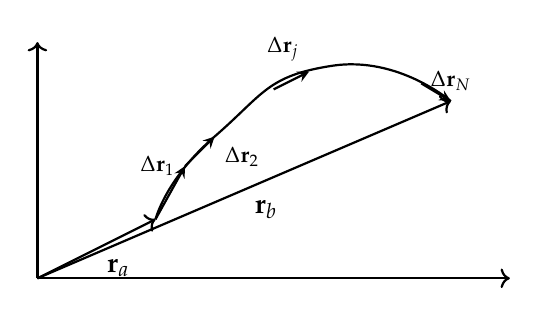
\begin{tikzpicture}[scale=1.5, thick]
    % Axes
    \draw[->] (0,0) -- (0,2);
    \draw[->] (0,0) -- (4,0);
    
    % Trajectory curve
    \draw[smooth, tension=1] plot coordinates {(1,0.5) (1.5, 1.2) (2.5, 1.8) (3.5, 1.5)};
    
    % Vectors to start and end
    \draw[->] (0,0) -- (1,0.5) node[midway, below right] {$\mathbf{r}_a$};
    \draw[->] (0,0) -- (3.5, 1.5) node[midway, below right] {$\mathbf{r}_b$};
    
    % Tiny displacement vectors
    \draw[->, >=stealth] (1,0.5) -- (1.25, 0.95) node[left] {\footnotesize $\Delta\mathbf{r}_1$};
    \draw[->, >=stealth] (1.25, 0.95) -- (1.5, 1.2) node[below right] {\footnotesize $\Delta\mathbf{r}_2$};
    \draw[->, >=stealth] (2, 1.6) -- (2.3, 1.75) node[above left] {\footnotesize $\Delta\mathbf{r}_j$};
    \draw[->, >=stealth] (3.25, 1.65) -- (3.5, 1.5) node[above] {\footnotesize $\Delta\mathbf{r}_N$};
\end{tikzpicture}
\end{center}

And now take the limit as $N \to \infty$, $\Delta\vec{r}_j \to d\vec{r}$, and $\Delta t_j \to dt$ so that the sum becomes an integral along the contour. What are the limits of integration on each integral?
\textcolor{blue}{
\begin{align*}
    \int_{\vec{r}_a}^{\vec{r}_b} \vec{F}(\vec{r}) \cdot d\vec{r} &= \frac{m}{2} \int_{t_a}^{t_b} \frac{d}{dt}(v^2) \, dt \quad \text{\footnotesize{Solve integral on r.h.s.}} \\
    &= \frac{m}{2} (v_b^2 - v_a^2) = K_b - K_a = \Delta K \quad \text{\footnotesize{Do you recognize the result?}}
\end{align*}
}

\begin{itemize}
    \item Both sides of the equation are valid in 3D.
    \item The l.h.s. is a ``line integral'' over the particle's specific trajectory in 3D.
    \item The r.h.s. involves the squares of the 3D velocities: $v^2 = v_x^2 + v_y^2 + v_z^2$.
    \item The value of the line integral $\int_{\vec{r}_a}^{\vec{r}_b} \vec{F}(\vec{r}) \cdot d\vec{r}$ is called the \textit{work} done by the net force $\vec{F}$ on the particle as the particle moves from $a$ to $b$ along a \textit{specified} path, and is denoted by $W_{ba}$:
    \[ W_{ba} \equiv \int_{\vec{r}_a}^{\vec{r}_b} \vec{F}(\vec{r}) \cdot d\vec{r}. \]
    \textcolor{blue}{Quick Question: Can work be both positive and negative? \textbf{Yes! It depends on the angle between force and displacement.}}
    \item The quantity $\frac{1}{2}mv^2$ is called the \textit{kinetic energy}\footnote{The concept of kinetic energy (with a role that is distinct from momentum) was introduced by \'Emilie du Ch\^atelet in her commentary on Isaac Newton's 1687 book \textit{Philosophiae Naturalis Principia Mathematica} while translating it into French in the 1740's. Her commentary includes a key contribution to Newtonian mechanics -- the postulate of an additional conservation law for total energy (which we will soon discover), of which kinetic energy is one element. See \url{https://en.wikipedia.org/wiki/Emilie_du_Chatelet} (look for the section on ``Advocacy of kinetic energy'').} and is denoted by $K$:
    \[ K \equiv \frac{1}{2}mv^2. \]
\end{itemize}

$\implies$ With these definitions, the expression we found above, $\int_{\vec{r}_a}^{\vec{r}_b} \vec{F}(\vec{r}) \cdot d\vec{r} = \frac{m}{2}(v_b^2 - v_a^2)$, can be written as
\[ W_{ba} = K_b - K_a, \text{ where } K_i = \frac{1}{2}mv_i^2. \]

This is called the ``\textbf{work-energy theorem}'': The work done on the particle as it moves from $a$ to $b$ along a \textit{specified} path is equal to the change in kinetic energy of the particle between the beginning and end of the path.

Note that this ``theorem'' is just another manifestation of Newton's 2nd Law. It provides yet another tool for our toolbox. We will now explore when \textit{and why} this is a particularly \textit{useful} tool.

\begin{exercise}[Exercise 2]
Write two expressions for the work $W_{\Delta\vec{r}}$ done by a force $\vec{F}$ during a small displacement $\Delta\vec{r}$ in terms of quantities shown in the figure below.
\begin{center}
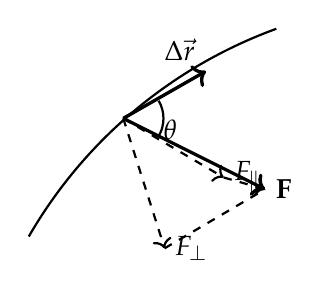
\begin{tikzpicture}[scale=1.5, thick]
    % Path curve
    \draw (0,0) arc (150:110:4);
    
    % Vectors
    \draw[->, very thick] (0.8, 1) -- (1.5, 1.4) node[above left] {$\Delta\vec{r}$};
    \draw[->, very thick] (0.8, 1) -- (2, 0.4) node[right] {$\mathbf{F}$};
    
    % Components
    \draw[dashed, ->] (0.8, 1) -- (1.65, 0.5) node[right] {$F_{\parallel}$};
    \draw[dashed, ->] (1.65, 0.5) -- (2, 0.4);
    \draw[dashed, ->] (0.8, 1) -- (1.15, -0.1) node[right] {$F_{\perp}$};
    \draw[dashed] (1.15, -0.1) -- (2, 0.4);
    
    % Angle
    \draw (1.1, 1.15) arc (30:-30:0.3);
    \node at (1.2, 0.9) {$\theta$};
\end{tikzpicture}
\end{center}
\textcolor{blue}{\[ W_{\Delta\vec{r}} = \vec{F} \cdot \Delta\vec{r} = F_{\parallel}\Delta r = F\Delta r\cos\theta \]}
$\implies$ The component of $\vec{F}$ \textbf{\textcolor{blue}{perpendicular}} to $\Delta\vec{r}$ does \textit{no} work.
\end{exercise}

From the definition of work in terms of a path integral, it appears that we need to know the exact path to use the equation -- but we often \textit{don't know} the path! There are two important cases when the work-energy theorem is nonetheless useful.
\begin{enumerate}
    \item For certain physical situations the path is \textit{constrained} so that we \textit{know} the path; in these cases, there may exist certain forces that do no work because they are perpendicular to the path.
    \item For certain types of forces, $W_{ba}$ is \textit{independent of the path}.
\end{enumerate}

\begin{exercise}[Exercise 3]
Here we give two examples of ``constrained'' motion. For each example,
\begin{enumerate}[label=\alph*.]
    \item Identify the forces acting on the body.
    \item State whether each force does or does \textit{not} do work on the object by considering $\vec{F} \cdot \Delta\vec{r}$ for each force.
    \item If the work done by a force is non-zero, what can you say about whether it is positive or negative?
\end{enumerate}

\textbf{I. The conical pendulum we considered in an earlier exercise.} \\
First assume no drag force. Then consider the case where drag is not negligible.
\begin{center}
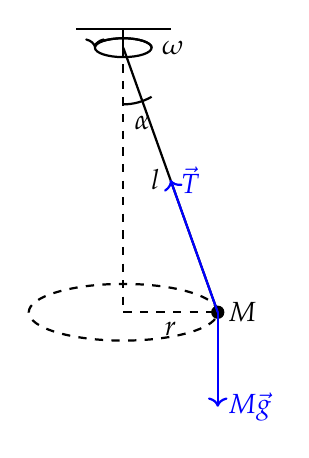
\begin{tikzpicture}[scale=1.2, thick]
    % Support
    \draw (-0.5, 2) -- (0.5, 2);
    \draw (0, 2) -- (0, 1.8);
    \draw (0, 1.8) ellipse (0.3 and 0.1);
    \draw[->] (0.3, 1.8) arc (0:180:0.3 and 0.1);
    \node[right] at (0.3, 1.8) {$\omega$};
    
    % Pendulum
    \draw[dashed] (0, 1.8) -- (0, -1);
    \draw (0, 1.8) -- (1, -1) node[midway, left] {$l$};
    \fill (1, -1) circle (2pt) node[right] {$M$};
    
    % Angle
    \draw (0, 1.2) arc (270:300:0.6);
    \node at (0.2, 1) {$\alpha$};
    
    % Path
    \draw[dashed] (0, -1) ellipse (1 and 0.3);
    \draw[dashed] (0, -1) -- (1, -1) node[midway, below] {$r$};
    
    % Forces
    \draw[->, color=blue] (1, -1) -- (0.5, 0.4) node[right] {$\vec{T}$};
    \draw[->, color=blue] (1, -1) -- (1, -2) node[right] {$M\vec{g}$};
\end{tikzpicture}
\end{center}
\textcolor{blue}{
\textbf{Case 1: No drag}
\begin{enumerate}[label=\alph*.]
    \item Forces: Gravity ($M\vec{g}$) and Tension ($\vec{T}$).
    \item Gravity points purely vertically, and the motion $\Delta\vec{r}$ is purely horizontal. Tension acts perpendicular to the circular path at all times. Therefore, neither force does any work! $W = 0$.
    \item N/A (Work is zero). Since $W = \Delta K = 0$, speed $v$ is constant.
\end{enumerate}
\textbf{Case 2: Drag is not negligible}
\begin{enumerate}[label=\alph*.]
    \item Forces: Gravity ($M\vec{g}$), Tension ($\vec{T}$), and Drag ($\vec{F}_D$).
    \item Gravity and Tension still do no work. Drag \textit{does} work, because it points anti-parallel to the velocity vector $\Delta\vec{r}$.
    \item The work done by drag is \textbf{negative} ($W < 0$), which will decrease the kinetic energy of the mass over time.
\end{enumerate}
}

\textbf{II. A roller coaster car that does loop-the-loops, corkscrews, ...} \\
Make a sketch of the car at a couple of points and the forces acting on it.
\begin{center}
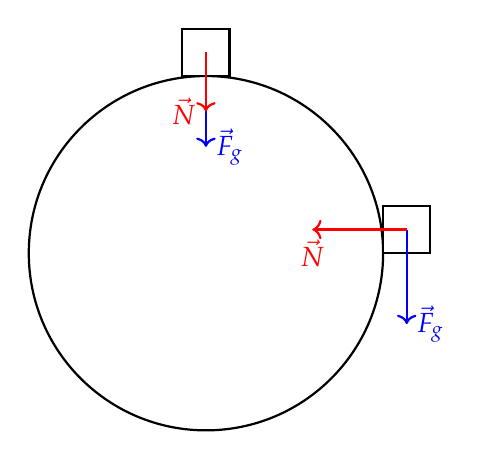
\begin{tikzpicture}[scale=1.5, thick]
    % Loop
    \draw (0,0) arc (180:0:1.5); % Top half
    \draw (0,0) arc (180:270:1.5); % Bottom left
    \draw (3,0) arc (0:-90:1.5); % Bottom right
    
    % Car at 3 o'clock
    \draw[fill=white] (3, 0) rectangle (3.4, 0.4);
    \draw[->, color=blue] (3.2, 0.2) -- (3.2, -0.6) node[right] {$\vec{F}_g$};
    \draw[->, color=red] (3.2, 0.2) -- (2.4, 0.2) node[below] {$\vec{N}$};
    
    % Car at 12 o'clock
    \draw[fill=white] (1.3, 1.5) rectangle (1.7, 1.9);
    \draw[->, color=blue] (1.5, 1.7) -- (1.5, 0.9) node[right] {$\vec{F}_g$};
    \draw[->, color=red] (1.5, 1.7) -- (1.5, 1.2) node[left] {$\vec{N}$};
\end{tikzpicture}
\end{center}
\textcolor{blue}{
\begin{enumerate}[label=\alph*.]
    \item Forces: Gravity ($\vec{F}_g$) and the Normal force ($\vec{N}$) from the track.
    \item The Normal force is always perpendicular to the track (the path $\Delta\vec{r}$), so it does \textit{no work}. Gravity has a component along the path during the ascent and descent, so it \textit{does work}.
    \item The work done by gravity can be \textbf{both}. As the car goes down, $\vec{F}_g \cdot \Delta\vec{r} > 0$ (positive work, speed increases). As the car goes up the loop, $\vec{F}_g \cdot \Delta\vec{r} < 0$ (negative work, speed decreases).
\end{enumerate}
}
\end{exercise}

% ==================== LECTURE 23 ====================
\chapter{Conservative Forces \& Potential Energy}

\section*{Conservative Forces}

We'll now consider a special class of forces called ``conservative forces.''
\begin{itemize}
    \item Consider the work $W_{ba}$ done by a force $\vec{F}(\vec{r})$ on an object that follows a path from $\vec{r}_a$ at time $t_a$ to $\vec{r}_b$ at time $t_b$.
    \item If $W_{ba}$ is \textit{independent} of the path between $\vec{r}_a$ and $\vec{r}_b$, then the force is called a \textit{conservative} force.
\end{itemize}

Let's start by considering the one-dimensional case where $\vec{F}(x) = F_x(x)\hat{i}$. In 1D, the work done by a \textit{conservative} force on an object that follows a path from $x_a$ to $x_b$ is independent of the path between $x_a$ and $x_b$ and can therefore be written as
\[ W_{ba} = \int_{x_a}^{x_b} F_x(x)\,dx. \quad \text{\footnotesize{Note that this is no longer a \textit{line} integral.}} \]

\textcolor{blue}{\textbf{Quick Exercise:} Sketch a few examples of ``different paths'' between two points in 1D. \\
\textit{For example, a particle could go straight from $x_a$ to $x_b$, or it could overshoot $x_b$, turn around, and come back. In 1D, these are the only ways to vary the path!}}

Path independence is equivalent to saying that $W_{ba}$ can be written as the \textit{difference} between a function evaluated at $x_b$ and at $x_a$. Call this function $-U(x)$. (The reason for the negative sign will become apparent soon!) We can then write this condition as
\[ W_{ba} = \int_{x_a}^{x_b} F_x(x)\,dx = -U(x_b) + U(x_a) = -\Big(U(x_b) - U(x_a)\Big). \tag{1} \]
\begin{itemize}
    \item The function $U(x)$ has the same dimensions as work and kinetic energy -- i.e., dimensions of energy.
    \item $U(x)$ is called the ``\textbf{potential energy function}'' associated with the physical system.
    \begin{itemize}
        \item The \textit{system} consists of whatever is causing the force, and the object that is experiencing the force.
    \end{itemize}
\end{itemize}

\textcolor{blue}{\textbf{Quick Questions:} If $\vec{F}$ is a conservative force, then \dots}
\begin{enumerate}
    \item How is $W_{ba}$ related to $W_{ab}$? \\
    \textcolor{blue}{\[ W_{ba} = -W_{ab} \]}
    \item What is the work done around a closed path -- i.e., points $a$ and $b$ are at the same position? \\
    \textcolor{blue}{\[ 0 \]}
\end{enumerate}

\section*{Conservation of Mechanical Energy}

In the previous lecture, we derived the ``\textbf{work-energy theorem}:''
\[ W_{ba} = K_b - K_a. \]

\begin{exercise}[Exercise 1]
Write the work-energy theorem for the special case in which \textit{only} conservative forces act on the mass $m$. \\
\textcolor{blue}{
\[ K_b - K_a = -U_b + U_a \]
}
Now write the relation in a form that makes evident a \textbf{conserved} quantity: \\
\textcolor{blue}{
\[ K_b + U_b = K_a + U_a \implies E_A = E_B \]
}
\end{exercise}

We denote this conserved quantity by $E$ and call it the \textit{total mechanical energy}:
\textcolor{blue}{\[ E = K + U \]}

Since $E$ is independent of the position of the particle, it is a \textit{conserved} quantity. This is why we called this particular type of force a \textit{conservative} force.

\begin{exercise}[Exercise 2]
Identify two common physical examples of ``conservative'' forces in one dimension. For each example,
\begin{enumerate}[label=(\alph*)]
    \item define the direction and origin of the coordinate axis in 1D;
    \item write an expression for the force component and make a sketch of the function;
    \item find the expression for $W_{ba}$ by doing an explicit integral; and
    \item by comparing your result for $W_{ba}$ to equation 1, identify the function $U$, and then sketch it.
\end{enumerate}

\begin{itemize}
    \item Example 1: \textcolor{blue}{\textbf{Gravity (near Earth's surface)}}
    \textcolor{blue}{
    \begin{itemize}
        \item Let the $y$-axis point \textit{downwards}. The force is $F_y = mg$.
        \item $W_{ba} = \int_{y_1}^{y_2} mg\,dy = mg(y_2 - y_1) = mg\Delta y$.
        \item Since $W_{ba} = -(U(y_2) - U(y_1))$, we identify $U(y) = -mgy$. (If we chose $y$ pointing up, $F_y = -mg$, $W_{ba} = -mg\Delta y$, and $U(y) = mgy$).
    \end{itemize}
    }
    
    \item Example 2: \textcolor{blue}{\textbf{Electric Repulsion}}
    \textcolor{blue}{
    \begin{itemize}
        \item Two positive charges $q_1$ and $q_2$. Let $q_1$ be at the origin, and $q_2$ at position $x$.
        \item $F_x = \frac{1}{4\pi\varepsilon_0}\frac{q_1 q_2}{x^2}$.
        \item $W_{ba} = \int_{x_1}^{x_2} \frac{1}{4\pi\varepsilon_0}\frac{q_1 q_2}{x^2}\,dx = -\frac{q_1 q_2}{4\pi\varepsilon_0}\left( \frac{1}{x_2} - \frac{1}{x_1} \right)$.
        \item Comparing to $W_{ba} = -(U_2 - U_1)$, we identify $U(x) = \frac{q_1 q_2}{4\pi\varepsilon_0 x}$.
    \end{itemize}
    }
\end{itemize}
\end{exercise}

\section*{Calculating Force from a Potential Energy Function}

For a conservative force in one dimension, the potential energy difference is given by the negative integral of the force $F_x(x)$:
\[ U(x_b) - U(x_a) = -\int_{x_a}^{x_b} F_x(x)\,dx. \implies U(x) \text{ is the \textit{antiderivative} of } -F_x(x). \]

Therefore, $F_x(x)$ is the derivative of the negative potential energy function:
\textcolor{blue}{\[ F_x(x) = -\frac{dU}{dx} \]}

Try it:
\[ -\int_{x_a}^{x_b} F_x(x)\,dx = -\int_{x_a}^{x_b} \left( -\frac{dU}{dx} \right)\,dx = U(x_b) - U(x_a). \]

\begin{exercise}[Exercise 3]
Check that the above relationship holds for the spring force $F_{\text{sp},x}$ and the potential energy function $U_{\text{sp}}(x)$. \\
\textcolor{blue}{
\[ -\int_{x_a}^{x_b} (-kx)\,dx = \frac{1}{2}k(x_b^2 - x_a^2) = \frac{1}{2}kx_b^2 - \frac{1}{2}kx_a^2 = U(x_b) - U(x_a) \]}

What is $d^2U_{\text{sp}}/dx^2$ for this potential? Interpret. \\
\textcolor{blue}{\[ \frac{d^2U}{dx^2} = \frac{d^2}{dx^2}\left(\frac{1}{2}kx^2\right) = \frac{d}{dx}(kx) = k. \]}
\end{exercise}

In Lecture 19 (Differential Equations in Mechanics II), we considered a linear restoring (`spring') force $F_x(x)$ and found the general solution for $x(t)$ expressed as a sum of sine and cosine functions (or a sum of exponentials with imaginary exponents) with angular frequency $\omega = \sqrt{\frac{k}{m}}$ or $\omega^2 = \frac{k}{m}$. Combining this with $k = \frac{d^2U_{\text{sp}}}{dx^2}$ from the above exercise, we find that
\[ \omega^2 = \frac{1}{m}\frac{d^2U_{\text{sp}}}{dx^2}. \]
These results will be very relevant for the next Exercise and problems on Problem Set 8.

\begin{exercise}[Exercise 4: Energy Diagrams for a 1D Conservative Potential]
\begin{itemize}
    \item Work on a whiteboard with your group to respond to the questions presented on the slides (in class).
    \item Topics addressed: Starting with a 1D potential energy function, sketch the force, identify points of stable or unstable \textbf{\textcolor{blue}{equilibrium}}, and identify regions in which bound states can exist.
\end{itemize}
\end{exercise}

\section*{Central forces}

In this section, we'll calculate $W_{ba}$ for an important class of conservative forces in \textbf{three dimensions} called ``\textit{central forces}''.

A central force is a radial force that depends only on the distance $r$ from the origin:
\[ \vec{F} = f(r)\hat{r}. \]

\begin{exercise}[Exercise 5]
\textbf{General case of a central force}
\begin{itemize}
    \item In this exercise, you'll find the work done by the central force $\vec{F} = f(r)\hat{r}$ on a particle that moves from $\vec{r}_a$ to $\vec{r}_b$.
    \item For simplicity, consider motion in a plane containing the origin so that we can use polar coordinates.
\end{itemize}

\begin{enumerate}[label=(\alph*)]
    \item Express $d\vec{r}$ in polar coordinates. (Try to recall the expression using simple dimensional analysis and possibly a sketch.) \\
    \textcolor{blue}{\[ d\vec{r} = dr\,\hat{r} + r\,d\theta\,\hat{\theta} \]}
    
    \item Now calculate $W_{ba}$ for $\vec{F} = f(r)\hat{r}$:
    \[ W_{ba} = \int_{\vec{r}_a}^{\vec{r}_b} \vec{F} \cdot d\vec{r} \]
    \textcolor{blue}{
    \begin{align*}
        W_{ba} &= \int_{\vec{r}_a}^{\vec{r}_b} \left( f(r)\hat{r} \right) \cdot \left( dr\,\hat{r} + r\,d\theta\,\hat{\theta} \right) \\
        &= \int_{r_a}^{r_b} f(r)\,dr \\
        &= F(r_b) - F(r_a) \quad \text{\footnotesize{(where $F$ is the antiderivative of $f$)}}
    \end{align*}
    }
    
    \item Based on your result, what can you conclude about the work done by a central force -- in particular, what does $W_{ba}$ depend on, and what does it \textit{not} depend on? \\
    \textcolor{blue}{\textbf{It does not depend on the path. It only depends on the starting and ending radii ($r_a$ and $r_b$).}}
\end{enumerate}
\end{exercise}

\begin{exercise}[Exercise 6]
\textbf{Gravitational force $\vec{F}_G$ -- important example of a central force!} \\
In this exercise, you will calculate the work done by the gravitational force of the Earth on an object of mass $m$ that moves from radius $r_a$ to radius $r_b$, where $r_a$ and/or $r_b$ are not necessarily close to the radius of the Earth, $R_E$. You will then apply the work-energy theorem to calculate the escape velocity from Earth. \textbf{\textcolor{red}{Do this exercise on your whiteboard; share the marker.}}
\begin{enumerate}[label=(\alph*)]
    \item Write the equation for the force of gravity, $\vec{F}_G$, on the mass $m$. (Yes, write it as a vector.) \\
    \textcolor{blue}{\[ \vec{F}_g = -G\frac{M_E m}{r^2}\hat{r} \]}
    
    \item Use the result from the previous exercise for a general central force to find $W_{ba}$ for the case of gravity. \\
    \textcolor{blue}{
    \begin{align*}
        W_{ba} &= \int_{r_a}^{r_b} \left( -G\frac{M_E m}{r^2} \right) dr = \left[ G\frac{M_E m}{r} \right]_{r_a}^{r_b} \\
        &= G\frac{M_E m}{r_b} - G\frac{M_E m}{r_a} = GM_E m\left( \frac{1}{r_b} - \frac{1}{r_a} \right)
    \end{align*}
    (If $r_b > r_a$, then $1/r_b < 1/r_a$, so the work done by gravity is negative, as expected.)
    }
    
    \item Based on your result in part (b), identify the expression for $U_G(r)$. What is the value of $U_G(r)$ as $r \to \infty$? Sketch the potential energy function $U_G(r)$. \\
    \textcolor{blue}{
    Since $W_{ba} = -(U(r_b) - U(r_a))$, we see that:
    \[ U_G(r) = -G\frac{M_E m}{r} \]
    As $r \to \infty$, $U_G(r) \to 0$. The sketch of $U_G(r)$ is a $1/r$ curve in the 4th quadrant, asymptotically approaching the $r$-axis from below.
    }
    
    \item The work-energy theorem for conservative forces led to a conserved quantity. What is the conserved quantity? \\
    \textcolor{blue}{\textbf{Total Mechanical Energy} ($E = K + U$).} \\
    You will now use this conserved quantity to find the ``escape velocity'' $v_a = v_{\text{esc}}$ from the surface of the Earth ($r_a = R_E$) for mass $m$, neglecting drag.
    \begin{itemize}
        \item Quick question -- How is ``escape velocity defined''? \textit{Hint:} How should we define $r_b$ and $v_b$? \\
        \textcolor{blue}{
        Escape velocity is the minimum speed needed to reach $r_b \to \infty$ with $v_b \ge 0$. Let's set the limiting case where it barely reaches infinity with zero speed: $v_b = 0$ at $r_b = \infty$.
        \begin{align*}
            K_a + U(r_a) &= K_b + U(r_b) \\
            \frac{1}{2}m v_{\text{esc}}^2 - \frac{GM_E m}{R_E} &= 0 + 0 \\
            v_{\text{esc}} &= \sqrt{\frac{2GM_E}{R_E}}
        \end{align*}
        }
    \end{itemize}
    
    \item Does the escape velocity depend on the mass of the object being launched? \\
    Does it depend on the launch angle? \\
    \textcolor{blue}{\textbf{No} (mass $m$ cancels out). \\
    \textbf{No} (kinetic energy is a scalar depending only on the magnitude of velocity, though practically you can't launch horizontally into the ground!).}
    
    \item Speculate on the physics reason for why satellites launched in the U.S. are usually launched in a trajectory toward the east from Cape Canaveral FL, or from south Texas. \\
    \textcolor{blue}{The Earth is spinning towards the east. By launching eastwards (especially near the equator), the rocket starts with a ``free'' initial velocity $v_0$ from the Earth's rotation, requiring less fuel to reach orbital or escape velocity.}
\end{enumerate}
\end{exercise}

% ==================== LECTURE 24 ====================
\chapter{3D Conservative Forces; Non-Conserv. Forces}

In Lecture 23, we introduced the \textbf{1D} potential energy function $U(x)$ associated with a conservative force $F_x$. $U(x)$ is defined (up to an arbitrary constant) through these relationships:
\[ U(x_b) - U(x_a) = -\int_{x_a}^{x_b} F_x(x)\,dx \implies F_x(x) = -\frac{dU(x)}{dx}. \tag{1} \]

If instead we start with the integral formulation for potential energy in \textbf{three dimensions}, what is the 3D version of equation 1?
\[ U(\vec{r}_b) - U(\vec{r}_a) = -\int_{\vec{r}_a}^{\vec{r}_b} \vec{F}(\vec{r}) \cdot d\vec{r} \implies \vec{F}(\vec{r}) = \text{??} \]

Start by computing the change in potential energy across a small change in position \textit{along only one direction} -- say the $x$ direction (in Cartesian coordinates): $d\vec{r} = dx\,\hat{i}$.

\begin{exercise}[Exercise 1]
Add any missing limits of integration on the integrals and then write the final result in the last line.
\textcolor{blue}{
\begin{align*}
    U(x + \Delta x, y, z) - U(x, y, z) &= -\int_{(x,y,z)}^{(x+\Delta x, y, z)} \vec{F} \cdot d\vec{r} \quad \text{\footnotesize{Use $d\vec{r} = dx\,\hat{i}$}} \\
    &= -\int_x^{x+\Delta x} F_x\,dx \quad \text{\footnotesize{$F_x \sim$ constant over interval $dx$}} \\
    &\simeq -F_x \Delta x
\end{align*}
\[ \implies F_x \simeq -\frac{U(x + \Delta x, y, z) - U(x, y, z)}{\Delta x} \]
\[ \text{Take limit as } \Delta x \to 0: \quad F_x = -\frac{\partial U}{\partial x} \]
}
\end{exercise}

We can repeat this derivation for the $y$ and $z$ directions to find
\textcolor{blue}{\[ \vec{F} = -\nabla U(\vec{r}) = \left( -\frac{\partial U}{\partial x}, -\frac{\partial U}{\partial y}, -\frac{\partial U}{\partial z} \right) \]}

\begin{exercise}[Exercise 2]
In each of the following statements, circle the correct word or fill in the blank. (Use what your group can recall about the gradient operator.)
\begin{itemize}
    \item The gradient of $U(\vec{r})$ points in the direction of steepest \textcolor{blue}{\textbf{ascent}} / descent of $U(\vec{r})$.
    \item The force points in the direction of steepest ascent / \textcolor{blue}{\textbf{descent}} of the potential energy.
    \item Given $U(\vec{r})$, the component of the force in a given direction $\hat{n}$ is $\vec{F} \cdot \hat{n} = \textcolor{blue}{\mathbf{-\nabla U(\vec{r}) \cdot \hat{n}}}$
    \item If the potential is constant (`flat') in a particular direction, the component of the force in that direction is \textcolor{blue}{\textbf{0}}.
    \item The force is always parallel / \textcolor{blue}{\textbf{perpendicular}} to surfaces (in 3D) of constant potential energy.
\end{itemize}
\end{exercise}

\begin{exercise}[Exercise 3]
Consider the following potential energy function in two dimensions:
\[ U(x,y) = k(x^2 + 2y^2) \]
\begin{enumerate}
    \item Write an expression for the force $\vec{F}(x,y)$. \\
    \textcolor{blue}{\[ \vec{F} = -\nabla U = -2k(x\,\hat{i} + 2y\,\hat{j}) \]}
    
    \item On your whiteboard, sketch a \textit{contour plot} of $U$ (with at least three contour lines of constant $U$) in the $x-y$ plane.
    \begin{enumerate}[label=(\alph*)]
        \item Draw contours corresponding to \textbf{equally spaced values} of constant $U$.
        \item Now draw a \textit{vector plot} of $\vec{F}$ on the same plane. Indicate the relative magnitude of $\vec{F}$ with the length of the vector.
        \item Specify whether you are assuming that the constant $k$ is positive or negative. Articulate what would change in your sketch if you made the opposite assumption.
    \end{enumerate}
\end{enumerate}
\begin{center}
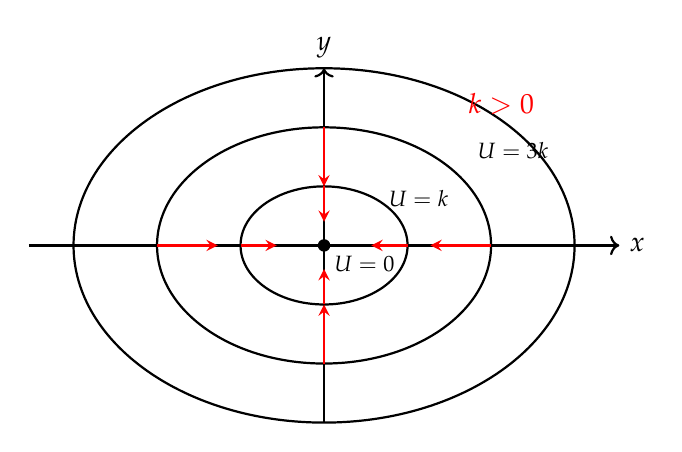
\begin{tikzpicture}[scale=1.5, thick]
    % Axes
    \draw[->] (-2.5, 0) -- (2.5, 0) node[right] {$x$};
    \draw[->] (0, -1.5) -- (0, 1.5) node[above] {$y$};
    
    % Contours
    \draw (0,0) ellipse (0.707 and 0.5); % U = k
    \draw (0,0) ellipse (1.414 and 1.0); % U = 2k
    \draw (0,0) ellipse (2.121 and 1.5); % U = 3k
    
    % Labels
    \fill (0,0) circle (1.5pt) node[below right] {\footnotesize $U=0$};
    \node at (0.8, 0.4) {\footnotesize $U=k$};
    \node at (1.6, 0.8) {\footnotesize $U=3k$};
    \node[text=red] at (1.5, 1.2) {$k > 0$};
    
    % Vectors (Force points INWARD for k > 0)
    \draw[->, color=red, >=stealth] (0.707, 0) -- (0.4, 0);
    \draw[->, color=red, >=stealth] (-0.707, 0) -- (-0.4, 0);
    \draw[->, color=red, >=stealth] (0, 0.5) -- (0, 0.2);
    \draw[->, color=red, >=stealth] (0, -0.5) -- (0, -0.2);
    
    \draw[->, color=red, >=stealth] (1.414, 0) -- (0.9, 0);
    \draw[->, color=red, >=stealth] (-1.414, 0) -- (-0.9, 0);
    \draw[->, color=red, >=stealth] (0, 1.0) -- (0, 0.5);
    \draw[->, color=red, >=stealth] (0, -1.0) -- (0, -0.5);
\end{tikzpicture}
\end{center}
\textcolor{blue}{The contours are ellipses. Because $y$ has a larger coefficient, the ellipses are compressed along the $y$-axis. Assuming $k>0$, the potential increases as you move away from the origin, so the force vectors point \textbf{inward} (down the gradient) and are perpendicular to the contour lines. If $k<0$, the force vectors would point \textbf{outward}.}
\end{exercise}

\begin{exercise}[Exercise 4]
Consider the contour plot below, which represents an ``effective'' potential energy function in a non-inertial frame.
\begin{itemize}
    \item The empty `holes' in the diagram are near the locations of two massive objects of unequal mass, with the more massive object on the left.
    \item Physically, this contour map depicts what is called an \textit{effective} gravitational potential energy in the region near a stable two-body orbiting system in a \textit{rotating} (i.e., non-inertial!) reference frame. The origin corresponds to the center of mass (CM) of the two-body system.
    \item For example, the central body could be the Earth and the orbiting body the Moon, or the central body could be the Sun and the other body any orbiting planet.
\end{itemize}

\begin{center}
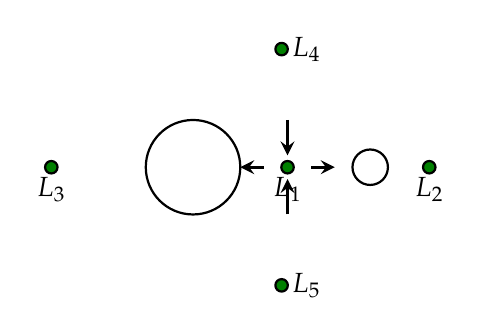
\begin{tikzpicture}[scale=1.5, thick]
    % Central mass
    \draw[fill=white] (-0.3, 0) circle (0.4);
    % Smaller mass
    \draw[fill=white] (1.2, 0) circle (0.15);
    
    % Equilibrium points (Lagrange points)
    \filldraw[fill=green!50!black] (0.5, 0) circle (1.5pt) node[below] {$L_1$};
    \filldraw[fill=green!50!black] (1.7, 0) circle (1.5pt) node[below] {$L_2$};
    \filldraw[fill=green!50!black] (-1.5, 0) circle (1.5pt) node[below] {$L_3$};
    \filldraw[fill=green!50!black] (0.45, 1.0) circle (1.5pt) node[right] {$L_4$};
    \filldraw[fill=green!50!black] (0.45, -1.0) circle (1.5pt) node[right] {$L_5$};
    
    % Force vectors around L1 (Saddle point)
    \draw[->, >=stealth, very thick] (0.3, 0) -- (0.1, 0);
    \draw[->, >=stealth, very thick] (0.7, 0) -- (0.9, 0);
    \draw[->, >=stealth, very thick] (0.5, 0.4) -- (0.5, 0.1);
    \draw[->, >=stealth, very thick] (0.5, -0.4) -- (0.5, -0.1);
\end{tikzpicture}
\end{center}

\begin{enumerate}
    \item Directly on the plot, indicate with a dot any points of equilibrium. \\
    \textcolor{blue}{\textbf{Done.} (These are the 5 Lagrange points: $L_1$ through $L_5$).}
    \item Draw force vectors in the region near each equilibrium point. \\
    \textcolor{blue}{\textbf{See $L_1$ above.} The arrows point towards the massive bodies (downhill into the gravity wells) along the $x$-axis, but inwards towards the saddle point along the $y$-axis.}
    \item Indicate whether each equilibrium point is stable (S) or unstable (U) in each direction. \\
    \textcolor{blue}{\textbf{$L_1, L_2$, and $L_3$ are saddle points}: Unstable along the horizontal axis, but stable along the vertical axis.}
\end{enumerate}
\end{exercise}

\section*{Non-conservative Forces}

As we argued above, the work done on a particle by a \textit{conservative} force is path independent or, equivalently, the work done on the particle as it executes a closed path is 0.

\begin{exercise}[Exercise 5]
Give two examples of physical \textit{non-conservative} forces. \\
\textcolor{blue}{\textbf{Friction, Drag}}
\end{exercise}

\begin{exercise}[Exercise 6]
Sketch at least one example of a force field $\vec{F}(\vec{r})$ in two dimensions for which you are able to predict that the work done by $\vec{F}$ is \textit{not} path independent or, equivalently, that the work done as a particle executes a closed path is \textit{not} 0.
\begin{center}
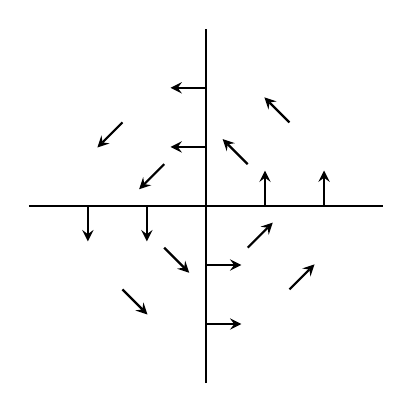
\begin{tikzpicture}[scale=1.5, thick]
    % Axes
    \draw (-1.5, 0) -- (1.5, 0);
    \draw (0, -1.5) -- (0, 1.5);
    
    % Swirl / Vortex
    \foreach \r in {0.5, 1.0} {
        \foreach \a in {0, 45, 90, 135, 180, 225, 270, 315} {
            \draw[->, >=stealth] (\a:\r) -- ++(\a+90:0.3);
        }
    }
\end{tikzpicture}
\end{center}
\textcolor{blue}{A \textbf{vortex} or swirling vector field. If you integrate the force along a circular path following the arrows, the work is strictly positive and does not equal zero for a closed loop.}
\end{exercise}

Often both conservative forces $\vec{F}^c$ and non-conservative forces $\vec{F}^{nc}$ act on the same system. We can then write
\[ \vec{F} = \vec{F}^c + \vec{F}^{nc}. \]
Since the \textit{work-energy theorem} is true whether or not the forces are conservative, the total work done by $\vec{F}$ as the particle moves from $a$ to $b$ is
\begin{align*}
    W_{ba}^{\text{total}} &= \int_{\vec{r}_a}^{\vec{r}_b} \vec{F} \cdot d\vec{r} \\
    &= \int_{\vec{r}_a}^{\vec{r}_b} \vec{F}^c \cdot d\vec{r} + \int_{\vec{r}_a}^{\vec{r}_b} \vec{F}^{nc} \cdot d\vec{r} \\
    &= -U_b + U_a + W_{ba}^{nc},
\end{align*}
where $U$ is the potential energy associated with the conservative force and $W_{ba}^{nc}$ is the work done on the particle by the non-conservative force. \textcolor{blue}{(Recall from vector calculus: $\nabla \times \vec{F} = \vec{0}$ for conservative forces).}

\begin{exercise}[Quick Exercise 7]
Use the work-energy theorem ($W_{ba}^{\text{total}} = K_b - K_a$) and the definition of mechanical energy ($E = K + U$) to write a generalization of the statement of conservation of mechanical energy. Check that all the relative signs make sense to you. \\
\textcolor{blue}{
\begin{align*}
    -U_b + U_a + W_{ba}^{nc} &= K_b - K_a \\
    W_{ba}^{nc} &= (K_b + U_b) - (K_a + U_a) \\
    W_{ba}^{nc} &= E_b - E_a \\
    \implies \Delta E &= W_{ba}^{nc}
\end{align*}
\textbf{The change in total mechanical energy is equal to the work done by non-conservative forces.}
}
\end{exercise}

\section*{Collisions}

\begin{itemize}
    \item Consider two identical balls of mass $m$ that collide in the $x-y$ plane, corresponding to the surface of a perfectly horizontal billiard table.
    \item Assume friction and drag \textbf{before} and \textbf{after} the collision can be neglected.
\end{itemize}

\textbf{Questions:}
\begin{enumerate}[label=(\roman*)]
    \item Is the total momentum of the two balls conserved? Why or why not? \\
    \textcolor{blue}{\textbf{Yes. There are no external forces acting on the system in the $x-y$ plane.}}
    
    \item Is the total kinetic energy of the two balls necessarily conserved? Why or why not? (Consider the time before, during, and after the collision separately.) \\
    \textcolor{blue}{\textbf{No.} During the collision, energy can be lost to heat (non-conservative work due to internal friction/deformation) or sound.}
    
    \item How are each of the following types of collisions defined?
    \begin{itemize}
        \item \textbf{Elastic collision:} \\
        \textcolor{blue}{$\vec{P}$ conserved, $K$ conserved}
        \item \textbf{Inelastic collision:} \\
        \textcolor{blue}{$\vec{P}$ conserved, $K$ decreases}
        \item \textbf{Completely (or totally) inelastic collision:} \\
        \textcolor{blue}{$\vec{P}$ conserved, $K$ decreases, and the objects stick together}
        \item \textbf{Explosive collision:} \\
        \textcolor{blue}{$\vec{P}$ conserved, $K$ increases (e.g. stored potential energy is released)}
    \end{itemize}
\end{enumerate}

You will apply these concepts in collision problems on Problem Set 8.

% ==================== LECTURE 25 ====================
\chapter{Angular Momentum \& Torque}

Ch.\,7 (Angular Momentum \& Fixed Axis Rotation) in Kleppner \& Kolenkow.

In the past two weeks, we re-framed Newton's Laws twice: first in terms of momentum and then in terms of work and energy, giving us new useful tools, as well as two conserved quantities -- in specific situations:
\begin{itemize}
    \item conservation of total momentum $\vec{P}$ for an isolated system;
    \item conservation of total mechanical energy $E = K + U$ for conservative forces.
\end{itemize}

Now we'll re-frame Newton's Laws yet again, this time to handle rotational motion. Just like we did with momentum, we'll start with a single point particle and gradually work up to extended objects. We'll start by \textbf{defining} two new quantities -- angular momentum and torque. We'll then rewrite Newton's 2nd Law in terms of these quantities. And of course we'll do everything in full vector notation!

\section*{1st Definition: Angular momentum for a point particle}

Consider a point particle with momentum $\vec{p}$ at position $\vec{r}$ with respect to the origin O of a coordinate system.

The instantaneous angular momentum $\vec{L}$ about O, for this particle, is defined as
\[ \vec{L} \equiv \vec{r} \times \vec{p}, \]
where the symbol $\times$ denotes the cross product.

\begin{exercise}[Exercise 1]
Write an expression for the magnitude of $\vec{L}$. (Do \textit{not} write it in terms of components of $\vec{r}$, $\vec{p}$, or $\vec{L}$.) \\
Describe the direction of $\vec{L}$. \\
\textcolor{blue}{
\[ L = r p \sin\phi \]
where $\phi$ is the angle between $\vec{r}$ and $\vec{p}$. The direction is given by the right-hand rule (e.g., if $\vec{r}$ is $\hat{i}$ and $\vec{p}$ is $\hat{j}$, $\vec{L}$ points in the $\hat{k}$ direction, out of the page $\odot$).
}
\end{exercise}

\textit{Important note:} We cannot meaningfully speak of the angular momentum of a particle alone; we must identify the point about which we are calculating $\vec{L}$.

\begin{exercise}[Exercise 2]
Indicate on the figures below two geometric interpretations of the result you wrote for the magnitude $L$ of the angular momentum. \\
\textit{Hint: Consider grouping different factors in the expression for $L$.} \\
\textcolor{blue}{
\textbf{Interpretation 1:} $L = r (p \sin\phi) = r p_\perp$ \\
Here, $p_\perp$ is the component of momentum perpendicular to the position vector $\vec{r}$. \\
\textbf{Interpretation 2:} $L = (r \sin\phi) p = r_\perp p$ \\
Here, $r_\perp$ (also called the `impact parameter' or `moment arm' $b$) is the perpendicular distance from the origin to the line of action of the momentum vector.
}
\end{exercise}

\begin{exercise}[Exercise 3]
The figures below show the paths taken by several particles.
\begin{itemize}
    \item In (a - d), they move with constant speed.
    \item In (e), the motion is back and forth.
\end{itemize}
(a) Circular path around an external origin O. \\
(b) Circular path passing through the origin O. \\
(c) Straight line trajectory pointing directly away from O. \\
(d) Straight line trajectory passing by O at a closest distance $b$. \\
(e) Back and forth line trajectory.

\begin{enumerate}[label=(\roman*)]
    \item With respect to the origin O, in which case(s) is the angular momentum zero for at least one point in time? \\
    \textcolor{blue}{\textbf{(b)}: $L=0$ when the particle passes through O ($\vec{r} = \vec{0}$). \\
    \textbf{(c)}: $L=0$ always, because $\vec{r}$ is parallel to $\vec{p}$ ($r_\perp = 0$). \\
    \textbf{(e)}: $L=0$ at the turn-around points because speed (and thus $p$) is zero.}
    
    \item In which case(s) is the angular momentum about O constant? \\
    \textcolor{blue}{\textbf{(c)} and \textbf{(d)}. These represent free particles (constant velocity, zero net force, zero net torque). In (c), $L=0$ always. In (d), $L=pb$ always. (Note: in (a), the net force points to the center of the circle, not to O, so there is a net torque about O, meaning $L$ changes).}
    
    \item Suppose the radius of the circle in (a) is $b$, and the distance of closest approach of the particle to the origin in (d) is also $b$. If the momentum of the particle is $p$ in each case, what is the value of $L$ for each case? \\
    \textcolor{blue}{
    For (a) at the point closest to O (distance $b$): $L = b p$. \\
    For (d): $L = b p$ (this is true at \textit{every} point on the line!).
    }
\end{enumerate}
\end{exercise}

\begin{exercise}[Exercise 4]
Consider the case when $\vec{r}$ and $\vec{p}$ both lie in the $x-y$ plane. Then
\begin{align*}
    \vec{L} = \vec{r} \times \vec{p} &= (x\hat{i} + y\hat{j}) \times (p_x\hat{i} + p_y\hat{j}) \\
    &= x\hat{i} \times p_y\hat{j} + y\hat{j} \times p_x\hat{i} \quad \text{\footnotesize{Used $\hat{i}\times\hat{i}=0$ and $\hat{j}\times\hat{j}=0$}}
\end{align*}
\textcolor{blue}{
\begin{align*}
    &= x p_y (\hat{i} \times \hat{j}) + y p_x (\hat{j} \times \hat{i}) \quad \text{\footnotesize{Use $\hat{i}\times\hat{j} = \hat{k}$ and $\hat{j}\times\hat{i} = -\hat{k}$}} \\
    &= x p_y \hat{k} - y p_x \hat{k} \\
    &= (x p_y - y p_x)\hat{k}
\end{align*}
}
The following figure appears on p.\,243 in the textbook by Kleppner \& Kolenkow. The point of the figure is to illustrate how we can use the above result to calculate $L_z$. Identify the \textit{error in the figure}, and complete the equation for $L_z$ below the right-hand panel. \\
\textcolor{blue}{
\textbf{Equation:} $L_z = x p_y - y p_x$. \\
\textbf{Error:} In the middle panel showing the $y p_x$ term, the dashed rotation arrow is drawn counter-clockwise. However, a momentum $p_x$ in the $+x$ direction at a positive $y$ position creates a \textbf{clockwise} angular momentum about the origin (hence the negative sign in $-y p_x$).
}
\end{exercise}

\begin{exercise}[Optional Exercise 5]
[Do this Exercise on your own \textit{if} you are already familiar with determinants.] Write $\vec{L} = \vec{r} \times \vec{p}$ as a determinant and use it to write $\vec{L}$ for $\vec{r}$ and $\vec{p}$ lying in the $x, y$ plane: $\vec{r} = x\hat{i} + y\hat{j}$ and $\vec{p} = p_x\hat{i} + p_y\hat{j}$. \\
\textcolor{blue}{
\[ \vec{L} = \begin{vmatrix} \hat{i} & \hat{j} & \hat{k} \\ x & y & 0 \\ p_x & p_y & 0 \end{vmatrix} = \hat{k}(x p_y - y p_x) \]
}
\end{exercise}

\section*{2nd Definition: Torque due to force acting on a point particle}

Definition of torque $\vec{\tau}$ about point O due to a force $\vec{F}$ acting on a particle at position $\vec{r}$ relative to O:
\[ \vec{\tau} \equiv \vec{r} \times \vec{F}. \]
The magnitude of $\vec{\tau}$ is $\tau = rF \sin\phi$, where $\phi$ is the angle between $\vec{r}$ and $\vec{F}$. The vector $\vec{\tau}$ is perpendicular to the plane defined by $\vec{r}$ and $\vec{F}$, and its direction is given by the right-hand rule.

In the figure on the right, the line through the force vector is called the ``\textbf{line of action}'' and the perpendicular distance from the origin to the line of action is called the ``\textbf{moment arm}.'' (Also known as $r_\perp$).
\begin{itemize}
    \item $\tau = r F_\perp = r(F\sin\phi)$
    \item $\tau = r_\perp F = (r\sin\phi)F$
\end{itemize}
\textit{Important note:} We cannot meaningfully speak of the torque due to a force acting on a particle alone; we must identify the point about which we are calculating the torque.

\begin{exercise}[Exercise 6]
The figures below show a wrench being applied to loosen a nut.
\begin{enumerate}
    \item How much torque is exerted in each case at the instant shown? Which of the arrangements exerts the most torque? Which exerts the least torque?
    \textcolor{blue}{
    \begin{itemize}
        \item \textbf{Case 1:} $L \cdot F = LF$
        \item \textbf{Case 2:} $(3L/2) \cdot (2F/3) = LF$
        \item \textbf{Case 3:} $L \cdot (F/2) = LF/2$ (Force is horizontal, so moment arm is vertical distance $L$)
        \item \textbf{Case 4:} $(\sqrt{2}L) \cdot F\sin(45^\circ) = LF$
        \item \textbf{Case 5:} $L \cdot 2F\sin(45^\circ) = \sqrt{2}LF$
    \end{itemize}
    \textbf{Most:} Case 5 ($\sqrt{2}LF \approx 1.41 LF$) \\
    \textbf{Least:} Case 3 ($0.5 LF$)
    }
    
    \item To answer the previous question, do you need to know whether the perpendicular rods in (3) are welded or hinged at the joint where they connect? Why or why not? \\
    \textcolor{blue}{\textbf{No, for instantaneous torque.} The torque about the nut depends only on the force and its position relative to the nut at that exact instant. However, practically, if it were a hinge, it would immediately rotate around the hinge instead of transferring torque to loosen the nut.}
\end{enumerate}
\end{exercise}

\section*{Torque and Angular Momentum}

So far, angular momentum and torque are just definitions:
\[ \vec{L} \equiv \vec{r} \times \vec{p} \quad \text{and} \quad \vec{\tau} \equiv \vec{r} \times \vec{F}. \]
You'll now add some physics (Newton's 2nd Law again!) to find a relationship between them -- another formulation of Newton's Laws!

\begin{exercise}[Exercise 7]
Find the rate of change of angular momentum. \textbf{Identify where you invoke Newton's 2nd Law.} \\
\textcolor{blue}{
\begin{align*}
    \frac{d\vec{L}}{dt} &= \frac{d}{dt}(\vec{r} \times \vec{p}) \quad \text{\footnotesize{Use product rule.}} \\
    &= \left( \frac{d\vec{r}}{dt} \times \vec{p} \right) + \left( \vec{r} \times \frac{d\vec{p}}{dt} \right) \\
    &= \left( \vec{v} \times m\vec{v} \right) + \left( \vec{r} \times \frac{d\vec{p}}{dt} \right) \quad \text{\footnotesize{Note: $\vec{v} \times \vec{v} = 0$}} \\
    &= \vec{0} + \left( \vec{r} \times \vec{F}_{\text{net}} \right) \quad \textcolor{red}{\leftarrow \textbf{Newton's 2nd Law!} (\vec{F}_{\text{net}} = d\vec{p}/dt)} \\
    &= \vec{\tau}_{\text{net}}
\end{align*}
}
\end{exercise}

\textbf{Result} -- Another formulation of Newton's Laws:
\[ \vec{\tau}_{\text{net}} = \frac{d\vec{L}}{dt} \]
\begin{itemize}
    \item This result shows that \textit{if} there is no net torque acting on a particle about a point, then the angular momentum of the particle about that same point is constant in time.
    \item This is an expression of Newton's 2nd Law in terms of a new conservation law -- specifically, conservation of angular momentum for a single point particle, when no net torque is acting on the particle.
\end{itemize}

In the next lectures, we will treat \textit{extended} systems, which brings even more power to the concepts of angular momentum and torque. But first we'll apply our new equation $\vec{\tau} = \frac{d\vec{L}}{dt}$ to a mass that can be treated like a point particle in an example we considered in an earlier activity -- the conical pendulum.

\section*{Angular Momentum \& Torque Applied to the Conical Pendulum}

The figure below shows the conical pendulum we considered in an earlier lecture (Lecture 17). As before, we assume the rod and mass are rotating with constant angular speed $\omega$.

In the following exercises, you will calculate $\vec{L}$ and $\vec{\tau}$ about two different points (A and B in the figure) and check that $\vec{\tau} = \frac{d\vec{L}}{dt}$ in each case.

Use a cylindrical coordinate system (i.e., the $z$ axis plus polar coordinates in any plane perpendicular to the $z$ axis) defined by the coordinates $r, \theta$ and $z$, with basis vectors $\hat{r}, \hat{\theta},$ and $\hat{k}$, where $r$ is the perpendicular distance to the $z$ axis and $\hat{r}$ always points away from and perpendicular to the $z$ axis.\footnote{Another (more) common set of axis labels and basis vectors for a cylindrical coordinate system is $\rho, \phi, z$ and $\hat{\rho}, \hat{\phi}, \hat{z}$, but we will stick with $r$ and $\theta$ here.} Assume that $z$ increases in the upward vertical direction.

\textbf{General setup:} In each case, we will calculate $\vec{L} = \vec{r} \times \vec{p}$ and $\vec{\tau} = \vec{r} \times \vec{F}$.

\textcolor{blue}{\textbf{Quick Question:} Which of the vectors $\vec{r}$, $\vec{p}$, and $\vec{F}$ depend on the choice of origin? \\
\textbf{Answer:} Only the position vector $\vec{r}$ depends on the origin. ($\vec{p}$ and $\vec{F}$ do not, though consequently $\vec{L}$ and $\vec{\tau}$ will depend on the origin because they are constructed using $\vec{r}$).}

\begin{exercise}[Exercise 8]
Finding expressions for $\vec{p}$ and $\vec{F}$.
\begin{enumerate}[label=(\alph*)]
    \item What is the momentum vector $\vec{p}$ of the particle (in cylindrical coordinates), expressed in terms of quantities shown in the figure? \\
    \textcolor{blue}{\[ \vec{p} = M\vec{v} = Mr\omega\,\hat{\theta} \]}
    
    \item If we were to apply Newton's 2nd Law to find the \textit{net} force $\vec{F}$ acting on the particle (as you did in Lecture 17), we would find that its magnitude is $Mg\tan\alpha$. In which direction must it point? Now write an expression for the net force $\vec{F}$ in cylindrical coordinates. \\
    \textcolor{blue}{The net force is the centripetal force, so it must point towards the center of the circular path (point A). \\
    \[ \vec{F} = -Mg\tan\alpha\,\hat{r} \]}
\end{enumerate}
\end{exercise}

\begin{exercise}[Exercise 9]
You are now ready to calculate $\vec{L}$ and $\vec{\tau}$ \textbf{about point A} in the figure and check that $\vec{\tau} = \frac{d\vec{L}}{dt}$.
\begin{enumerate}[label=(\alph*)]
    \item Write $\vec{r}$ in cylindrical coordinates, with the point A defined as the origin. \\
    \textcolor{blue}{\[ \vec{r} = r\,\hat{r} \]}
    
    \item Use the expressions you found for $\vec{r}$ and $\vec{p}$ to find the angular momentum $\vec{L}_A$ of the particle about point A, expressed in terms of quantities shown in the figure and the cylindrical basis vectors. Is $\vec{L}_A$ constant? Sketch $\vec{L}_A$ on the above drawing at the point A. \\
    \textcolor{blue}{
    \begin{align*}
        \vec{L}_A &= (r\,\hat{r}) \times (Mr\omega\,\hat{\theta}) \\
        &= Mr^2\omega (\hat{r} \times \hat{\theta}) \\
        &= Mr^2\omega\,\hat{k}
    \end{align*}
    Yes, $\vec{L}_A$ is constant because $M, r, \omega$, and $\hat{k}$ are all constants. It is a vector pointing straight up from A.
    }
    
    \item Use the expressions you found for $\vec{r}$ and $\vec{F}$ to find the torque $\vec{\tau}$ about point A, due to the net force $\vec{F}$ acting on the particle. \\
    \textcolor{blue}{
    \begin{align*}
        \vec{\tau}_A &= \vec{r} \times \vec{F} \\
        &= (r\,\hat{r}) \times (-Mg\tan\alpha\,\hat{r}) \\
        &= \vec{0} \quad \text{\footnotesize{(since $\hat{r} \times \hat{r} = 0$)}}
    \end{align*}
    }
    
    \item So does $\vec{\tau} = \frac{d\vec{L}}{dt}$? \\
    \textcolor{blue}{\textbf{Yes.} Since $\vec{L}_A$ is constant, $\frac{d\vec{L}_A}{dt} = \vec{0}$, which matches $\vec{\tau}_A = \vec{0}$.}
\end{enumerate}
\end{exercise}

\begin{exercise}[Exercise 10]
On Problem Set 9, you will follow the steps outlined below to calculate $\vec{L}$ and $\vec{\tau}$ \textbf{about point B} in the figure and check that $\vec{\tau} = \frac{d\vec{L}}{dt}$.

To avoid confusion with the position vector $\vec{r}$ in (2D) polar coordinates, denote the position vector of the mass $M$ with respect to point \textbf{B} with $\vec{r}'$ (not $\vec{r}$). Then $\vec{L}_B = \vec{r}' \times \vec{p}$.
\begin{enumerate}[label=(\alph*)]
    \item Write an expression for $\vec{r}'$ in terms of $\alpha$ and $r$ (not $\ell$) and cylindrical basis vectors.
    \item Use the expressions for $\vec{r}'$ and $\vec{p}$ to find the angular momentum $\vec{L}_B = \vec{r}' \times \vec{p}$ of the mass $M$ about point \textbf{B}, expressed in terms of quantities shown in the figure and the cylindrical basis vectors. Express your result in terms of $M, r, \omega$, and possibly $\alpha$.
    \begin{itemize}
        \item First use an ``algebraic'' approach similar to that in Exercise 9(b) in Lecture 25.
        \item Then use a more ``geometric approach'': calculate the magnitude of $\vec{L}_B = \vec{r}' \times \vec{p}$ and determine the direction using the right-hand rule for cross products; then find the components.
    \end{itemize}
    Check that your results are consistent using the two methods.
    \item Is $\vec{L}_B$ constant? If not, are some components constant and others not? Sketch $\vec{L}_B$ on the above drawing at the point \textbf{B}, for several points in time as the mass makes a complete circle.
    \item Find an expression for the torque $\vec{\tau}_B$ about point \textbf{B}, due to the net force $\vec{F}$ acting on the particle.
    \item Now show that $\vec{\tau}_B = \frac{d\vec{L}_B}{dt}$. Do this using two methods:
    \begin{enumerate}[label=(\roman*)]
        \item A purely algebraic method based on evaluating $\frac{d\vec{L}_B}{dt}$ and using this result that we derived back in Lecture 16: $\frac{d\hat{r}}{dt} = \frac{d\theta}{dt}\hat{\theta}$.
        \item A more geometric method that we will lead you through below.
    \end{enumerate}
\end{enumerate}
For either method, you may want to note that $r\omega^2$ is the magnitude of the centripetal acceleration, so that $Mr\omega^2$ is equal to the magnitude of the net force, which we gave in Lecture 25: $F = Mg\tan\alpha$.

\textbf{Geometric method:}
\begin{itemize}
    \item First check that the directions of $\vec{\tau}_B$ and $\frac{d\vec{L}_B}{dt}$ are the same. \\
    \textit{Hint:} Write $\vec{L}_B$ as $\vec{L}_r + \vec{L}_z$. Then draw $\vec{L}_r(t)$ and $\vec{L}_r(t + \Delta t)$ in the $r-\theta$ plane. Draw the vector $\Delta\vec{L}_r$. In which direction does it point?
    \item Now check that the magnitudes of $\vec{\tau}_B$ and $\frac{d\vec{L}_B}{dt}$ are the same. \\
    \textit{Hint:} Write an expression for $|\Delta\vec{L}_r|$ in terms of $\Delta\theta$. Divide both sides by $\Delta t$ and take the limit as $\Delta t \to 0$.
\end{itemize}
\end{exercise}

% ==================== LECTURE 26 ====================
\chapter{Torque due to Gravity. Moment of Inertia.}

A common example of torque acting on a system is when the torque is due to the force of gravity acting on an extended object. Consider an object of arbitrary shape, of total mass $M$. The goal is to find the torque about point A in the figure.

\begin{exercise}[Exercise 1]
Treat the body as a collection of particles of mass $m_j$ at position $\vec{r}_j$, as shown in the figure above. Define $\vec{g}$ to be a vector of magnitude $g$ pointing downwards.
\begin{enumerate}[label=(\alph*)]
    \item Write the expression for the torque $\vec{\tau}_j$ about point A due to the force of gravity acting on the $j$th particle. \\
    \textcolor{blue}{\[ \vec{\tau}_j = \vec{r}_j \times m_j\vec{g} \]}
    
    \item Derive an expression for the total torque due to gravity, about point A: \\
    \textcolor{blue}{
    \begin{align*}
        \vec{\tau} &= \sum_j \vec{\tau}_j \\
        &= \sum_j (\vec{r}_j \times m_j\vec{g}) \\
        &= \left( \sum_j m_j\vec{r}_j \right) \times \vec{g} \quad \text{\footnotesize{(Gather factors that depend on $j$)}} \\
        &= (M\vec{R}) \times \vec{g} \quad \text{\footnotesize{(Recall the formula for the CM location $\vec{R} = \frac{1}{M}\sum m_j\vec{r}_j$)}} \\
        &= \vec{R} \times (M\vec{g}) \\
        &= \vec{R} \times \vec{F}_g
    \end{align*}
    where $\vec{R}$ is a vector from the point A to the center of mass of the object, and $\vec{F}_g = M\vec{g}$ is the force of gravity acting on the total mass $M$.
    }
\end{enumerate}
\end{exercise}

\textcolor{blue}{\textbf{Conclusion:} The torque due to gravity about point A for the extended body can be evaluated by assuming that the entire mass is located at the center of mass location. This is true whether the point A is located inside or outside the body.}

\begin{enumerate}[label=(\c*)]
    \setcounter{enumi}{2}
    \item About which point (or points) will the torque due to gravity always be equal to 0? \\
    \textcolor{blue}{
    Any point where $\vec{R} \parallel \vec{F}_g$ (so the angle $\theta = 0$ or $180^\circ$) or where $\vec{R} = 0$. This means the torque is zero if the origin is chosen to be the \textbf{Center of Mass itself}, or any point along the vertical line passing through the Center of Mass.
    }
\end{enumerate}

\textbf{Demonstration:} See this video that demonstrates how one can find the location of the CM of a 2D object using torque due to gravity -- similar to what we did in class: \\
\url{https://www.youtube.com/watch?v=HaaL2wucyRE}

\section*{Torque and Force for Systems in Equilibrium}

\begin{itemize}
    \item An extended body is in equilibrium (i.e., not experiencing translational or rotational acceleration) if \textit{both} the net external force $\vec{F}$ and the net external torque $\vec{\tau}$ are 0.
    \item When an object can no longer be treated as a point particle, we draw an \textit{extended force diagram} in which we indicate the point at which each force acts.
    \item One is free to choose the position about which to calculate the torque (i.e., the origin of the coordinate system) because the net torque must be 0 about \textit{every} point for a body in equilibrium.
    \item The most convenient origin is generally a point where at least one force acts and/or through which at least one ``line of action'' passes, since then the torques due to these forces will vanish. (Why? Because either $r=0$ in $\tau = rF\sin\phi$ or $r_\perp = 0$ in $\tau = r_\perp F$.)
\end{itemize}

You will now apply these concepts in an example.

\begin{exercise}[Exercise 2]
A basketball on an inclined plane is held in static equilibrium by a horizontal force of magnitude $F$ applied along a line that passes through the center of the ball as shown in the figure below. The ball has mass $M$ and radius $R$. The incline makes an angle $\theta$ with respect to the horizontal direction.
\begin{enumerate}[label=(\alph*)]
    \item Draw an \textit{extended} force diagram for the ball -- i.e., draw each force vector at the point at which it acts on the ball. \\
    \textcolor{blue}{
    Forces acting on the ball:
    \begin{itemize}
        \item $\vec{F}$ (applied horizontally, through the center)
        \item $\vec{F}_g = Mg$ downward (through the center)
        \item $\vec{N}$ (normal force, perpendicular to incline, at point of contact)
        \item $\vec{f}_s$ (static friction, along the incline, at point of contact)
    \end{itemize}
    }
    
    \item When the basketball is in static equilibrium, what is the magnitude of the frictional force $f_s$ of the incline on the ball if the coefficient of static friction between the ball and the incline is $\mu_s$? \\
    \textit{Hint: Judiciously choose the point about which to calculate the net torque on the ball.} \\
    \textcolor{blue}{
    Choose the \textbf{point of contact} as the origin for torque calculation. Both $\vec{N}$ and $\vec{f}_s$ act at this point, so their moment arms are zero and they produce zero torque. The only torques come from $\vec{F}$ and $\vec{F}_g$, both of which pass through the center of the ball. Since friction acts at the contact point ($r=0$), its torque is zero. \\
    \textbf{Result:} $f_s = 0$.
    }
    
    \item Calculate the magnitude of the force $F$ that is needed to hold the ball in static equilibrium using two methods.
    \begin{enumerate}[label=(\Roman*)]
        \item In class: Calculate the net torque about the point of contact. \\
        \textcolor{blue}{
        $\vec{\tau}_{\text{net}} = 0$: \quad
        $-FR\cos\theta + F_g R\sin\theta = 0$ \quad $\Rightarrow$ \quad
        $\boxed{F = Mg\tan\theta}$
        }
        
        \item On your own: Use the fact that the net \textit{force} acting on the object is zero. \\
        \textcolor{blue}{Which method(s) require that you already solved part (b)? Only Method II. \\
        Which method involves more algebra? Method II.}
    \end{enumerate}
\end{enumerate}
\end{exercise}

\section*{Fixed Axis Rotation}

We'll now extend the description of the angular momentum $\vec{L}$ of a single point particle with respect to some origin, to that for a solid (non-deformable) extended object rotating about an arbitrary \textbf{fixed axis}.
\begin{itemize}
    \item By ``fixed axis'' we mean an axis for which the \textit{direction} does not change with time.
    \item An example would be the wheel of a bicycle rotating about its axle \textit{when the bicycle is traveling in a straight line}. If the bicycle is turning, the axis of rotation changes direction; this is \textit{not} fixed axis rotation; we will consider those sorts of cases in the next lesson.
\end{itemize}

\section*{Moment of Inertia}

Consider an extended solid object rotating about a fixed axis with instantaneous angular velocity $\omega_z$ about the $z$ axis, where $\omega_z$ is the $z$ component of an angular velocity vector $\vec{\omega}$. For rotation about the $z$ axis, $\vec{\omega} = \omega_z\hat{k}$. Importantly, $\omega_z$ can be positive or negative.

As shown in the figure below, every bit of mass $m_j$ in the object remains a fixed perpendicular distance $\rho_j$ from the axis of rotation\footnote{The Greek letter $\rho$ (rho) is often used to denote the perpendicular distance in cylindrical coordinates -- even though it is also commonly used to denote density!} as the object rotates.

Each bit of mass $m_j$ will contribute to the angular momentum about the origin: $\vec{L}_j = \vec{r}_j \times m_j\vec{v}_j$. In today's lesson, we will focus on the component of the angular momentum along the fixed axis of rotation -- the $z$ axis.

\begin{exercise}[Exercise 3]
\begin{enumerate}[label=(\alph*)]
    \item Find the angular momentum $\vec{L}_j$ for the $j$th bit of mass and then identify the component along the $z$ axis. Start by writing $\vec{r}_j$ and $\vec{v}_j$ in terms of their $\hat{r}, \hat{\theta},$ and $\hat{k}$ components to find $\vec{L}_j$ in terms of $\rho_j$. \\
    \textcolor{blue}{
    \begin{align*}
        \vec{r}_j &= z_j\hat{k} + \rho_j\hat{r}, \quad \vec{v}_j = v_{j\theta}\hat{\theta} \\
        \vec{L}_j &= \vec{r}_j \times m_j\vec{v}_j \\
        &= (z_j\hat{k} \times m_j v_{j\theta}\hat{\theta}) + (\rho_j\hat{r} \times m_j v_{j\theta}\hat{\theta}) \\
        &= -m_j z_j v_{j\theta}\hat{r} + m_j \rho_j v_{j\theta}\hat{k}
    \end{align*}
    Now identify the $z$ component (along $\hat{k}$). Note that $v_{j\theta} = \rho_j\omega_z$:
    \begin{align*}
        L_{jz} &= m_j \rho_j v_{j\theta} \\
        &= m_j \rho_j^2 \omega_z
    \end{align*}
    }
    
    \item Now find an expression for the angular momentum along the $z$ axis for the \textit{entire} mass by summing over $L_{jz}$: \\
    \textcolor{blue}{
    \[ L_z = \sum_j L_{jz} = \sum_j m_j \rho_j^2 \omega_z = I\,\omega_z, \]
    where $I \equiv \sum_j m_j \rho_j^2$. $I$ is called the \textbf{moment of inertia} of the object around the $z$ axis and depends on the distribution of mass in the body with respect to the fixed axis of rotation (the $z$ axis).
    }
    
    \item For continuously distributed matter, we can replace the sum over bits of mass by an integral over differential mass elements: \\
    \textcolor{blue}{
    \[ I \equiv \sum_j m_j \rho_j^2 \to \int \rho^2\,dm \]
    where $\rho$ is the perpendicular distance from each mass element $dm$ to the axis of rotation.
    }
\end{enumerate}

Quick Questions:
\begin{enumerate}[label=(\alph*)]
    \item What is the moment of inertia for a ring of mass $M$ and radius $R$, about the axis of symmetry (i.e., an axis through the center of the ring, perpendicular to the plane containing the ring)? \\
    \textcolor{blue}{$I = MR^2$ (all mass is at distance $R$ from the axis).}
    
    \item What is the moment of inertia for a hollow cylinder of mass $M$, radius $R$, and length $L$, about the axis of symmetry? \\
    \textcolor{blue}{$I = MR^2$ (same as the ring -- all mass is still at distance $R$ from the axis, regardless of distribution along $z$).}
\end{enumerate}
\end{exercise}

\textbf{Other Useful Moments of Inertia:}
\begin{itemize}
    \item $I = \tfrac{1}{2}MR^2$ for a ring, for rotation about a diameter.
    \item $I = \tfrac{1}{2}MR^2$ for a solid cylinder or disk, for rotation about axis of symmetry.
    \item $I = \tfrac{1}{4}MR^2$ for a solid disk, for rotation about a diameter.
    \item $I = \tfrac{1}{2}M(R_{\text{outer}}^2 + R_{\text{inner}}^2)$ for a washer of outer radius $R_{\text{outer}}$ and inner radius $R_{\text{inner}}$, for rotation about axis of symmetry.
    \item $I = \tfrac{2}{5}MR^2$ for a solid sphere, for rotation about axis through center.
    \item $I = \tfrac{2}{3}MR^2$ for a hollow sphere (i.e., a spherical shell), for rotation about axis through center.
    \item $I = \tfrac{1}{12}ML^2$ for a rod of length $L$ about axis perpendicular to length and through center.
\end{itemize}

\begin{exercise}[Exercise 4]
Moment of inertia of a solid cylinder about another axis. \\
A solid cylinder has mass $M$, length $L$, and radius $R$, as shown in the figure below. \\
What is the moment of inertia about an axis that passes through the center of mass of the cylinder and is perpendicular to the axis of symmetry as shown? \\
\textit{Hint: You may be able to avoid doing any calculations by considering limiting cases of the shape and the above table of useful moments of inertia.} \\
\textcolor{blue}{
Multiple choice: \\
(a) $M\left(\frac{L^2}{12} + \frac{R^2}{2}\right)$ \\
(b) $M\left(\frac{L^2}{12} + \frac{R^2}{4}\right)$ $\leftarrow$ \textbf{Correct!} \\
(c) $M\left(\frac{L^2}{3} + \frac{R^2}{2}\right)$ \\
(d) $M\left(\frac{L^2}{3} + \frac{R^2}{4}\right)$ \\
\textbf{Reasoning:} In the limit $R \to 0$, the cylinder becomes a thin rod, so $I \to \frac{1}{12}ML^2$. This eliminates (c) and (d). In the limit $L \to 0$, the cylinder becomes a thin disk, so $I \to \frac{1}{4}MR^2$ (rotation about a diameter). This eliminates (a), leaving \textbf{(b)}.
}
\end{exercise}

\section*{Parallel Axis Theorem}

Suppose we know an object's moment of inertia around an axis through the center of mass of the object. Call this moment of inertia $I_0$.

\textcolor{blue}{\textbf{Quick Question:} Are the moments of inertia listed above all about an axis through the center of mass of the object? \\
\textbf{Answer:} No. (Not all axes of interest go through the CM.)}

The ``parallel axis theorem'' is a very handy theorem that allows one to calculate the moment of inertia around certain other axes if $I_0$ is known.

\begin{exercise}[Exercise 5]
You might have learned and used the parallel axis theorem in high school. Write a precise statement of the theorem here -- i.e., write down an equation and precisely define any variables you introduce. \\
\textcolor{blue}{
If you take a translation of the axis by a distance $\ell$ (keeping the new axis parallel to the original axis through the CM), then:
\[ I' = I_0 + M\ell^2 \]
where $I_0$ is the moment of inertia about the axis through the CM, $M$ is the total mass, and $\ell$ is the perpendicular distance between the two parallel axes.
}
\end{exercise}

We will not prove the parallel axis theorem in class but see Sec.\,7.3.2 in K\&K for a proof.

\textcolor{blue}{\textbf{Quick Question:} Consider the infinite set of parallel axes about which we could calculate the moment of inertia of an object. About which of these axes is $I$ a minimum? \\
\textbf{Answer:} The axis going through the center of mass. (Since $I' = I_0 + M\ell^2 \geq I_0$ always.)}

% ==================== LECTURE 27 ====================
\chapter{Rotational KE; Rigid Body Rotation}

Relevant K\&K Sections: 8.1--8.6. (The order of material is somewhat different.)

For linear (or translational) momentum, we started with $\vec{F} = d\vec{p}/dt$ for a \textbf{point} particle, where $\vec{p} \equiv m\vec{v}$.
\begin{itemize}
    \item We then showed that for a \textbf{system} of possibly interacting particles, $\vec{F}_{\text{ext}} = d\vec{P}/dt$, where $\vec{F}_{\text{ext}}$ is the net external force acting on the system and $\vec{P} = \sum_i \vec{p}_i = M\vec{V}$ is the total momentum of the system.
    \item This result, $\vec{F}_{\text{ext}} = d\vec{P}/dt$, depended on the fact that all \textit{internal} forces canceled due to Newton's 3rd Law.
\end{itemize}

In Lecture 25, we showed that $\vec{\tau} = \frac{d\vec{L}}{dt}$ for a \textbf{point} particle, where angular momentum and torque are defined by $\vec{L} \equiv \vec{r} \times \vec{p}$ and $\tau \equiv \vec{r} \times \vec{F}$, and both are evaluated about the same point (the origin defining the position vector $\vec{r}$).

\begin{itemize}
    \item Can we extend this result to a \textbf{system} of particles (e.g., an extended rigid body)? That is, can we write $\vec{\tau}_{\text{ext}} = d\vec{L}/dt$ for a system, where $\vec{\tau}_{\text{ext}}$ is the \textit{net external torque} acting on the system and $\vec{L}$ is the (yet to be fully defined) \textit{total} angular momentum of the system?
    \item Unfortunately, there is no way to prove from Newton's Laws alone that the \textit{internal} torques all cancel. For now, we will just accept that internal torques cancel so that we can write $\vec{\tau}_{\text{ext}} = d\vec{L}/dt$. However, we'll return to the question of internal torques in a future lesson when we drop the restriction of fixed axis rotation.
\end{itemize}

A couple of notes on notation:
\begin{itemize}
    \item To reduce notational clutter, we'll write the net external torque as just $\vec{\tau}$.
    \item For linear momentum, we distinguished the momentum of a single particle from the total momentum of a system by using lower-case $\vec{p}$ and upper-case $\vec{P}$, respectively. For angular momentum, we use upper-case $\vec{L}$ for both. However, $\vec{L} \equiv \vec{r} \times \vec{p}$ applies to a \textbf{point} particle, and we are working towards finding the full definition of $\vec{L}$ for an extended object.
\end{itemize}

In Lecture 26, you showed that for \textit{fixed axis rotation} of an extended rigid object about the $z$ axis, the $z$ component of the angular momentum is $L_z = I\omega_z$, where $I$ is the moment of inertia about the $z$ axis. You will now use this in the equation $\vec{\tau} = \frac{d\vec{L}}{dt}$ for an extended object rotating about the $z$ axis.

\begin{exercise}[Exercise 1]
Write $\tau_z = \frac{dL_z}{dt}$ in terms of angular acceleration: \\
\textcolor{blue}{
\[ \tau_z = \frac{dL_z}{dt} = \frac{d}{dt}(I\omega_z) = I\frac{d\omega_z}{dt} = I\alpha_z \]
\begin{itemize}
    \item This is the rotational analog of $\vec{F} = M\frac{d\vec{V}}{dt} = M\vec{A}$, where $\vec{A} \equiv \frac{d\vec{V}}{dt}$.
    \item The moment of inertia $I$ plays the role of total inertial mass $M$.
\end{itemize}
}
\end{exercise}

\section*{Rotational Kinetic Energy}

\begin{exercise}[Exercise 2]
Find an expression for the kinetic energy of a body undergoing pure fixed-axis rotation with angular velocity $\omega_z$ about the $z$ axis: \\
\textcolor{blue}{
\begin{align*}
    K_{\text{rot}} &= \sum_j \frac{1}{2}m_j v_j^2 \quad \text{\footnotesize{Use $v_{j\theta} = \rho_j\omega_z$}} \\
    &= \sum_j \frac{1}{2} m_j \rho_j^2 \omega_z^2 \\
    &= \frac{1}{2} I \omega_z^2
\end{align*}
}
\end{exercise}

\begin{itemize}
    \item This result for rotational kinetic energy for pure fixed-axis rotation is analogous to the kinetic energy due to pure translational motion of a body: $K_{\text{tran}} = \frac{1}{2}MV^2$ where $M$ is the total mass and $V$ is the speed of the center of mass (CM).
    \item The total kinetic energy for an object that has both translational motion of the CM and rotation about a fixed axis through the CM is $K_{\text{tot}} = K_{\text{tran}} + K_{\text{rot}} = \frac{1}{2}MV^2 + \frac{1}{2}I\omega_z^2$.
    \item In Lecture 28, we will generalize this to translational motion of the CM and \textit{fixed-point rotation} about the CM.
\end{itemize}

\section*{Rolling without Slipping}

\begin{exercise}[Exercise 3]
Consider a round object of radius $R$ (e.g., a sphere or a cylinder) that is rolling across a surface without slipping. Is there a relationship between the speed $V$ of the CM, and the angular speed $\omega$ for rolling without slipping? What is it? How would you go about explaining to someone that your result is correct? \\
\textcolor{blue}{
\[ V = R\omega \]
When rolling without slipping, the contact point has zero velocity. The velocity of the center is $V = R\omega$ (the arc length per unit time equals the distance traveled by the center per unit time).
}
\end{exercise}

\begin{exercise}[Exercise 4]
Now consider a rope under tension hanging over a pulley of radius $R$, with the rope on one side of the pulley moving up with speed $v$ and the rope on the other side of the pulley moving down with speed $v$. Due to static friction between the rope and pulley, there is \textit{no slipping} between the rope and pulley.
\begin{enumerate}[label=(\alph*)]
    \item How is the angular speed $\omega$ of the pulley related to the speed $v$ of the rope? \\
    \textcolor{blue}{\[ v = \omega R \]}
    
    \item Suppose we define the positive $y$ axis to be up and the positive $x$ axis to point to the right. Write the constraint between the velocity $v_{L,y}$ of the rope on the left side of the pulley and the angular velocity of the pulley. Be sure to write the constraint between \textit{components}. \\
    Would the constraint be the same for the rope on the right side of the pulley? \\
    \textcolor{blue}{
    $v_{L,y} = -v_{R,y} = -\omega_z R$ \\
    (Using the right-hand rule for the sign convention.)
    }
    
    \item Differentiate the constraint equation for $v_{L,y}$ once with respect to time to get a constraint between \ldots which quantities? \\
    \textcolor{blue}{
    \[ a_{L,y} = -a_{R,y} = -\alpha_z R \]
    This is a constraint between the linear accelerations of the rope and the angular acceleration of the pulley.
    }
\end{enumerate}
\end{exercise}

\begin{exercise}[Exercise 5]
A ball of radius $R$ rolls down the side of a ``half-pipe'' as shown in the figure below. On the left side of the half-pipe, there is friction between the ball and the surface so that the ball rolls without slipping. The right side of the half-pipe, however, is frictionless.

\textbf{A.} The ball is released from rest at height $h$ above the bottom of the half-pipe, on the left side. Which of the following statements is true?
\begin{enumerate}
    \item Because of friction, energy is \textit{not} conserved; for this reason, the ball reaches a height less than $h$ on the right side of the half-pipe.
    \item By conservation of mechanical energy, the ball reaches the same height $h$ on the right side of the half-pipe.
    \item By conservation of mechanical energy, the ball reaches a height less than $h$ on the right side of the half-pipe.
    \item The rolling of the ball causes it to reach a height greater than $h$ on the right side.
\end{enumerate}
\textcolor{blue}{
\textbf{Answer: (3).} Energy \textit{is} conserved (static friction does no work for rolling without slipping). At the top: $E = Mgh$. At the bottom: $E = K_{\text{tran}} + K_{\text{rot}}$. On the frictionless right side, the ball slides (doesn't roll), so $K_{\text{rot}}$ is not converted back to potential energy efficiently. The ball keeps spinning at the bottom's angular velocity as it goes up the right side. At the final height $h_f$: $E_f = Mgh_f + K_{\text{rot, bottom}}$. Since $E$ is conserved: $Mgh = Mgh_f + K_{\text{rot, bottom}}$, so $h_f < h$.
}

\textbf{B.} Is the angular momentum of the ball about its center of mass (CM) conserved during its journey down the left side? How about during its journey up the right side? \\
\textcolor{blue}{
\textbf{No} on the left side (friction exerts a torque about the CM). \\
\textbf{Yes} on the right side (no friction, so no external torque about the CM -- gravity acts through the CM so its torque about the CM is zero).
}

If the angular momentum is not conserved during either part of the journey, what force is contributing the external torque about the CM? \\
\textcolor{blue}{Friction.}

\textbf{C.} Something to discuss once we have answered the above questions: What happens when the ball returns to the patch with friction? Will the ball eventually reach the height $h$ again on the left side? \\
\textcolor{blue}{
\textbf{No.} It is slipping (since kinetic friction applies), and kinetic friction \textit{does} dissipate energy. The ball will gradually lose energy and settle at the bottom. The friction is spinning it in the opposite direction, converting kinetic energy into heat.
}
\end{exercise}

\section*{Fixed-point rotation}

Our next step is to generalize these rotational formulae to the case of general rigid body motion. In this section, we will consider rotations about a \textit{fixed point} (rather than a fixed axis). In the next lecture, we will consider objects that are translating and rotating at the same time -- i.e., the most general case!

\begin{itemize}
    \item The quantities $\vec{L}$ and $\vec{\tau}$ were defined, and the relation $\frac{d\vec{L}}{dt} = \vec{\tau}$ was derived, without restriction (except that Newton's 2nd Law is valid $\implies$ inertial frame of reference). Therefore, they apply for fixed-point rotation just as they do for fixed-axis rotation.
    \item For rotation about the fixed $z$ axis, we wrote $v_{j\theta} = \rho_j \omega_z$. We will drop the subscript $j$ to reduce notational clutter so we have $v_\theta = \rho\,\omega_z$.
    \item Because the axis about which the object is rotating can change for fixed \textbf{point} rotation, our first step is to generalize the \textbf{component} of angular velocity about a fixed axis ($\omega_z$) to the more general \textit{instantaneous} angular velocity \textbf{vector} $\vec{\omega}$.
    \begin{itemize}
        \item The direction of $\vec{\omega}$ is the (instantaneous) axis of rotation through a fixed point O.
        \item The magnitude $\omega$ is the instantaneous angular speed about that axis.
    \end{itemize}
\end{itemize}

\begin{exercise}[Exercise 6]
Use the hints below to construct the vector generalization of $v_\theta = \rho\,\omega_z$ for a bit of mass located at position $\vec{r}$. \\
\textit{Hints:}
\begin{itemize}
    \item You are looking for an expression that gives the vector $\vec{v}$ in terms of the vector $\vec{\omega}$ and \ldots what?
    \item Might it involve a cross product? Between which vectors? In which order?
    \item Once you have a candidate expression for $\vec{v}$, check that both the magnitude and direction are consistent with your expectations.
\end{itemize}
\textcolor{blue}{
\[ \vec{v} = \vec{\omega} \times \vec{r} \]
\textbf{Check magnitude:} $|\vec{v}| = |\vec{\omega}||\vec{r}|\sin\phi = \omega r \sin\phi = \omega \rho$ \checkmark \\
\textbf{Check direction:} $\vec{\omega} \times \vec{r}$ points tangentially (perpendicular to both $\vec{\omega}$ and $\vec{r}$), in the $\hat{\theta}$ direction \checkmark
}
\end{exercise}

For fixed-axis rotation, we found that $L_z$ and $\omega_z$ were related by $L_z = I\omega_z$, where $I = \sum m_i \rho_i^2$. We will now find the (vector) generalization of this result for fixed-point rotation.

\begin{exercise}[Exercise 7]
Sum over bits of mass $m_i$ at $\vec{r}_i$ with $\vec{p}_i = m_i\vec{v}_i$. Then use the result from the previous exercise for $\vec{v}_i$. (Think carefully about which quantities should -- or should not -- include a subscript $i$!) \\
\textcolor{blue}{
\begin{align*}
    \vec{L} &= \sum_i \vec{r}_i \times m_i\vec{v}_i \\
    &= \sum_i m_i \vec{r}_i \times (\vec{\omega} \times \vec{r}_i) \tag{$*$}
\end{align*}
}

Discuss: Is $\vec{L}$ always parallel to $\vec{\omega}$? Find a proof or a physical \textit{counter example} from an earlier activity. \\
\textcolor{blue}{
\textbf{No}, it's not always parallel. Counter example from Problem Set 0 (the conical pendulum about point B): $\vec{L}_B$ had both an $\hat{r}$ and a $\hat{k}$ component, while $\vec{\omega}$ was purely in the $\hat{k}$ direction.
}
\end{exercise}

\section*{Inertia Tensor}

\begin{exercise}[Exercise 8]
We'll now find an expression for $L_z$ using the $z$ component of equation ($*$) in the previous exercise. First recall the component formula for the cross product: \\
If $\vec{C} = \vec{A} \times \vec{B}$, then $C_i = A_j B_k - A_k B_j$, where $i, j, k$ is a cyclic permutation of $x, y, z$. \\
\textcolor{blue}{
\begin{align*}
    L_z &= \sum_i m_i \bigl(\vec{r}_i \times (\vec{\omega} \times \vec{r}_i)\bigr)_z \quad \text{\footnotesize{Use the component formula for the outer cross product.}} \\
    &= \sum_i m_i \bigl[ x_i(\vec{\omega} \times \vec{r}_i)_y - y_i(\vec{\omega} \times \vec{r}_i)_x \bigr] \quad \text{\footnotesize{And now for the inner cross product.}} \\
    &= \sum_i m_i \bigl[ x_i(\omega_z x_i - \omega_x z_i) - y_i(\omega_y z_i - \omega_z y_i) \bigr] \\
    &= \left(-\sum_i m_i z_i x_i\right)\omega_x + \left(-\sum_i m_i z_i y_i\right)\omega_y + \left(\sum_i m_i (x_i^2 + y_i^2)\right)\omega_z
\end{align*}
\textbf{Quick Question:} Which quantity does the coefficient of $\omega_z$ represent? \\
\textbf{Answer:} The moment of inertia $I_{zz}$ about the $z$ axis! ($\sum m_i(x_i^2+y_i^2) = \sum m_i \rho_i^2 = I$).
}
\end{exercise}

This motivates us to write $L_z$ as follows:
\[ L_z = I_{zx}\omega_x + I_{zy}\omega_y + I_{zz}\omega_z. \]

\textcolor{blue}{\textbf{Quick question:} What determines the subscripts on each coefficient $I_{\ell m}$? \\
\textbf{Answer:} The first subscript $\ell$ indicates which component of $\vec{L}$ we are computing; the second subscript $m$ indicates which component of $\vec{\omega}$ is being multiplied.}

Since we could find analogous expressions for $L_x$ and $L_y$, the relationship between $\vec{L}$ and $\vec{\omega}$ is best expressed as a matrix equation: $\vec{L} = \tilde{I}\vec{\omega}$!
\[ \begin{pmatrix} L_x \\ L_y \\ L_z \end{pmatrix} = \begin{pmatrix} I_{xx} & I_{xy} & I_{xz} \\ I_{yx} & I_{yy} & I_{yz} \\ I_{zx} & I_{zy} & I_{zz} \end{pmatrix} \begin{pmatrix} \omega_x \\ \omega_y \\ \omega_z \end{pmatrix} \]
where, for example, for off-diagonal elements,
\[ I_{xz} = I_{zx} = -\sum_i m_i z_i x_i \quad \text{(The matrix is symmetric.)} \]
and for diagonal elements,
\[ I_{zz} = \sum_i m_i(x_i^2 + y_i^2) \quad \text{(Diagonal elements are positive.)} \]

The matrix $\tilde{I}$ is a generalization of the moment of inertia and is called the \textit{inertia tensor}. Note that the diagonal elements of the inertia tensor are just moments of inertia around each coordinate axis. The off-diagonal elements are sometimes called \textit{products of inertia}.

\begin{exercise}[Exercise 9]
Write the elements of the inertia tensor for a thin ring of mass $M$ and radius $R$ in the $x$--$y$ plane, centered at the origin. (Use what you already know about the moment of inertia of a ring about various axes!) \\
\textcolor{blue}{
\[ \tilde{I}_{\text{ring}} = \begin{pmatrix} \frac{1}{2}MR^2 & 0 & 0 \\ 0 & \frac{1}{2}MR^2 & 0 \\ 0 & 0 & MR^2 \end{pmatrix} = MR^2 \begin{pmatrix} \frac{1}{2} & 0 & 0 \\ 0 & \frac{1}{2} & 0 \\ 0 & 0 & 1 \end{pmatrix} \]
}
\end{exercise}

\textcolor{blue}{\textbf{Discuss:} For what sorts of rigid bodies do all the off-diagonal elements of $\tilde{I}$ (i.e., the products of inertia) vanish? \\
\textbf{Answer:} When the origin is centered at the intersection of 3 planes of symmetry. \\
Does the implication work in both directions (i.e., if all the off-diagonal elements are zero, does the rigid body have the specified properties)? No, not necessarily.}

\section*{Principal axes}

Because the inertia tensor is \textit{symmetric}, it is \textit{always} possible to choose a coordinate system where the inertia tensor is diagonal.\footnote{The proof is based on linear algebra: $\tilde{I}$ is a symmetric matrix ($\tilde{I}_{ij} = \tilde{I}_{ji}$), so it can be diagonalized by an orthogonal transformation -- i.e., a rotation of the coordinate system about the origin. This is called the ``spectral theorem''.}

\[ \tilde{I} = \begin{pmatrix} I_1 & 0 & 0 \\ 0 & I_2 & 0 \\ 0 & 0 & I_3 \end{pmatrix}. \]

The axes about which $\tilde{I}$ is diagonal are called \textit{principal axes}.

As you showed above, if the object has at least three planes of symmetry that are aligned with the coordinate system, then that choice of axes is a set of principal axes. However, even objects without any symmetry (e.g., a randomly shaped potato) have principal axes -- but it isn't always obvious what they are.

% ==================== LECTURE 28 ====================
\chapter{Rotation \& Translation}

Relevant K\&K material: Example 8.15, Sec.\,8.6.1, Note 8.2, and the rest of Secs.\,8.1--8.6.

\textbf{Rotational analogs of translational equations, for fixed-axis rotation and for rotation about a fixed point.}

Recall that for a \textbf{point particle}, the translational form of Newton's 2nd Law can be written in rotational form:
\[ \vec{F} = \frac{d\vec{p}}{dt} \quad \longrightarrow \quad \vec{\tau} = \frac{d\vec{L}}{dt}, \quad \text{where} \quad \vec{L} \equiv \vec{r} \times \vec{p} \quad \text{and} \quad \vec{\tau} \equiv \vec{r} \times \vec{F}. \]

For \textbf{fixed-axis rotation}, we assumed the extended rigid body is rotating about the $z$ axis, which is fixed in direction.
\begin{itemize}
    \item We introduced the moment of inertia $I$ about the $z$ axis, for an extended object:
    \[ I = \sum_i m_i \rho_i^2 = \sum_i m_i(x_i^2 + y_i^2) \longrightarrow \int_{\text{vol}} (x^2 + y^2)\,dm. \]
\end{itemize}

\begin{exercise}[Exercise 1]
The column labeled \textbf{Translation} in the table below summarizes results we derived for translational (or linear) motion for a system of possibly interacting particles. \\
In the column labeled \textbf{Fixed Axis Rotation}, enter the analogous equations we found for fixed-axis rotation of an extended rigid body about the $z$ axis. \\
\textcolor{blue}{
\begin{center}
\begin{tabular}{|c|c|c|}
\hline
\textbf{Translation} & \textbf{Fixed Axis Rotation} & \textbf{Fixed Point Rotation} \\
\hline
$\vec{F}_{\text{ext}} = \frac{d\vec{P}}{dt}$ & $\tau_z = \frac{dL_z}{dt}$ & $\vec{\tau} = \frac{d\vec{L}}{dt}$ \\
\hline
$\vec{P} = M\vec{V}$ & $L_z = I\omega_z$ & $\vec{L} = \tilde{I}\vec{\omega}$ \\
\hline
$\vec{F}_{\text{ext}} = M\frac{d\vec{V}}{dt} = M\vec{A}$ & $\tau_z = I\alpha_z$ & Euler's Equations \\
\hline
$K_{\text{tran}} = \frac{1}{2}MV^2$ & $K_{\text{rot}} = \frac{1}{2}I\omega_z^2$ & $K = \frac{1}{2}\vec{\omega}^{\,T}\tilde{I}\vec{\omega}$ \\
\hline
$W_{ba}^{\text{tran}} = \int_a^b \vec{F} \cdot d\vec{r}$ & $W_{ba}^{\text{rot}} = \int_{\theta_a}^{\theta_b} \tau_z\,d\theta$ & (Beyond scope) \\
$= K_{\text{tran},b} - K_{\text{tran},a}$ & $= K_{\text{rot},b} - K_{\text{rot},a}$ & \\
\hline
\end{tabular}
\end{center}
}
\end{exercise}

\begin{exercise}[Quick Exercise 2]
For fixed-\textit{axis} rotation, we used $v_\theta = \rho\,\omega_z$ for a bit mass located a distance $\rho$ from the axis of rotation. \\
For fixed-\textit{point} rotation, this generalizes to $\vec{v} = \vec{\omega} \times \vec{r}$, where $\vec{r}$ is the position vector of the bit of mass with respect to the fixed point.
\end{exercise}

\begin{exercise}[Exercise 3]
Enter the appropriate equations where you can in the column labeled \textbf{Fixed Point Rotation} in the table above -- i.e., in the first two rows. \\
\textcolor{blue}{
Row 1: $\vec{\tau} = \frac{d\vec{L}}{dt}$ \\
Row 2: $\vec{L} = \tilde{I}\vec{\omega}$
}
\end{exercise}

\section*{Generalized form of rotational kinetic energy}

For \textit{fixed-axis rotation}, the rotational kinetic energy was given by $K_{\text{rot}} = \frac{1}{2}I\omega_z^2$. We will now \textbf{motivate} the generalized formula in terms of $\tilde{I}$ and $\vec{\omega}$. (The full derivation is somewhat complicated---see K\&K Section 8.6.3.)

\begin{exercise}[Exercise 4]
Use $L_z = I\omega_z$ to rewrite $\frac{1}{2}I\omega_z^2$ (which was derived for fixed axis rotation about the $z$ axis) in terms of only $L_z$ and $\omega_z$, and then in terms of the vectors $\vec{L}$ and $\vec{\omega}$: \\
\textcolor{blue}{
\begin{align*}
    K_{\text{rot, fixed-axis}} &= \frac{1}{2}I\omega_z^2 = \frac{1}{2}L_z\omega_z \quad \text{\footnotesize{(components)}} \\
    &= \frac{1}{2}\vec{L} \cdot \vec{\omega} = \frac{1}{2}\vec{\omega} \cdot \tilde{I}\vec{\omega} = \frac{1}{2}\vec{\omega}^{\,T}\tilde{I}\vec{\omega} \quad \text{\footnotesize{(vectors)}}
\end{align*}
}
\begin{itemize}
    \item The vector form of this equation gives the correct result in the fixed-axis case, and \textit{also} does not depend on the direction of the axis of rotation, since each side is a scalar quantity.
    \begin{itemize}
        \item This was not true of the original form, $\frac{1}{2}I\omega_z^2$, which explicitly depended on the $z$-component of $\vec{\omega}$ and the moment of inertia about the $z$ axis.
    \end{itemize}
\end{itemize}
$\implies$ So we are motivated to guess that this equation continues to hold even if the direction of the axis is changing---and a full calculation verifies that this is correct.
\end{exercise}

\begin{exercise}[Exercise 5]
Use the result you derived for $\vec{L}$ in terms of $\tilde{I}$ ($\vec{L} = \tilde{I}\vec{\omega}$) to write an expression for rotational kinetic energy for fixed-point rotation in terms of the inertia tensor and the angular velocity vector: \\
\textcolor{blue}{
\[ K_{\text{rot, fixed-point}} = \frac{1}{2}\vec{\omega}^{\,T}\tilde{I}\vec{\omega} \]
}
\end{exercise}

\section*{Rotation + Translation}

We will now generalize one more time, to objects that are translating and rotating at the same time. This is the most generic motion that a rigid object can undergo---so we can't generalize any more!

You will show that there is one special point on a rigid body for which the translational and rotational motion \textit{decouple}, so that we can describe them separately. That special point is (perhaps unsurprisingly) the \textit{center of mass}.

\begin{itemize}
    \item As in the past, we use capital letters $\vec{R}$ and $\vec{V}$ to denote the (instantaneous) position and velocity of the CM itself, as measured in an \textbf{inertial frame} with a fixed origin.
    \item We use a subscript 0 to indicate instantaneous \textit{rotational} quantities computed in the \textbf{CM coordinate system} with the origin located at the CM position -- e.g., $\vec{L}_0, \vec{\tau}_0, \vec{\omega}_0, \vec{\alpha}_0$.
    \item And we use primes ($'$) to indicate instantaneous positions and velocities in the \textbf{CM coordinate system}: $\vec{r}', \vec{v}'$.
\end{itemize}

(This notation approximately matches K\&K's notation.)

\begin{itemize}
    \item Suppose $\vec{F}_i$ is the force acting on a bit of mass $m_i$ located at position $\vec{r}_i$ -- measured with respect to the origin of the inertial frame (which we will call the `inertial origin').
    \item We want to find the total torque $\vec{\tau} = \sum_i \vec{\tau}_i$ about the origin of the inertial frame (in which Newton's laws hold) due to all the forces acting on all the masses.
\end{itemize}

\begin{exercise}[Exercise 6]
Show that the torque $\vec{\tau}$ about the inertial origin can be written in terms of two terms (shown in the last step). Then interpret each term. \\
\textcolor{blue}{
\begin{align*}
    \vec{\tau} = \sum_i \vec{\tau}_i &= \sum_i \vec{r}_i \times \vec{F}_i = \sum_i (\vec{R} + \vec{r}'_i) \times \vec{F}_i \quad \text{\footnotesize{Write $\vec{r}_i$ in terms of $\vec{R}$ and $\vec{r}'_i$.}} \\
    &= \sum_i \vec{R} \times \vec{F}_i + \sum_i \vec{r}'_i \times \vec{F}_i \quad \text{\footnotesize{Distribute.}} \\
    &= \vec{R} \times \sum_i \vec{F}_i + \vec{\tau}_0 \quad \text{\footnotesize{Use fact that internal forces cancel.}} \\
    &= \vec{R} \times \vec{F}_{\text{ext}} + \vec{\tau}_0 \quad \text{\footnotesize{Used $\vec{\tau}_0 = \sum_i \vec{r}'_i \times \vec{F}_i$.}}
\end{align*}
\textbf{Interpretation:} The total torque about the inertial origin equals (torque of total external force at the CM position) + (torque about the CM itself).
}
\end{exercise}

\textbf{Interpretation:}
\begin{itemize}
    \item The first term $\vec{R} \times \vec{F}_{\text{ext}}$ is equivalent to the torque about the inertial origin due to the total \textit{external} force $\vec{F}_{\text{ext}}$ (internal forces cancel in $\sum_i \vec{F}_i$) acting at the location of the CM, $\vec{R}$.
    \item The second term is the torque about the CM position due to all the forces $\vec{F}_i$ acting at positions $r'_i$.
\end{itemize}

\begin{exercise}[Exercise 7]
Now find an expression for the velocity $\vec{v}_i$ (measured in the inertial frame) of a point on the rigid body in terms of the CM velocity $\vec{V}$, the angular velocity $\vec{\omega}_0$ about the CM, and the position $\vec{r}'_i$ of the point relative to the CM. \\
\textcolor{blue}{
Differentiate $\vec{r}_i = \vec{R} + \vec{r}'_i$:
\[ \vec{v}_i = \vec{V} + \vec{v}'_i \]
Now write an expression for $\vec{v}'_i$ in terms of $\vec{r}'_i$ and $\vec{\omega}_0$:
\[ \vec{v}'_i = \vec{\omega}_0 \times \vec{r}'_i \]
And substitute into the above expression for $\vec{v}_i$:
\[ \vec{v}_i = \vec{V} + \vec{\omega}_0 \times \vec{r}'_i \]
}
\end{exercise}

\begin{exercise}[Exercise 8]
Now use the expression for $\vec{v}_i$ to show that the total angular momentum $\vec{L}$ about the origin breaks into two terms. Then interpret each term. \\
\textcolor{blue}{
\begin{align*}
    \vec{L} &= \sum_i \vec{r}_i \times m_i\vec{v}_i \quad \text{\footnotesize{Insert the expression for $\vec{v}_i$.}} \\
    &= \sum_i m_i \vec{r}_i \times \bigl(\vec{V} + \vec{\omega}_0 \times \vec{r}'_i\bigr) \quad \text{\footnotesize{Distribute outer cross product.}} \\
    &= \sum_i m_i \vec{r}_i \times \vec{V} + \sum_i m_i \vec{r}_i \times (\vec{\omega}_0 \times \vec{r}'_i)
\end{align*}
Use definition of $\vec{R}$ in the 1st term. Use $\vec{r}_i = \vec{R} + \vec{r}'_i$ in the 2nd term; distribute over addition:
\begin{align*}
    &= M\vec{R} \times \vec{V} + \vec{R} \times \bigl(\vec{\omega}_0 \times \underbrace{\sum_i m_i \vec{r}'_i}_{=M\vec{R}'=\vec{0}}\bigr) + \sum_i m_i \vec{r}'_i \times (\vec{\omega}_0 \times \vec{r}'_i) \\
    &= M\vec{R} \times \vec{V} + \vec{L}_0, \quad \text{where } \vec{L}_0 = \sum_i \vec{r}'_i \times m_i \vec{v}'_i
\end{align*}
Write $\vec{L}_0$ in terms of the inertia tensor in the CM coordinate system:
\[ = M\vec{R} \times \vec{V} + \tilde{I}_0\vec{\omega}_0 \]
}
\end{exercise}

\textbf{Interpretation:}
\begin{itemize}
    \item The first term ($M\vec{R} \times \vec{V}$) is the angular momentum due to the motion of the CM about the origin of the inertial frame: we call this `\textbf{orbital} angular momentum'.
    \item The second term ($\tilde{I}_0\vec{\omega}_0$) is the angular momentum of the object about its CM location (`fixed point rotation' in the CM frame): we call this `\textbf{spin} angular momentum' $\vec{L}_0$.
\end{itemize}

In the last line in the above derivation, we wrote $\vec{L}_0$ in the form that is often most practical for determining the spin angular momentum: $\vec{L}_0 = \tilde{I}_0\vec{\omega}_0$. $\tilde{I}_0$ is the inertia tensor for the object, evaluated in a coordinate system with the origin at the object's CM position.

\textbf{Summary of what you have shown:}
\begin{align*}
    \vec{L} &= M\vec{R} \times \vec{V} + \vec{L}_0 \quad &\text{from Exercise 8} \\
    \vec{\tau} &= \vec{R} \times \vec{F}_{\text{ext}} + \vec{\tau}_0 \quad &\text{from Exercise 6}
\end{align*}

We will now use the above two results to show that \textbf{if} $\frac{d\vec{L}}{dt} = \vec{\tau}$, then $\frac{d\vec{L}_0}{dt} = \vec{\tau}_0$.

Plug above expressions for $\vec{L}$ and $\vec{\tau}$ into $\frac{d\vec{L}}{dt} = \vec{\tau}$ to get
\begin{equation}
    \frac{d}{dt}(M\vec{R} \times \vec{V}) + \frac{d\vec{L}_0}{dt} = \vec{R} \times \vec{F}_{\text{ext}} + \vec{\tau}_0. \tag{1}
\end{equation}

\begin{exercise}[Exercise 9]
Consider just the first term on the left-hand side and apply the product rule: \\
\textcolor{blue}{
\begin{align*}
    \frac{d}{dt}(M\vec{R} \times \vec{V}) &= M\frac{d\vec{R}}{dt} \times \vec{V} + M\vec{R} \times \frac{d\vec{V}}{dt} \quad \text{\footnotesize{Use $M\vec{V} = \vec{P}$ on r.h.s.}} \\
    &= \underbrace{\vec{V} \times \vec{P}}_{=\vec{0}} + \vec{R} \times \underbrace{\frac{d\vec{P}}{dt}}_{= \vec{F}_{\text{ext}}} \quad \text{\footnotesize{And what is $\frac{d\vec{P}}{dt}$ equal to?}} \\
    &= \vec{R} \times \vec{F}_{\text{ext}}
\end{align*}
}
\end{exercise}

Substituting this back into equation (1) above, we get
\[ \boxed{\frac{d\vec{L}_0}{dt} = \vec{\tau}_0} \]

Note that this is \textit{not} an obvious result because the CM coordinate system is not necessarily an inertial frame of reference!

\textbf{This is a major result:} For an extended rigid body that is both translating and rotating, the orbital angular momentum ($M\vec{R} \times \vec{V}$) and spin angular momentum ($\vec{L}_0 = \tilde{I}_0\vec{\omega}_0$) can be treated separately.

\textbf{Interpretation (combining total momentum $\vec{P}$ and total angular momentum $\vec{L}$):}
\begin{itemize}
    \item The CM location moves according to the net external force $\vec{F}_{\text{ext}}$ and net torque $\vec{R} \times \vec{F}_{\text{ext}}$ acting on the body:
    \[ \frac{d\vec{P}}{dt} = \vec{F}_{\text{ext}} \quad \text{and} \quad \frac{d}{dt}(M\vec{R} \times \vec{V}) = \vec{R} \times \vec{F}_{\text{ext}}. \]
    
    \item In the CM coordinate system, the total momentum is zero (you showed this in Exercise 6 in Lecture 20) and the angular momentum $\vec{L}_0$ about the CM is determined by the net torque $\vec{\tau}_0$ acting about the CM:
    \[ \frac{d\vec{L}_0}{dt} = \vec{\tau}_0. \]
\end{itemize}

\textbf{Summary of what you derived above:}
\begin{align*}
    \vec{\tau} &\equiv \sum_i \vec{r}_i \times \vec{F}_i \quad &&= \vec{R} \times \vec{F}_{\text{ext}} + \vec{\tau}_0 \\
    \vec{L} &\equiv \sum_i m_i\vec{r}_i \times \vec{v}_i \quad &&= M\vec{R} \times \vec{V} + \vec{L}_0 \quad = M\vec{R} \times \vec{V} + \tilde{I}_0\vec{\omega}_0
\end{align*}
\[ \frac{d}{dt}(M\vec{R} \times \vec{V}) = \vec{R} \times \vec{F}_{\text{ext}} \]
\[ \text{If } \frac{d\vec{L}}{dt} = \vec{\tau} \text{ then } \frac{d\vec{L}_0}{dt} = \vec{\tau}_0. \]

$\implies$ This all makes the CM a very special point. In fact, the CM location is the only point for which $\frac{d\vec{L}}{dt} = \vec{\tau}$ is valid even when the CM location is itself \textit{accelerating} in an inertial frame.

But we only \textbf{postulated} that $\frac{d\vec{L}}{dt} = \vec{\tau}$ for a system of \textit{possibly interacting particles}. Is it true? And what about internal torques? Do they cancel in calculating $\vec{\tau}_0$?

\begin{itemize}
    \item Recall that when we calculated the total \textbf{force} acting on a system of (possibly interacting) particles, we used Newton's 2nd \textit{and 3rd} laws to show that $\vec{F}_{\text{ext}} = \frac{d\vec{P}}{dt}$ -- i.e., all internal forces canceled. (See Exercise 1 in Lecture 20.) And we used it again in Exercise 6 of this lecture.
\end{itemize}

What about internal torques?
\begin{itemize}
    \item First note that all internal torques due to the force of one `particle' acting on another are zero if the forces between pairs of particles are all \textit{central} forces -- i.e., the force vector $\vec{f}_{ji}$ is parallel or anti-parallel to the relative position vector $\vec{r}_{ij}$ between the particles -- because then $\vec{r}_{ij} \times \vec{f}_{ji} = 0$.
    \item And central forces are the \textit{only} type of force that can be defined between the \textit{point} particles described by Newton's laws in their simplest form.
    \item However, if the ``spin'' of a particle and electromagnetic fields are included, internal forces are not necessarily all central! See Section 8.5 in Kleppner and Kolenkow (Conservation of Angular Momentum) for a good discussion and more details. Since these topics are beyond the scope of PHYSICS 61 (and Newton's laws!), we will simply give the punchline:
    \begin{itemize}
        \item When the angular momentum of the field is taken into account, the angular momentum of the entire particle-field system is conserved for an isolated system; if it's not isolated, $\frac{d\vec{L}}{dt} = \vec{\tau}$.
    \end{itemize}
    \item In other words, the postulate that $\frac{d\vec{L}}{dt} = \vec{\tau}$ is consistent with electromagnetism, quantum mechanics, etc. And it is consistent with all empirical evidence.
\end{itemize}

\section*{Stability of Rotating Objects \textit{(Optional!)}}

Although we will not cover this topic in class and it will not be the focus of any questions on problem sets or assessments, stability of rotating objects is an interesting topic you may want to look at later. See Example 8.15 in K\&K: ``Why a Flying Saucer is Better Than a Flying Cigar.''

\textcolor{blue}{\textbf{Quick Question:} Consider a spinning object with no external forces or torques, spinning along an arbitrary axis. Will the axis of rotation necessarily remain fixed? Under what conditions will it or will it not remain fixed?}

Exercise: Expand the expression for the rotational kinetic energy of a body, $K_{\text{rot}} = \frac{1}{2}\vec{\omega} \cdot \vec{L}$, in a coordinate system aligned with the principal axes. (Label them 1, 2, 3.) Then eliminate the components of $\vec{\omega}$ in favor of $\vec{L}$.

Question: If an object is not \textit{perfectly} rigid, internal deformations can dissipate mechanical energy while conserving angular momentum. What will eventually happen to such an object? (Think about how $K_{\text{rot}}$ can be minimized, while keeping $\vec{L}$ constant.)

So, if we want a spinning satellite to remain stable -- i.e., keep spinning about the same axis! -- which axis should we spin it around?

% ==================== LECTURE 29 ====================
\chapter{Gyroscopic Motion \& Nutation}

See Sec.\,8.3 (p.\,300, The Gyroscope) and Note 8.3 (p.\,331, More about Gyroscopes) in Kleppner \& Kolenkow.

In this section, we will compute, in a particular approximation, what \textit{actually} happens in the demonstration of a precessing gyroscope (or a precessing bicycle wheel)\footnote{See this Veritasium video (just a few minutes long) for the precessing bicycle wheel: \url{https://www.youtube.com/watch?v=ty9QSiVC2g0}. And see this demonstration of gyroscopic nutation ($< 1$ minute): \url{https://www.youtube.com/watch?v=b2Hf_W9XW84}.}, taking into account the non-fixed-axis nature of the rotation. We will use the word ``wheel'' to generically refer to the spinning gyroscope wheel (or a spinning bicycle wheel suspended from a rope attached to one end of the extended axle).

We will analyze the gyroscope in an inertial frame with the ``inertial origin'' located at the fixed pivot point of the gyroscope; see figure of spinning gyroscope on the left below.

We should choose a set of coordinate axes for which the $3 \times 3$ inertia tensor for the spinning gyroscope is diagonal -- i.e., the coordinate axes should correspond to the ``principal axes'' of the gyroscope at the instant we are analyzing the system.

\begin{exercise}[Quick Exercise 1]
What are the principal axes of the gyroscope, with respect to the fixed origin (i.e., with respect to the pivot point of the gyroscope)? \\
\end{exercise}

If our coordinate system is aligned with the principal axes, we know the entire (instantaneous) diagonal inertia tensor $\tilde{I}$. Let the principal moments of inertia be $I_s$ about the symmetry axis of the wheel (the $y$ axis) and $I_p$ about the perpendicular axes (the $x$ and $z$ axes).
\[ \tilde{I} = \begin{pmatrix} I_p & 0 & 0 \\ 0 & I_s & 0 \\ 0 & 0 & I_p \end{pmatrix} \]

We will soon analyze the wheel after we give it a small nudge and it begins to precess. For a coordinate system that is \textit{almost} aligned with the principal axes at a particular instant in time, the changes in the elements of $\tilde{I}$ are negligible, so we can treat the inertia tensor as diagonal. (This is not true for large misalignments!)

\begin{exercise}[Exercise 2]
Write a vector expression for the torque $\vec{\tau}$ due to gravity about the origin if the CM of the system is a distance $\ell$ down the $y$-axis, and the total mass of the wheel is $M$. \\
\textcolor{blue}{
\[ \vec{\tau} = \vec{R} \times \vec{F} = -\ell Mg\,\hat{x} \]
(Use the right-hand rule to determine the sign.)
}
\end{exercise}

Now suppose we perturb the spin axis at an instant of time -- i.e., give it a ``nudge''.
\begin{itemize}
    \item After the small perturbation, the spin axis of the wheel is oriented \textit{nearly} along the $y$-axis, and is spinning with angular velocity $\omega_s$ about that axis.
    \item Due to the perturbation, the wheel has rotated by \textit{small angles} $\theta_x \ll 1$ and $\theta_z \ll 1$ about the $x$- and $z$-axes, respectively, and has \textit{small} instantaneous angular velocities $\omega_x$ and $\omega_z$ about those axes as well.
\end{itemize}

(Note that the ``small'' angles $\theta_x$ and $\theta_z$ are drawn unrealistically large in the diagrams below.)

\begin{exercise}[Exercise 3]
Find the components of total angular momentum $\vec{L}$ about the inertial origin (the pivot point), to first order in $\theta_x$, $\theta_z$, $\omega_x$, and $\omega_z$. Start with the $y$ component -- i.e., the component along the symmetry axis of the wheel.
\begin{itemize}
    \item For each component of $\vec{L}$, consider whether there is a contribution from
    \begin{itemize}
        \item the rotation of the disk about its axis of symmetry, which passes through the CM of the disk (i.e., a component of spin angular momentum $\vec{L}_s$),
        \item the instantaneous angular velocity of the CM of the disk about the $x$ or $z$ axes.
    \end{itemize}
    \item Expand any trig functions to first order in the small angles $\theta_x$ and $\theta_z$.
    \item Think carefully about the \textit{sign} of each component.
\end{itemize}
\textcolor{blue}{
\begin{align*}
    L_y &\simeq \underbrace{L_s \cos\theta_x}_{\text{spin component along $y$}} \approx L_s \quad \text{\footnotesize{Use $\cos\theta_x \approx \cos\theta_z \approx 1$.}} \\[6pt]
    L_x &\simeq \underbrace{L_s \theta_z}_{\text{spin component along $x$}} + \underbrace{I_p \omega_x}_{\text{rotation about $x$}} \quad \text{\footnotesize{Use $\sin\theta_z \approx \theta_z$.}} \\[6pt]
    L_z &\simeq \underbrace{L_s \theta_x}_{\text{spin component along $z$}} + \underbrace{I_p \omega_z}_{\text{rotation about $z$}} \quad \text{\footnotesize{Use $\sin\theta_x \approx \theta_x$.}}
\end{align*}
}
\end{exercise}

\begin{exercise}[Exercise 4]
Now write the three equations corresponding to the $y$, $x$, and $z$ components of $\frac{d\vec{L}}{dt} = \vec{\tau}$. \\
\textcolor{blue}{
Use component of $\vec{L}$ from Ex.\,3 on the left and component of $\vec{\tau}$ from Ex.\,2 on the right:
\begin{align}
    y: \quad \frac{dL_y}{dt} &\simeq \frac{d}{dt}L_y = 0 \tag{1} \\
    x: \quad \frac{dL_x}{dt} &\simeq L_s\dot{\omega}_z + I_p\dot{\omega}_x = -\ell Mg \tag{2} \\
    z: \quad \frac{dL_z}{dt} &\simeq L_s\dot{\omega}_x + I_p\dot{\omega}_z = 0 \tag{3}
\end{align}
}
\begin{itemize}
    \item Note that differential equations (2) and (3) each involve more than one component of $\vec{\omega}$.
    $\implies$ Coupled first-order differential equations.
\end{itemize}
\end{exercise}

\begin{exercise}[Exercise 5]
First solve equation (1) -- the ``$y$'' equation, for the component of angular momentum along the spin axis -- and interpret the result. \\
\textcolor{blue}{
\[ \frac{dL_y}{dt} = 0 \implies L_y \text{ is constant.} \]
The spin angular momentum along the symmetry axis is conserved (no torque in the $y$ direction).
}
\end{exercise}

\begin{exercise}[Exercise 6]
Now use equations (2) and (3) to show that $\omega_x$ satisfies a differential equation of the form $\frac{d^2\omega_x}{dt^2} + \gamma^2 \omega_x = 0$; identify $\gamma$. We'll get you started\ldots \\
First differentiate equation (2) (and use equation (1)):
\textcolor{blue}{
\begin{align*}
    -L_s\frac{d\omega_z}{dt} + I_p\frac{d^2\omega_x}{dt^2} &= 0
\end{align*}
From equation (3): $\frac{d\omega_z}{dt} = -\frac{L_s}{I_p}\omega_x$. Substitute:
\begin{align*}
    -\frac{L_s^2}{I_p}\omega_x + I_p\frac{d^2\omega_x}{dt^2} &= 0
\end{align*}
}
Now use equation (3) to eliminate $\frac{d\omega_z}{dt}$: \\
\textcolor{blue}{
\[ \frac{d^2\omega_x}{dt^2} = -\left(\frac{L_s}{I_p}\right)^2 \omega_x \]
Interpret this result:
\[ \gamma = \frac{L_s}{I_p} = \frac{I_s}{I_p}\omega_s \]
This is simple harmonic motion! The angular velocity components $\omega_x$ and $\omega_z$ oscillate with frequency $\gamma$.
}
\end{exercise}

\begin{exercise}[Exercise 7]
Suppose that $\omega_x = 0$; find $\omega_z$ and interpret your result. \\
\textit{Hint:} Use equation (2). \\
\textcolor{blue}{
The general solution is $\omega_x(t) = C_1 e^{iL_s t/I_p} + C_2 e^{-iL_s t/I_p}$. If $\omega_x = 0$: \\
From equation (2): $-L_s\omega_z + I_p \cdot 0 = -\ell Mg$, so:
\[ \omega_z = \frac{\ell Mg}{L_s} \]
This is \textbf{pure precession} -- the wheel precesses about the $z$ axis at a constant angular velocity $\omega_z = \ell Mg / L_s$. No bobbing!
}
\end{exercise}

The most general solution of these equations is a combination of these motions called \textit{nutation} -- i.e., precession \textit{plus} bobbing up and down.

You can see an even more complete solution and other special cases and interesting applications (e.g., ``torque free'' precession when $Mg = 0$) in Note 8.2 in K\&K.

Congratulations on solving this problem, as well as the rotational dynamics problems on Problem Set 9!

% ==================== LECTURE 30 ====================
\chapter{Equivalence Principle. Twin Paradox Revisited.}

Reading: Sections 5.1 and 5.2 in Morin's Special Relativity textbook.

\section*{Everything Falls at the Same Rate---Why?}

\textbf{Inertial mass} (call it $m_i$) is the mass that appears in Newton's 2nd Law, $\vec{F}_{\text{tot}} = m_i \vec{a}$.

\textbf{Gravitational mass} ($m_g$) is the mass that appears in the gravitational force, $\vec{F}_g = m_g \vec{g}$.

Given that inertial mass $m_i$ quantifies \textbf{resistance to acceleration}, while gravitational mass $m_g$ quantifies \textbf{susceptibility to the gravitational interaction}, \textit{a priori}, there is no reason these two masses should be the same -- even though we've been using that fact all quarter!

\begin{exercise}[Exercise 1]
Suppose $m_i \neq m_g$. Find the magnitude of the acceleration of an object due to gravity (near the surface of the Earth) from Newton's 2nd Law. \\
\textcolor{blue}{
\[ m_i a = m_g g \implies a = \frac{m_g}{m_i}g \]
}
\end{exercise}

So, in order for all particles to fall (accelerate downwards) at the same rate in the same gravitational field $\vec{g}$, $m_i = \kappa m_g$ with the \textit{same} constant of proportionality $\kappa$ for all objects. But we might as well absorb this constant of proportionality\footnote{Technically, we can do this because there is no experimental way to measure $g$ other than measuring the acceleration of objects in free fall, so only the product $\kappa g$ is observable.} into $g$ and set $m_i = m_g$.

As a result, the observation that all objects fall at the same rate can be expressed as $m_i = m_g$, which is one way of stating the ``\textit{weak equivalence principle}''. We will soon find another way of stating this principle, which will explain its name even better.

Considering that $m_i$ and $m_g$ represent totally different physical quantities, it should be \textit{extremely} surprising that they are equal. Experimentally, the equivalence of $m_i$ and $m_g$ has been tested to about 15 decimal places\footnote{As of September 2022: \url{https://iopscience.iop.org/article/10.1088/1361-6382/ac84be}} (and experiments at Stanford are underway to test it even more precisely\footnote{c.f.\ J.\,Hogan and M.\,Kasevich groups}).

\section*{Non-inertial Frames}

In Lecture 12, we saw that Newton's Laws apply in a reference frame that is moving at \textit{constant velocity} with respect to an inertial frame.

Recall that if an inertial observer in an `unprimed' inertial frame observes the velocity of an object to be $v_x$, then an inertial observer in a `primed' inertial frame will observe the object to have velocity $v'_x$, where (in one dimension)
\[ v'_x = v_x - V_x, \]
where $V_x$ is the velocity of the primed frame as measured in the original unprimed frame.

\begin{exercise}[Exercise 2]
Suppose the primed reference frame is \textbf{accelerating} relative to the (inertial) unprimed frame, with acceleration $A_x = dV_x/dt$. What does Newton's 2nd Law look like in the (non-inertial) primed frame? \\
\textcolor{blue}{
\begin{align*}
    a'_x &= a_x - A_x \quad \text{\footnotesize{Differentiate $v'_x = v_x - V_x$.}} \\
    ma'_x &= ma_x - mA_x \quad \text{\footnotesize{Multiply both sides by $m$.}} \\
    \implies ma'_x &= F_x - mA_x \quad \text{\footnotesize{Use $F_x = ma_x$ in inertial frame.}}
\end{align*}
}
\begin{itemize}
    \item This \textit{looks} like Newton's 2nd Law in the primed frame, but with an extra term (with dimensions of force) on the right-hand side.
    \item The ``correction'' to Newton's 2nd Law in this non-inertial frame is sometimes called a \textit{fictitious force}.
    \item It's not \textit{really} a force -- for example, there is no reaction force to make a 3rd-law pair!
\end{itemize}
\end{exercise}

\begin{exercise}[Exercise 3]
Fictitious forces are always proportional to mass. Inertial or gravitational mass? \\
\textcolor{blue}{Inertial.}
\end{exercise}

\section*{Free-falling Frames are Inertial (Locally)}

Einstein noted that fictitious forces are always \textit{exactly} proportional to inertial mass. What better way to ensure that gravitational forces are also \textit{exactly} proportional to inertial mass than to suppose that

\begin{center}
\textit{Gravity is a fictitious force?}\footnote{Einstein described this as his ``happiest thought.''}
\end{center}

\begin{exercise}[Exercise 4]
According to Einstein, what \textit{inertial} frame should we be using to apply the laws of physics in this classroom? \\
\textcolor{blue}{Free-falling!}
\end{exercise}

Einstein was then able to restate the equivalence principle in terms of inertial frames:

\begin{quote}
Free-falling frames are inertial, and the apparent effects of gravity are \textit{equivalent} to the effects of being in an accelerating frame.
\end{quote}

Einstein's version of the equivalence principle implies that if we conduct an experiment in free fall, we will get the same result as if we did it in zero gravity.

\begin{exercise}[Exercise 5]
How do astronauts in the International Space Station, in orbit around Earth, exemplify the equivalence principle? \\
\textcolor{blue}{They float around. And they are in constant free fall.}
\end{exercise}

\begin{exercise}[Exercise 6]
The Earth is in free fall in the gravitational field of the Sun and the Moon. What effects of their gravitational field can we detect on Earth -- despite being in free fall? \\
\textcolor{blue}{Tidal waves/forces.}
\end{exercise}

There is a caveat to Einstein's version of the equivalence principle:
\begin{itemize}
    \item An accelerating frame of reference is equivalent to a \textit{uniform} gravitational field, and vice-versa.
\end{itemize}

So the equivalence principle truly applies only \textit{locally}, over small enough regions where the gravitational field is approximately uniform in magnitude and direction.\footnote{What one would \textit{like} to do, then, is transform to a coordinate system with different acceleration at different locations, to eliminate the effects of gravity and understand things using special relativity everywhere. Such coordinate transformations are much more \textit{general} than Lorentz transformations; considering them leads directly to \ldots \textit{general} relativity!}

Apparently, a free-falling frame (even around Earth, where gravity is present) is (locally) equivalent to an inertial frame far from gravitational sources. Who are we to say that one is better than the other (locally)? This leads to a significant conclusion:
\begin{itemize}
    \item In a free-falling reference frame, the laws of \textit{special relativity} must apply (locally)!
\end{itemize}

\section*{Relativistic Consequences of the Equivalence Principle}

Since the results we derived for special relativity are only valid in an inertial frame, and free-falling frames are inertial, then we should apply the results in a free-falling frame! What are the consequences? We'll enlist Bob and Ada, and their friend Celeste, to learn more!

Suppose Ada is at the bottom of a tower of height $h$ and Bob is at the top. Bob uses a laser pointer that emits photons with frequency $f_0$ to shoot a photon to Ada. Does gravity affect the frequency of the photon? Using the equivalence principle, we can address this question by
\begin{itemize}
    \item considering what an observer in an inertial (free-falling) frame will observe;
    \item applying results of special relativity in this inertial frame.
\end{itemize}

We'll call the observer in the free-falling frame Celeste. In the figure below, Celeste is standing on a hinged platform. Just as Bob shoots the photon to Ada, the platform is released and Celeste goes into free fall.

We will work in the limit where Ada and Bob's velocities remain small compared to $c$ so that we can use Newtonian mechanics to describe their motion.

\begin{exercise}[Exercise 7]
If the free-falling frame -- i.e., Celeste's frame -- is instantaneously at rest in the Earth's frame when Bob \textit{shoots} the photon, what is Ada's velocity as observed in Celeste's frame when Ada \textit{receives} the photon? (Express Ada's velocity in terms of $h$, $c$, and $g$.) \\
\textcolor{blue}{
\[ v = g\Delta t = g\frac{h}{c} \]
(Ada accelerates upward at $g$ in Celeste's free-falling frame for a time $\Delta t \approx h/c$.)
}
\end{exercise}

\begin{exercise}[Exercise 8]
(a) Does Ada \textit{see} the photon to have frequency greater than, less than, or equal to $f_0$? \\
\textcolor{blue}{Higher frequency.} \\
(Ada is moving \textit{toward} the source in Celeste's frame $\implies$ blueshift.)

(b) You'll now compute the frequency $f$ that Ada sees, to leading order in Ada's velocity. Remember the Doppler formula:
\[ \frac{f}{f_0} = \sqrt{\frac{1 - \beta}{1 + \beta}}. \quad \text{How is $\beta$ defined? (Think about the signs!)} \]

First show that $\frac{f}{f_0} \simeq 1 - \beta$ for $\beta \ll 1$: \\
\textcolor{blue}{
\[ \frac{f}{f_0} = (1 - \beta)^{+1/2}(1 + \beta)^{-1/2} \simeq \left(1 - \frac{1}{2}\beta\right)\left(1 - \frac{1}{2}\beta\right) = 1 - \beta \]
(Use binomial approximation; drop terms of order $\beta^2$.)
}

Use $v = gh/c$ from Exercise 7 to write an expression for $\beta$. (What is the sign of $\beta$?) \\
\textcolor{blue}{
$\beta = -\frac{gh}{c^2}$ (negative because Ada moves \textit{toward} the source). \\
Therefore, $\frac{f}{f_0} \simeq 1 + \frac{gh}{c^2}$.
}
\end{exercise}

In Celeste's free-falling inertial frame, the difference in the frequency observed by Bob ($f_0$) and the frequency observed by Ada ($f$) is interpreted to be due to the Doppler shift, as we calculated.

\begin{exercise}[Exercise 9]
Given that Ada and Bob are at rest in the Earth frame, how will \textit{they} interpret the shift in observed frequencies if they \textit{assume} that they are in an inertial frame -- i.e., they are not aware of Einstein's hypothesis that the free-falling frame is the inertial frame? \\
\textcolor{blue}{Due to gravity?}
\end{exercise}

Suppose Bob is using his light source at frequency $f_0$ as a clock; the time between peaks of the light wave that Bob measures is $\Delta\tau_B = 1/f_0$. Ada uses the light she \textit{receives} as a clock; the time between peaks that Ada measures is $\Delta t_A = 1/f$.

\begin{exercise}[Exercise 10]
In the Earth frame of Bob and Ada, which is larger: $\Delta\tau_B$ or $\Delta t_A$? Or are they the same? \\
\textcolor{blue}{$\Delta\tau_B > \Delta t_A$ (since $f > f_0$, we have $1/f < 1/f_0$).}
\end{exercise}

\begin{exercise}[Exercise 11]
What about the reverse case (Ada sending a photon up to Bob)? \\
\textcolor{blue}{$f < f_0 \implies \Delta t_B > \Delta\tau_A$. \\
Bob's clock ticks more slowly as seen from below.}
\end{exercise}

\begin{exercise}[Exercise 12]
So who is aging faster -- Ada or Bob? \\
\textcolor{blue}{\textbf{Bob.} (The person higher in the gravitational field ages more quickly.)}
\end{exercise}

These effects are called \textit{gravitational redshift} and \textit{gravitational time dilation}, but as you have seen the effects can work in either direction, creating blueshift or time contraction as well.

\begin{itemize}
    \item Unlike special-relativistic time dilation, which is \textit{symmetric} between relatively moving (inertial) observers, gravitational time dilation is \textit{asymmetric}.
    \item The person who is ``higher'' in the gravitational field ages more quickly.
\end{itemize}

\subsection*{Summary}

We derived the following relationship between frequencies:
\[ \frac{f}{f_0} = 1 \pm \frac{gh}{c^2} \]
The sign depends on whether the light source is above or below the observer in the gravitational potential.

We can also summarize the effects of gravitational time dilation in terms of proper time $\Delta\tau = 1/f_0$ and coordinate time $\Delta t = 1/f$ for clocks at different heights:
\[ \Delta\tau = \left(1 + \frac{gh}{c^2}\right)\Delta t. \]

Here we define $h = 0$ to be the location of the observer (the person who receives the photon) such that coordinate time $\Delta t$ is their own proper time. Then
\begin{itemize}
    \item $h$ is positive if the light source is above the observer and
    \item $h$ is negative if the light source is below the observer.
\end{itemize}

We derived this formula when $gh/c^2 \ll 1$. It turns out (we won't prove it) that this formula holds, surprisingly, even for $gh/c^2 \simeq 1$ -- i.e., when the velocities of the observers become relativistic in the free-falling frame, as long as the gravitational field is uniform, \textit{for some definitions of uniform}.\footnote{The above result is correct for the time dilation observed by a \textit{uniformly accelerating observer}, which according to the equivalence principle is like an observer in a uniform gravitational field. Morin (p.\,195 and Problem 5.2) convincingly argues that the result above cannot be correct -- but Morin uses a definition of uniform field in which the \textit{acceleration due to gravity is the same at all points}. It turns out these are not equivalent! Our result above, though, is the relevant one for resolving the twin paradox.}

We are now ready to resolve the twin paradox -- i.e., explain what happens when one of the twins accelerates during their turn-around!

\section*{Twin Paradox Revisited}

We return once again to our palindromic twins, Ada and Bob. As before, Bob stays at one point in space (i.e., is in an inertial frame), while Ada goes on a straight-line journey at constant speed $v = \frac{4}{5}c$ ($\beta = 0.8$) to a point in space that is 40 light-years away, turns around, and heads back to Bob's point in space at the same constant speed. We assumed that Ada \textit{decelerates and accelerates almost instantaneously} at her turn-around point.

Earlier in the quarter, you drew separate spacetime diagrams to illustrate how Bob and Ada each \textit{observe} the other to age during Ada's journey, and then how they each \textit{see} the other age during Ada's journey.

You calculated that Bob ages $t = 2 \times 40c \text{ years} / (\frac{4c}{5}) = 2 \times 50 \text{ years} = \textbf{100}$ years while Ada is on her journey. Since Bob is in an inertial frame, he observes Ada's clock to run slow by a factor of $\gamma$ for the entire trip, where $\gamma = (1 - (v/c)^2)^{-1/2} = (1 - (4/5)^2)^{-1/2} = 5/3$. $\implies$ Bob observes Ada to age by only $t/\gamma = (\frac{3}{5})100$ years $= \textbf{60}$ years.

Our conclusion was that since only Bob remained in an inertial frame, he is the observer for which time dilation results can be applied to moving clocks. For Ada, ``something happens'' at the turn-around point, when she decelerates from $0.8c$ and accelerates back to $0.8c$ in the opposite direction for the return journey. Today, we will first review what happens during Ada's turnaround with a spacetime diagram -- i.e., what you showed on a practice problem for LA \#1 -- and then calculate the effect using a result of \textit{the equivalence principle}.

\subsection*{The Twin Paradox in a Spacetime Diagram}

Here is the diagram you generated earlier in the quarter:

The spacetime diagram shows Bob's worldline as a vertical line at $x = 0$, and Ada's worldline as two diagonal lines meeting at $x = 40$ light-years, $ct = 50$ light-years. The ``axis swing'' at the turnaround point shows that Ada's line of simultaneity rotates dramatically, causing her to observe Bob aging rapidly during her brief turnaround. Before the turnaround, Ada's simultaneity lines (tilted with $\beta = 0.8$) show Bob at about 18 years. After the turnaround, her simultaneity lines (now tilted the other way) show Bob at about 82 years. This accounts for the ``missing'' 64 years of Bob's aging.

Earlier in the quarter, you showed that, just before decelerating to turn around, Ada observes Bob to be only 18 years old. Immediately after her turn-around, Ada observes Bob to be 82 years old.

\begin{exercise}[Exercise 13]
During her turnaround, by how many years does Ada observe Bob to age? (Now remember this number!) \\
\textcolor{blue}{
\[ 82 - 18 = 64 + \Delta_1 \]
(where $\Delta_1$ is a small correction that we will verify is negligible).
}
\end{exercise}

\subsection*{Applying the Equivalence Principle}

Now we'll use the results of the equivalence principle to answer the same question -- ``by how many years does Ada observe Bob to age during her turnaround?''

\begin{itemize}
    \item When Ada's rocket accelerates to turn around, she is pressed to the ``floor'' the entire time and Bob is far ``above'' her -- indeed, 40 light-years above her! The equivalence principle says this is indistinguishable from a uniform gravitational field, with clocks in Ada's frame ``deep in the gravitational field'' and clocks at Bob's position ``high up in the gravitational field.''
\end{itemize}

$\implies$ We can apply our results from above by replacing $g$ with Ada's acceleration $a$!

\begin{itemize}
    \item Consider the time interval between Ada beginning her turnaround and Ada ending her turnaround, at constant acceleration $a$.
    \item Denote the change in Bob's proper time by $\Delta\tau_B$ and the change in Ada's coordinate time by $\Delta t_A$.
\end{itemize}

\begin{exercise}[Exercise 14]
Based on what we concluded in the exercises on the Equivalence Principle, which of the following expressions is true? \\
\textcolor{blue}{$\Delta\tau_B > \Delta t_A$ \quad (Bob is ``higher'' in the equivalent gravitational field, so he ages faster.)}
\end{exercise}

\begin{exercise}[Exercise 15]
Write the equation relating Bob's proper time $\Delta\tau_B$ to Ada's coordinate time $\Delta t_A$. \\
\textcolor{blue}{
Acceleration is equivalent to being in a uniform gravitational field, so $g$ becomes $a$:
\[ \Delta\tau_B = \left(1 + \frac{ah}{c^2}\right)\Delta t_A \quad \text{(Replace $g$ with $a$!)} \]
where $h = 40$ light-years (distance from Ada to Bob) and $a$ is Ada's acceleration.
}
\end{exercise}

Rearrange to write an expression for the \textit{difference} in time intervals (yes, there will be a time interval on the r.h.s.):
\[ \Delta\tau_B - \Delta t_A = \frac{ah}{c^2}\Delta t_A \]

\begin{exercise}[Exercise 16]
What is Ada's change in velocity, $\Delta v$, in terms of $\beta$? \\
\textcolor{blue}{
\[ \Delta v = 2\beta c \]
(She decelerates from $+\beta c$ to $-\beta c$, a total change of $2\beta c$.)
}
\end{exercise}

\begin{exercise}[Exercise 17]
Now write an expression for $\Delta t_A$ in terms of $\Delta v$ and $a$, and then in terms of $\beta$ and $a$. \\
\textcolor{blue}{
\[ \Delta t_A = \frac{\Delta v}{a} = \frac{2\beta c}{a} \]
}
Use this result for $\Delta t_A$ in the right-hand side (only) of the above expression for $\Delta\tau_B - \Delta t_A$: \\
\textcolor{blue}{
\[ \Delta\tau_B - \Delta t_A = \frac{ah}{c^2} \cdot \frac{2\beta c}{a} = \frac{2\beta h}{c} \]
}
\end{exercise}

So, the \textit{difference} between Bob's proper time $\Delta\tau_B$ and Ada's coordinate time $\Delta t_A$ is \textbf{independent} of the acceleration!

Now let's assume that Ada's turn-around happens very quickly so that $\Delta t_A$ is much smaller than $\Delta\tau_B$; then we have a situation analogous to what we drew on the spacetime diagram -- almost instantaneous turn around.

\textbf{Final Question:} Calculate the numerical difference (in light-years) between Bob's proper time and Ada's coordinate time:
\textcolor{blue}{
\begin{align*}
    c\Delta\tau_B - c\Delta t_A &= 2h\beta \\
    &= 2 \cdot 40 \text{ ly} \cdot \frac{4}{5} \\
    &= \textbf{64 ly}
\end{align*}
}

How does your result compare to what you found above in Exercise 13?

\textcolor{blue}{\textbf{It's the same!}}

\textit{Pretty cool, huh!?}

\textbf{Optional Exercise:} To get a feel for what sorts of accelerations are necessary to satisfy the condition that $\Delta t_A \ll \Delta\tau_B$, we'll calculate the ratio of times assuming that Ada accelerates at a comfortable acceleration of $a = g$. What is $\frac{\Delta\tau_B}{\Delta t_A}$?

\textcolor{blue}{
\begin{align*}
    \frac{\Delta\tau_B}{\Delta t_A} &= 1 + \frac{ah}{c^2} = 1 + \frac{gh}{c^2} \\
    &\quad c = 3.0 \times 10^8 \text{ m/s}, \quad 1 \text{ year} = 3.15 \times 10^7 \text{ s} \\
    &= 41.2
\end{align*}
}

So $a = g$ indeed allows $\Delta t_A \ll \Delta\tau_B$ to be satisfied.

What is the value of $\Delta t_A$?

\textcolor{blue}{
\[ \Delta t_A = \frac{2\beta c}{a} = \frac{2 \cdot 0.8 \cdot 3.0 \times 10^8}{9.8} \approx 1.54 \text{ years} \]
}

Check: $\Delta\tau_B = 41.2 \times 1.54$ years $= 64$ years. Good -- we didn't make any arithmetical errors!

\end{document}